\documentclass[11pt]{article}
\usepackage[margin=1in]{geometry}
\usepackage{amsmath,amssymb}
\DeclareMathOperator{\se}{\textrm{se}}
\usepackage{graphicx}
\usepackage{grffile}
\usepackage[hidelinks]{hyperref}
\usepackage{breakurl}
\usepackage{xspace}
\usepackage{alphalph}
\usepackage[labelformat=empty]{caption}

\pagestyle{empty}

\title{S1 Figures: Supplementary Figures}

\author{
  Yuriko Harigaya,
  Nana Matoba,
  Brandon D. Le,
  Jordan M. Valone,
  Jason L. Stein, \\
  Michael I. Love$^\dagger$,
  William Valdar$^\dagger$ \\
  \small $\dagger$ These authors contributed equally to this work.
}

\setcounter{figure}{0}
\renewcommand{\thefigure}{S\arabic{figure}}

\newcommand{\Ncase}{$N_{\textrm{case}}$\xspace}
\newcommand{\Ncontrol}{$N_{\textrm{control}}$\xspace}

\newcommand{\indicator}[1]{I_{\left\{ {#1} \right\}}}
\newcommand{\argmax}{\operatornamewithlimits{argmax}}
\newcommand{\argmin}{\operatornamewithlimits{argmin}}
\newcommand{\blank}{\mbox{}}
\newcommand{\indep}{\ensuremath{\perp\mkern -10mu \perp}}
\newcommand{\notindep}{\ensuremath{\perp\mkern -10mu \perp \mkern -17mu \not \mkern 17mu}}
\newcommand{\todo}[1]{\textcolor{blue}{~\bfseries *\footnote{#1}*}}
\newcommand{\T}{\ensuremath{^\mathrm{T}}}
\newcommand{\Expect}{\mathrm{E}}
\newcommand{\Var}{\mathrm{Var}}
\newcommand{\Cov}{\mathrm{Cov}}
\newcommand{\Norm}{\mathrm{N}}
\newcommand{\iid}{\overset{\mathrm{iid}}{\sim}}

\newcommand{\sumKk}{\sum^K_{k=1}}
\newcommand{\sumni}{\sum^n_{i=1}}
\newcommand{\sumnj}{\sum^J_{j=1}}
\newcommand{\veps}{\varepsilon}
\newcommand{\bveps}{\boldsymbol{\varepsilon}}

\newcommand{\bA}{\mathbf{A}}
\newcommand{\bK}{\mathbf{K}}
\newcommand{\bI}{\mathbf{I}}
\newcommand{\bB}{\mathbf{B}}
\newcommand{\bR}{\mathbf{R}}
\newcommand{\bV}{\mathbf{V}}
\newcommand{\bX}{\mathbf{X}}
\newcommand{\bY}{\mathbf{Y}}
\newcommand{\bZ}{\mathbf{Z}}
\newcommand{\bU}{\mathbf{U}}
\newcommand{\bO}{\mathbf{O}}
\newcommand{\bT}{\mathbf{T}}
\newcommand{\bG}{\mathbf{G}}

\newcommand{\bSigma}{\boldsymbol{\Sigma}}
\newcommand{\bOmega}{\boldsymbol{\Omega}}

\newcommand{\balpha}{\boldsymbol{\alpha}}
\newcommand{\bbeta}{\boldsymbol{\beta}}
\newcommand{\bmu}{\boldsymbol{\mu}}
\newcommand{\btheta}{\boldsymbol{\theta}}
\newcommand{\bgamma}{\boldsymbol{\gamma}}
\newcommand{\bpsi}{\boldsymbol{\psi}}
\newcommand{\bphi}{\boldsymbol{\phi}}
\newcommand{\bnu}{\boldsymbol{\nu}}

\newcommand{\bu}{\mathbf{u}}
\newcommand{\bv}{\mathbf{v}}
\newcommand{\bw}{\mathbf{w}}
\newcommand{\bx}{\mathbf{x}}
\newcommand{\by}{\mathbf{y}}
\newcommand{\bz}{\mathbf{z}}
\newcommand{\bk}{\mathbf{k}}
\newcommand{\bm}{\mathbf{m}}

\newcommand{\bnull}{\mathbf{0}} 
\newcommand{\bone}{\mathbf{1}}
\newcommand{\GxT}{G$\times$T\xspace}
\newcommand{\GxE}{G$\times$E\xspace}

% reference figures and tables
% \newcommand{\figint}{\textbf{Fig~1}}
% \newcommand{\figintall}{\textbf{Fig~2}}
% \newcommand{\figadditivity}{\textbf{Fig~3}}
% \newcommand{\figsimbms}{\textbf{Fig~4}}
\newcommand{\figwntrnabms}{\textbf{Fig~5}\xspace}
\newcommand{\figwntrnadiv}{\textbf{Fig~6}\xspace}

\newcommand{\stext}{\textbf{S1~Text}\xspace}

\newcommand{\sfigroccmcmc}{\textbf{S2~Fig}\xspace}
\newcommand{\sfighistmcmcnl}{\textbf{S4~Fig}\xspace}
\newcommand{\sfighistmapnl}{\textbf{S4.4~Fig}\xspace}
\newcommand{\sfigppaggrmcmc}{\textbf{S6~Fig}\xspace}
\newcommand{\sfigppmcmcone}{\textbf{S7~Fig}\xspace}
\newcommand{\sfigppmcmctwo}{\textbf{S7.2~Fig}\xspace}
\newcommand{\sfigestmcmc}{\textbf{S8~Fig}\xspace}
\newcommand{\sfigcompnoranef}{\textbf{S9~Fig}\xspace}
\newcommand{\sfigppeffectone}{\textbf{S13~Fig}\xspace}
\newcommand{\sfigppeffecttwo}{\textbf{S13.2~Fig}\xspace}
\newcommand{\sfigppeffectthree}{\textbf{S13.3~Fig}\xspace}
\newcommand{\sfigppeffectfour}{\textbf{S13.4~Fig}\xspace}
\newcommand{\sfigwntrnahm}{\textbf{S14~Fig}\xspace}

\begin{document}

% \maketitle
% \clearpage

\begin{figure}[!ht]
\begin{center}
  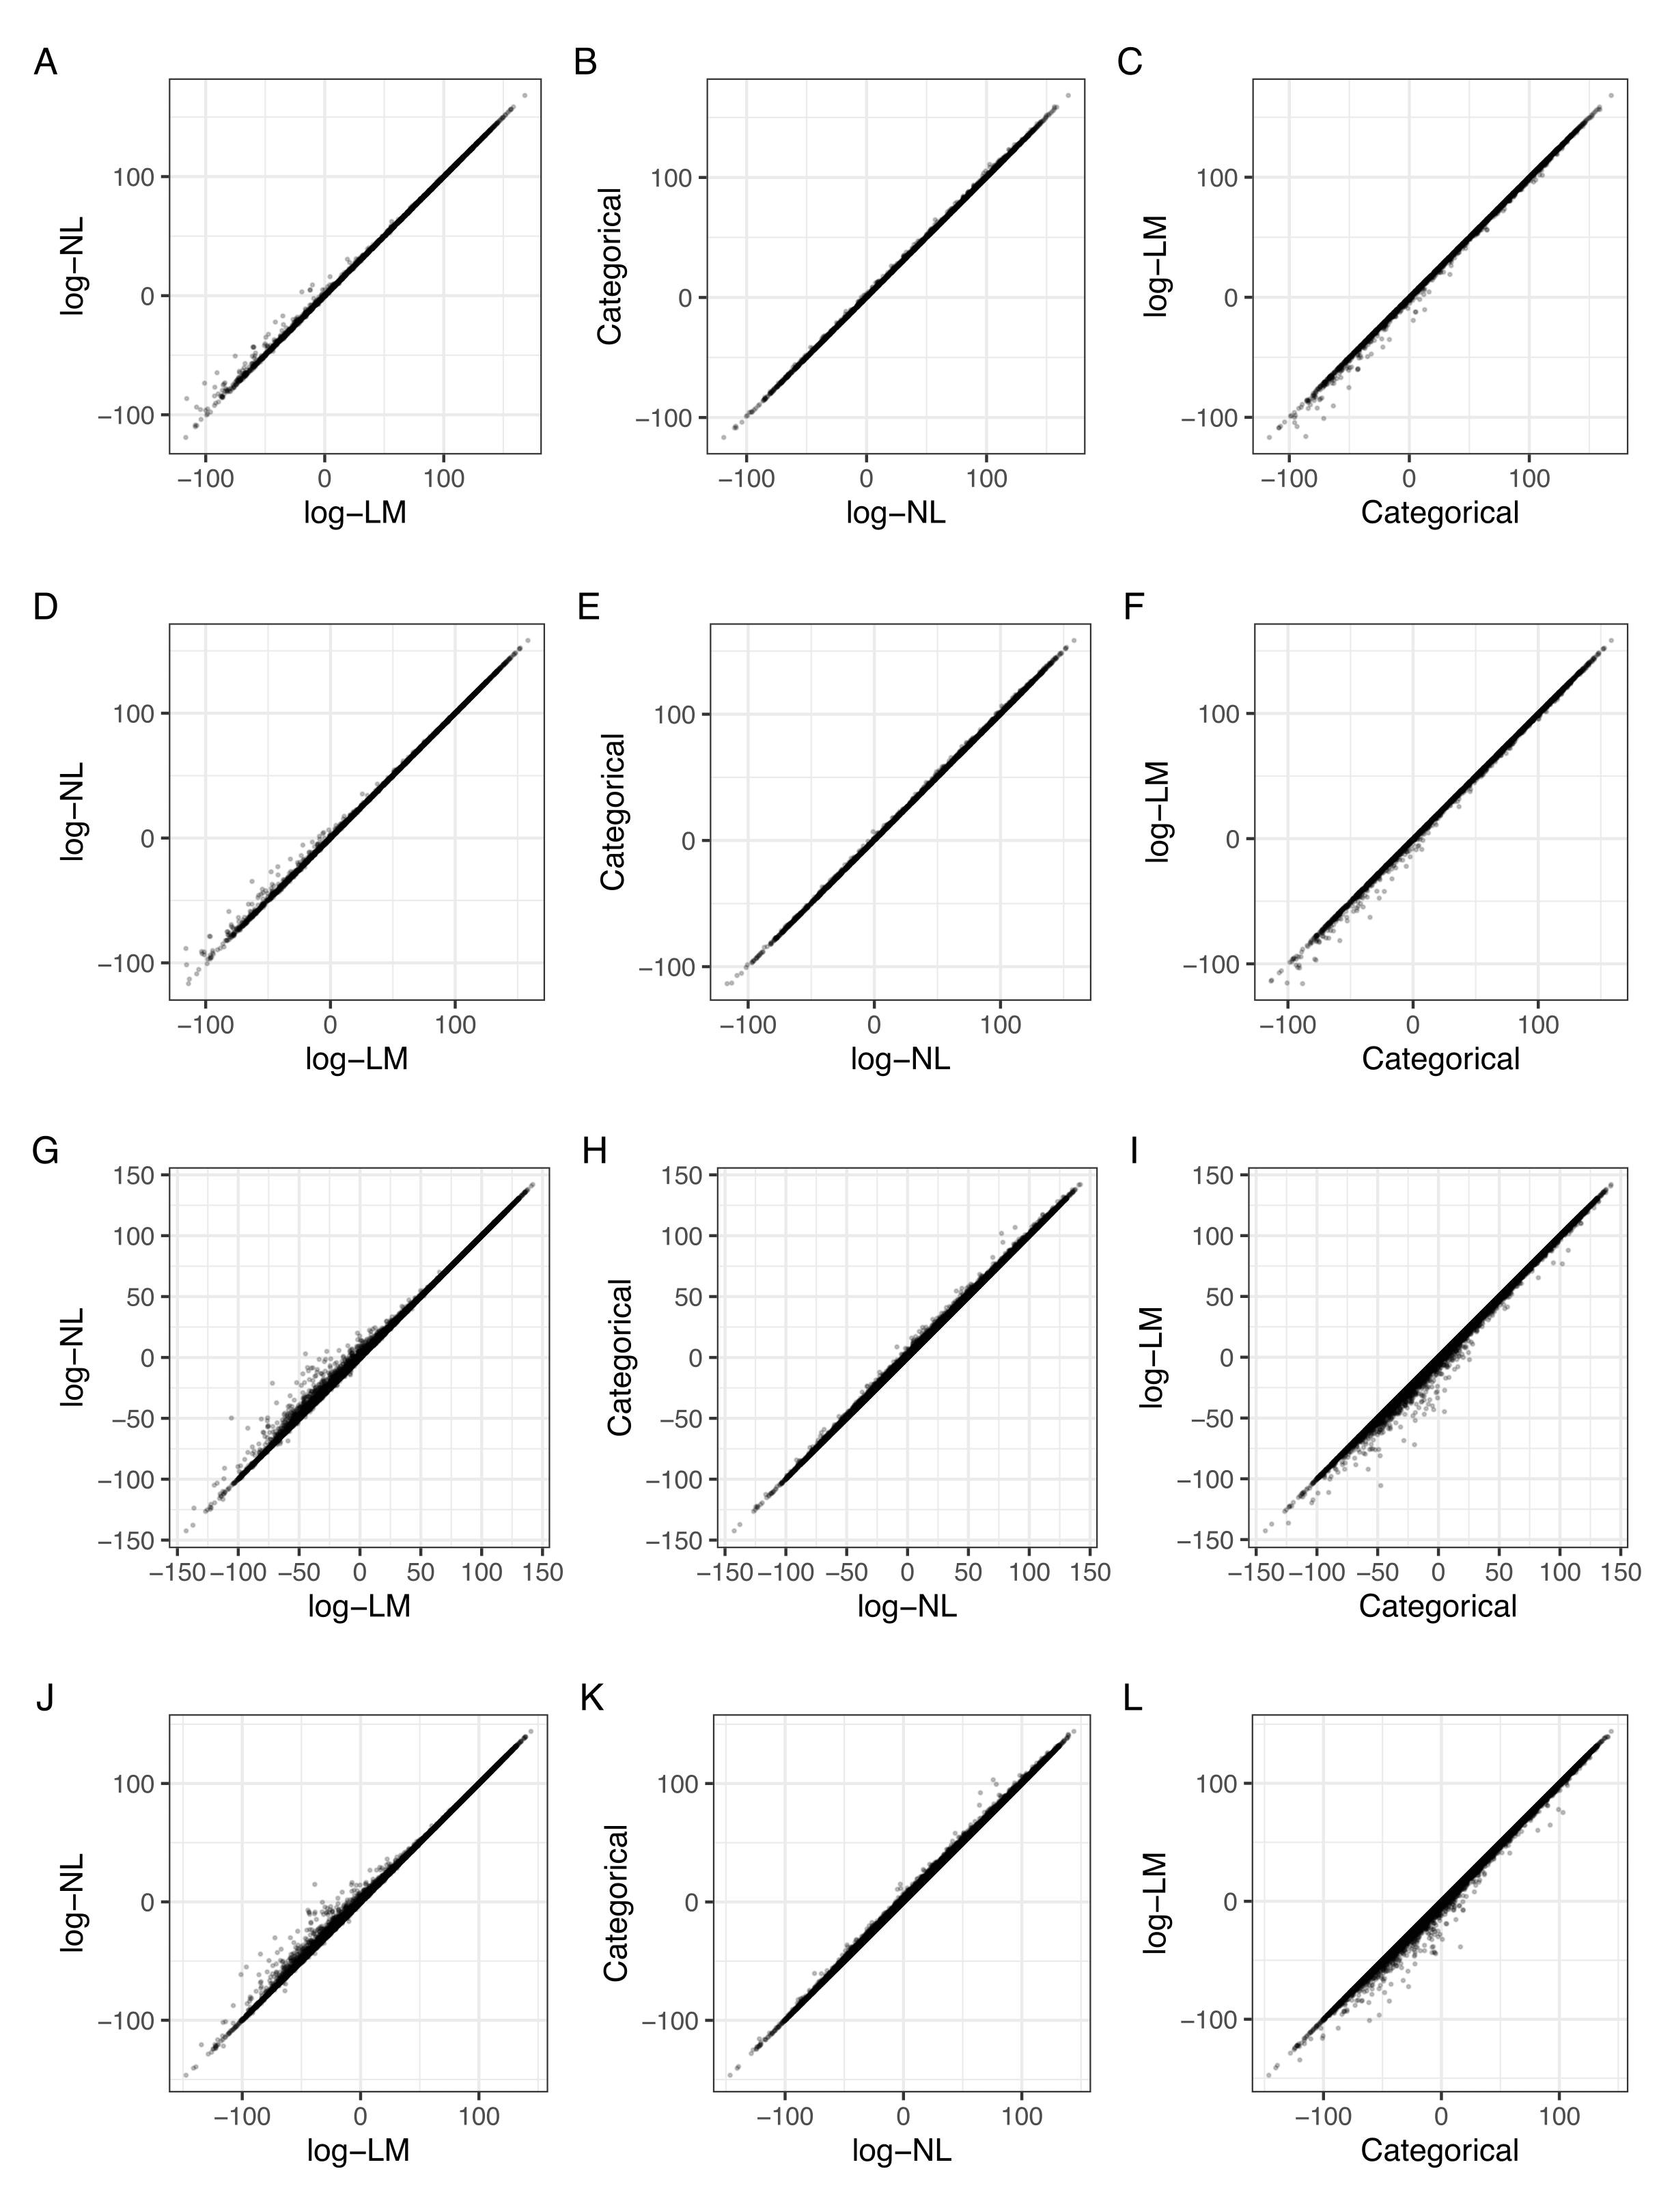
\includegraphics[width=0.7\textwidth]{png/wnt_llk.png}
\end{center}  
\caption{
  {\bf
    S1 Fig.
    Assessing the allelic additivity assumption in hNPCs.}
\textbf{A.} Scatterplots comparing the maximized likelihood between nonlinear and linear regression for 3073 gene-SNP pairs under the control condition. \textbf{B.} The same as in \textbf{A} but between the model with a categorical genotype variable consisting of three levels and nonlinear regression. \textbf{C.} The same as in \textbf{A} but between the model with a categorical genotype variable and linear regression. \textbf{D.} The same as in \textbf{A} but under the treated condition. \textbf{E.} The same as in \textbf{B} but under the treated condition. \textbf{F.} The same as in \textbf{C} but under the treated condition. \textbf{G.} Scatterplots comparing the maximized likelihood between nonlinear and linear regression for 42576 cCRE-SNP pairs under the control condition. \textbf{H.} The same as in \textbf{G} but between the model with a categorical genotype variable and nonlinear regression. \textbf{I.} The same as in \textbf{G} but between the model with a categorical genotype variable and linear regression. \textbf{J.} The same as in \textbf{G} but under the treated condition. \textbf{K.} The same as in \textbf{H} but under the treated condition. \textbf{L.} The same as in \textbf{I} but under the treated condition.
}
\label{s-fig:wnt-llk}
\end{figure}

\begin{figure}[!ht]
\begin{center}
  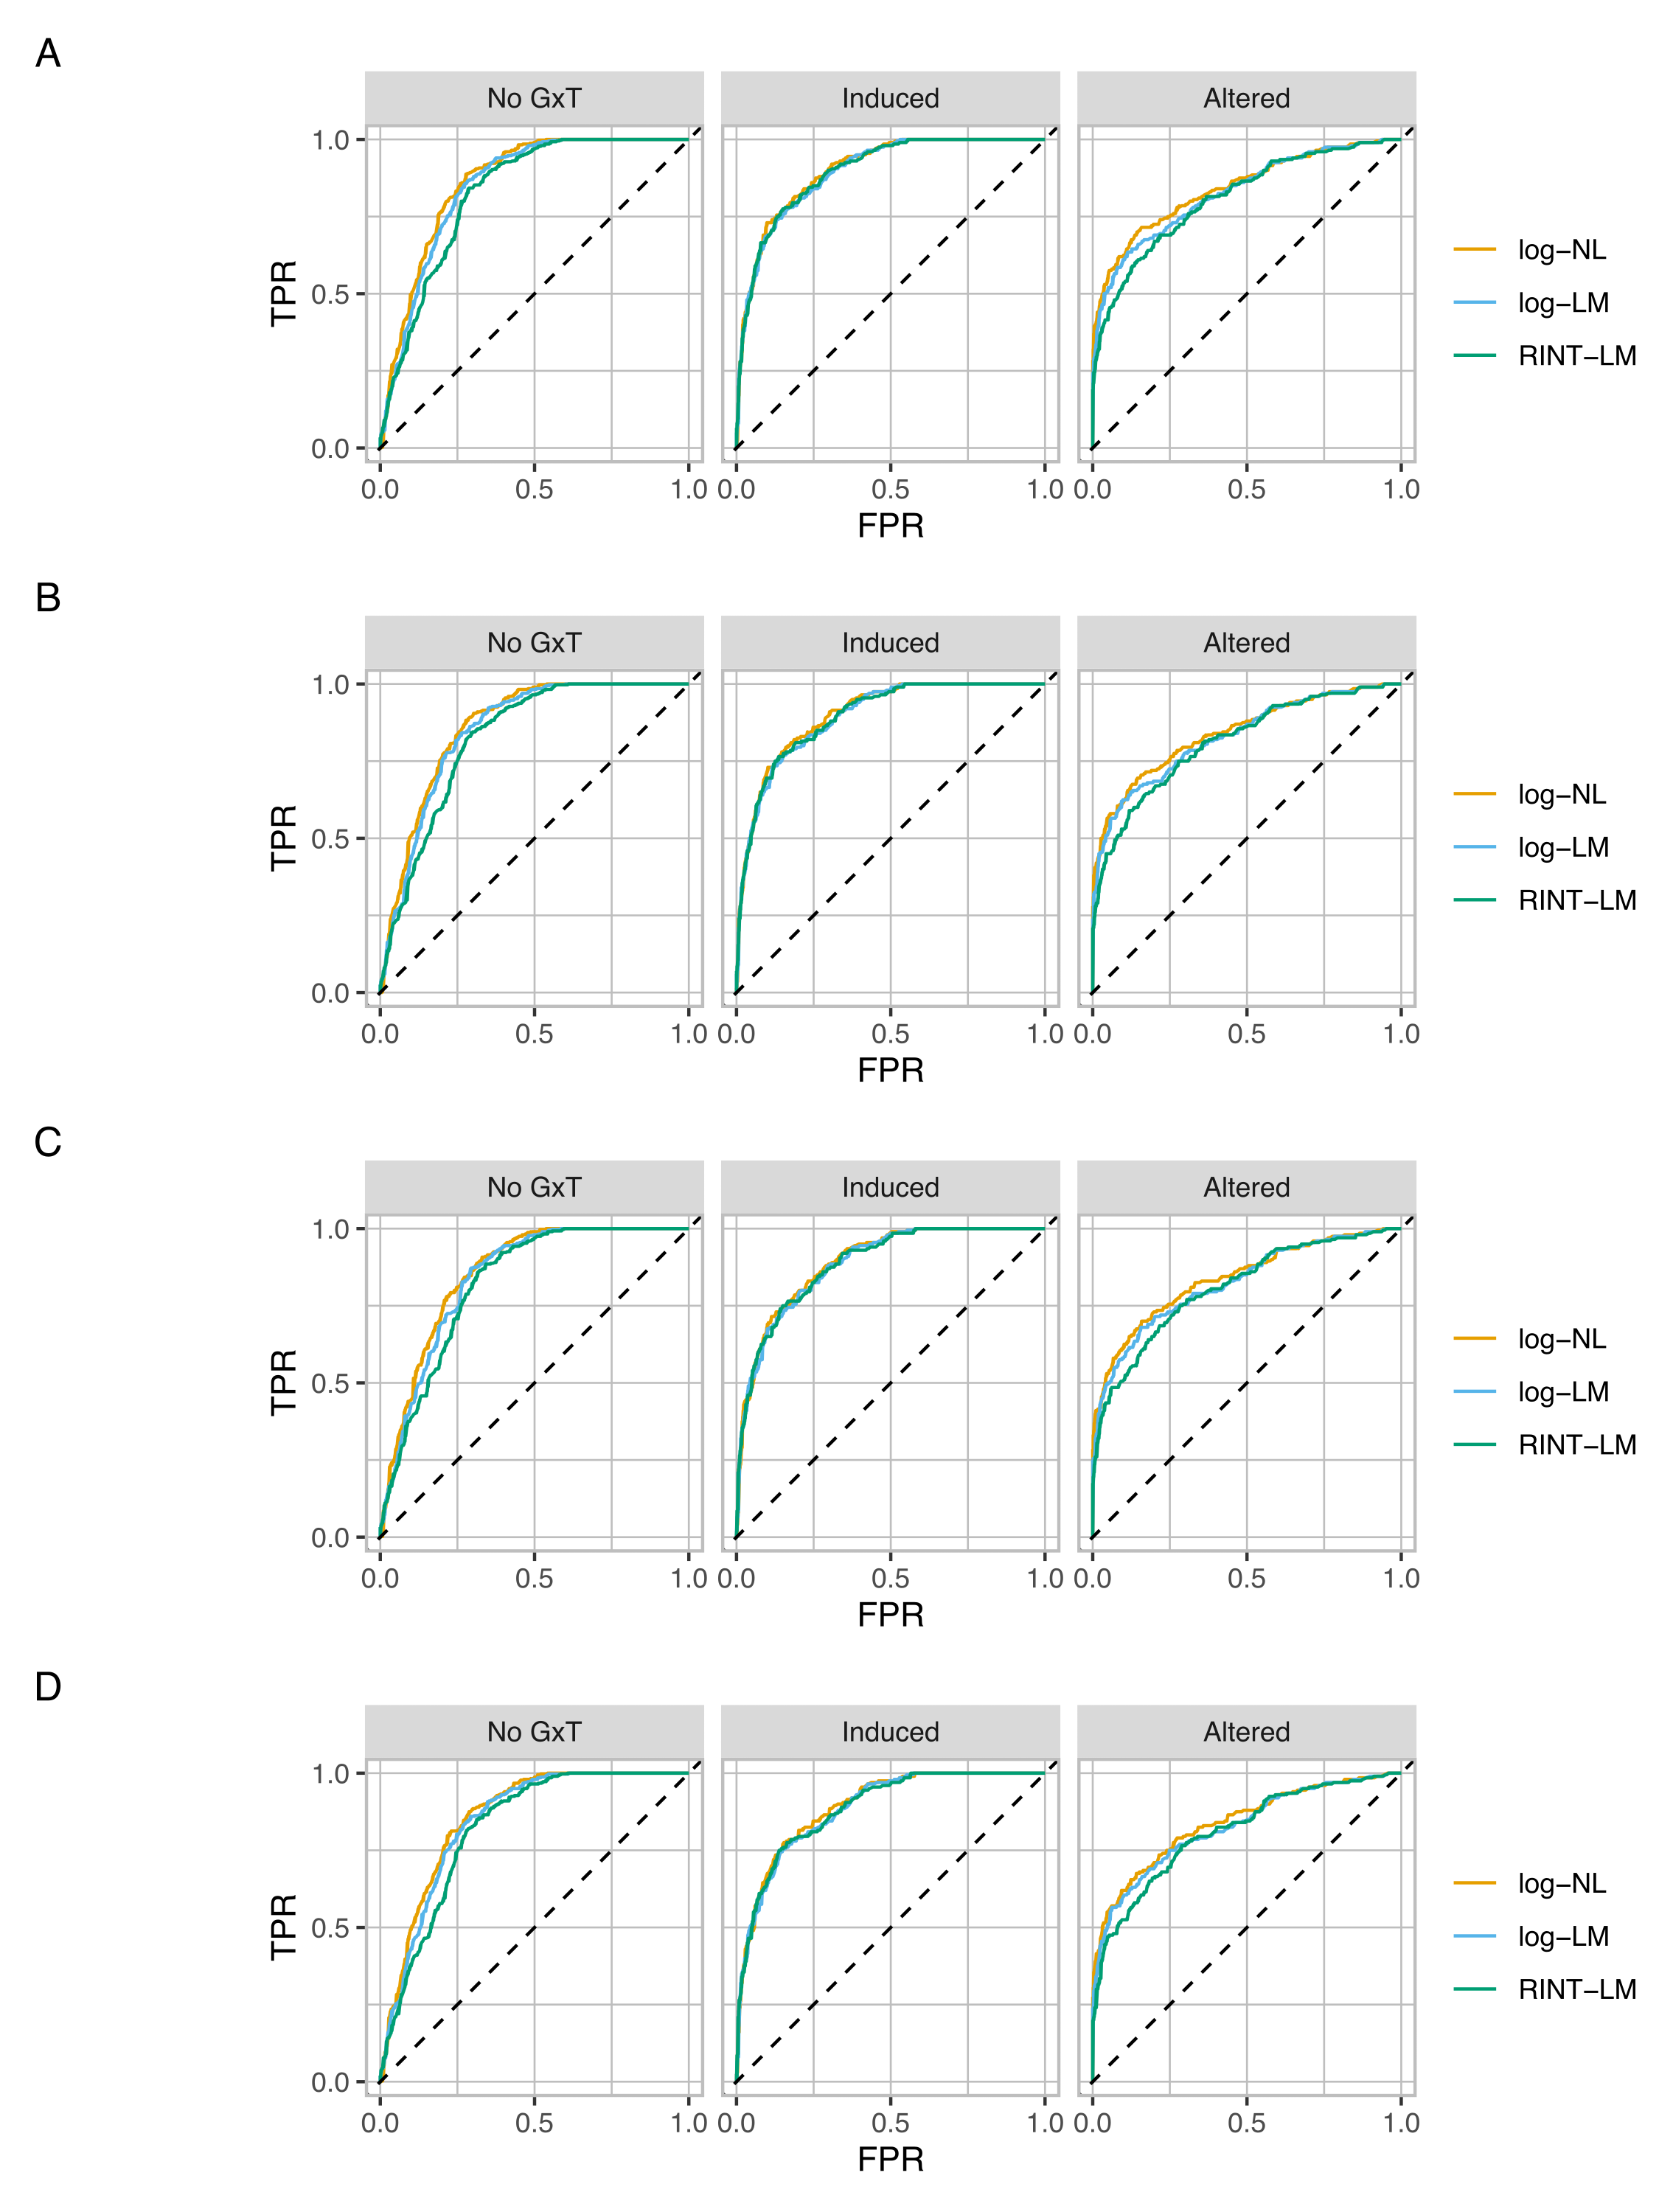
\includegraphics[width=0.8\textwidth]{png/sim_rocc_mcmc_bs.png}
\end{center}
\caption{
  {\bf
    S2 Fig.
    ROC curves assessing the performance of BMS with $\log$-NL, $\log$-LM, and RINT-LM for the no-\GxT, induced, and altered categories using MCMC and bridge sampling.}
Shown are results from 800 simulations without random effect, which we call scenario 1 (\textbf{A}), those with donor random effect in model fitting but not in data generation (scenario 2) (\textbf{B}), those with donor random effect in data generation but not in model fitting (scenario 3) (\textbf{C}), and those with donor effect in both data generation and model fitting (scenario 4) (\textbf{D}).
}
\label{s-fig:sim-rocc-mcmc}
\end{figure}

\begin{figure}[!ht]
\begin{center}
  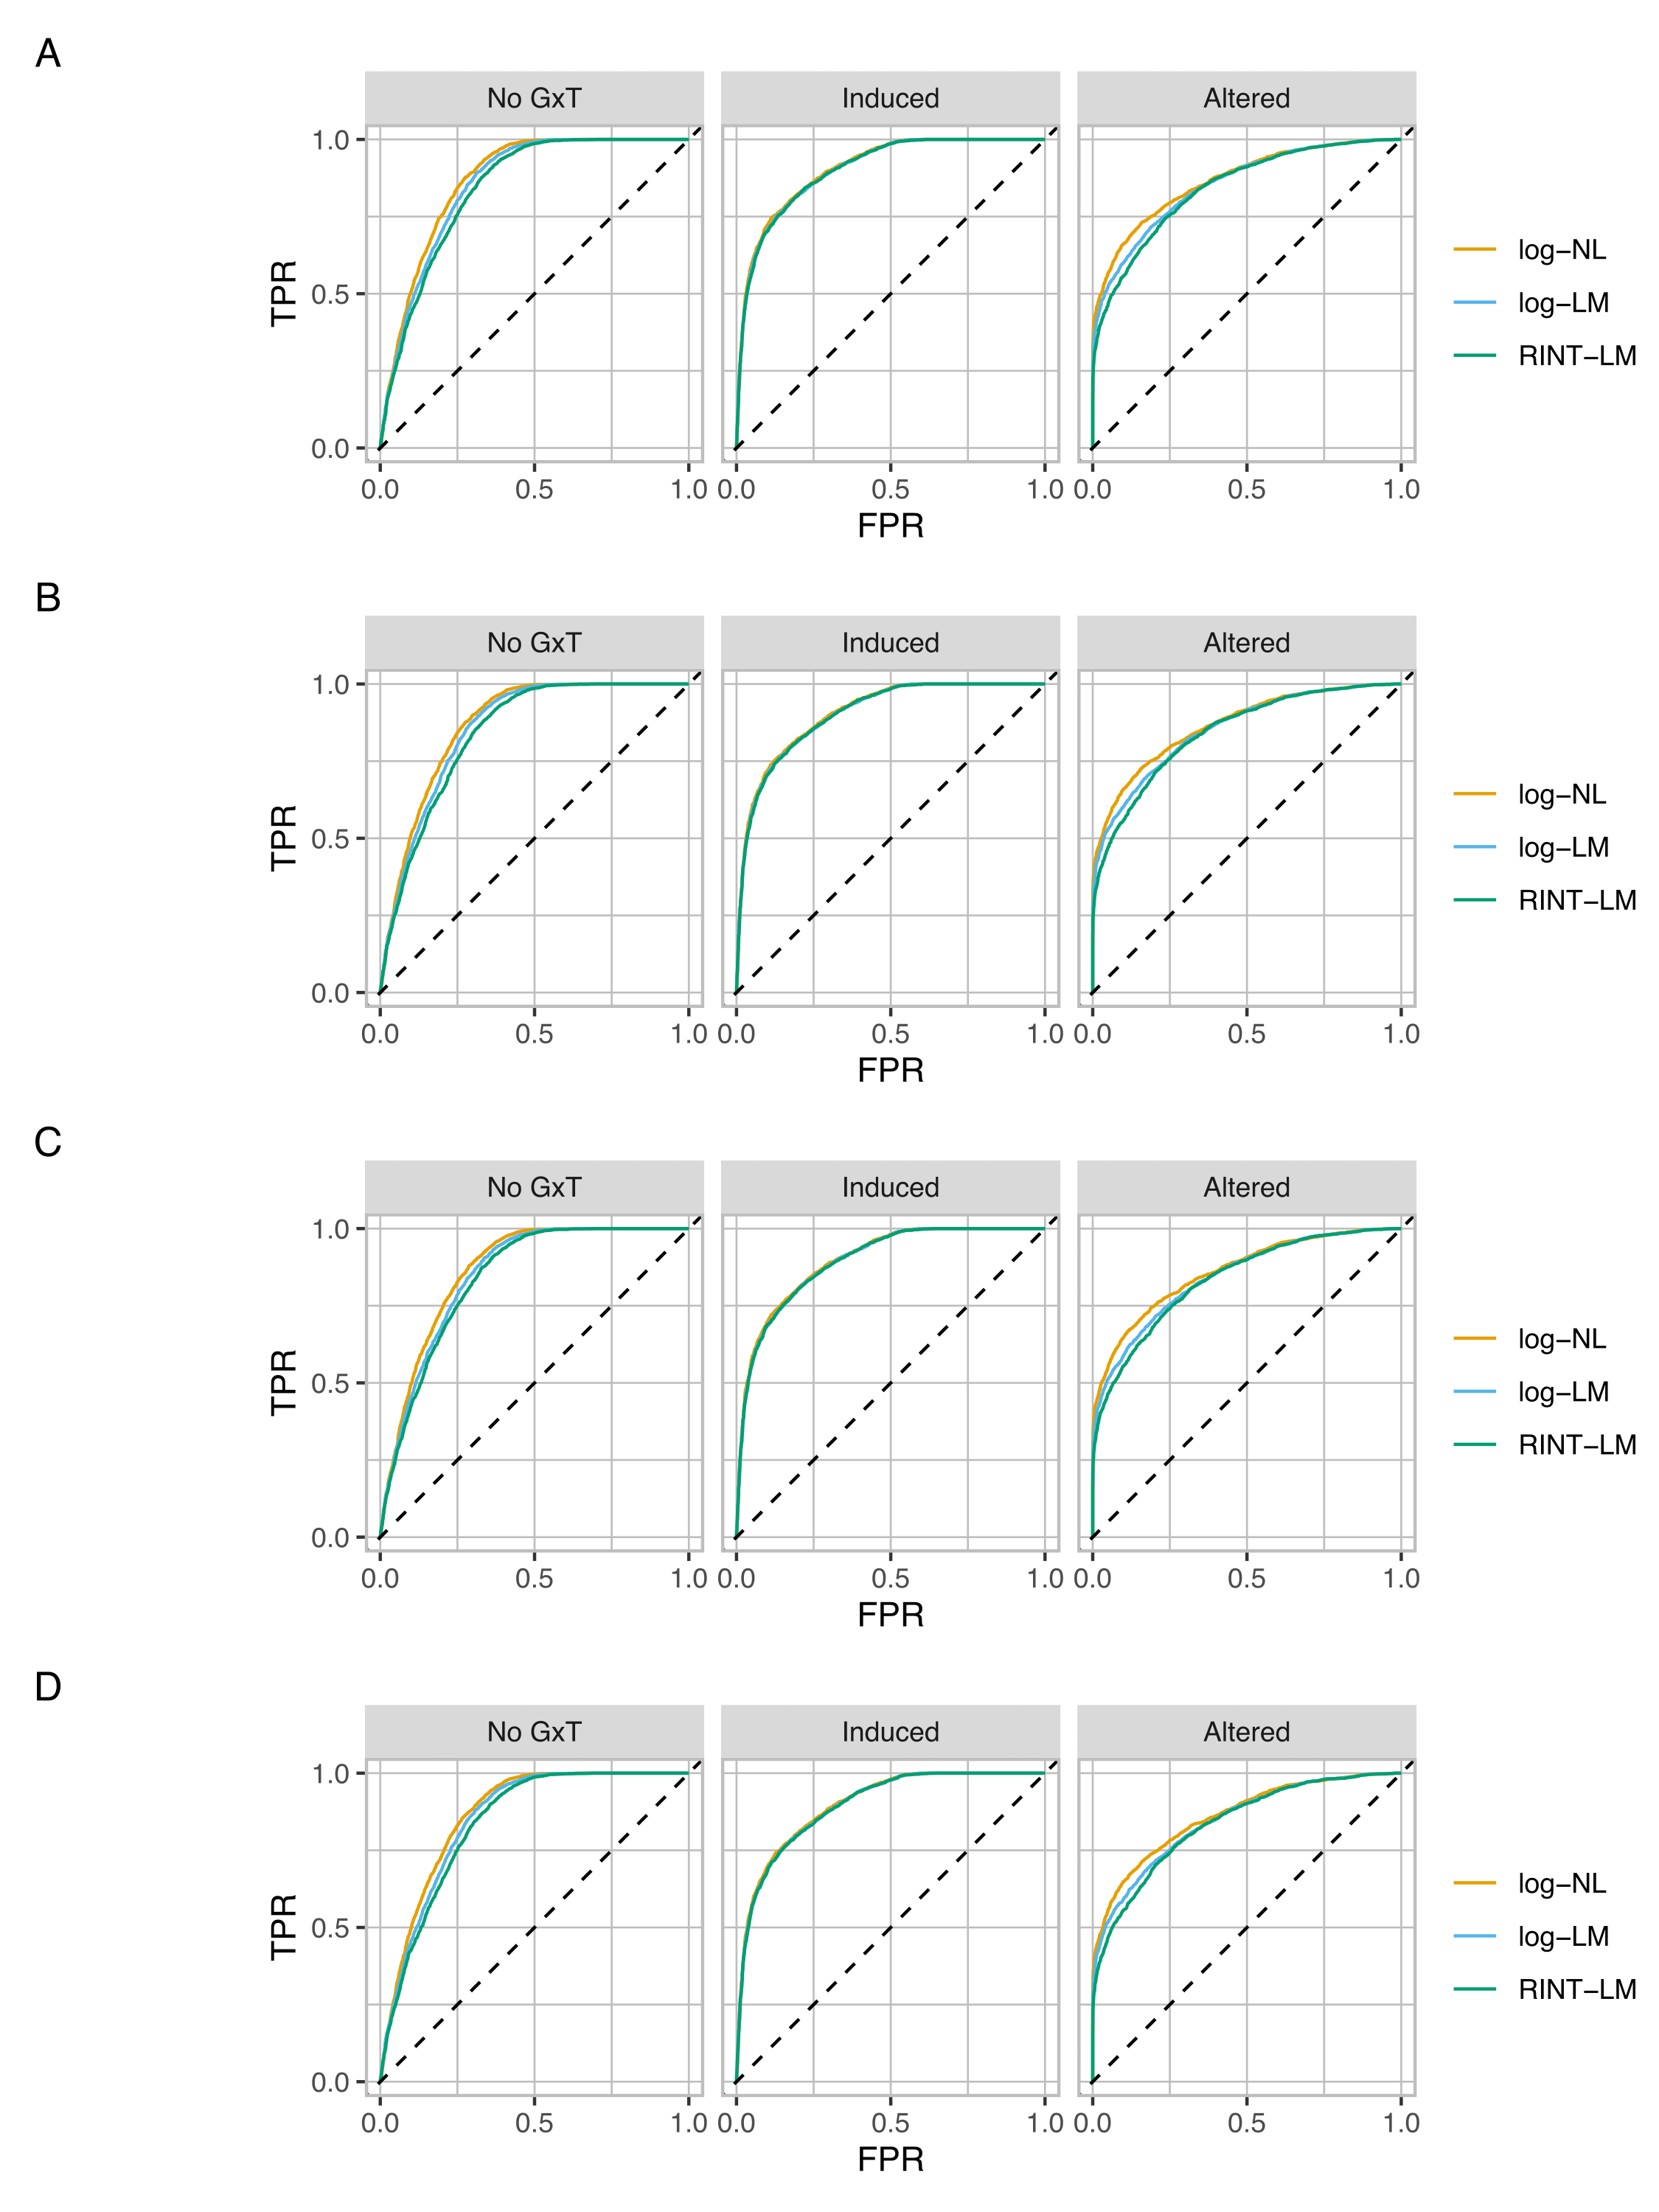
\includegraphics[width=0.8\textwidth]{png/sim_rocc_map_lap.png}
\end{center}  
\caption{
  {\bf
    S2.2 Fig. ROC curves assessing the performance of BMS with $\log$-NL, $\log$-LM, and RINT-LM for the no-\GxT, induced, and altered categories using MAP and Laplace approximation.}
The same as in \sfigroccmcmc but from 8000 simulations using MAP estimation and Laplace approximation.
}
\label{s-fig:sim-rocc-map}
\end{figure}

\begin{figure}[!ht]
\begin{center}
  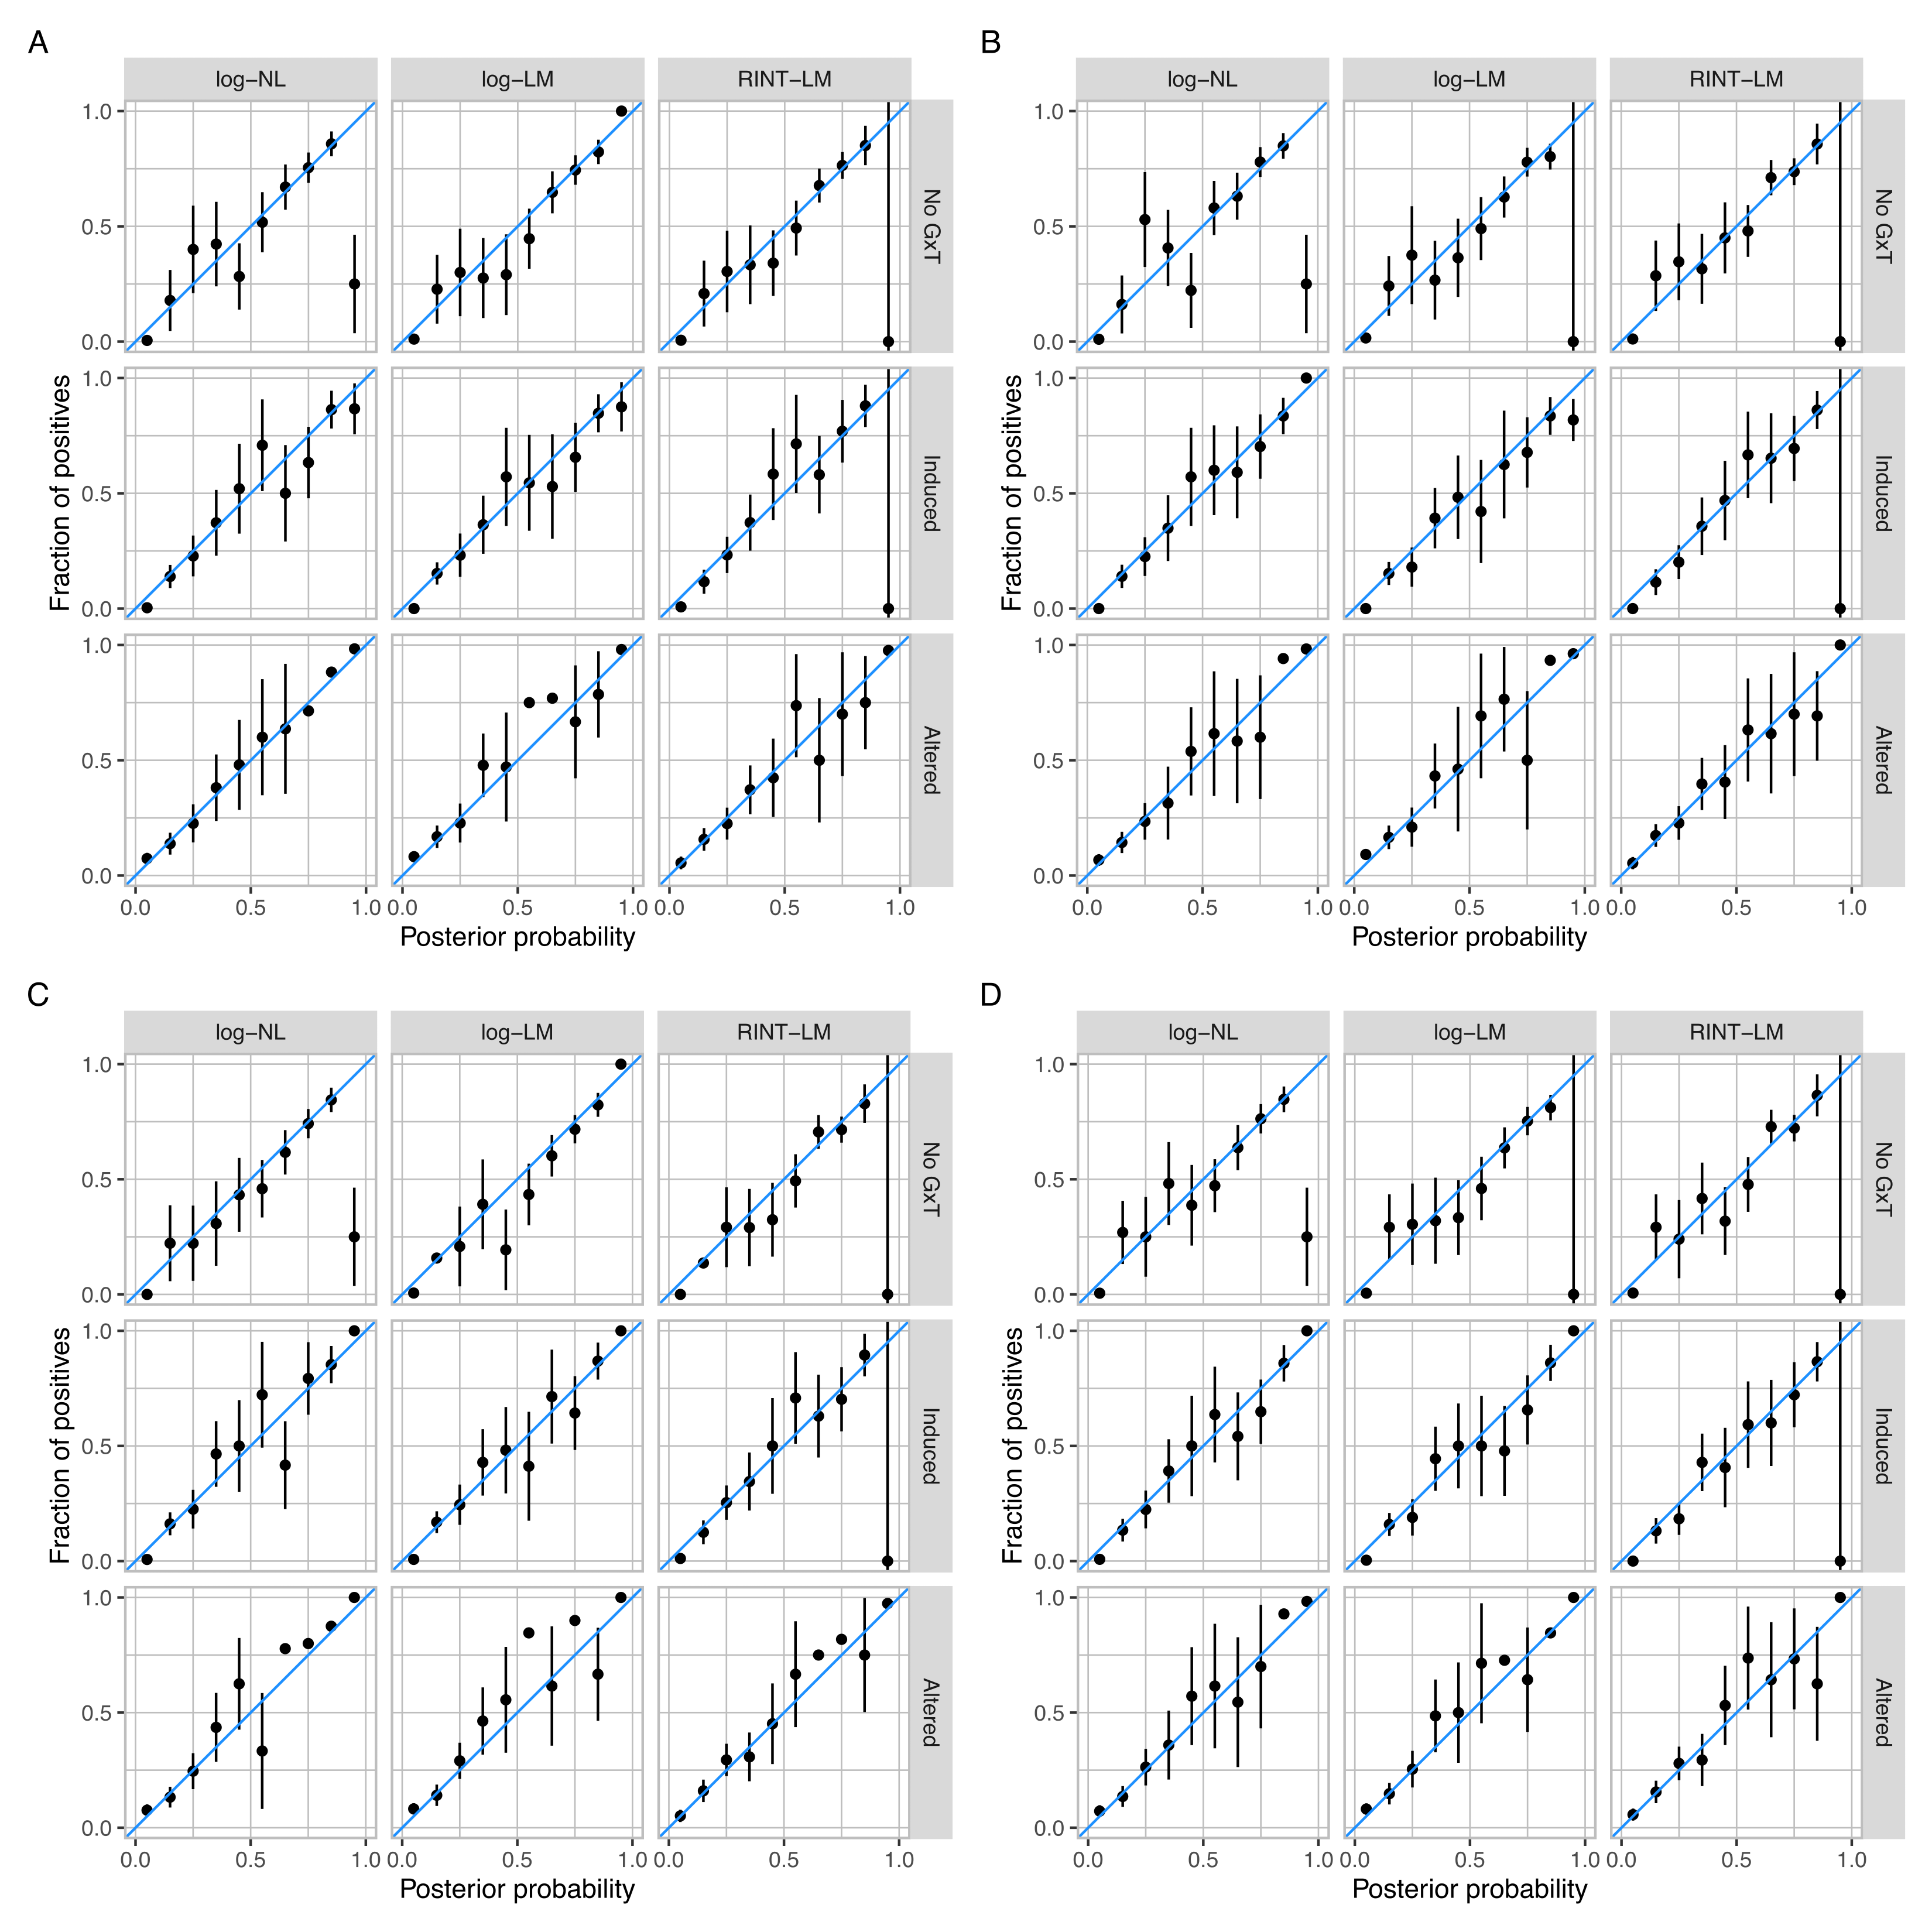
\includegraphics[width=1\textwidth]{png/sim_calib_mcmc_bs.png}
\end{center}  
\caption{
  {\bf
    S3 Fig.
    Calibration of BMS with $\log$-NL, $\log$-LM, and RINT-LM for the no-\GxT, induced, and altered categories using MCMC and bridge sampling.} The $x$- and $y$-axis represent the posterior probability and the fraction of the corresponding events, respectively. The results from 800 simulations are grouped into ten equally-spaced bins. The vertical bars represent the standard errors assuming a binomial distribution. The panels \textbf{A} to \textbf{D} show the results in scenarios 1 to 4, which are described in the legend to \sfigroccmcmc.
}
\label{s-fig:sim-calib-mcmc}
\end{figure}

\begin{figure}[!ht]
\begin{center}
  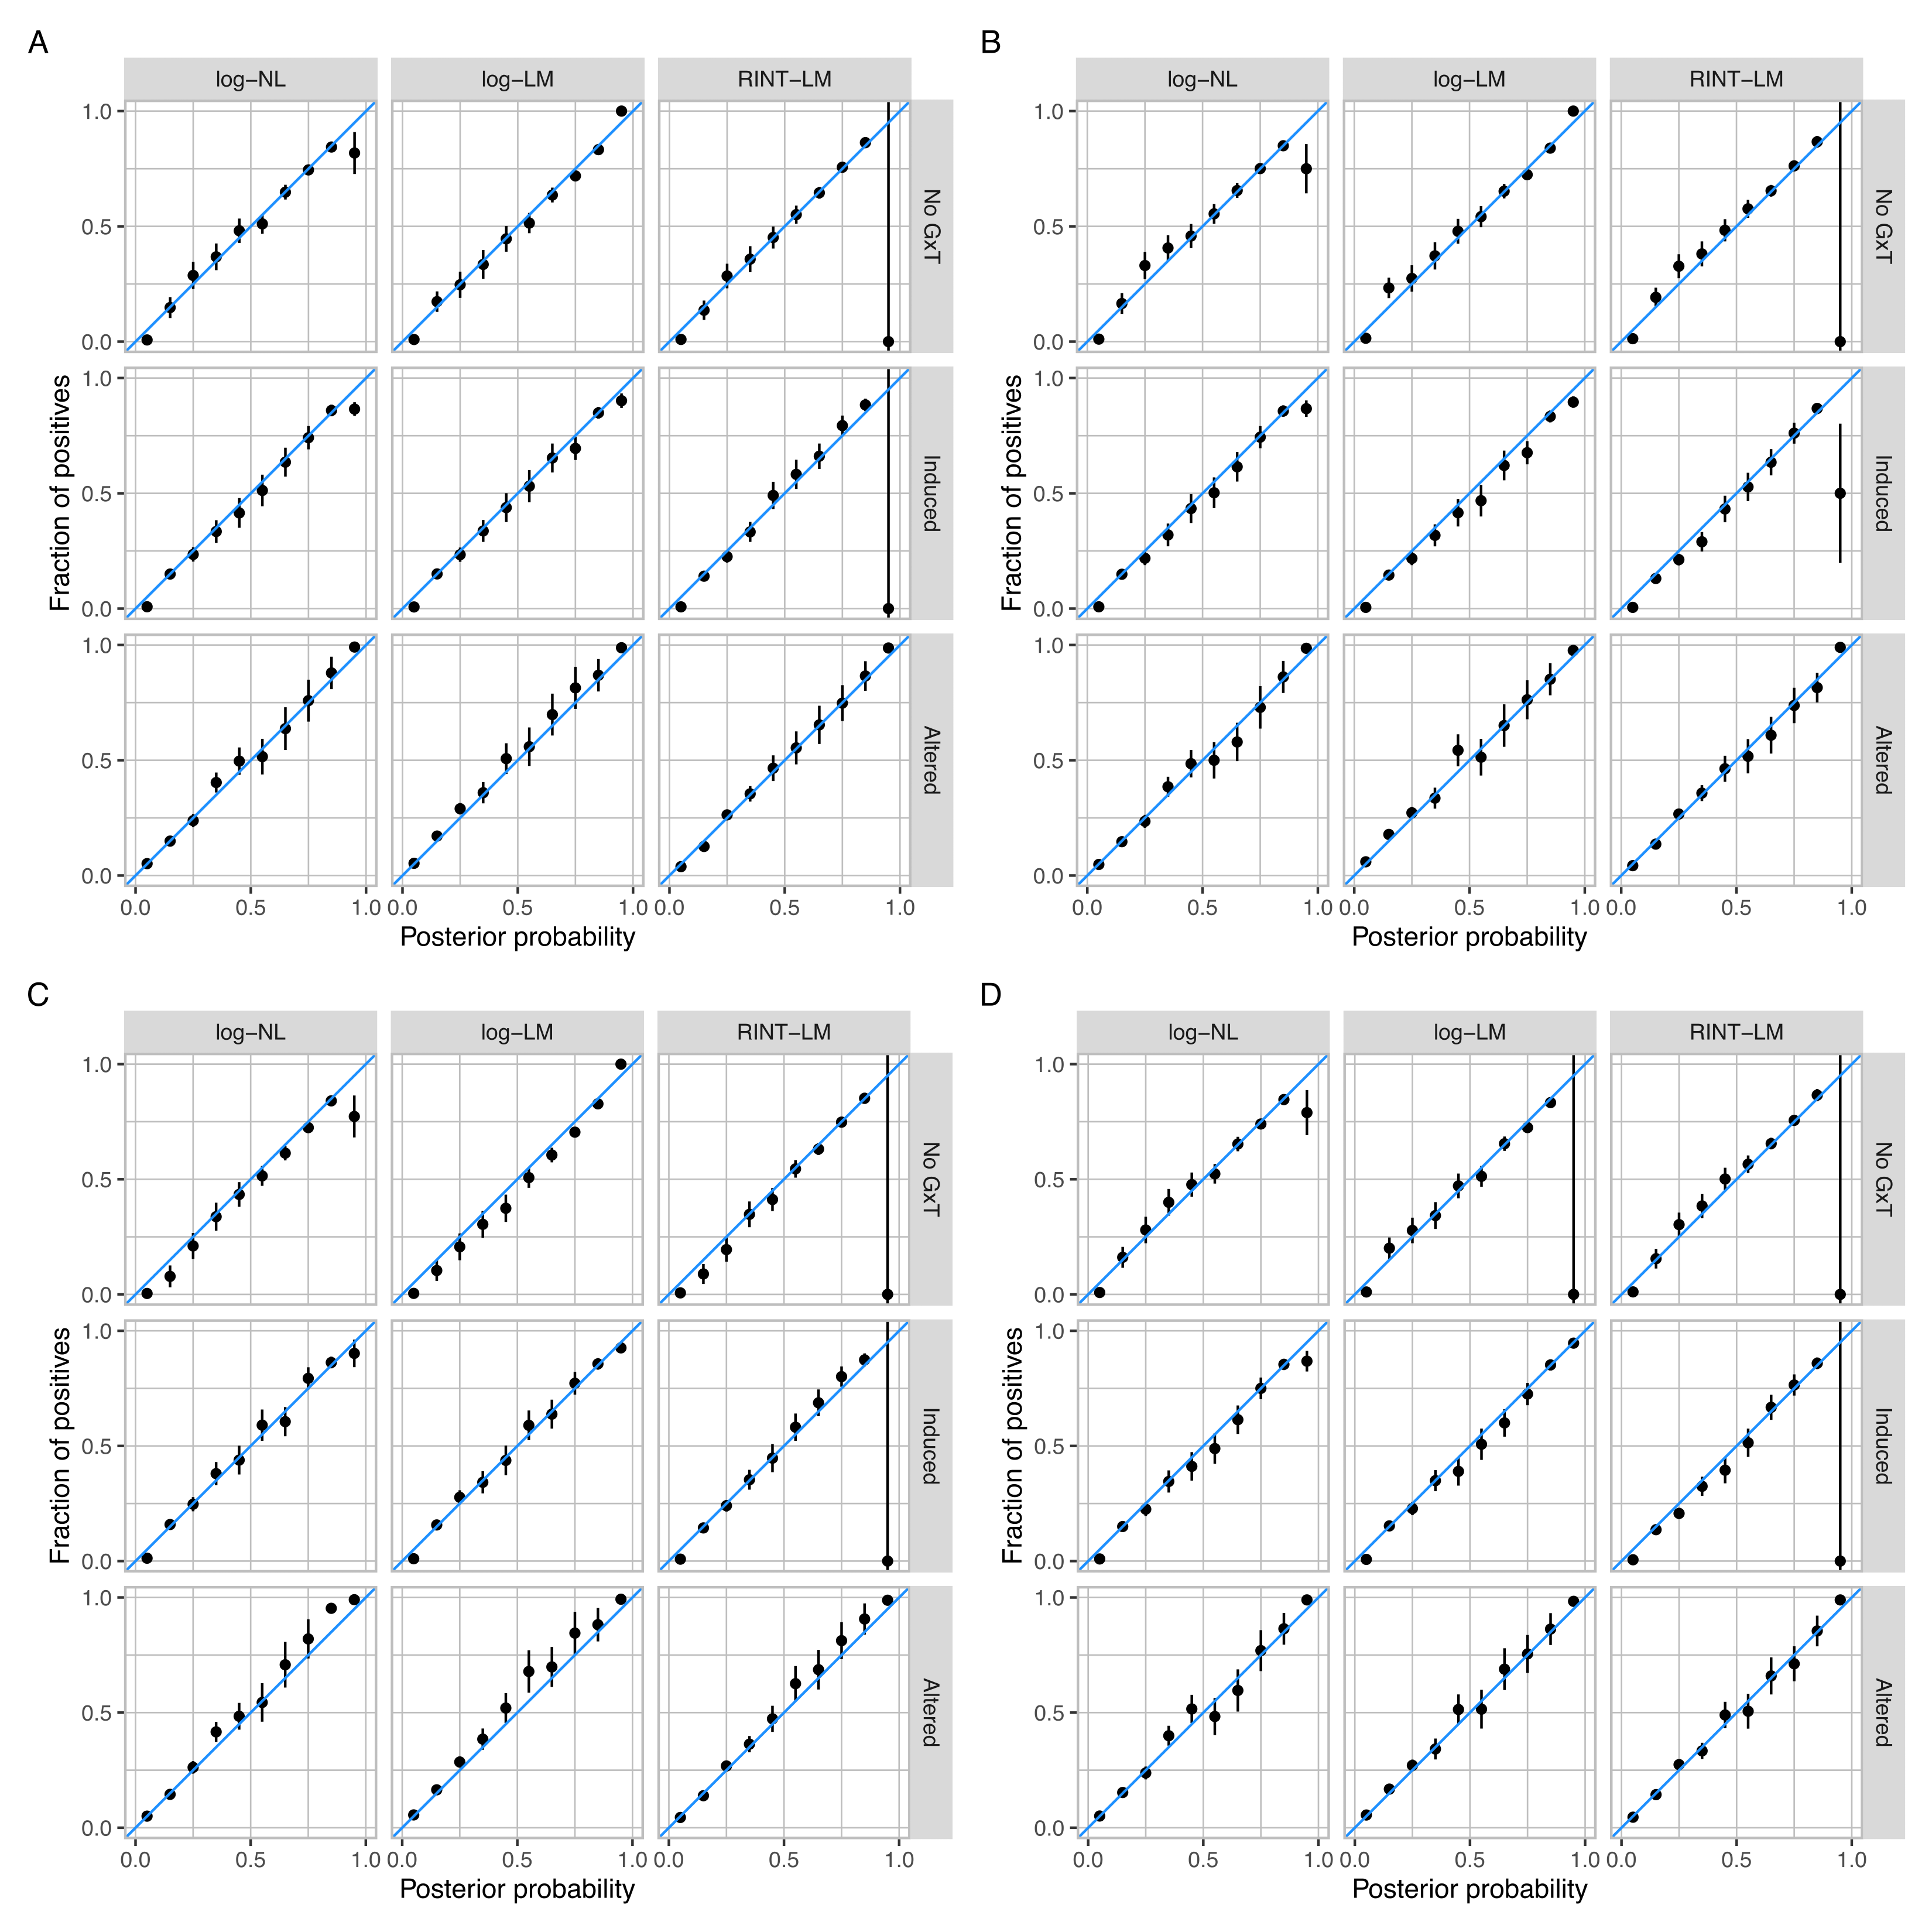
\includegraphics[width=1\textwidth]{png/sim_calib_map_lap.png}
\end{center}  
\caption{
  {\bf
    S3.2 Fig. Calibration of BMS with $\log$-NL, $\log$-LM, and RINT-LM for the no-\GxT, induced, and altered categories using MAP and Laplace approximation.}
The same as in \sfigroccmcmc but from 8000 simulations using MAP estimation and Laplace approximation.
}
\label{s-fig:sim-calib-map}
\end{figure}

\begin{figure}[!ht]
\begin{center}
  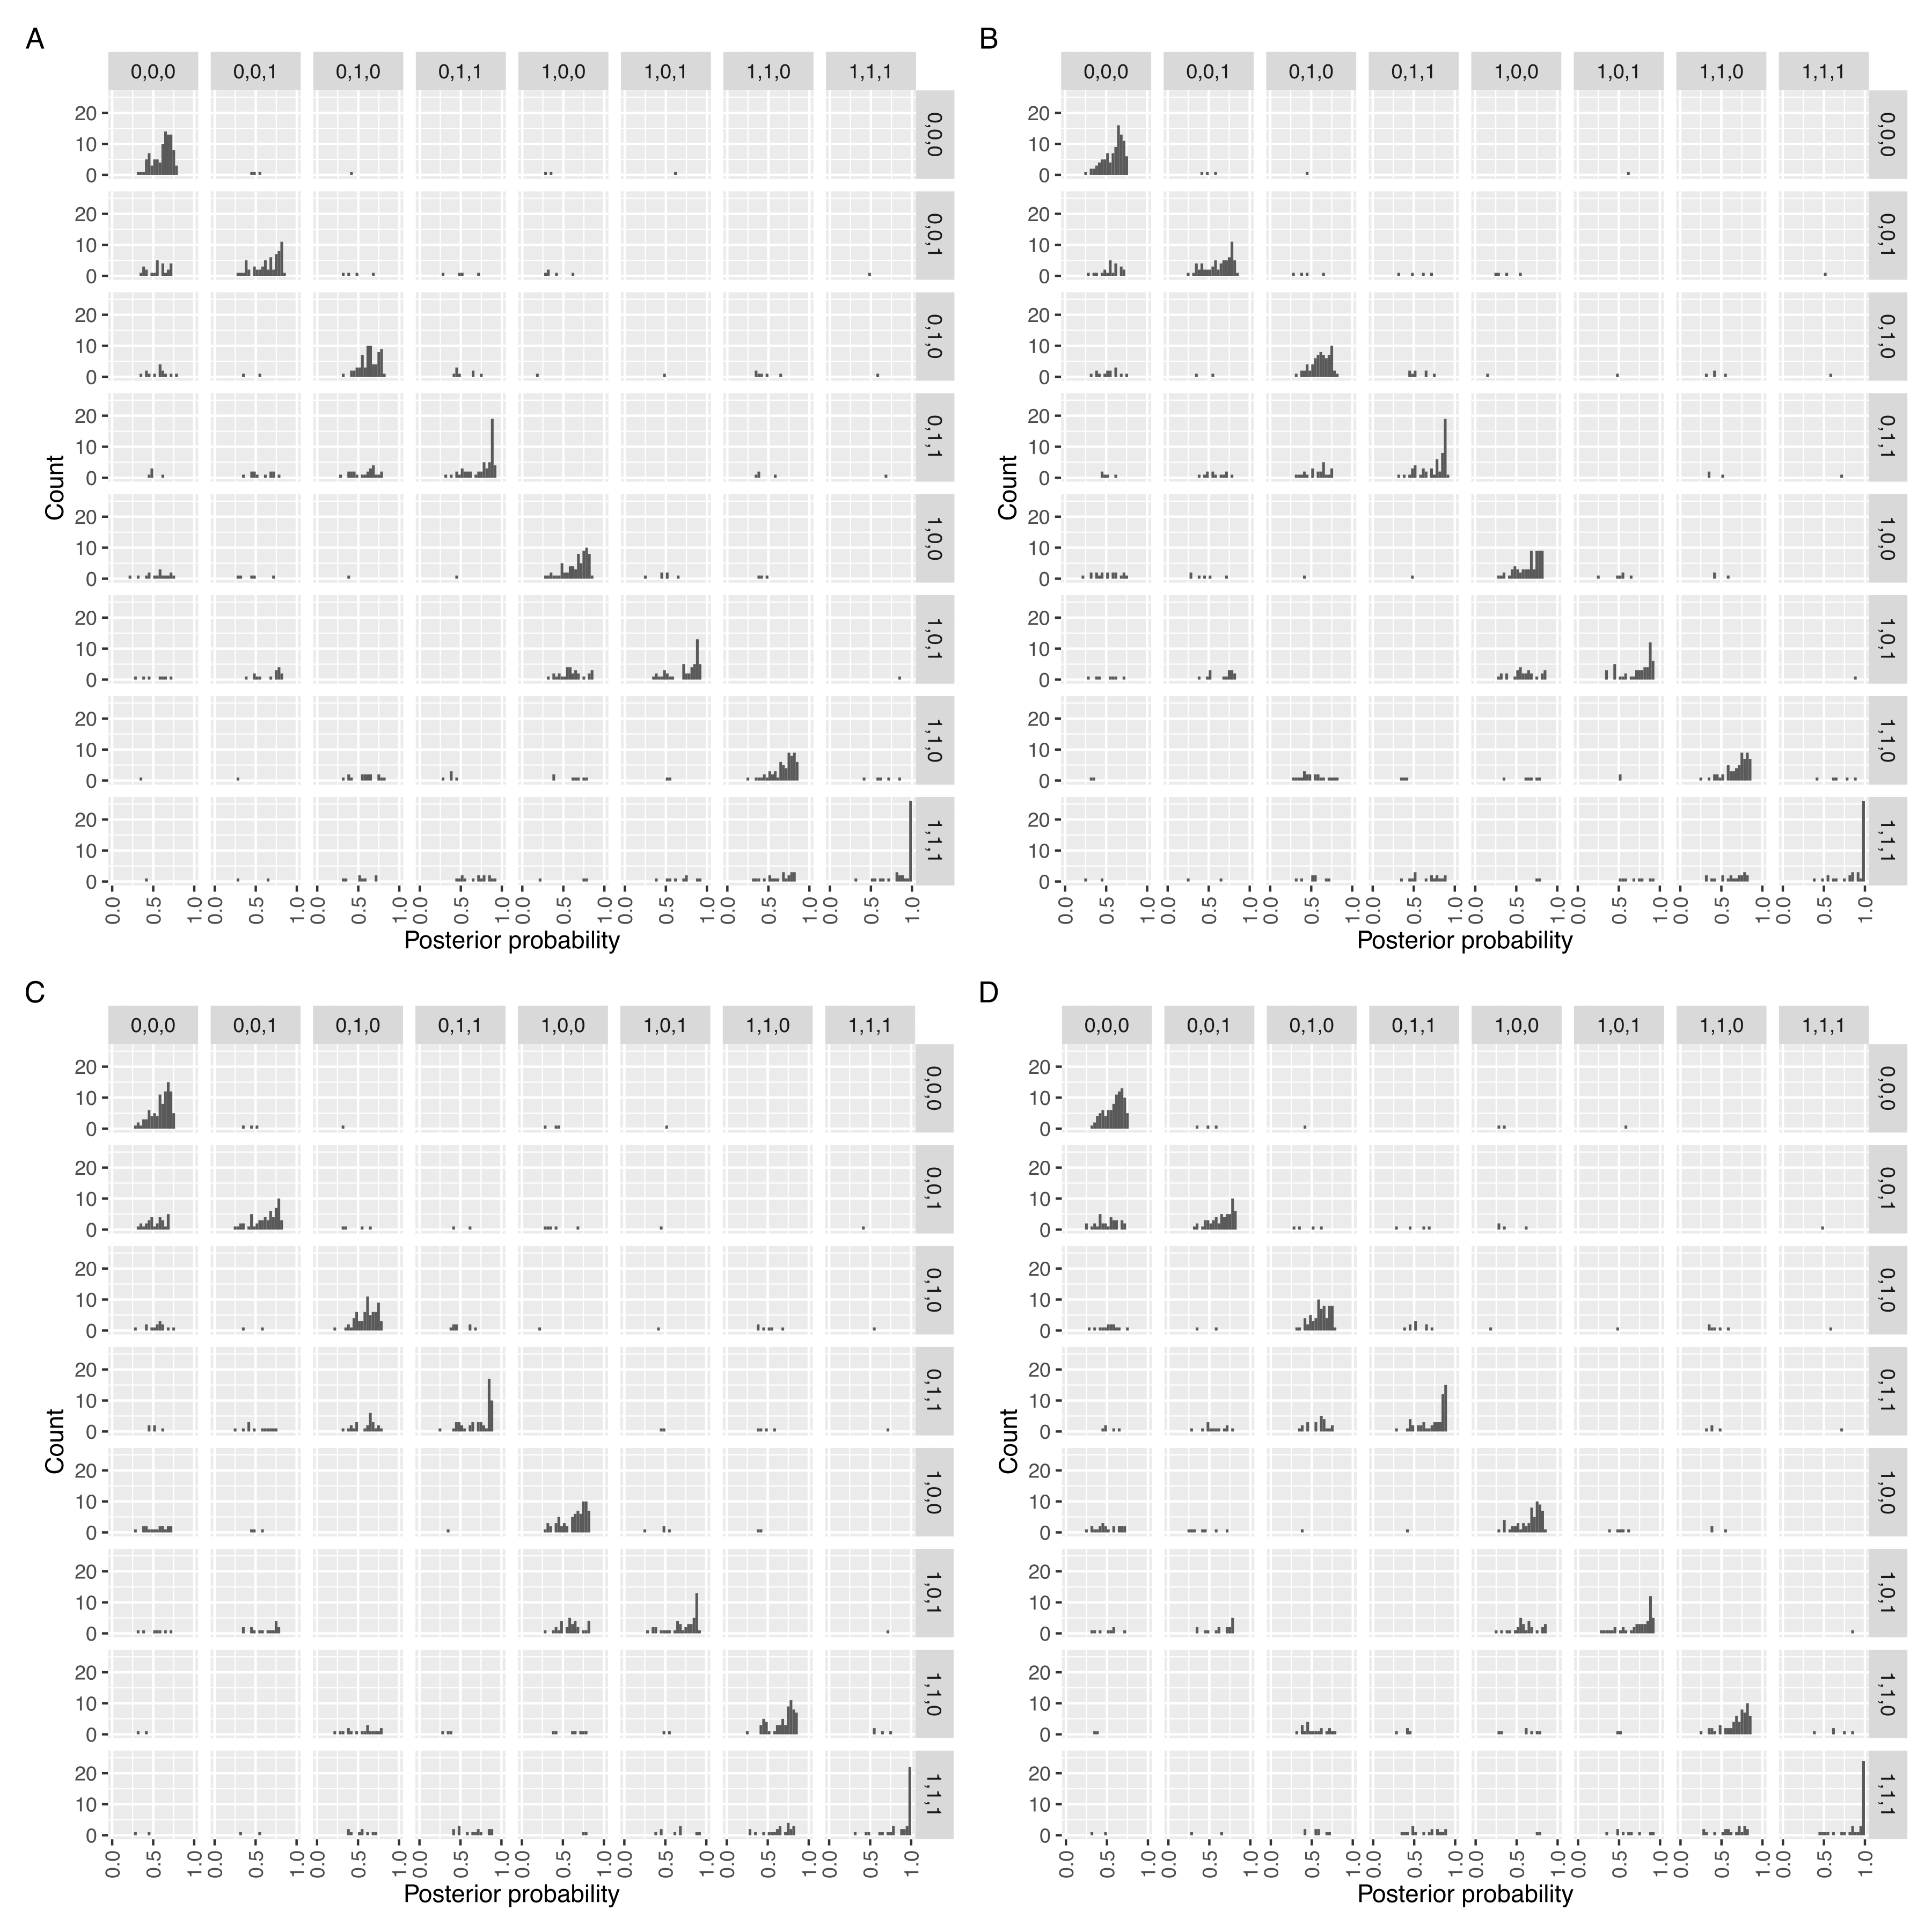
\includegraphics[width=1\textwidth]{png/sim_hist_mcmc_bs_nl.png}
\end{center}  
\caption{
  {\bf
    S4 Fig.
    Stratified histograms of posterior probability of the eight models obtained by BMS with $\log$-NL using MCMC and bridge sampling.}
In each panel, the rows and columns represent the data-generating and posterior mode models, respectively. The panels \textbf{A} to \textbf{D} show the results in scenarios 1 to 4, which are described in the legend to \sfigroccmcmc.
}
\label{s-fig:sim-hist-mcmc-nl}
\end{figure}

\begin{figure}[!ht]
\begin{center}
  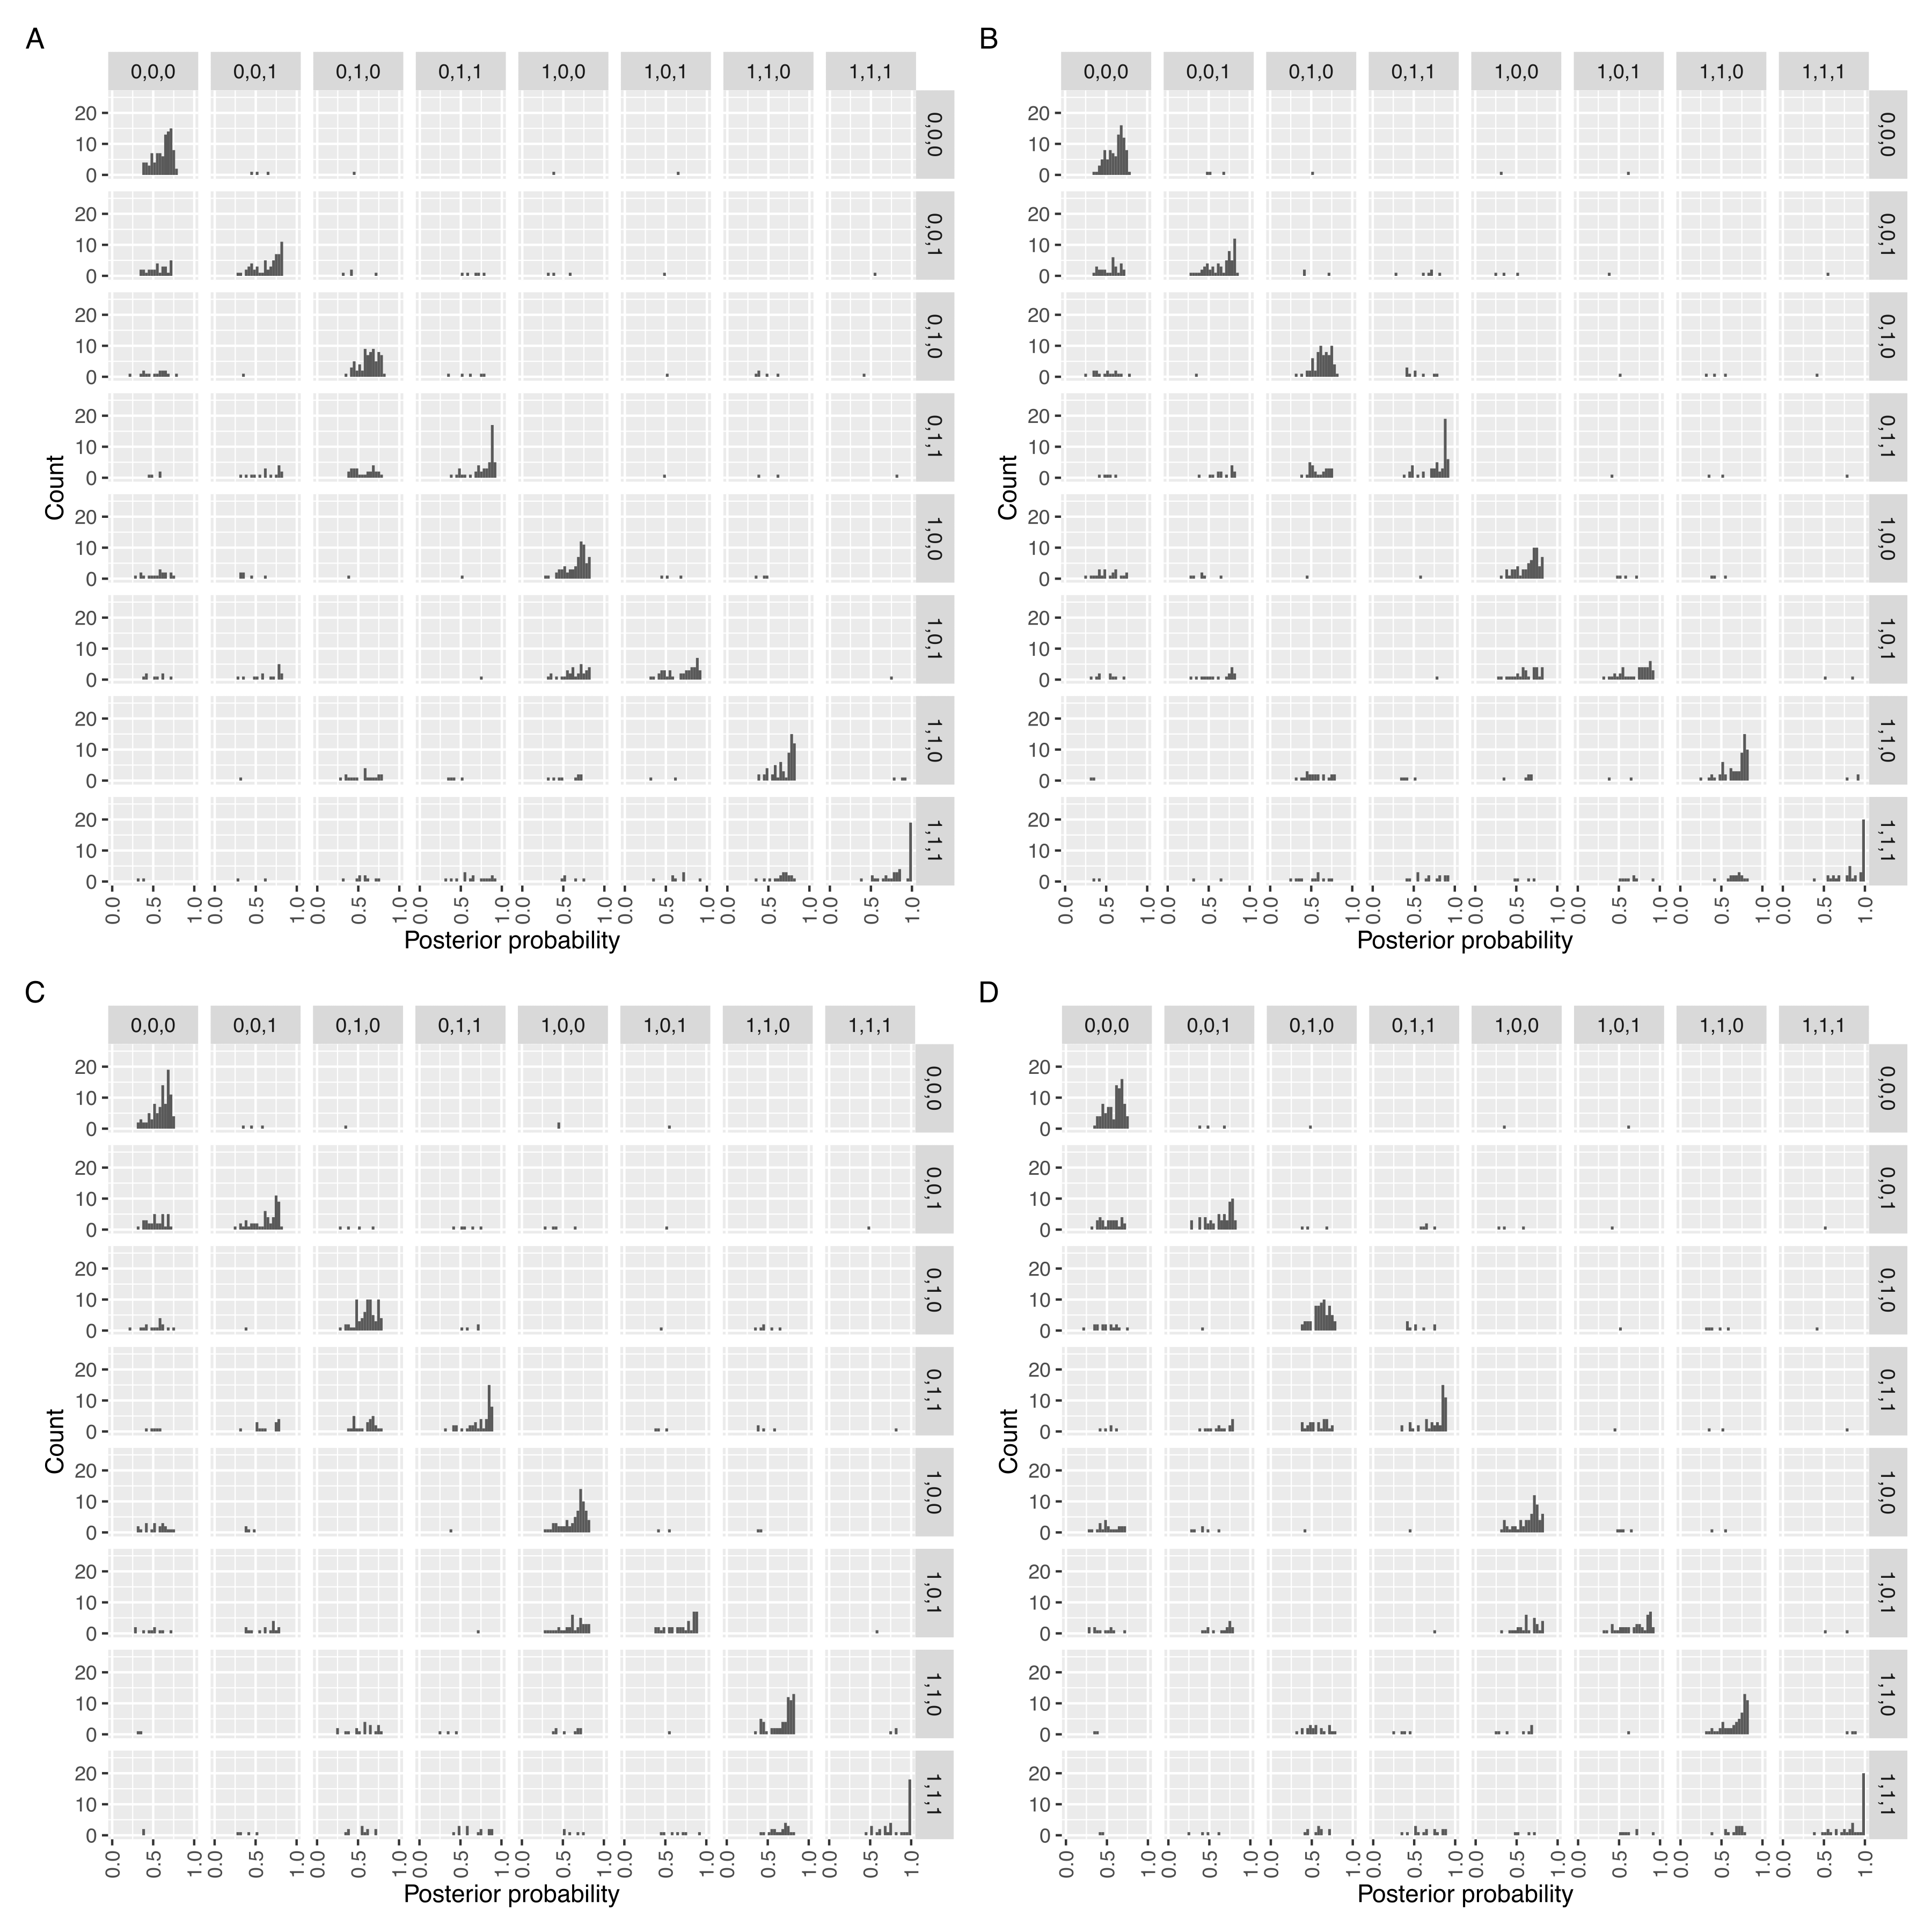
\includegraphics[width=1\textwidth]{png/sim_hist_mcmc_bs_lm.png}
\end{center}  
\caption{
  {\bf
    S4.2 Fig.
    Stratified histograms of posterior probability of the eight models obtained by BMS with $\log$-LM using MCMC and bridge sampling.}
The same as in \sfighistmcmcnl but for $\log$-LM.
}
\label{s-fig:sim-hist-mcmc-lm}
\end{figure}

\begin{figure}[!ht]
\begin{center}
  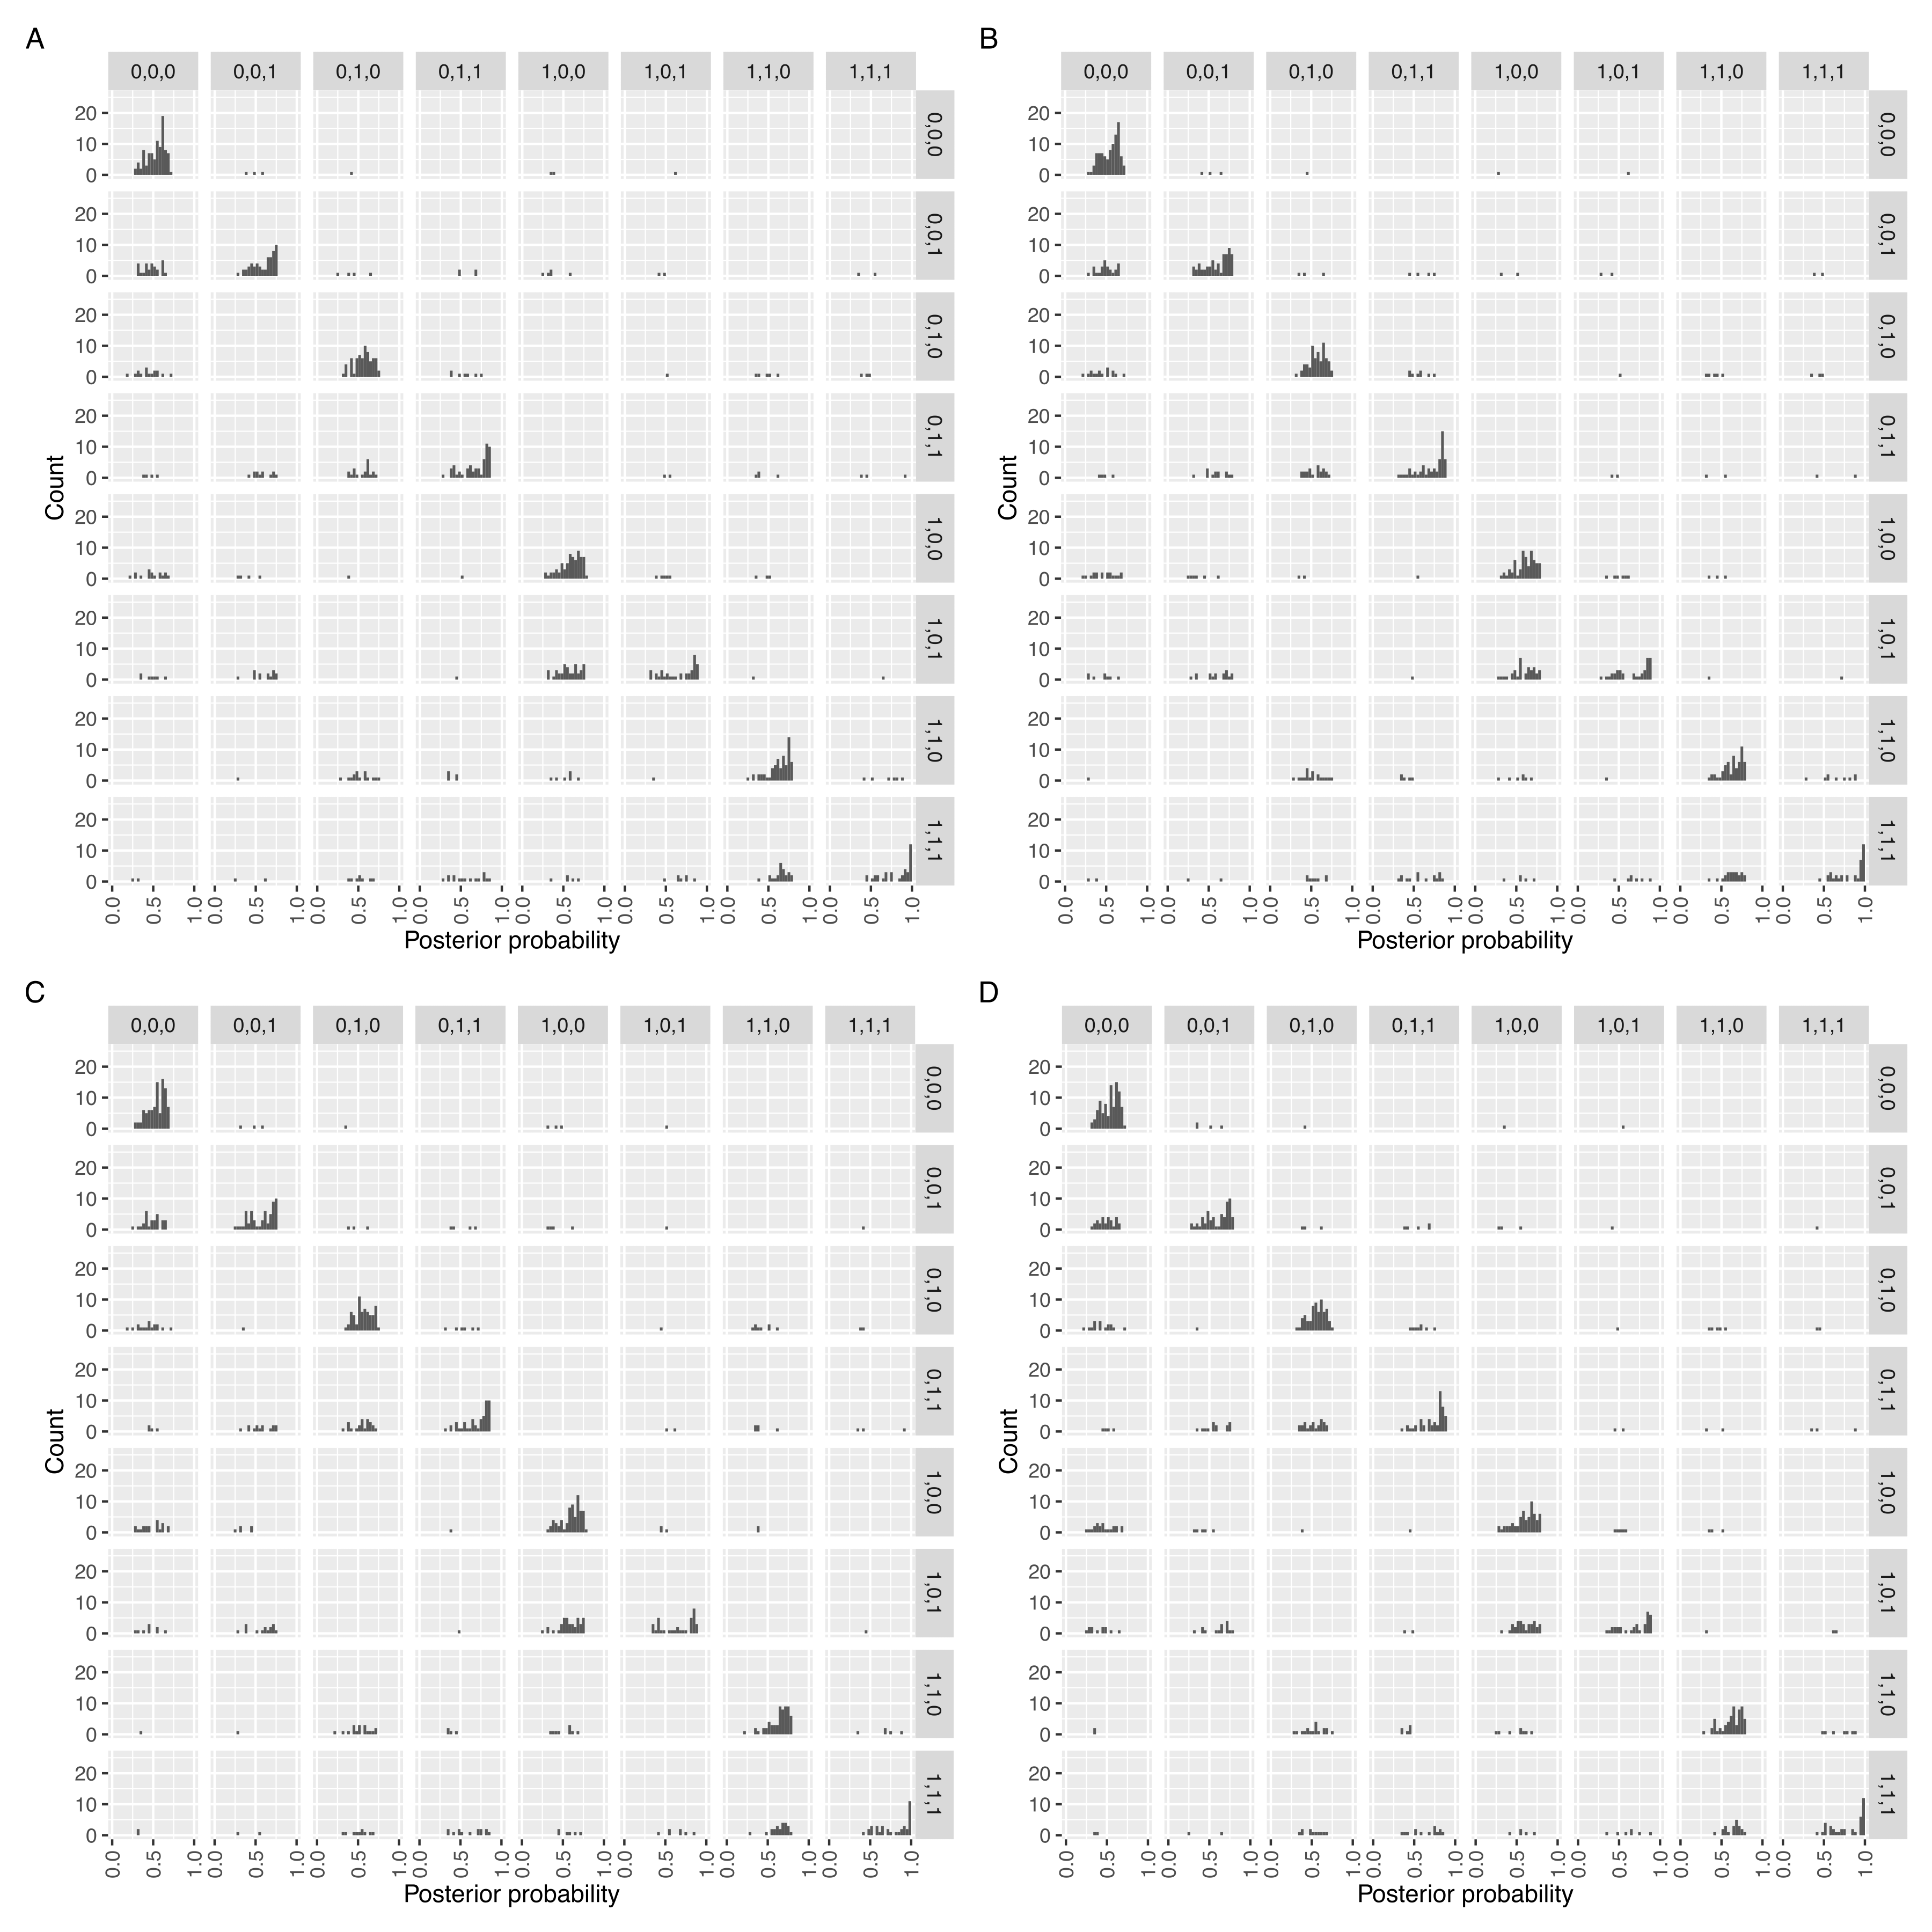
\includegraphics[width=1\textwidth]{png/sim_hist_mcmc_bs_rint.png}
\end{center}  
\caption{
  {\bf
    S4.3 Fig.
    Stratified histograms of posterior probability of the eight models obtained by BMS with RINT-LM using MCMC and bridge sampling.}
The same as in \sfighistmcmcnl but for RINT-LM.
}
\label{s-fig:sim-hist-mcmc-rint}
\end{figure}

\begin{figure}[!ht]
\begin{center}
  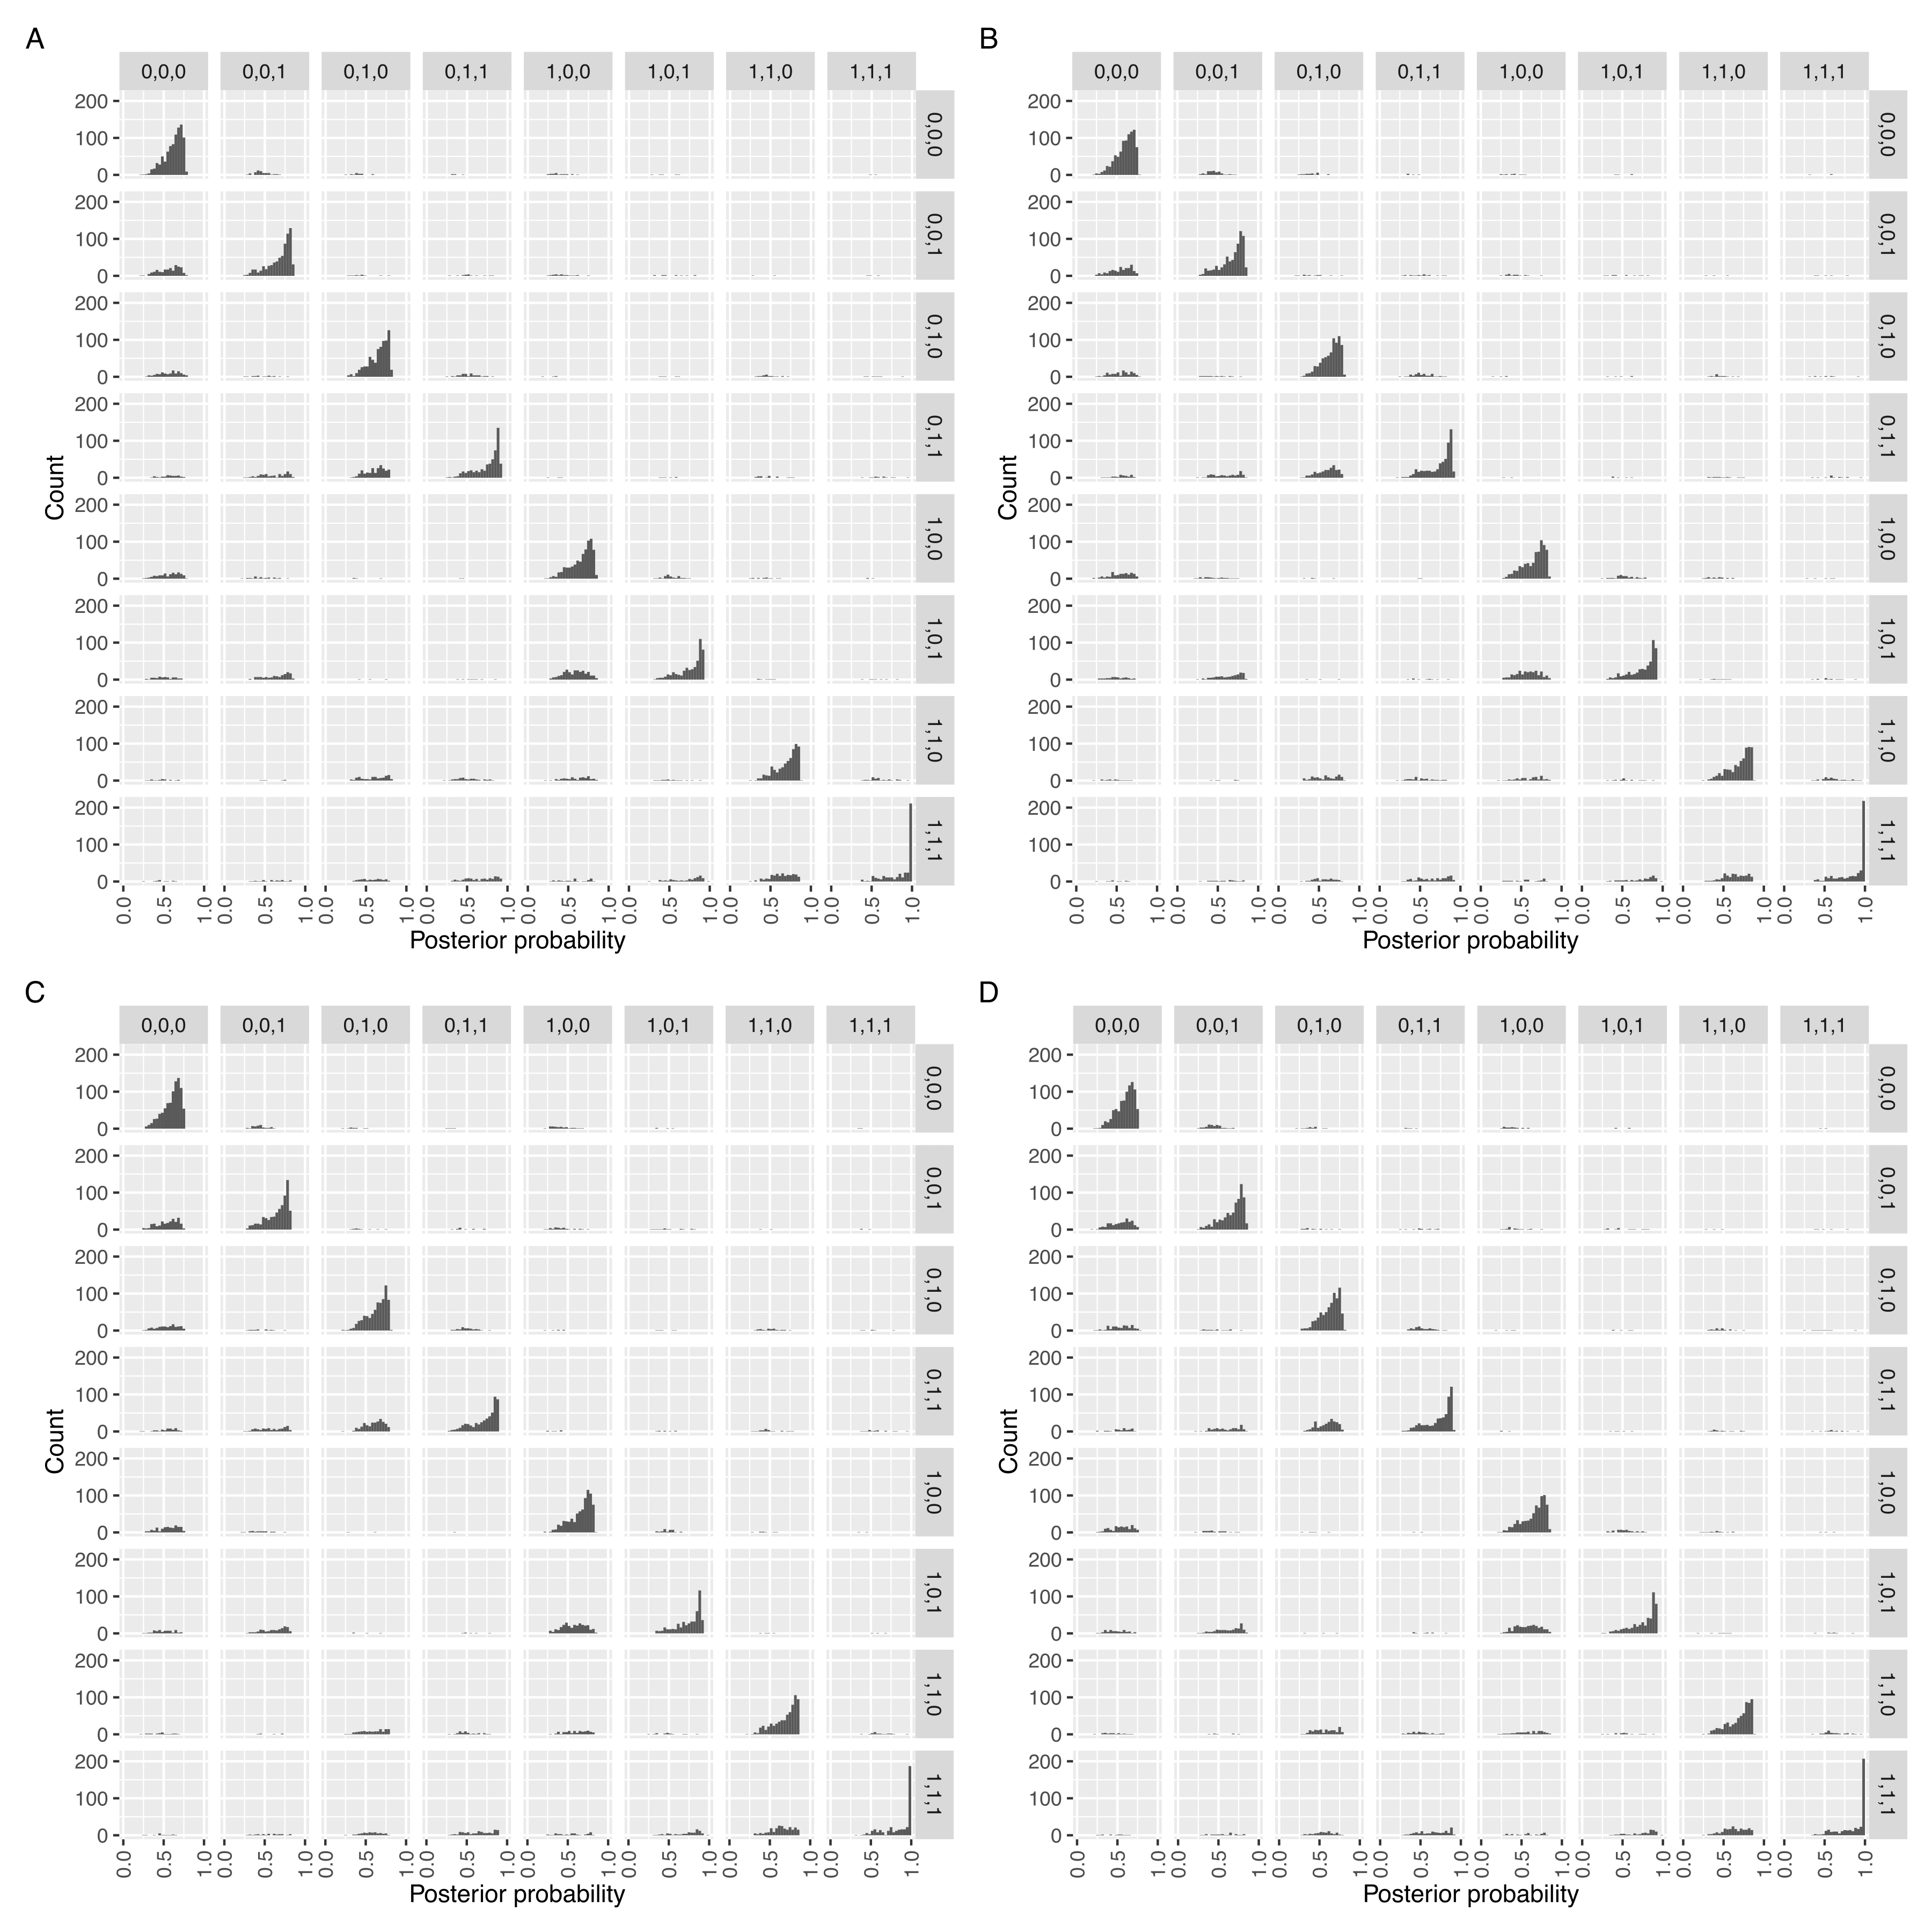
\includegraphics[width=1\textwidth]{png/sim_hist_map_lap_nl.png}
\end{center}  
\caption{
  {\bf
    S4.4 Fig.
    Stratified histograms of posterior probability of the eight models obtained by BMS with $\log$-NL using MAP estimation and Laplace approximation.}
The same as in \sfighistmcmcnl but for MAP estimation and Laplace approximation.
}
\label{s-fig:sim-hist-map-nl}
\end{figure}

\begin{figure}[!ht]
\begin{center}
  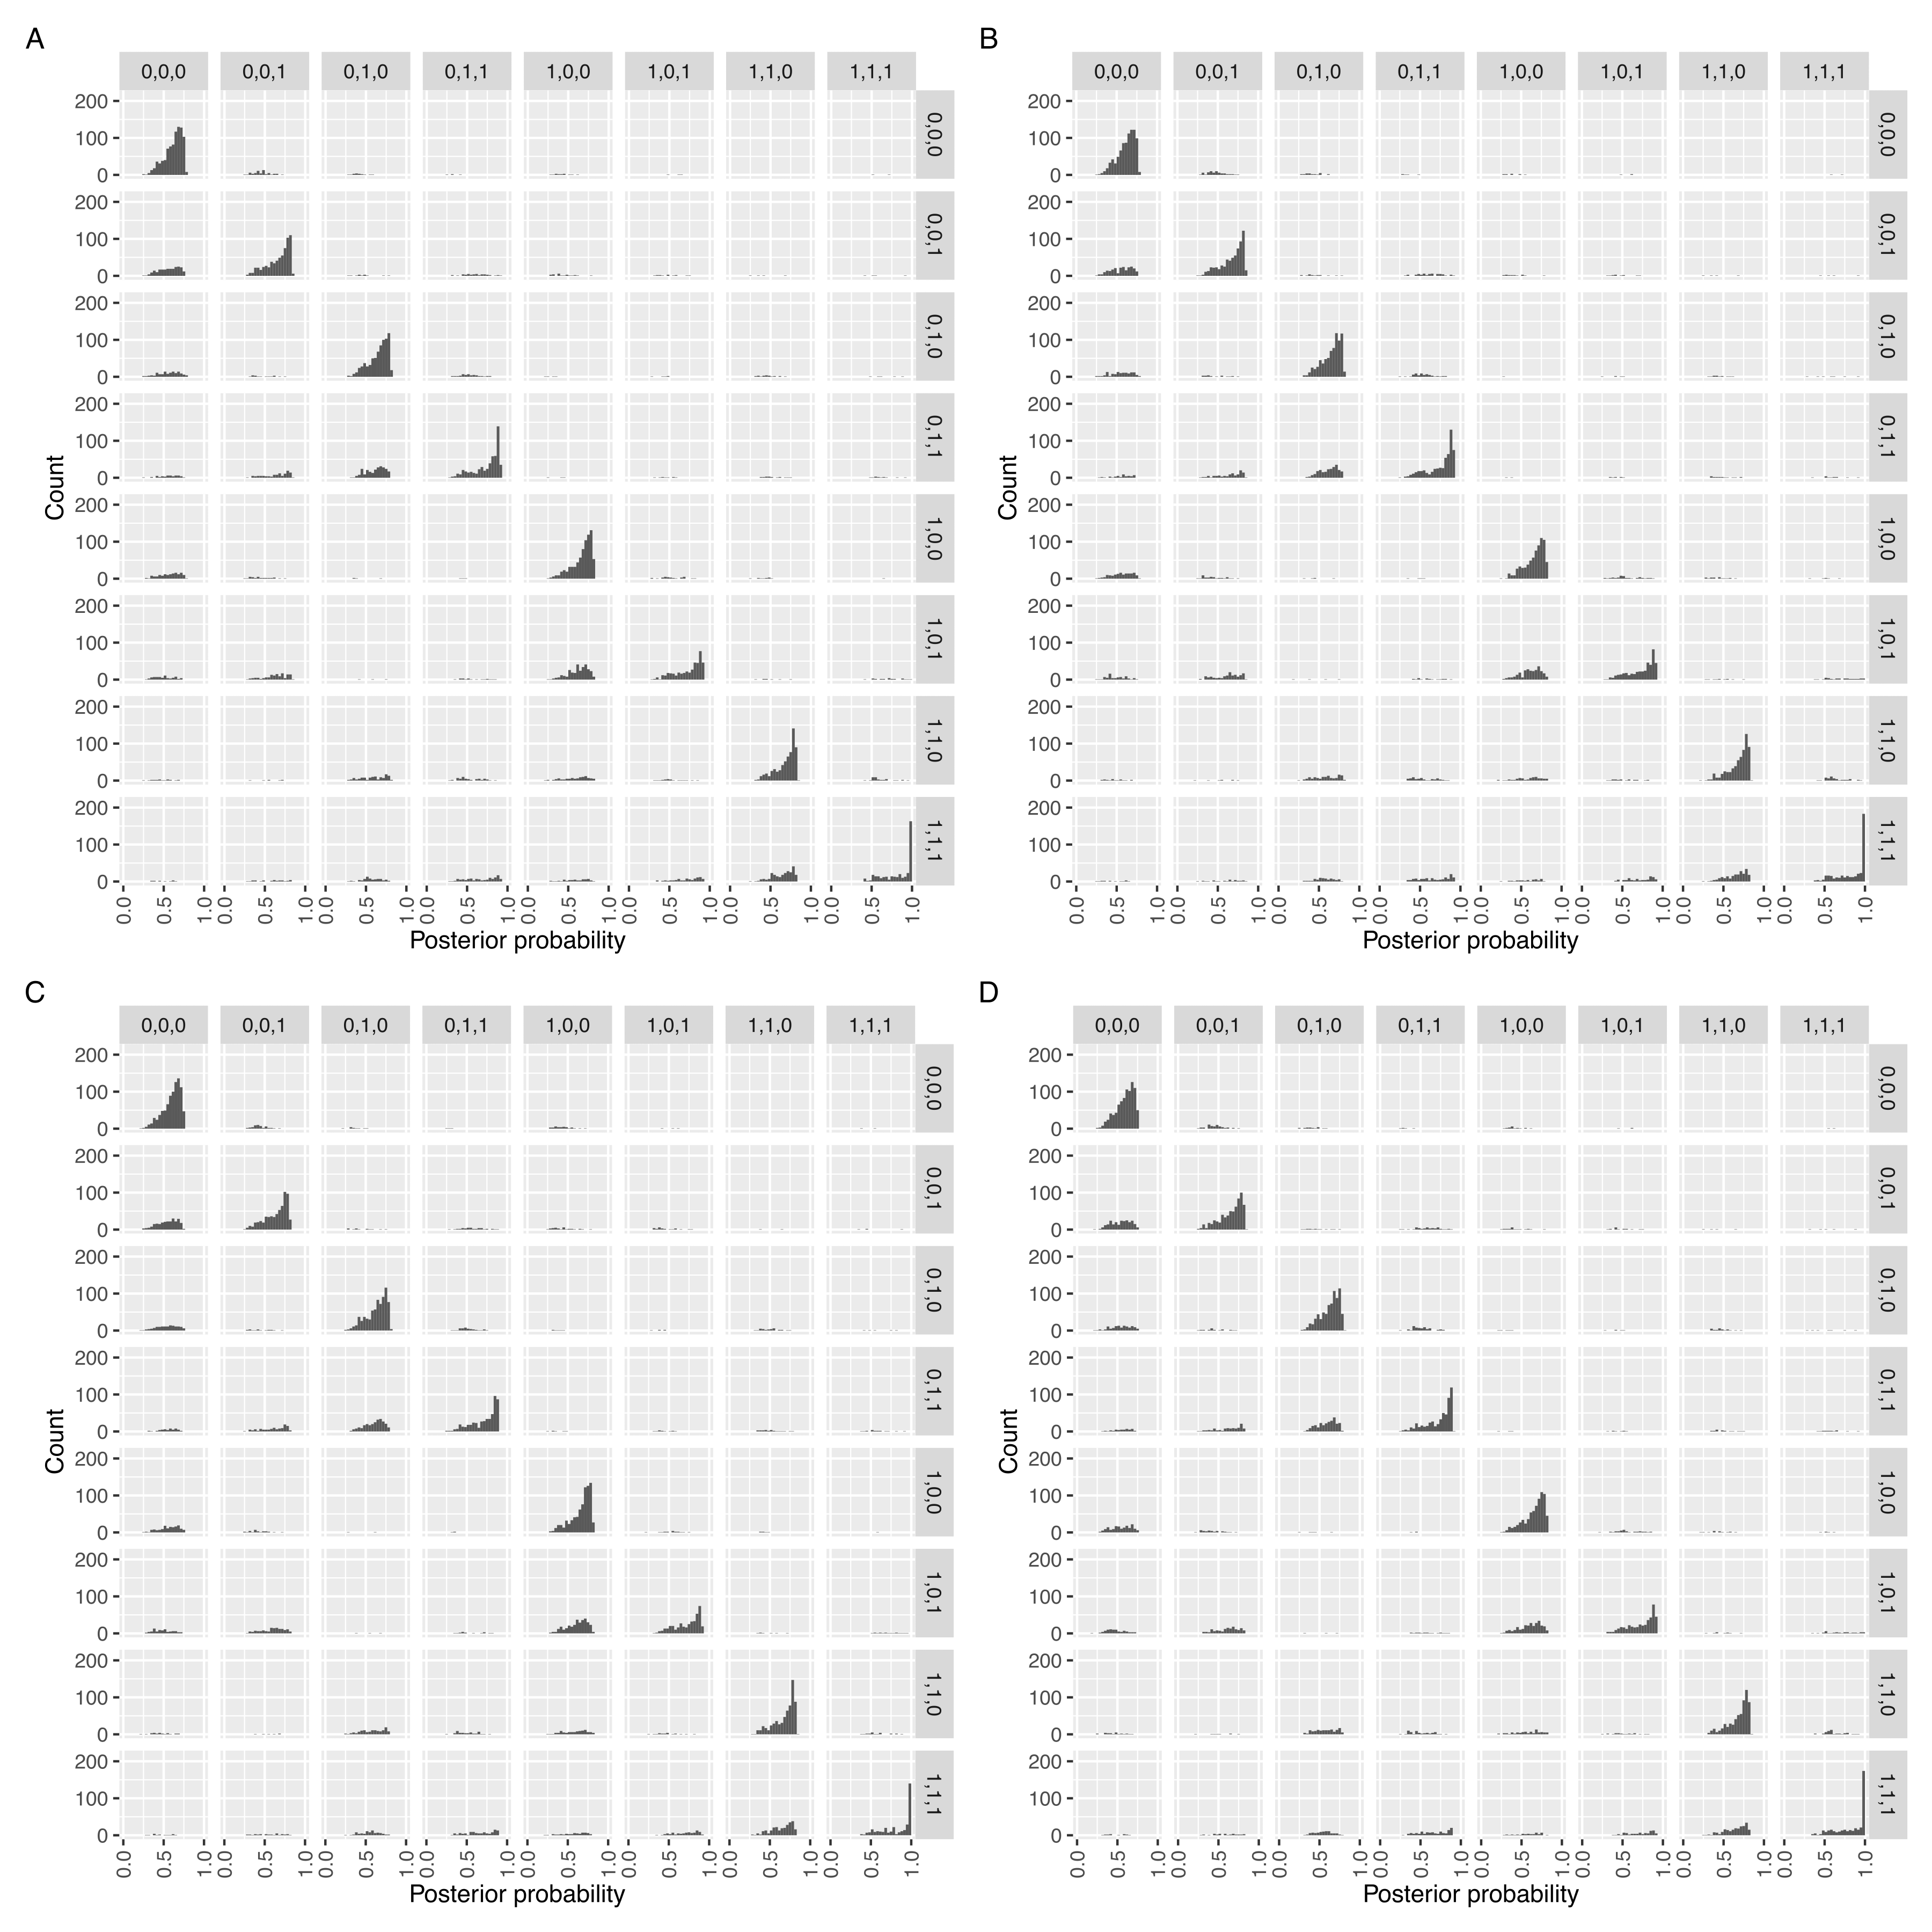
\includegraphics[width=1\textwidth]{png/sim_hist_map_lap_lm.png}
\end{center}  
\caption{
  {\bf
    S4.5 Fig.
    Stratified histograms of posterior probability of the eight models obtained by BMS with $\log$-LM using MAP estimation and Laplace approximation.}
The same as in \sfighistmapnl but for $\log$-LM.
}
\label{s-fig:sim-hist-map-lm}
\end{figure}

\begin{figure}[!ht]
\begin{center}
  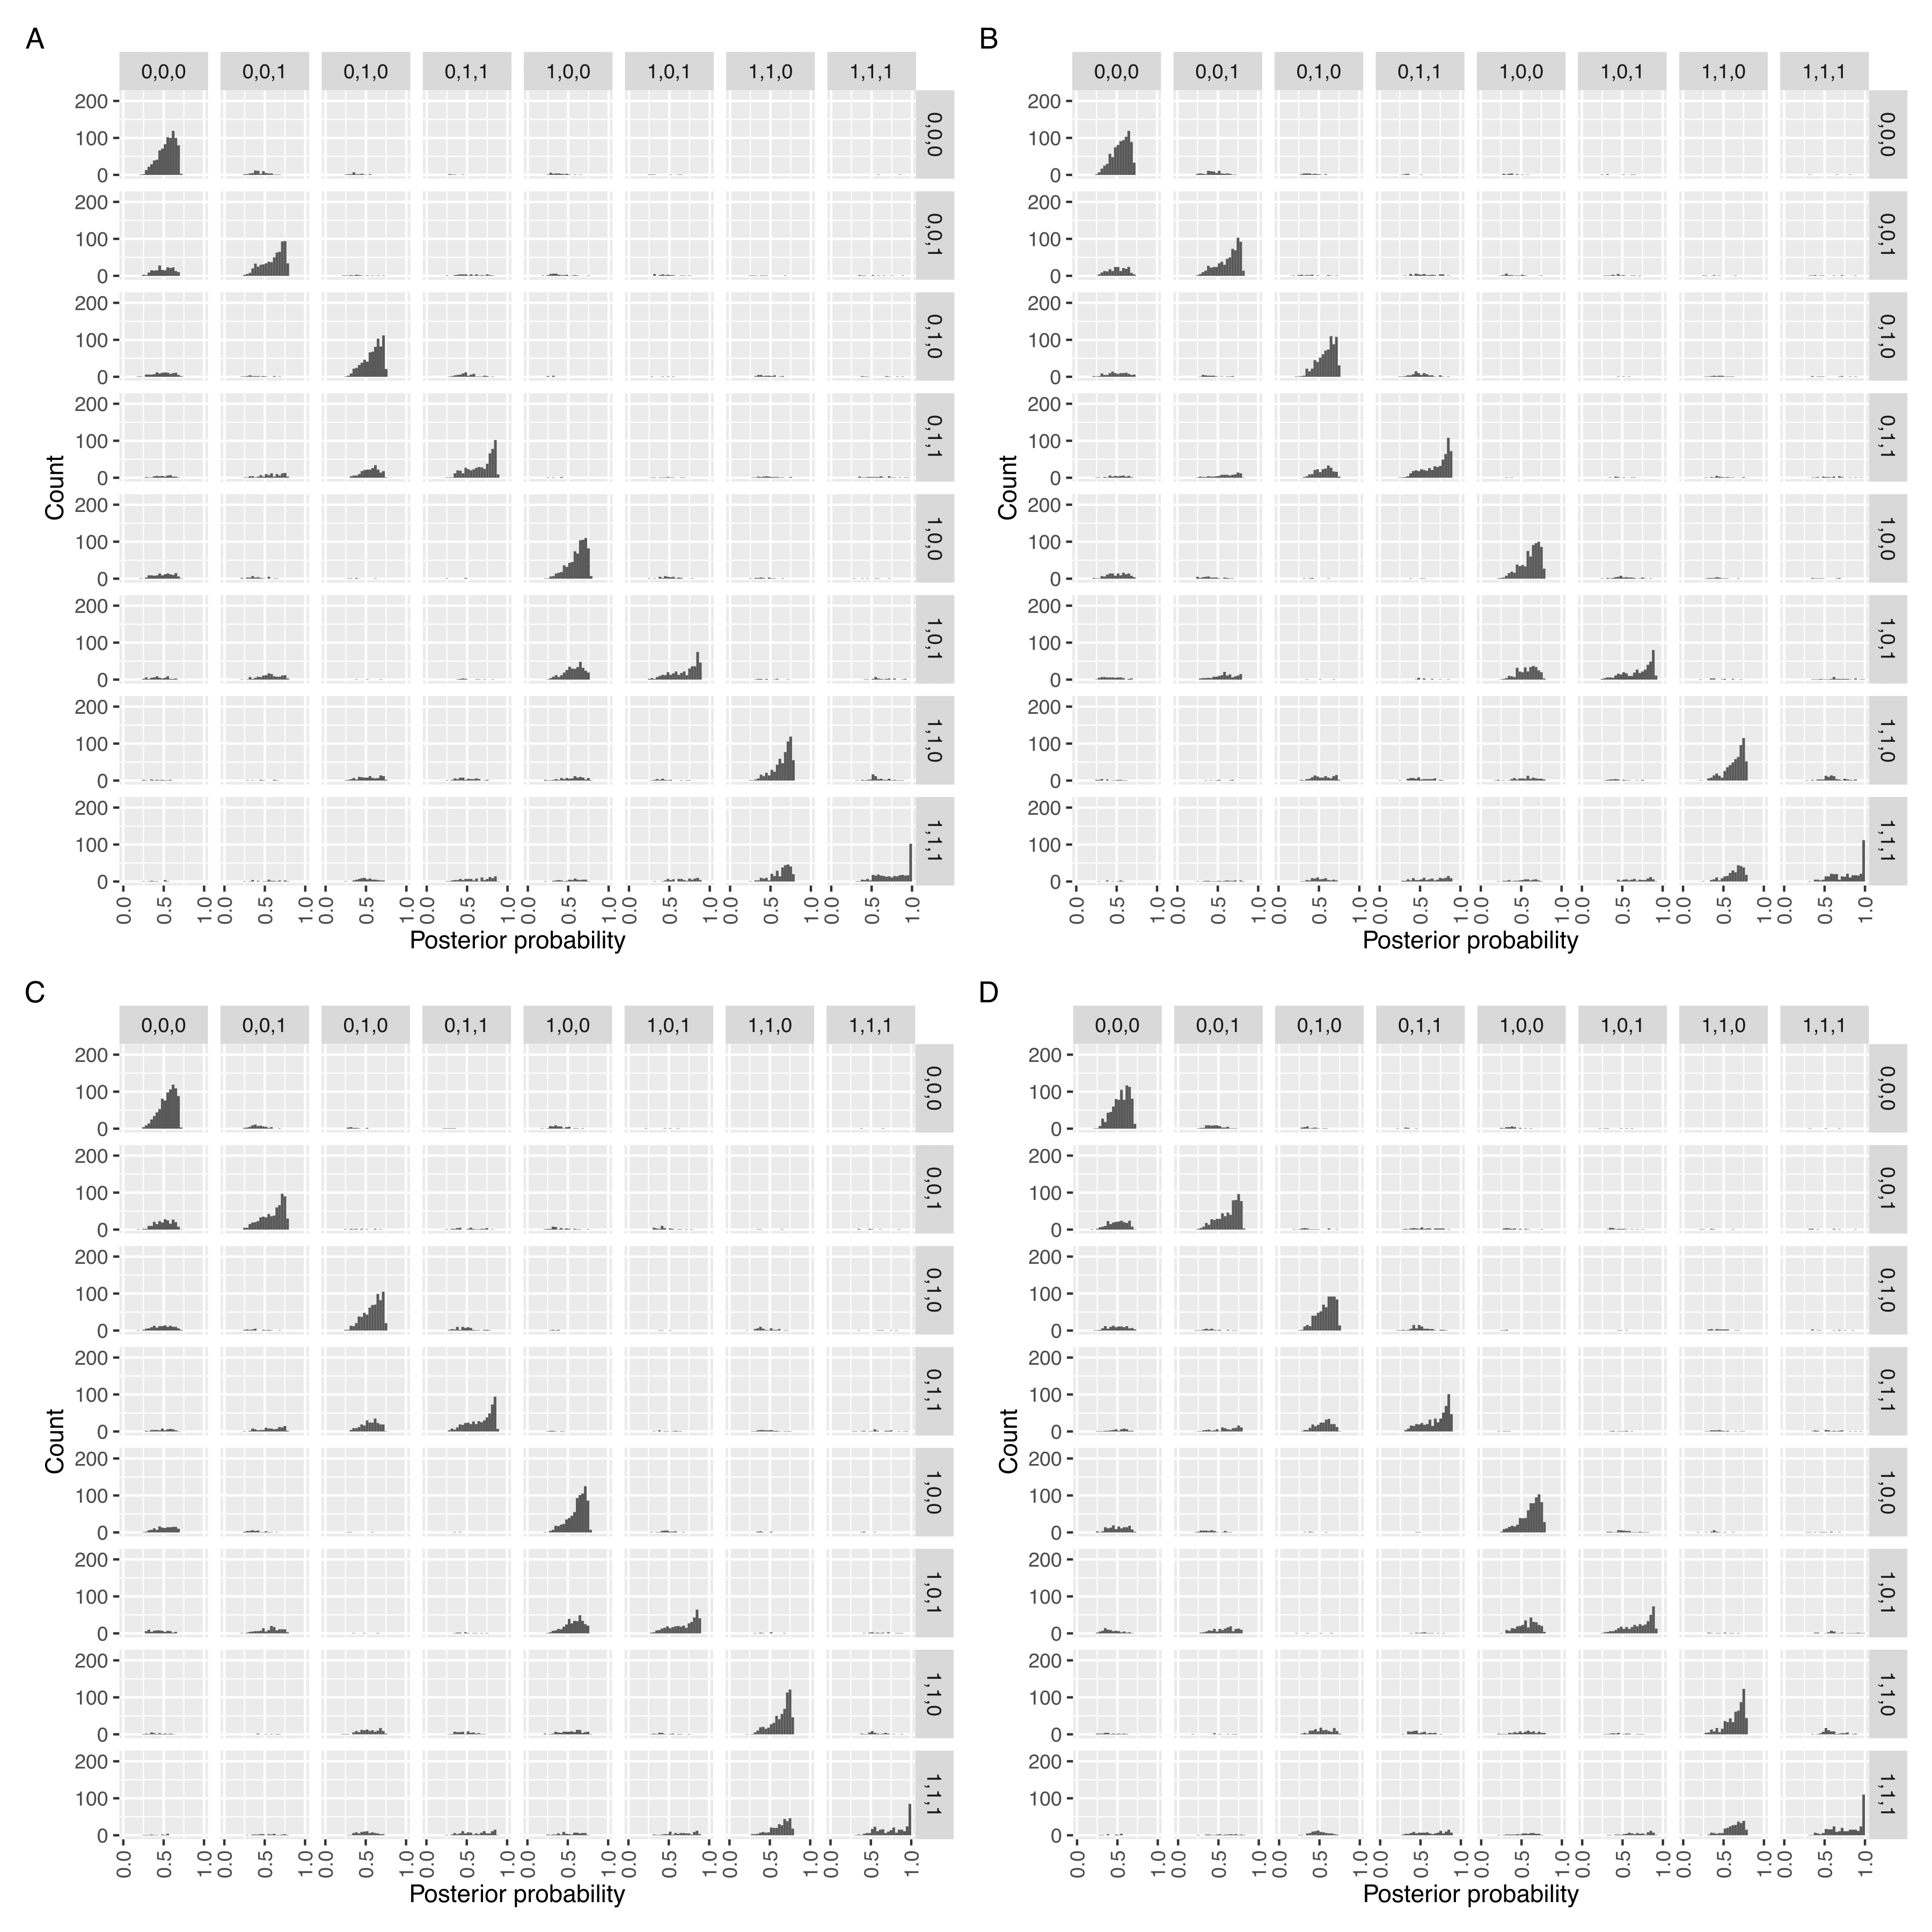
\includegraphics[width=1\textwidth]{png/sim_hist_map_lap_rint.png}
\end{center}  
\caption{
  {\bf
    S4.6 Fig.
    Stratified histograms of posterior probability of the eight models obtained by BMS wth RINT-LM using MAP estimation and Laplace approximation.}
The same as in \sfighistmapnl but for RINT-LM.
}
\label{s-fig:sim-hist-map-rint}
\end{figure}

\begin{figure}[!ht]
\begin{center}
  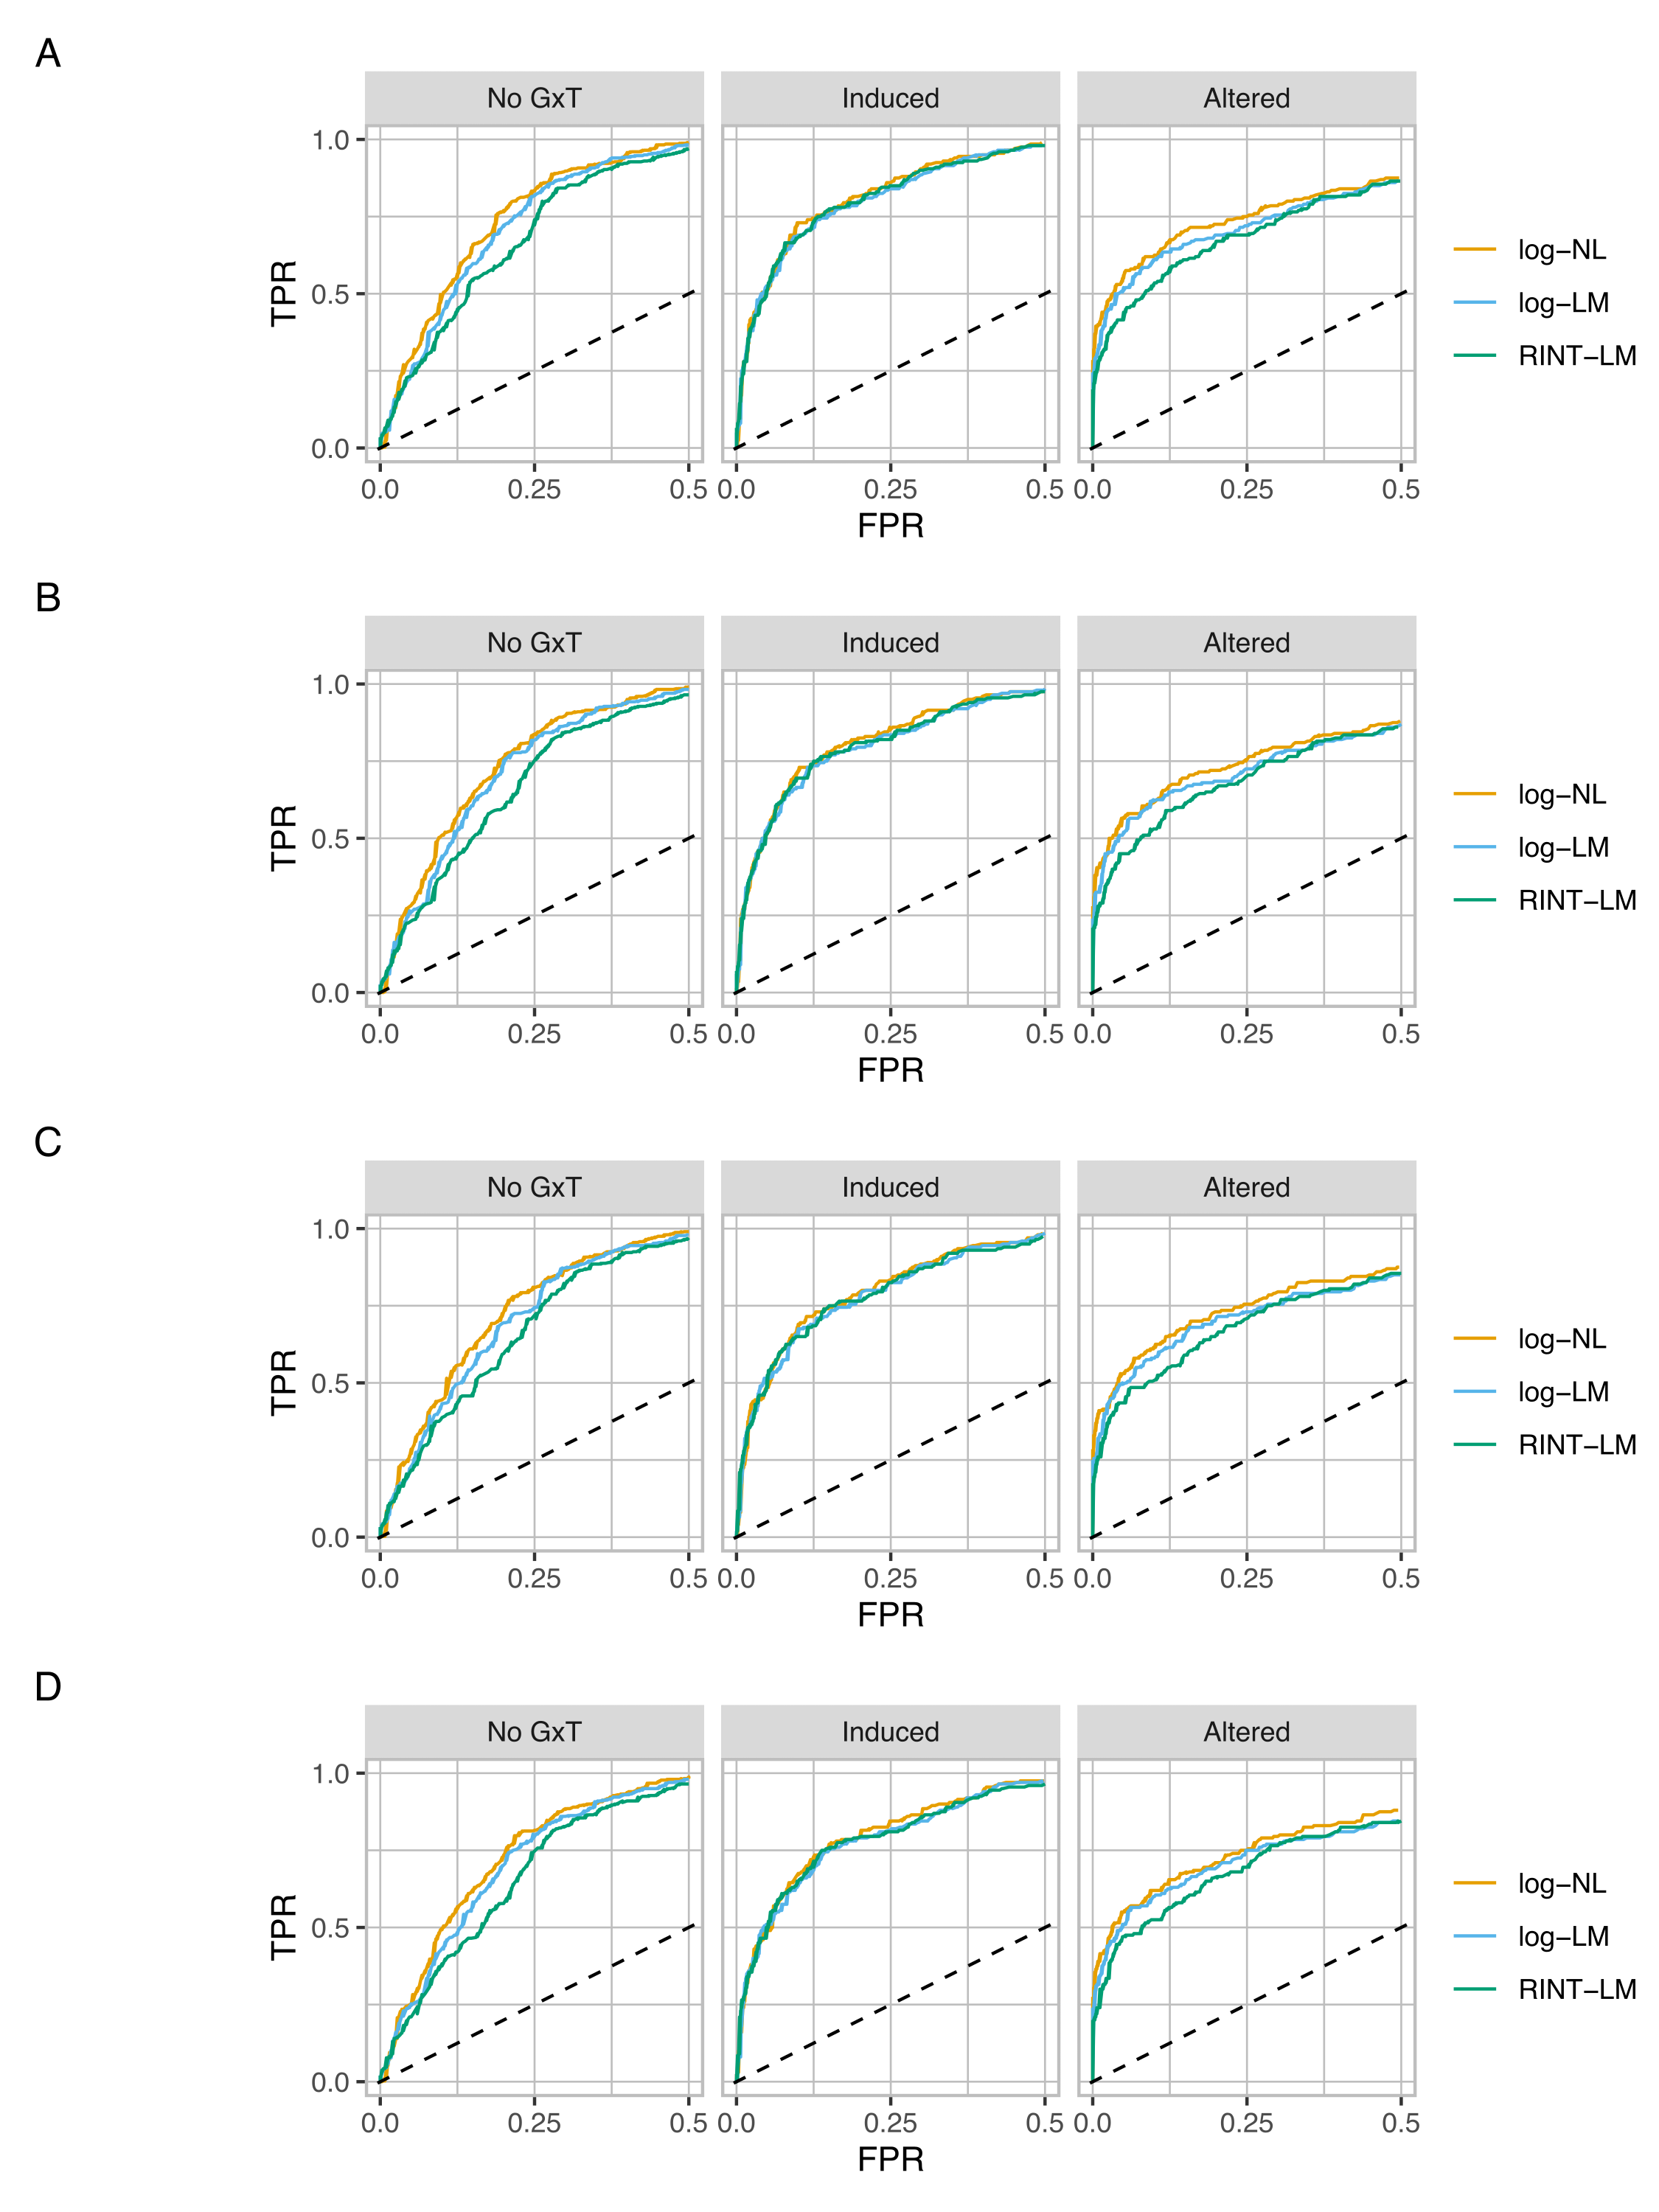
\includegraphics[width=0.8\textwidth]{png/sim_procc_mcmc_bs.png}
\end{center}
\caption{
  {\bf
    S5 Fig.
    Partial ROC curves assessing the performance of BMS with $\log$-NL, $\log$-LM, and RINT-LM for the no-\GxT, induced, and altered categories using MCMC and bridge sampling.}
The panels \textbf{A} to \textbf{D} show the results in scenarios 1 to 4, which are described in the legend to \sfigroccmcmc.
}
\label{s-fig:sim-procc-mcmc}
\end{figure}

\begin{figure}[!ht]
\begin{center}
  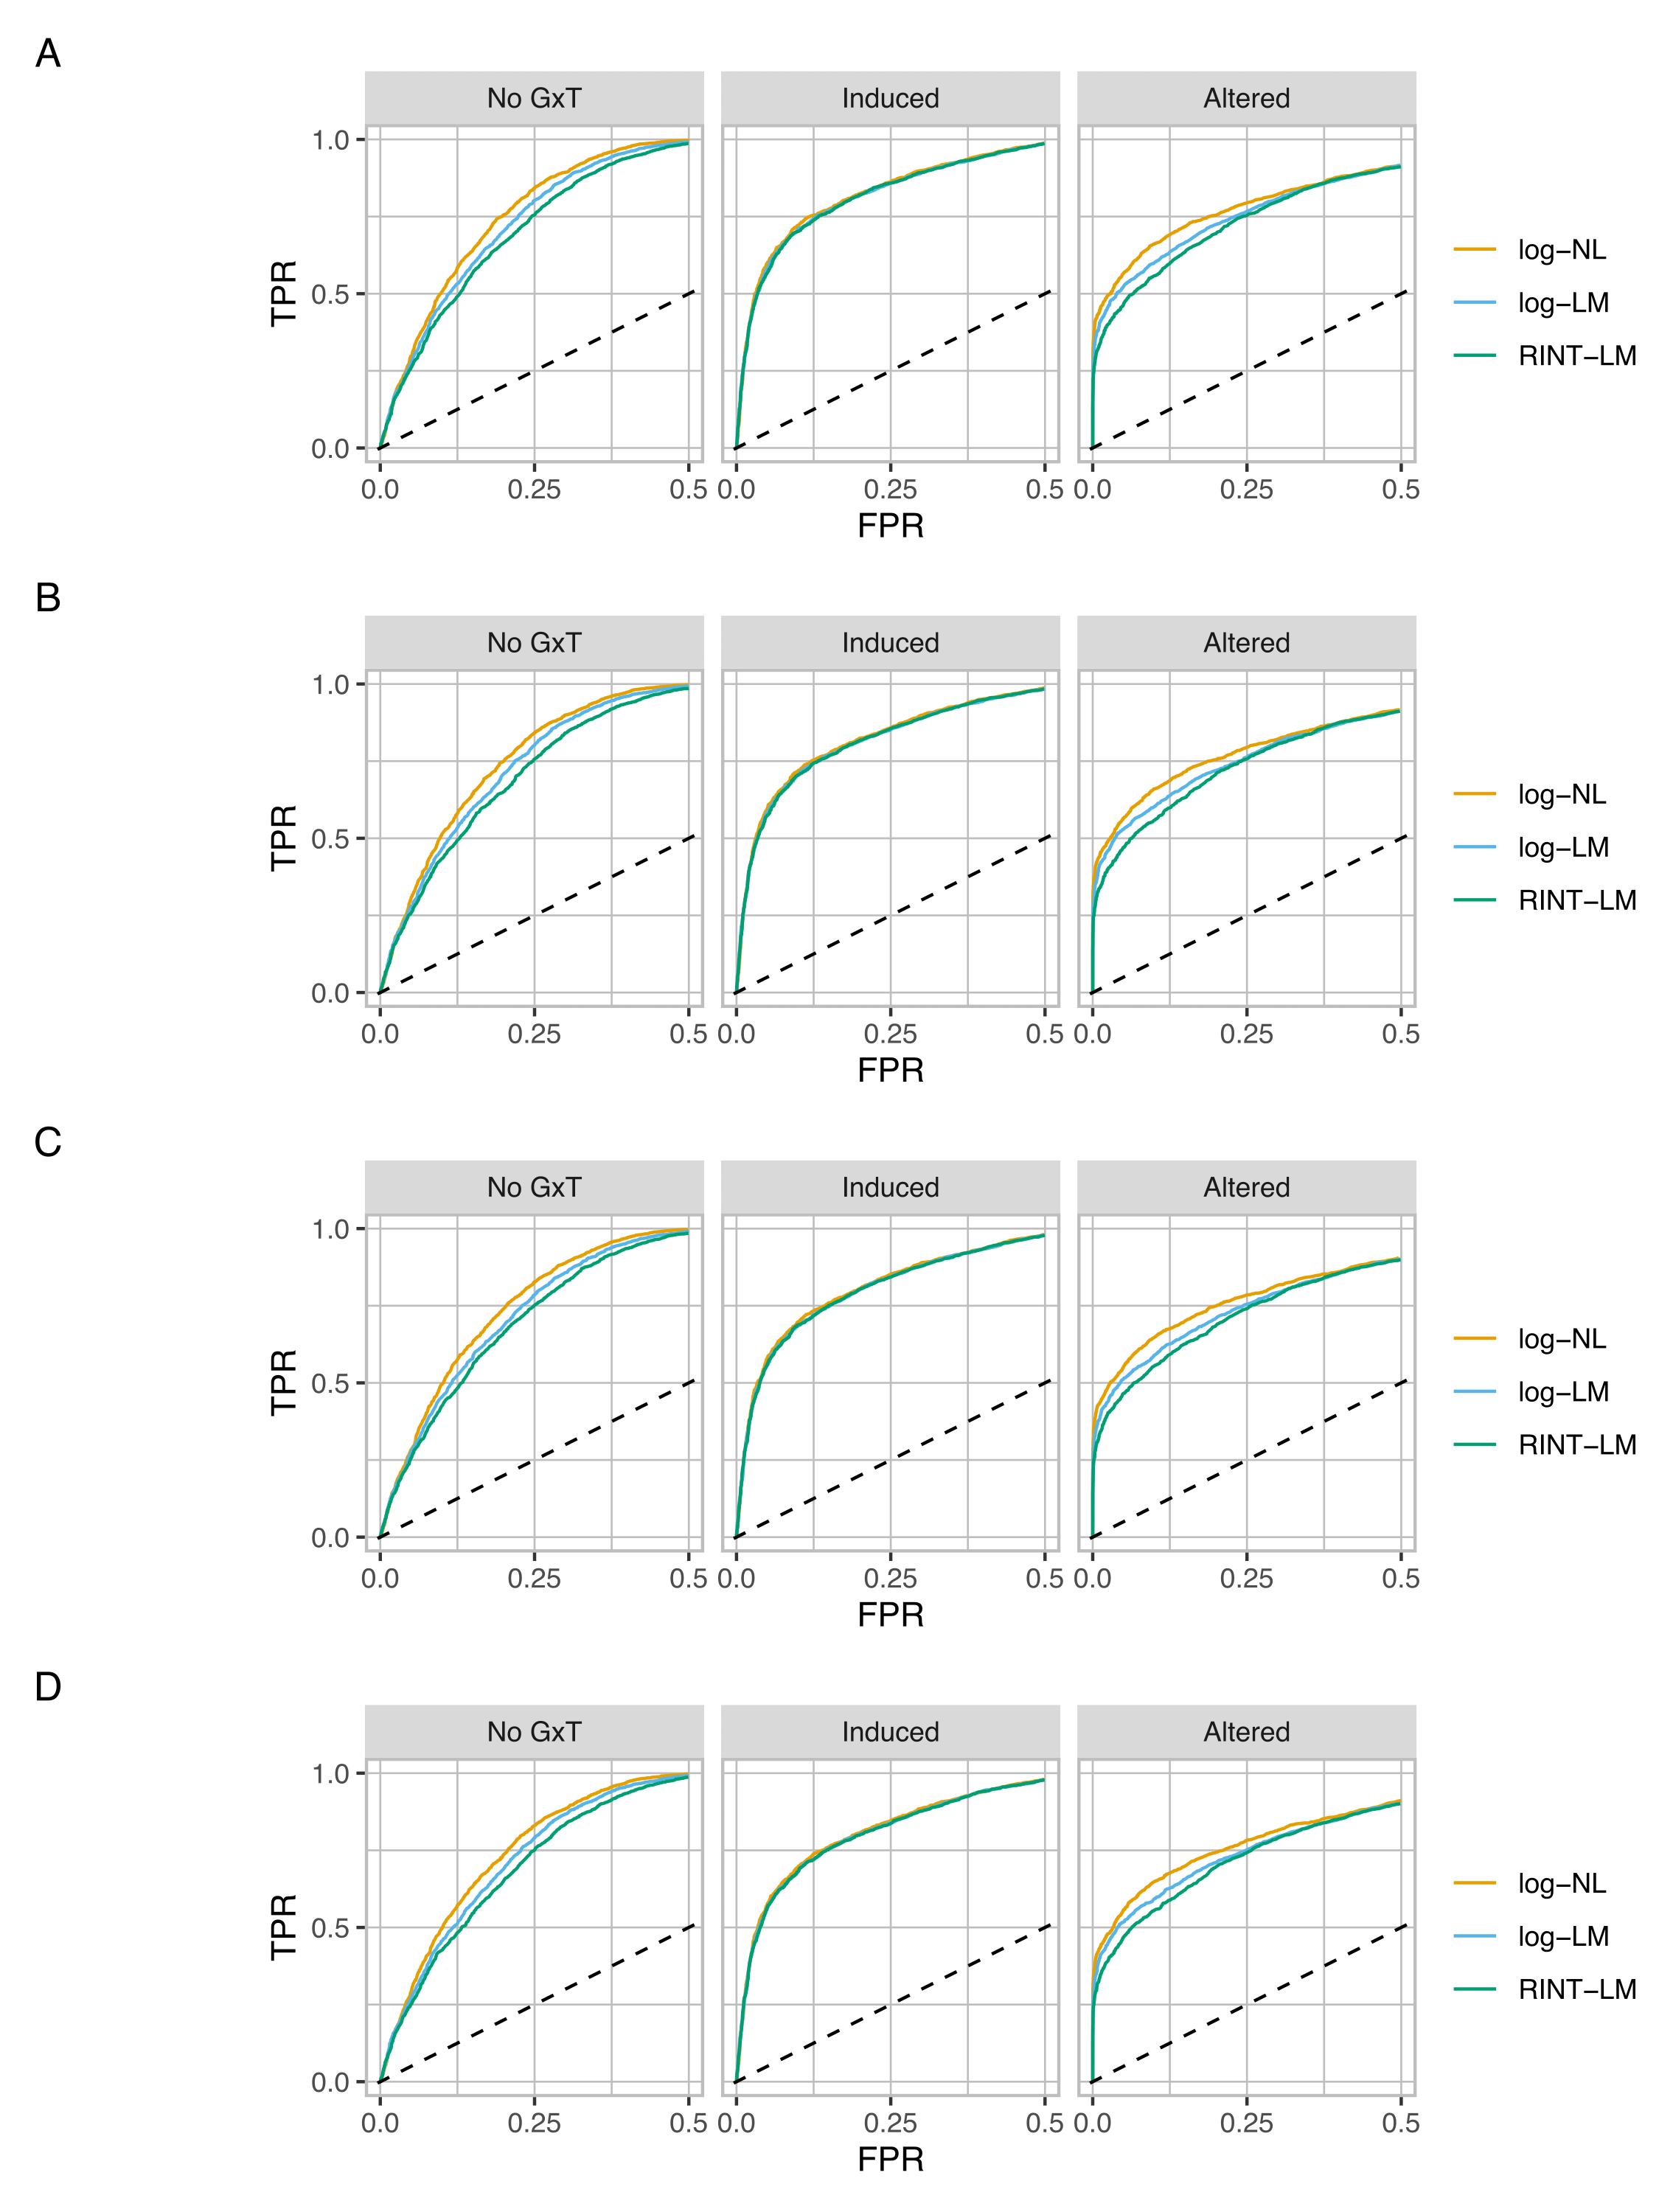
\includegraphics[width=0.8\textwidth]{png/sim_procc_map_lap.png}
\end{center}  
\caption{
  {\bf
    S5.2 Fig.
    Partial ROC curves assessing the performance of BMS with $\log$-NL, $\log$-LM, and RINT-LM for the no-\GxT, induced, and altered categories using MAP and Laplace approximation.}
The panels \textbf{A} to \textbf{D} show the results in scenarios 1 to 4, which are described in the legend to \sfigroccmcmc.
}
\label{s-fig:sim-procc-map}
\end{figure}

\begin{figure}[!ht]
\begin{center}
  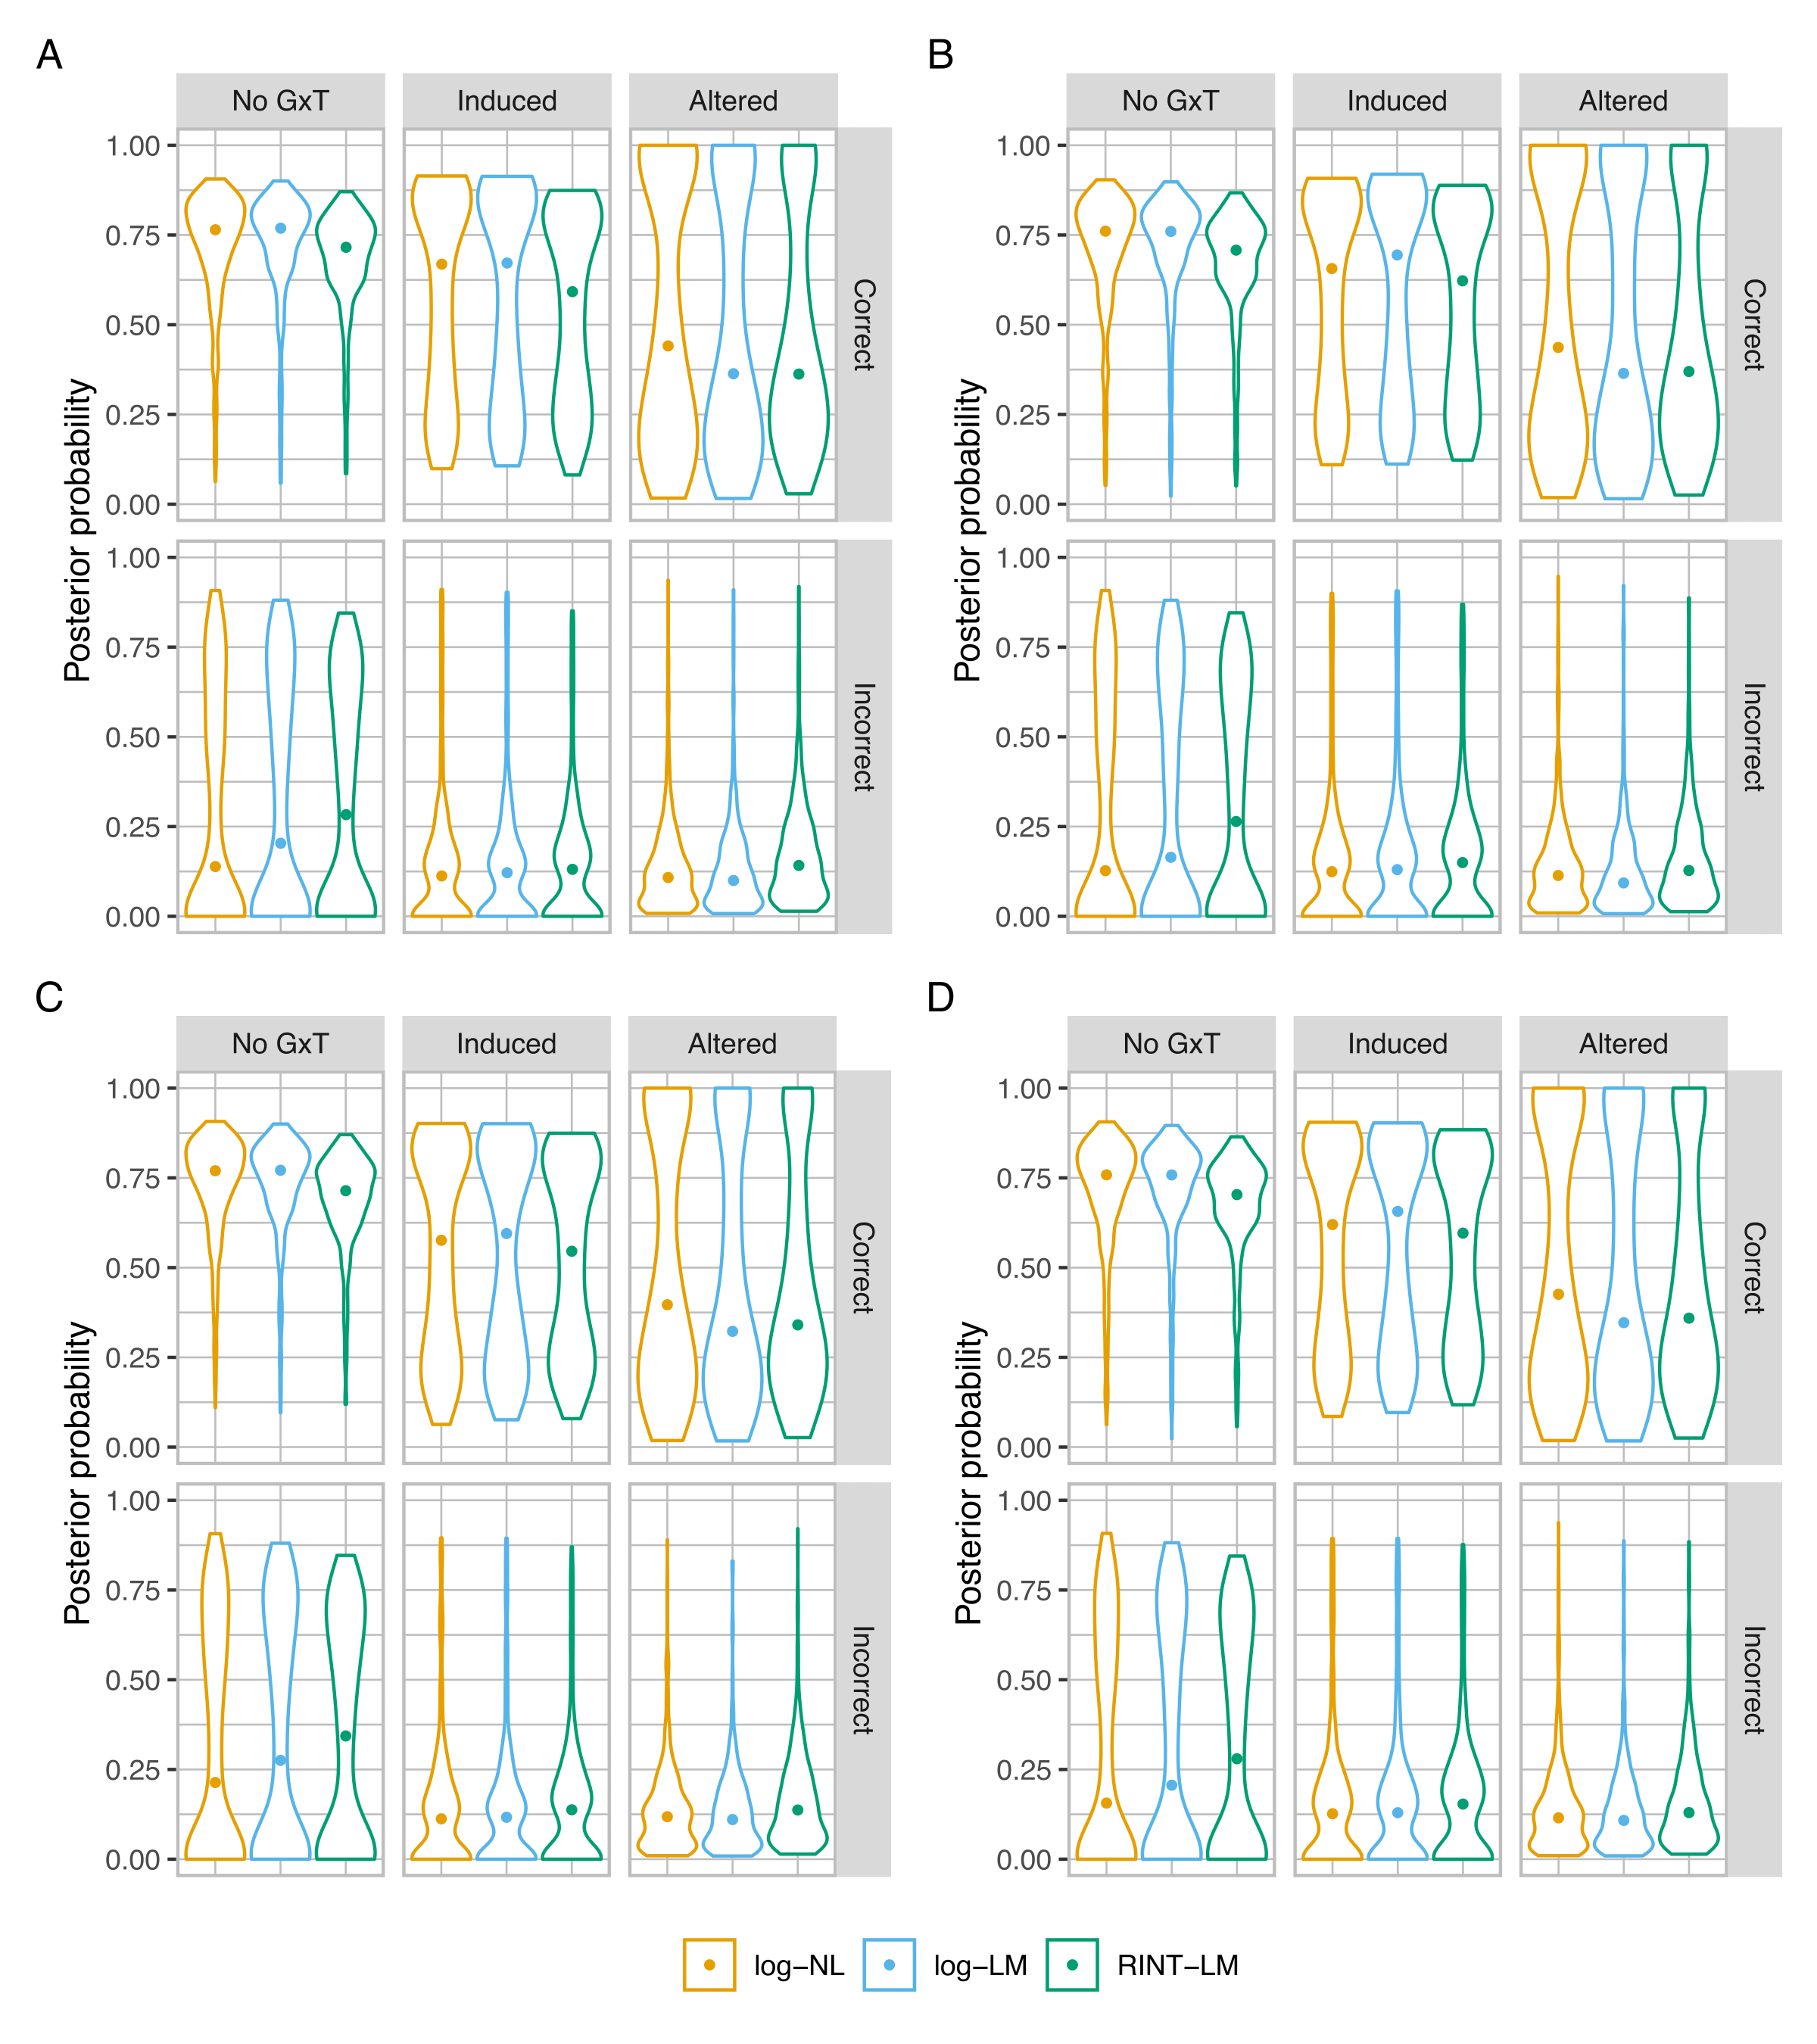
\includegraphics[width=0.9\textwidth]{png/sim_vln_aggr_mcmc_bs.png}
\end{center}  
\caption{
  {\bf
    S6 Fig.
    Posterior probability of the correct and incorrect models for aggregated categories obtained by BMS using MCMC and bridge sampling.}
Violin plots for comparing the performance of BMS with $\log$-NL, $\log$-LM, and RINT-LM based on the distribution of posterior probability of the correct and incorrect models for the ``no GxT'', ``induced'', and ``altered'' model categories. The closed circles represent median values. The panels \textbf{A} to \textbf{D} show the results in scenarios 1 to 4, which are described in the legend to \sfigroccmcmc.
}
\label{s-fig:sim-vln-aggr-mcmc}
\end{figure}

\begin{figure}[!ht]
\begin{center}
  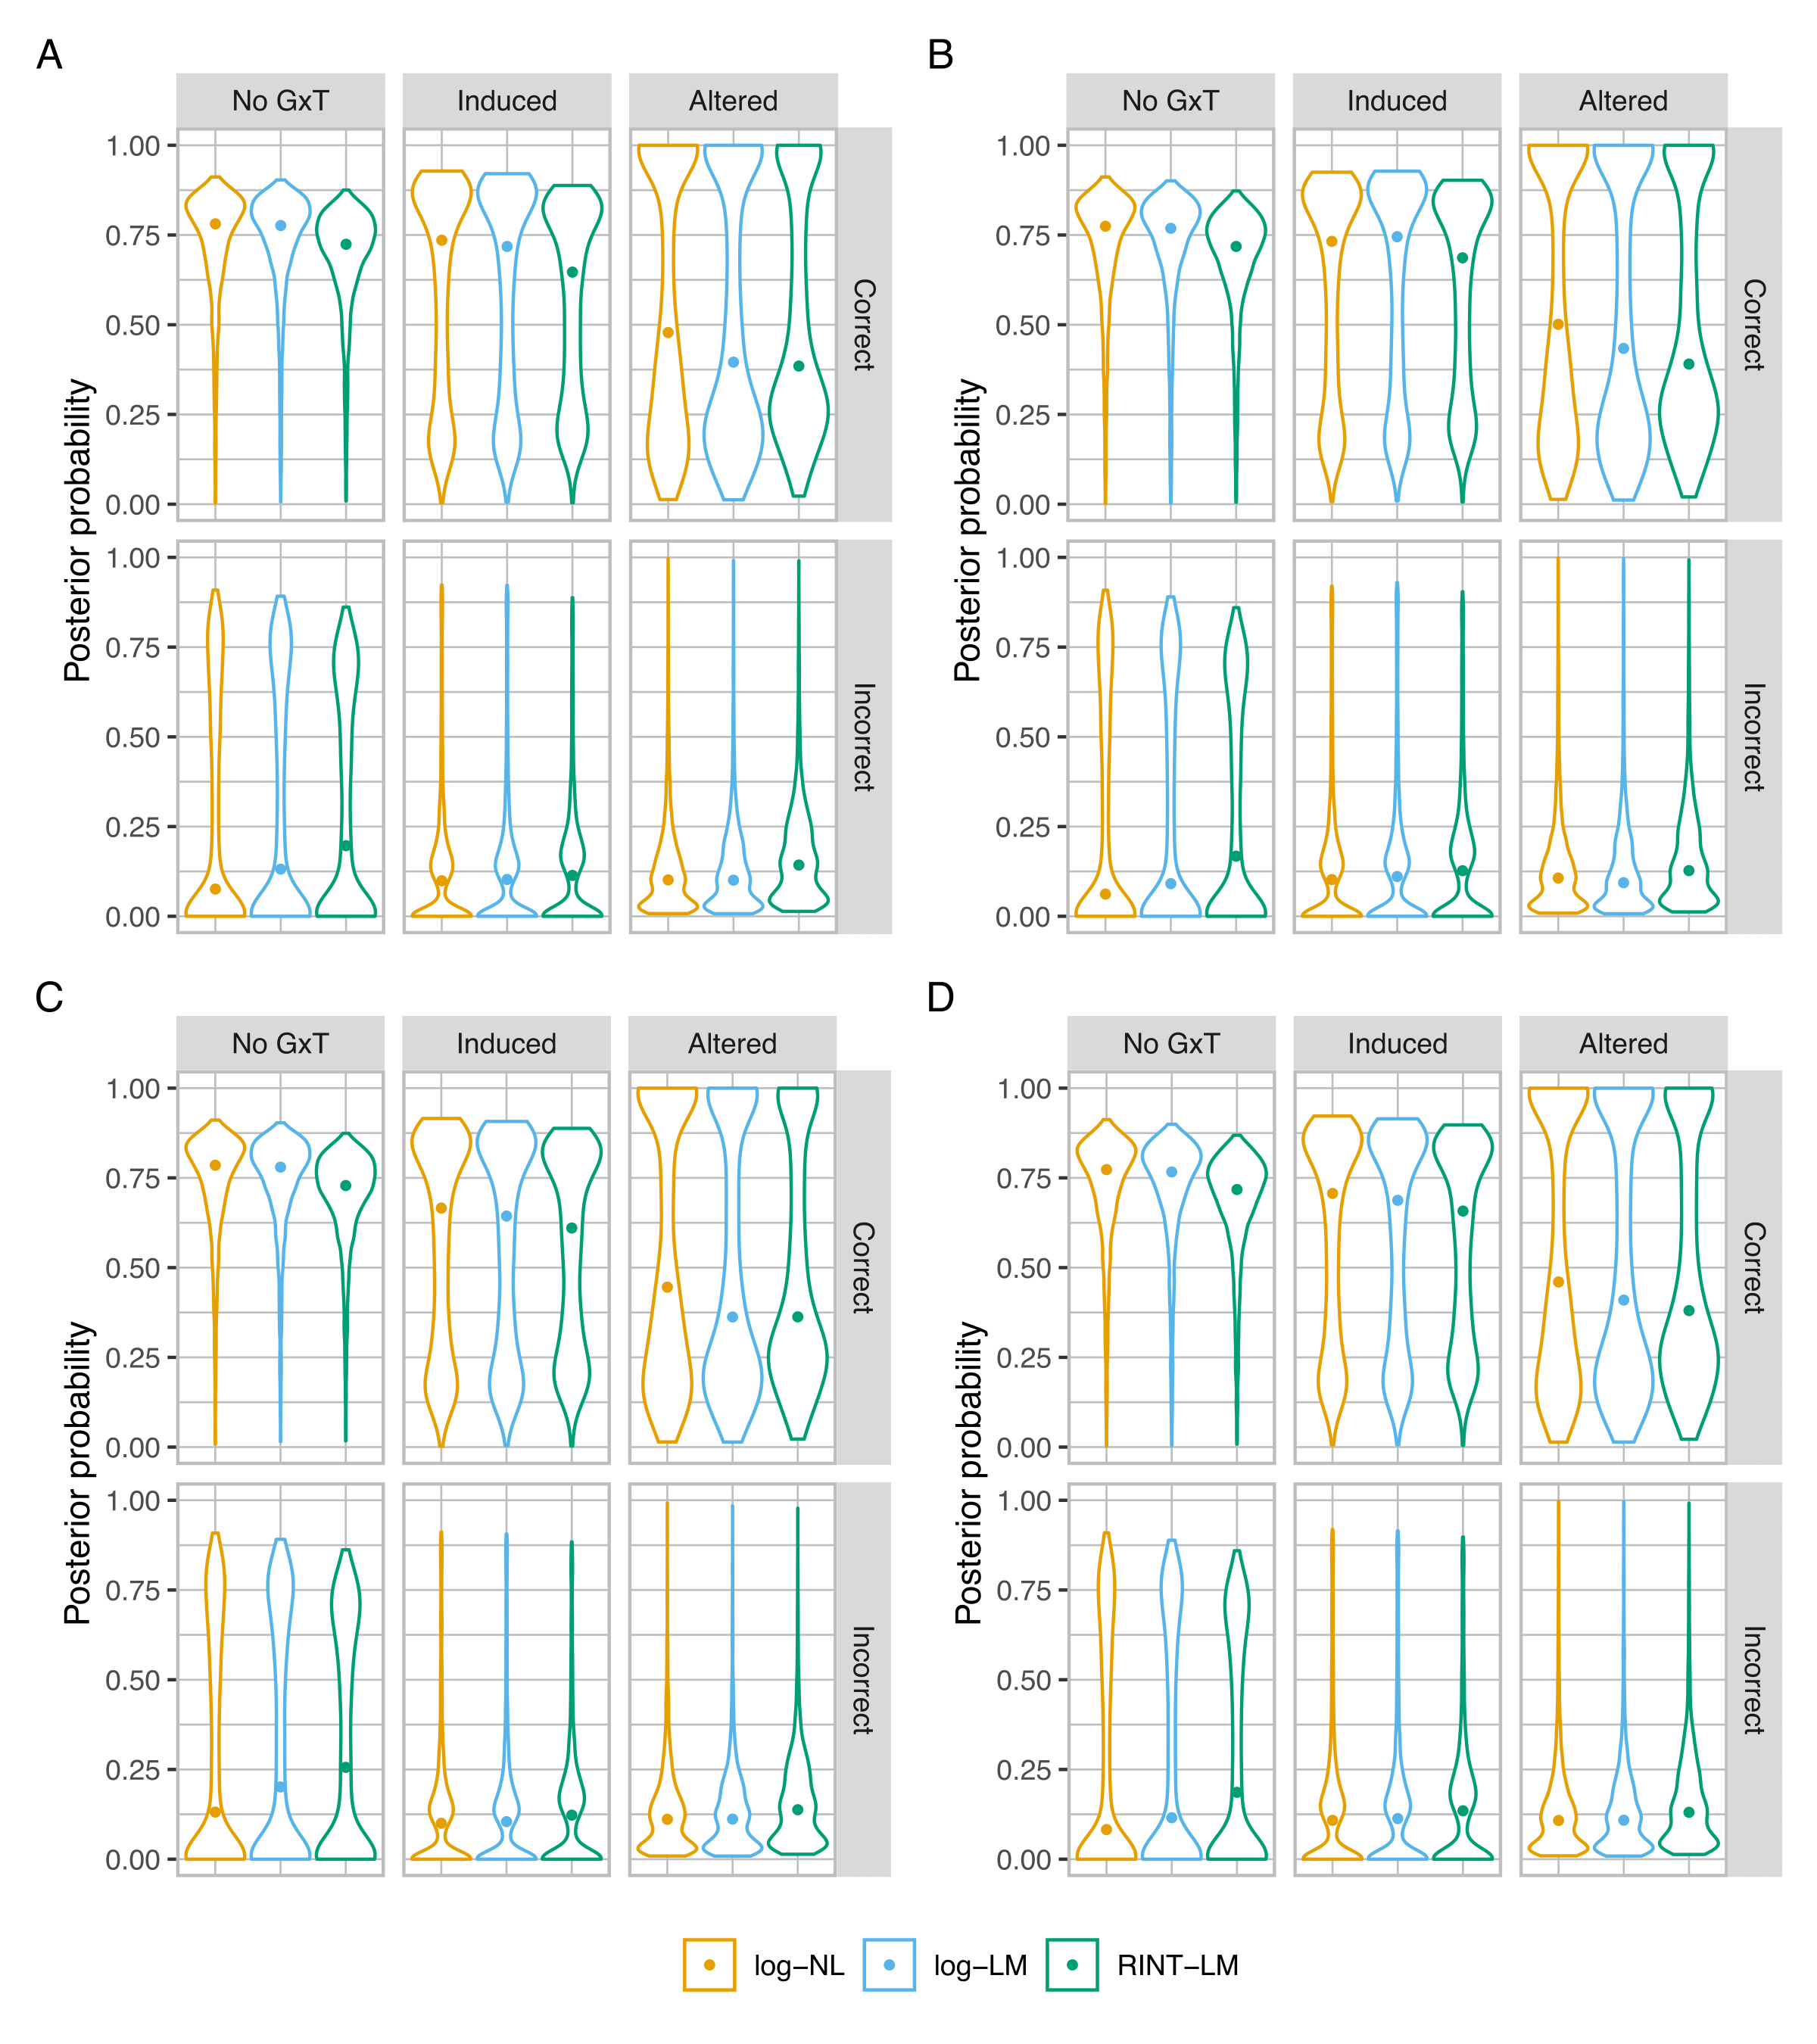
\includegraphics[width=0.9\textwidth]{png/sim_vln_aggr_map_lap.png}
\end{center}  
\caption{
  {\bf
    S6.2 Fig.
    Posterior probability of the correct and incorrect models for aggregated categories obtained by BMS using MAP estimation and Laplace approximation.}
The same as in \sfigppaggrmcmc but for MAP estimation and Laplace approximation.
}
\label{s-fig:sim-vln-aggr-map}
\end{figure}

\begin{figure}[!ht]
\begin{center}
  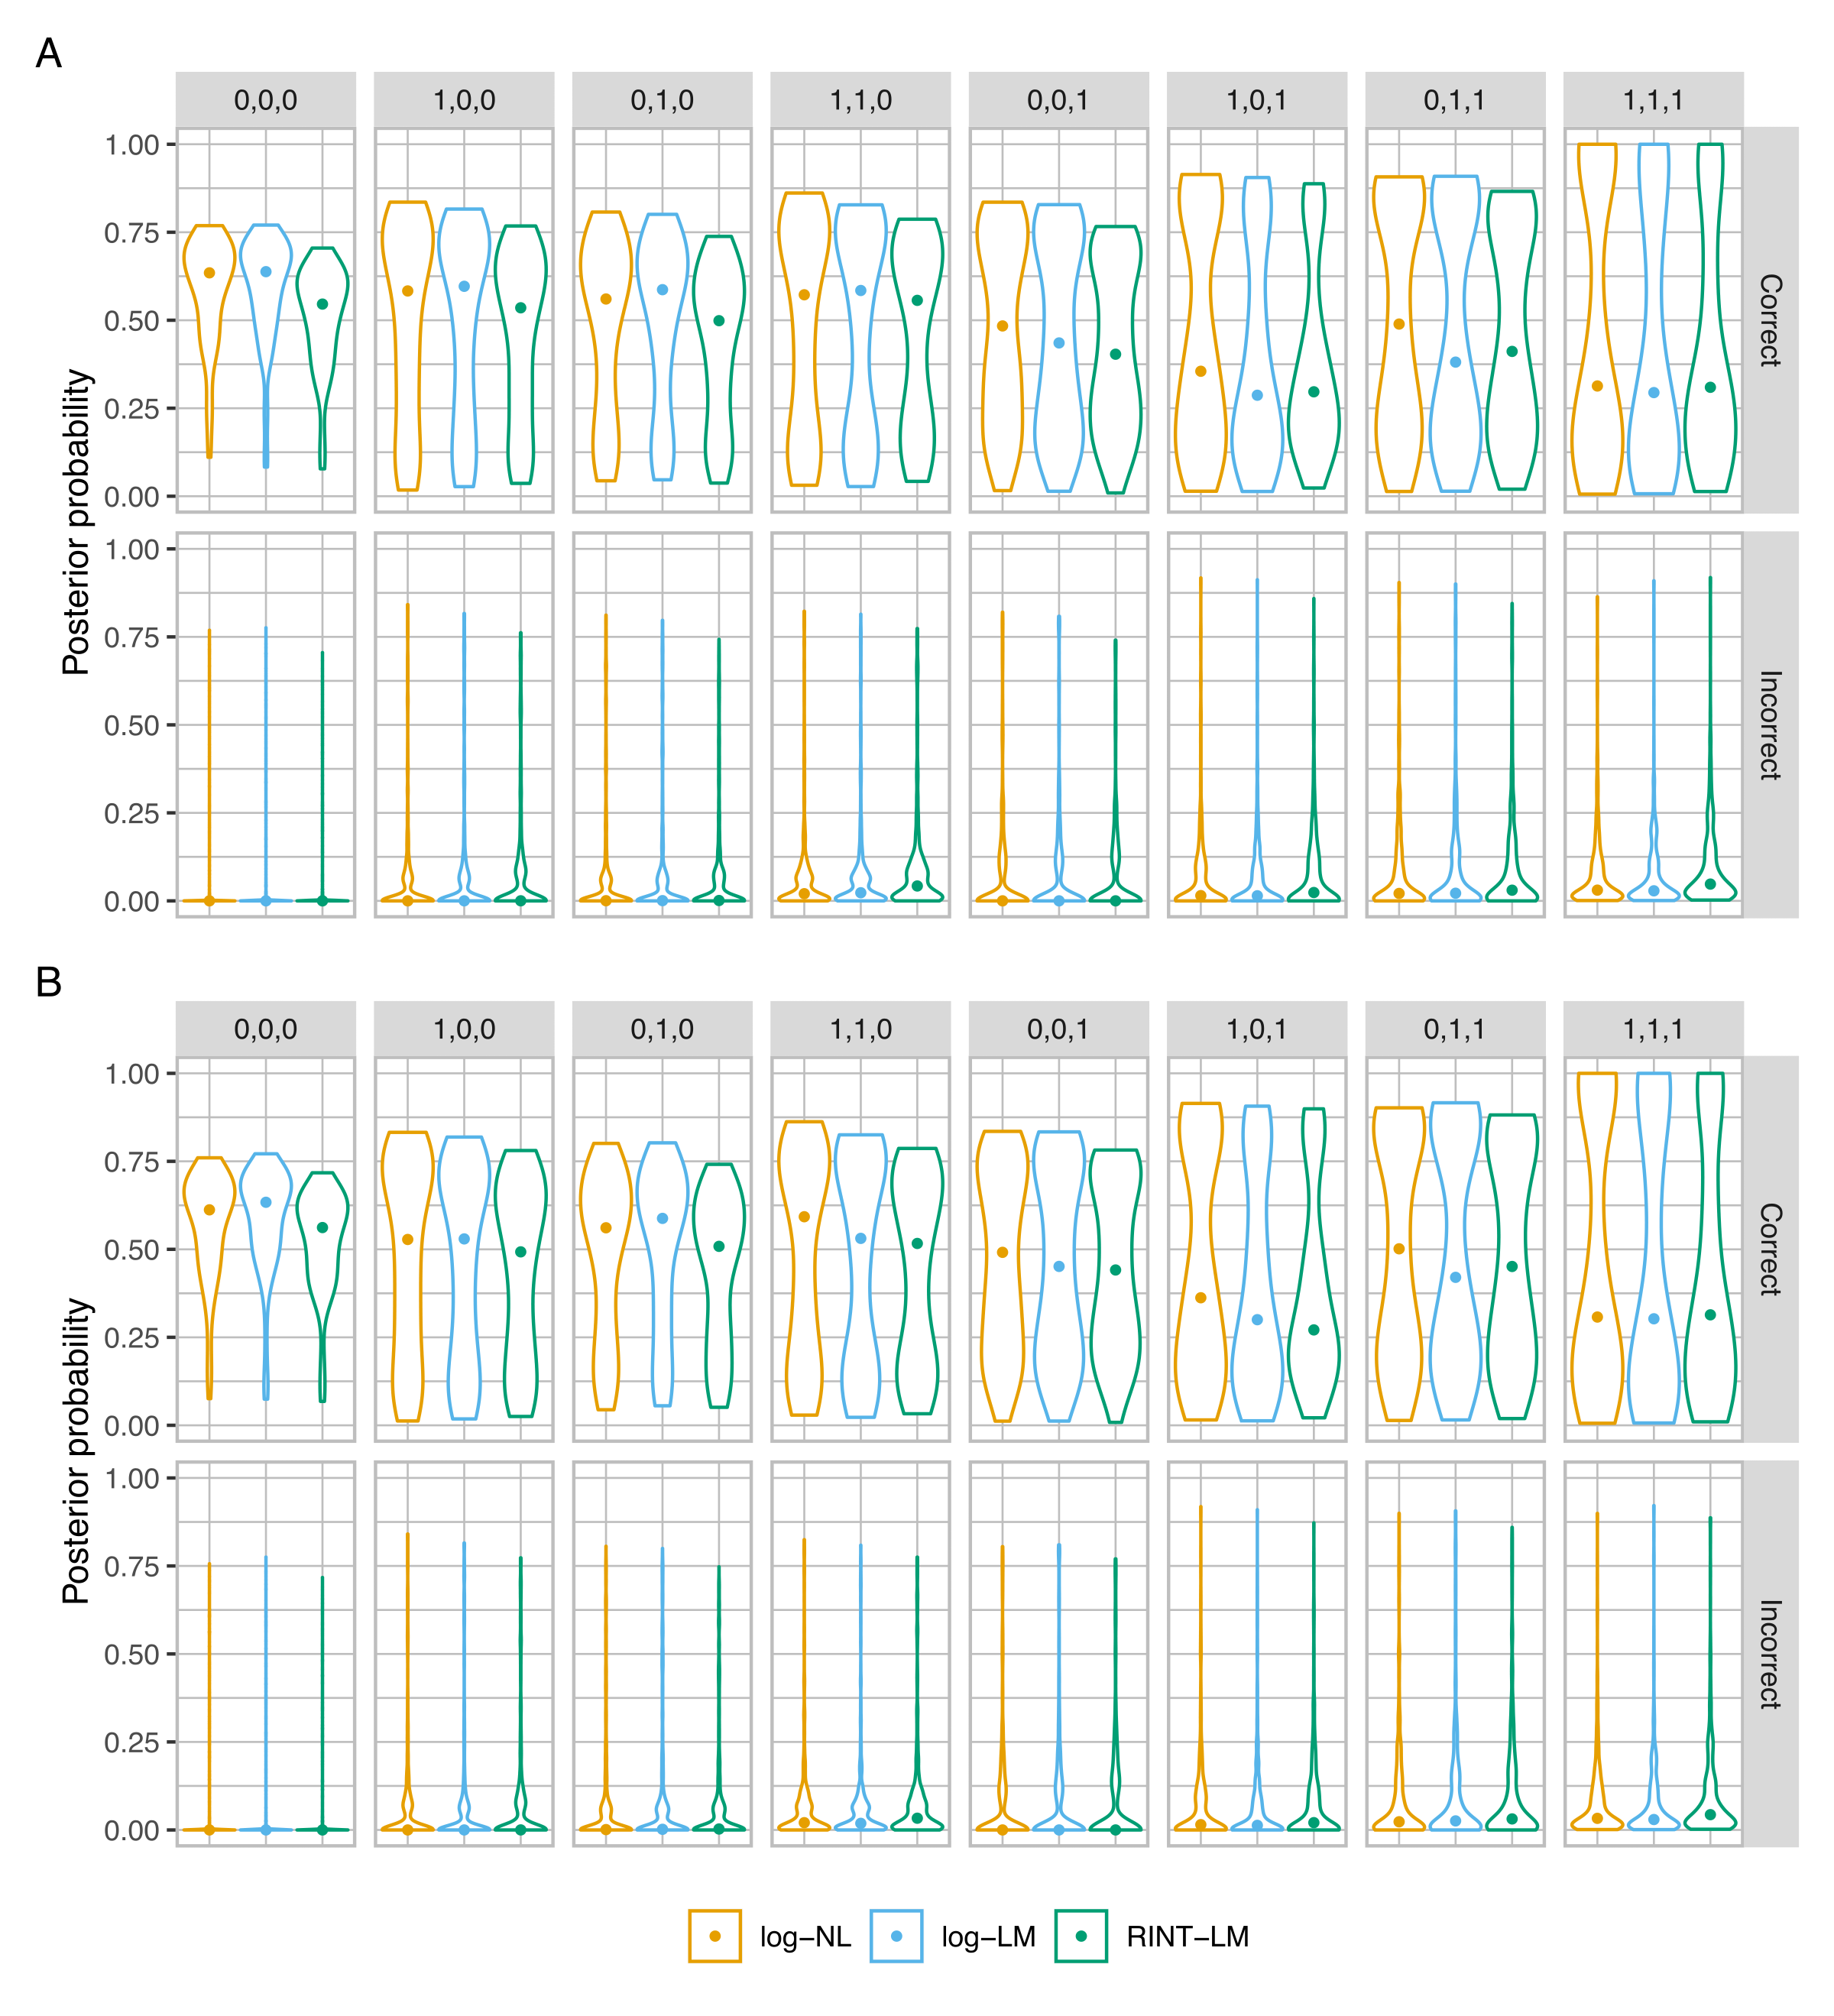
\includegraphics[width=0.8\textwidth]{png/sim_vln_mcmc_bs1.png}
\end{center}  
\caption{
  {\bf
    S7 Fig.
    Posterior probability of the correct and incorrect models for the eight categories obtained by BMS using MCMC and bridge sampling on data generated without random effect.}
Violin plots for comparing the performance of BMS with $\log$-NL, $\log$-LM, and RINT-LM based on the distribution of posterior probability of the correct and incorrect models for each of the eight model categories. The closed circles represent median values. The panels \textbf{A} and \textbf{B} respectively show the results in scenarios 1 and 2, which are described in the legend to \sfigroccmcmc.
}
\label{s-fig:sim-vln-mcmc1}
\end{figure}

\begin{figure}[!ht]
\begin{center}
  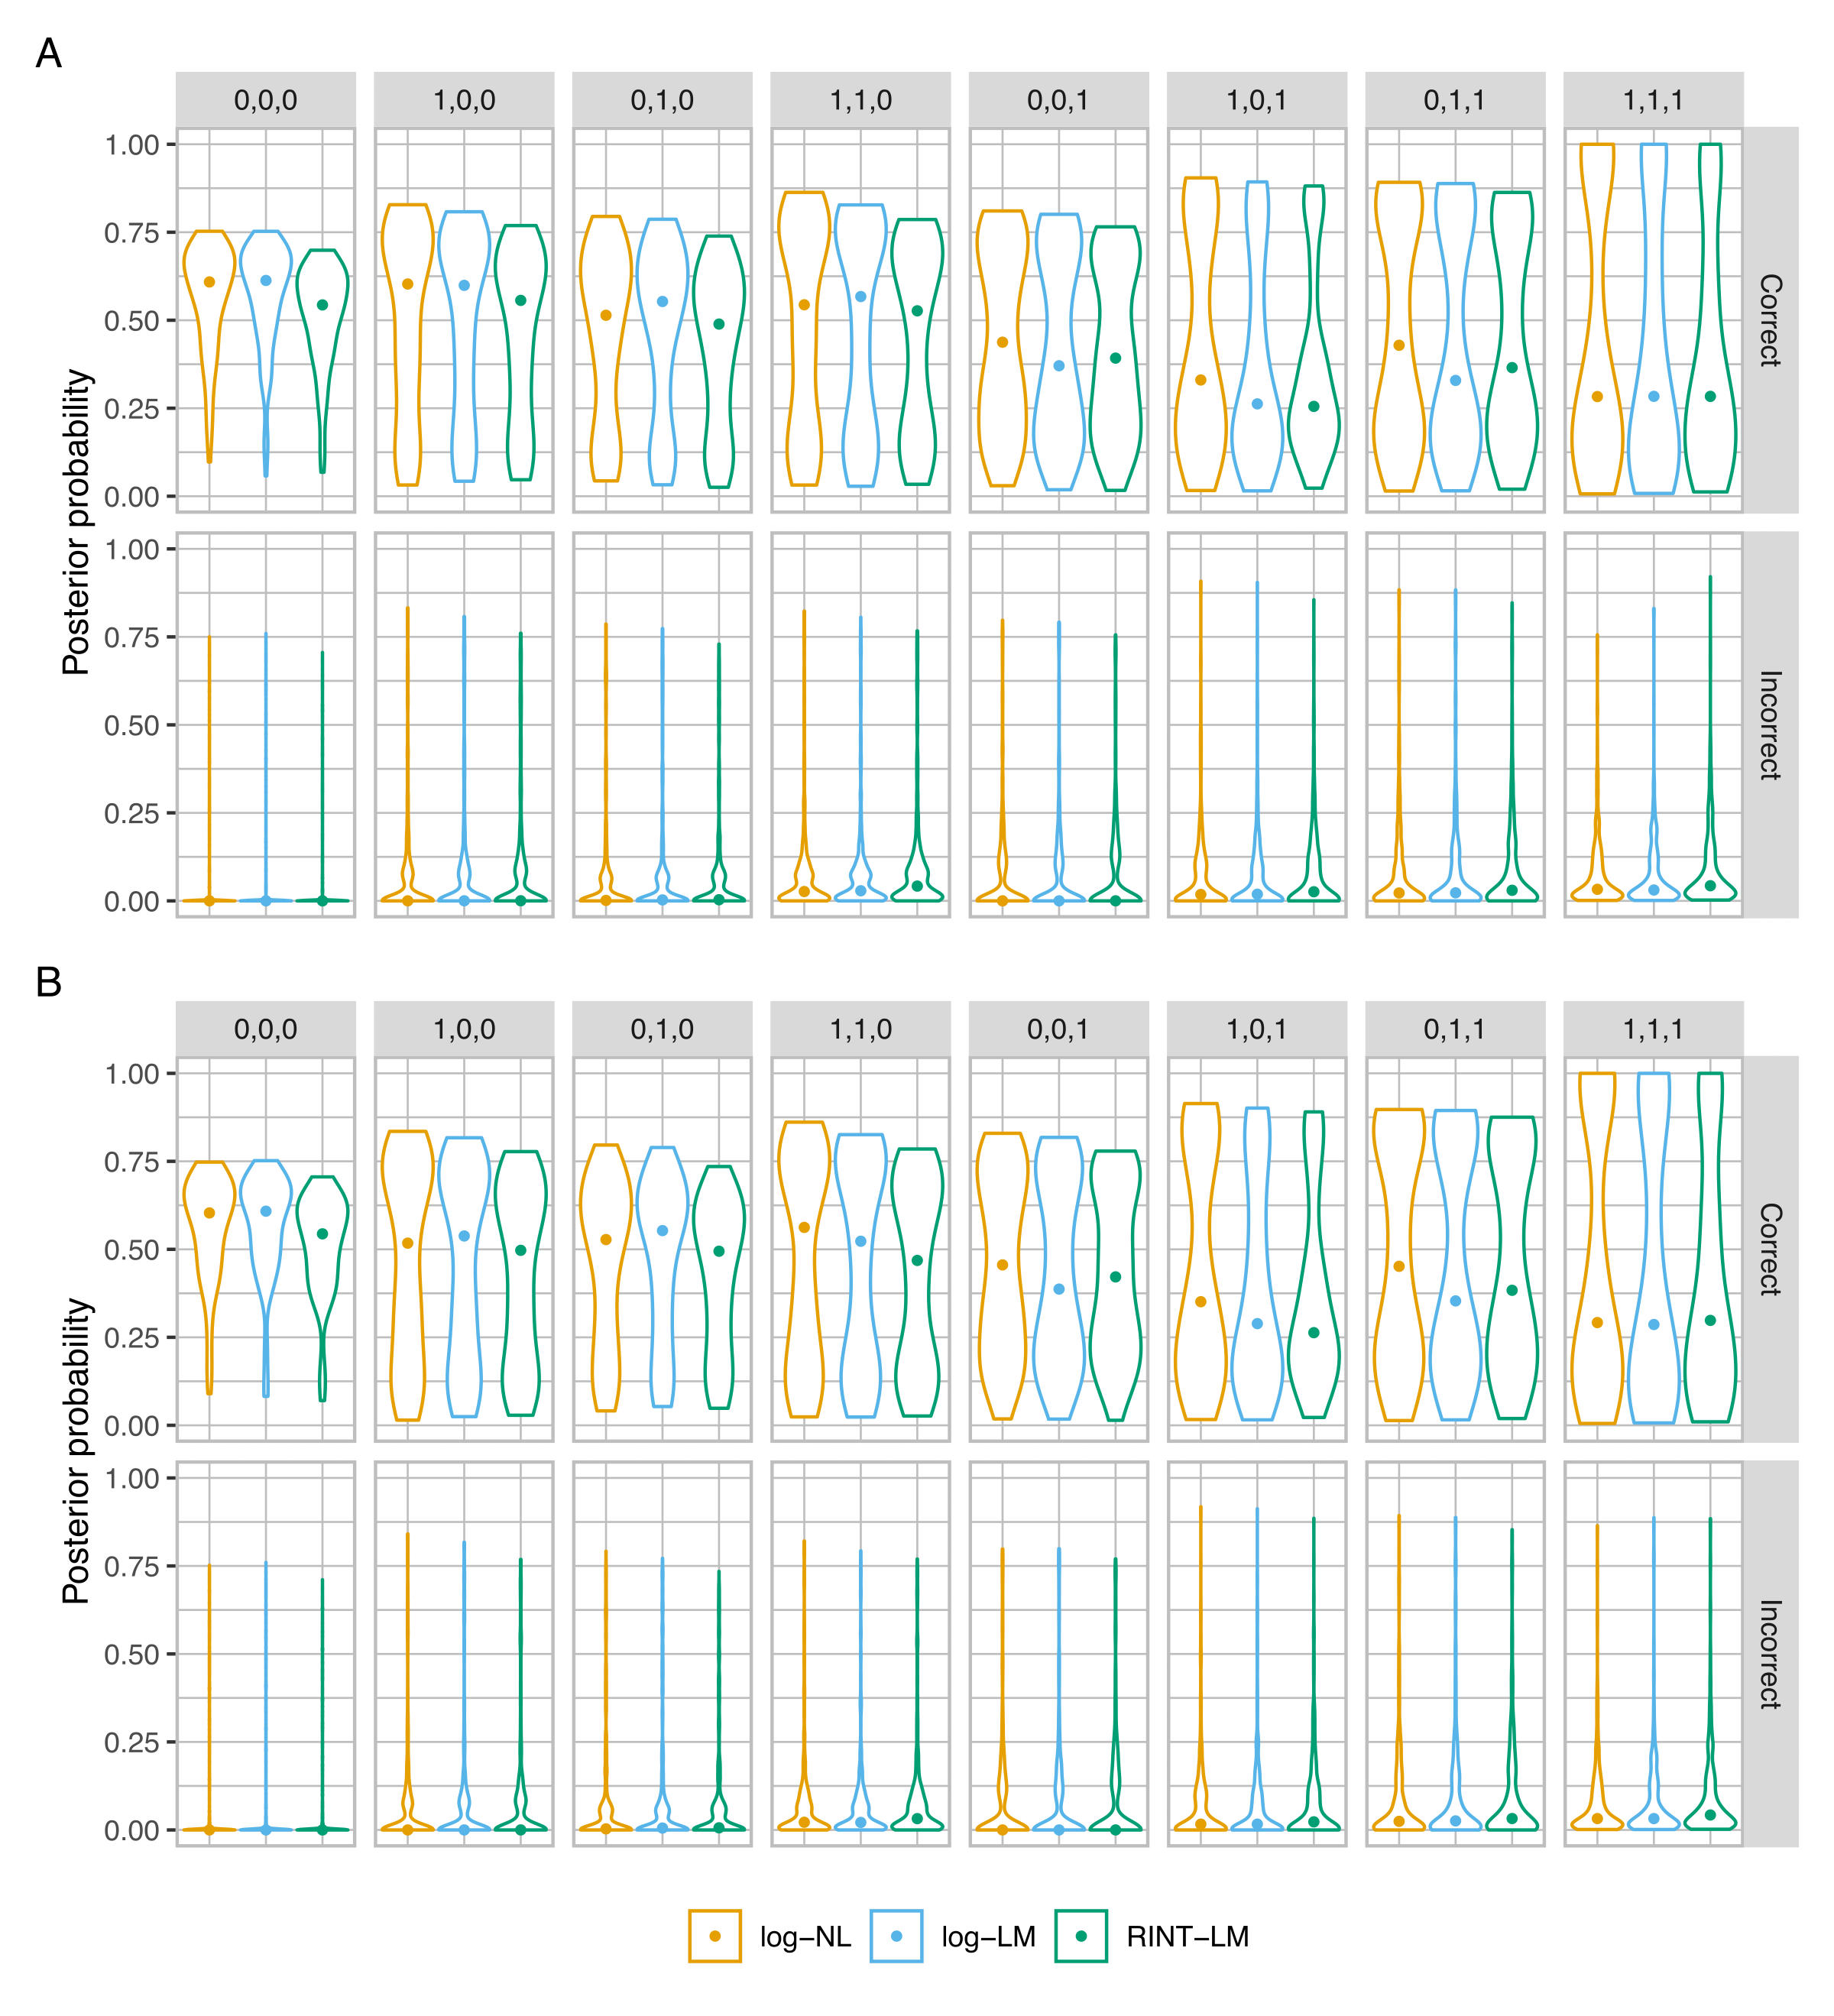
\includegraphics[width=0.8\textwidth]{png/sim_vln_mcmc_bs2.png}
\end{center}  
\caption{
  {\bf
    S7.2 Fig.
    Posterior probability of the correct and incorrect models for the eight categories obtained by BMS using MCMC and bridge sampling on data generated with donor random effect.}
The same as \sfigppmcmcone but on data generated with donor random effect. The panels \textbf{A} and \textbf{B} respectively show the results in scenarios 3 and 4, which are described in the legend to \sfigroccmcmc.
}
\label{s-fig:sim-vln-mcmc2}
\end{figure}

\begin{figure}[!ht]
\begin{center}
  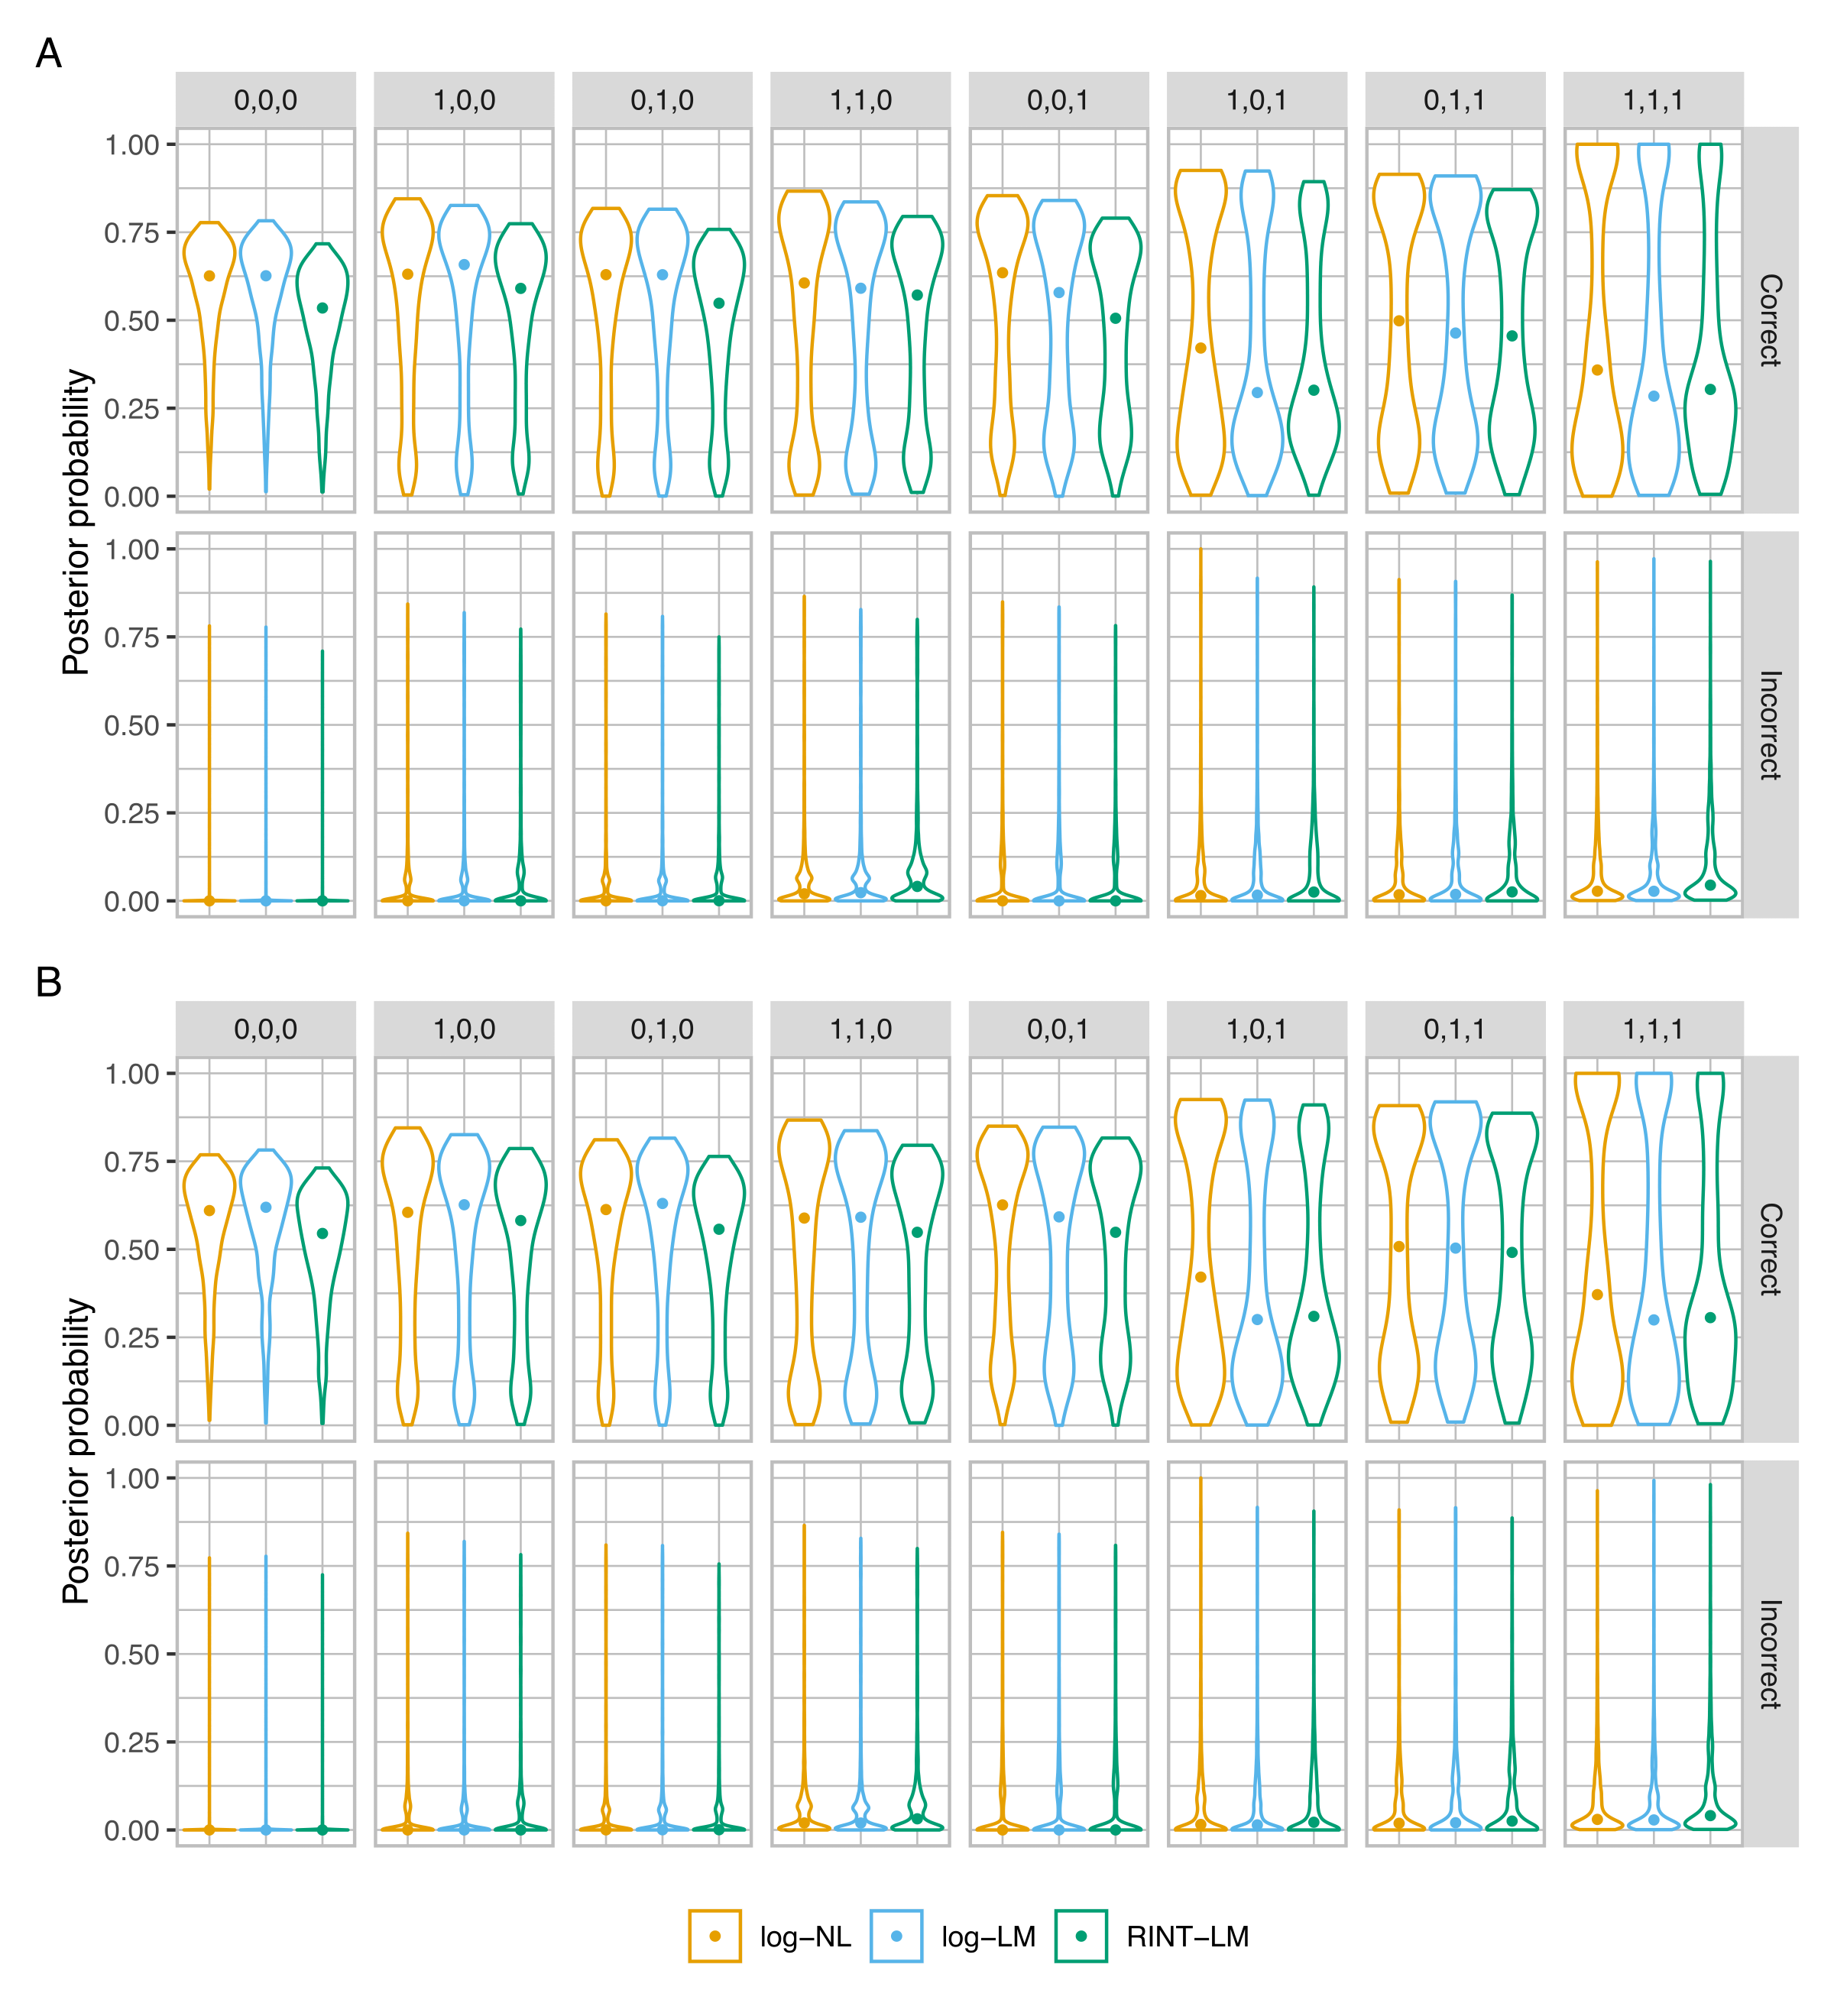
\includegraphics[width=0.8\textwidth]{png/sim_vln_map_lap1.png}
\end{center}  
\caption{
  {\bf
    S7.3 Fig.
    Posterior probability of the correct and incorrect models for the eight categories obtained by BMS using MAP estimation and Laplace approximation on data generated without random effect.}
The same as in \sfigppmcmcone but for MAP estimation and Laplace approximation.
}
\label{s-fig:sim-vln-map1}
\end{figure}

\begin{figure}[!ht]
\begin{center}
  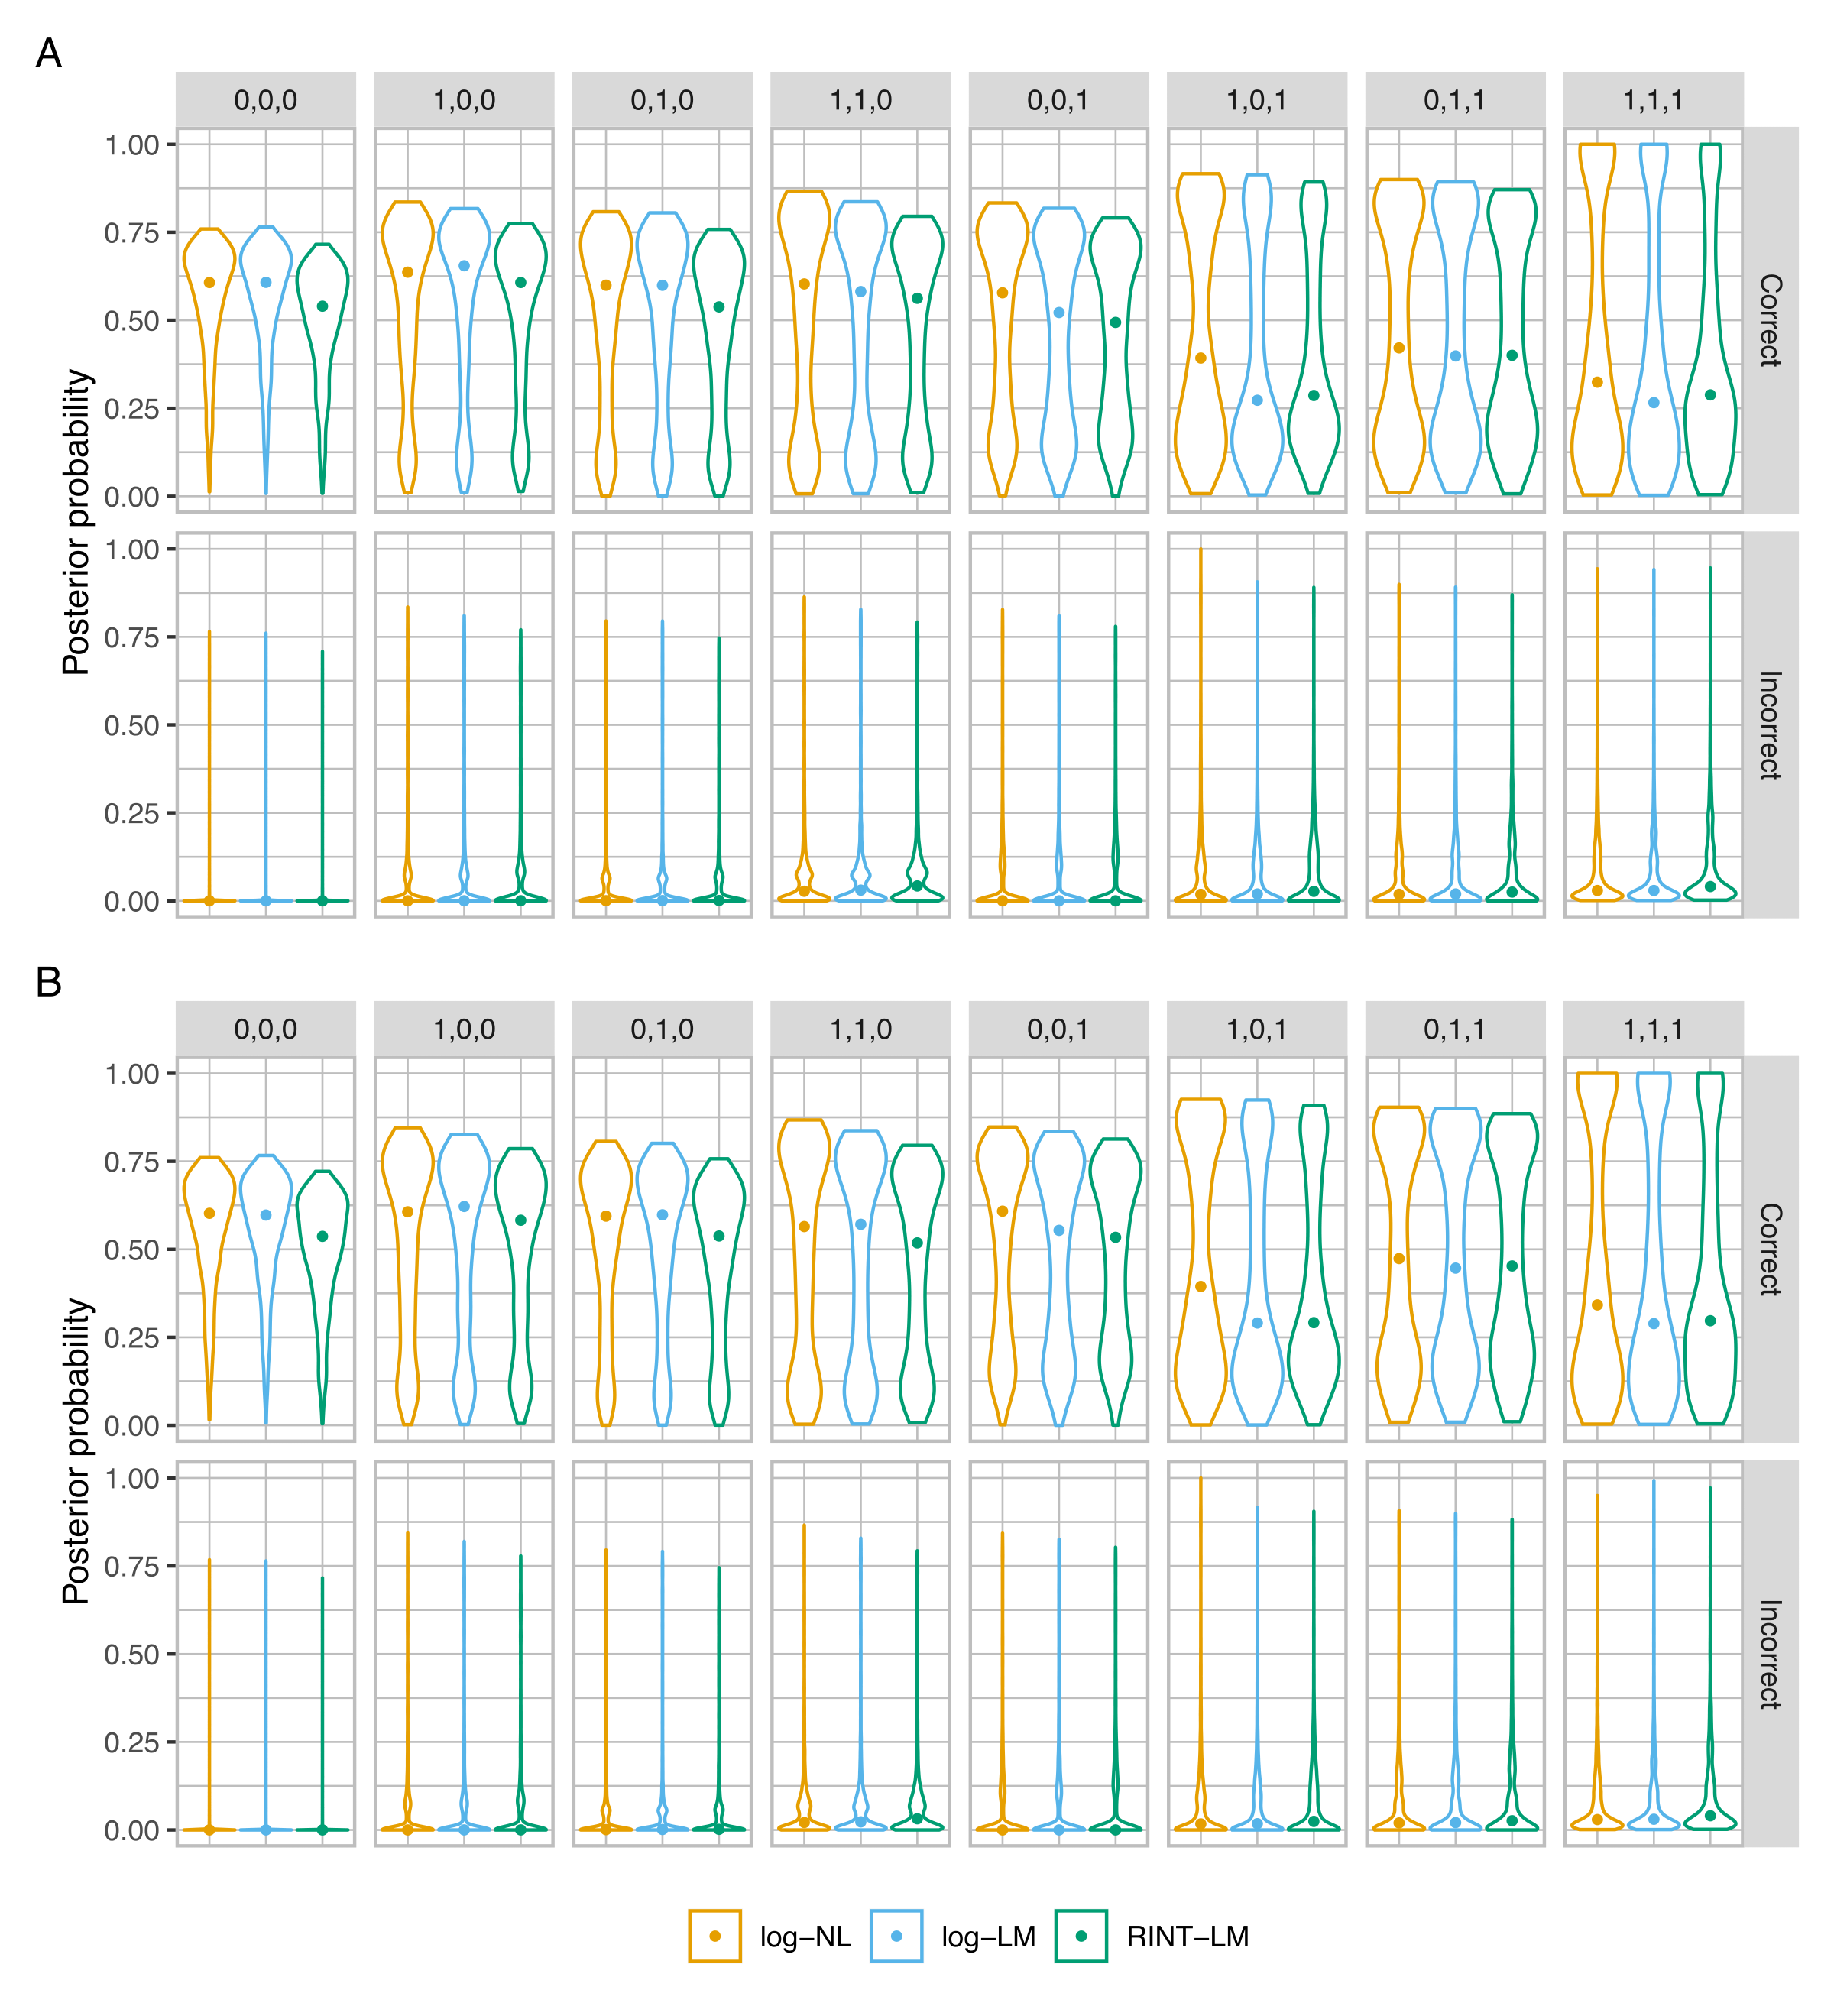
\includegraphics[width=0.8\textwidth]{png/sim_vln_map_lap2.png}
\end{center}  
\caption{
  {\bf
    S7.4 Fig.
    Posterior probability of the correct and incorrect models for the eight categories obtained by BMS using MAP estimation and Laplace approximation on data generated with donor random effect.}
The same as in \sfigppmcmctwo but for MAP estimation and Laplace approximation.
}
\label{s-fig:sim-vln-map2}
\end{figure}

\begin{figure}[!ht]
\begin{center}
  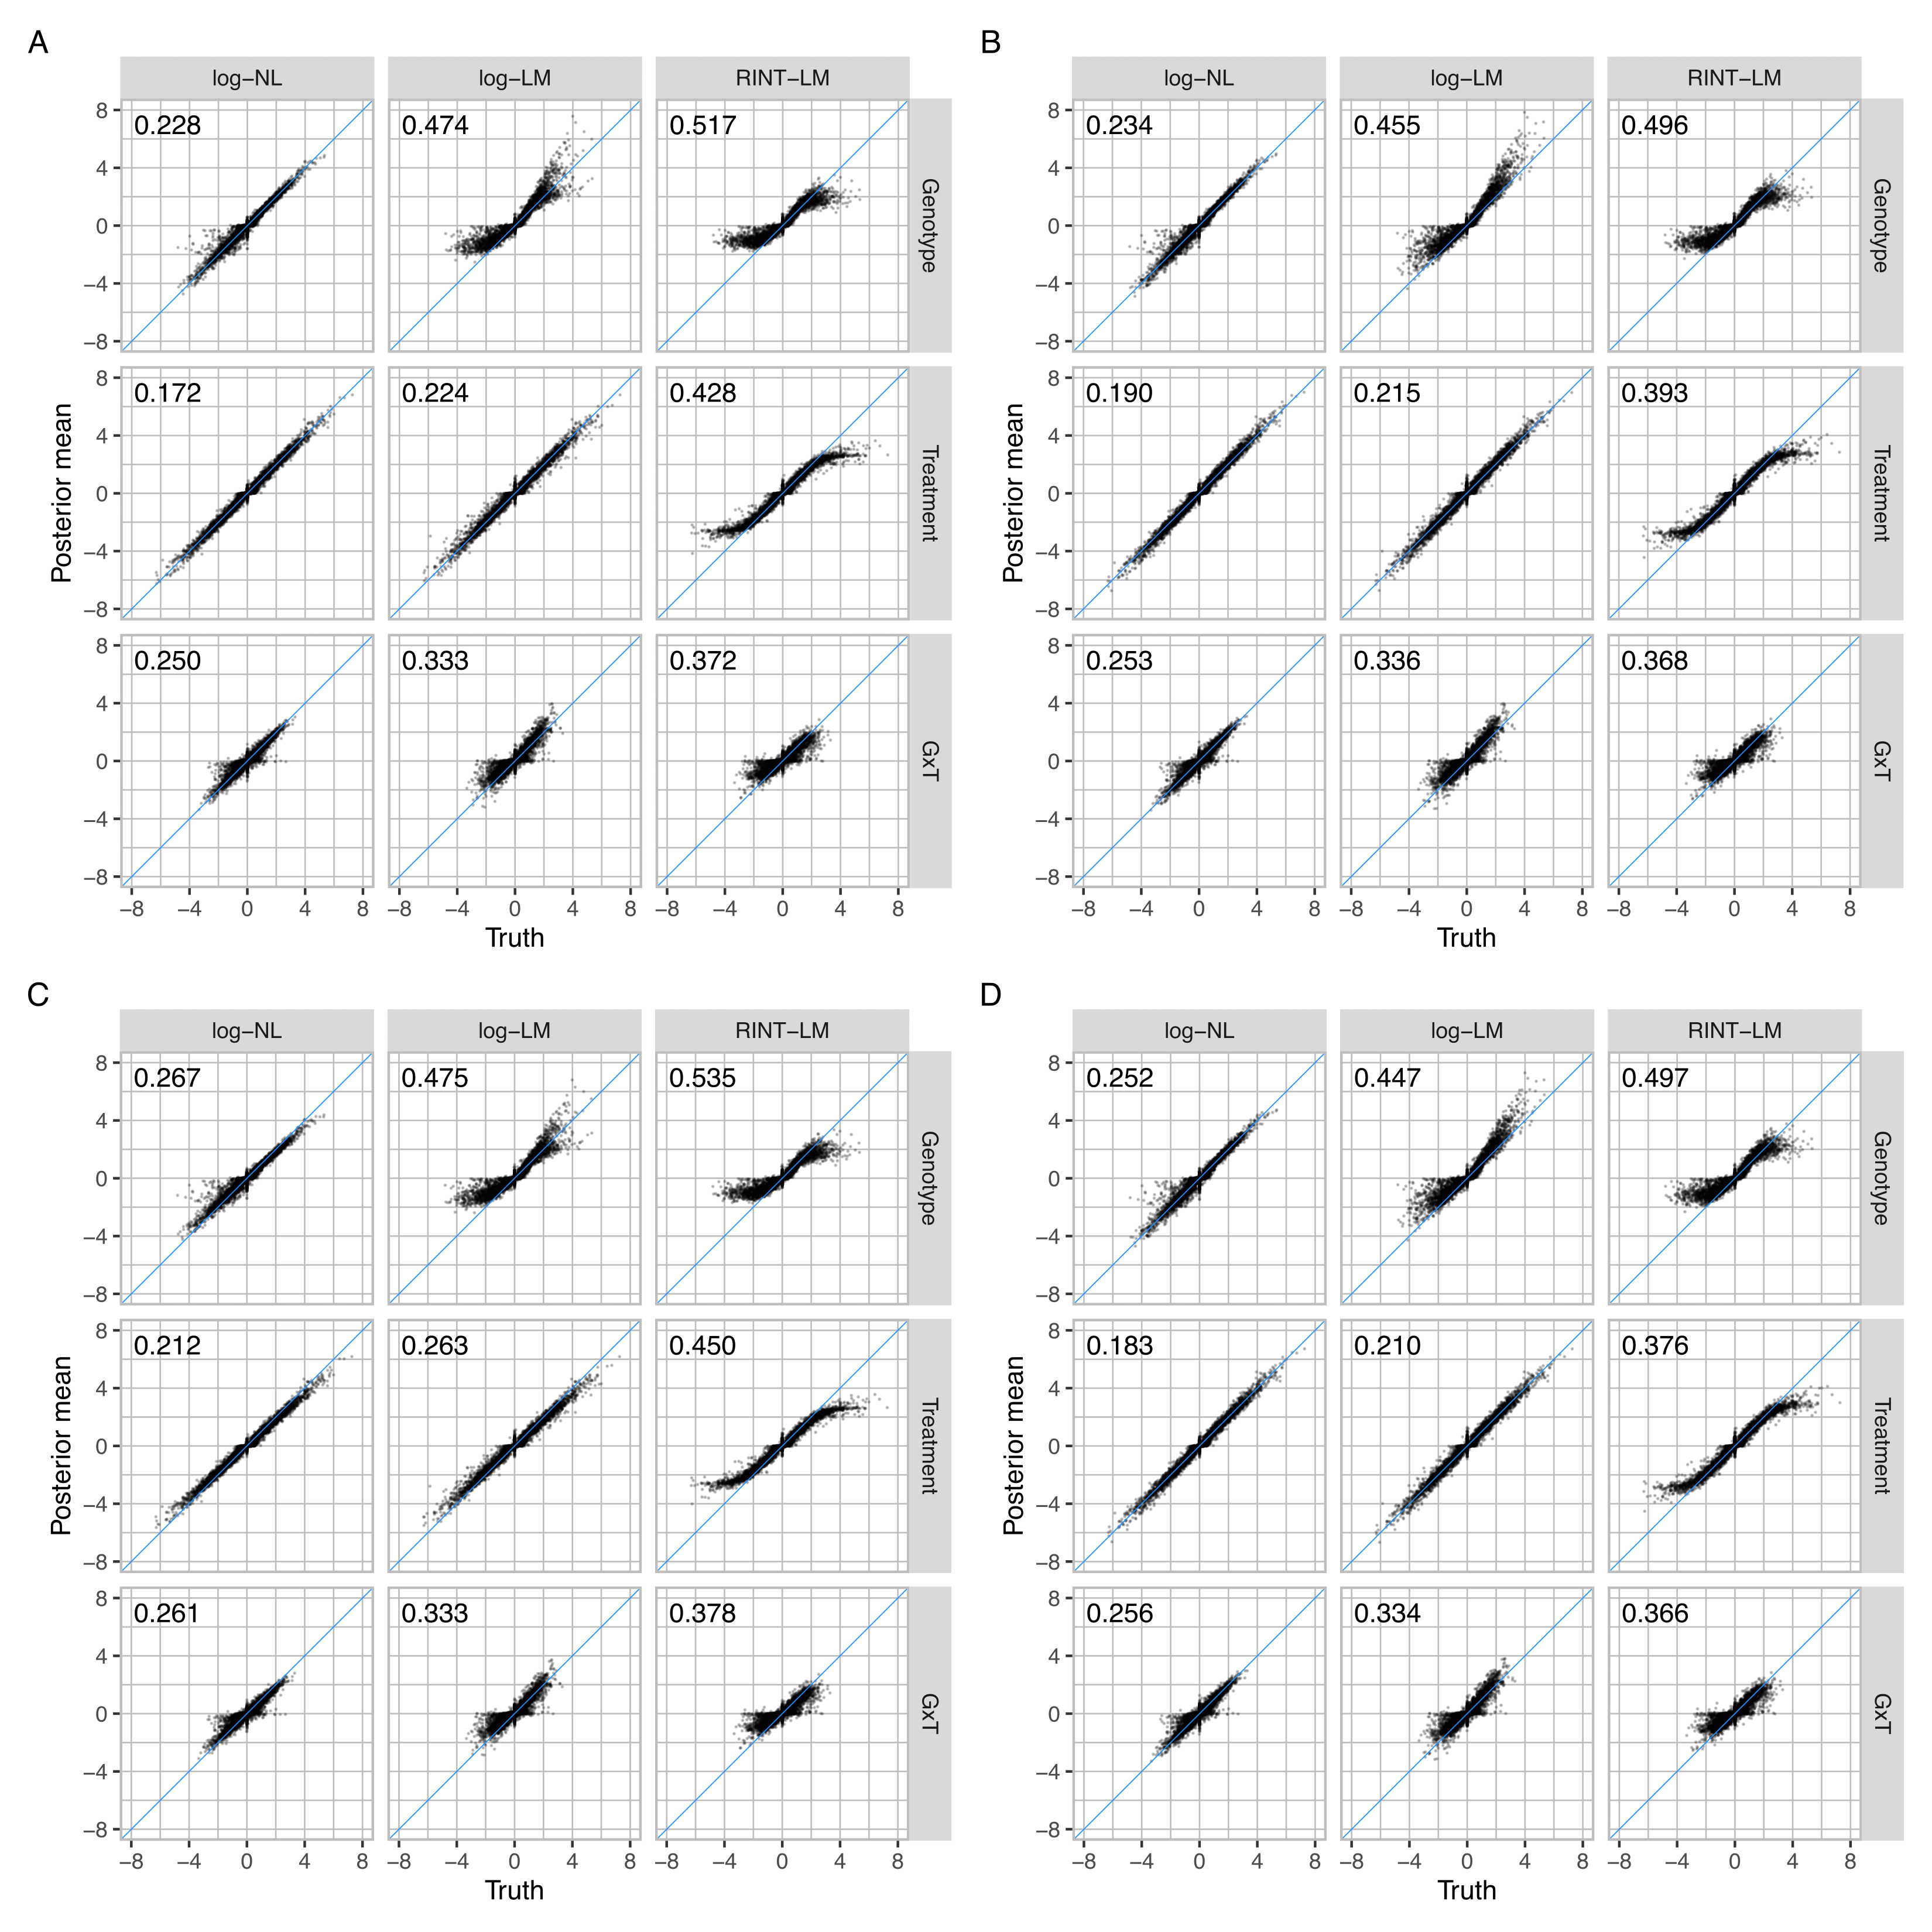
\includegraphics[width=1\textwidth]{png/sim_est_mcmc_bs.png}
\end{center}  
\caption{
  {\bf
    S8 Fig.
    Comparison of effect estimates by Bayesian model averaging with $\log$-NL, $\log$-LM, and RINT-LM.}
\textbf{A.} Scatter plots comparing estimation of the genotype, treatment, and \GxT interaction effects relative to the residual standard deviation against the true values in scenario 1, which is described in the legend to \sfigroccmcmc.
Each point represents each of 8000 feature-SNP pairs.
Shown in the top-left corner of each panel is the root mean squared error (RMSE).
\textbf{B.} The same as in \textbf{A} but for scenario 2.
\textbf{C.} The same as in \textbf{A} but for scenario 3.
\textbf{D.} The same as in \textbf{A} but for scenario 4.
}
\label{s-fig:sim-est-mcmc-bs}
\end{figure}

\begin{figure}[!ht]
\begin{center}
  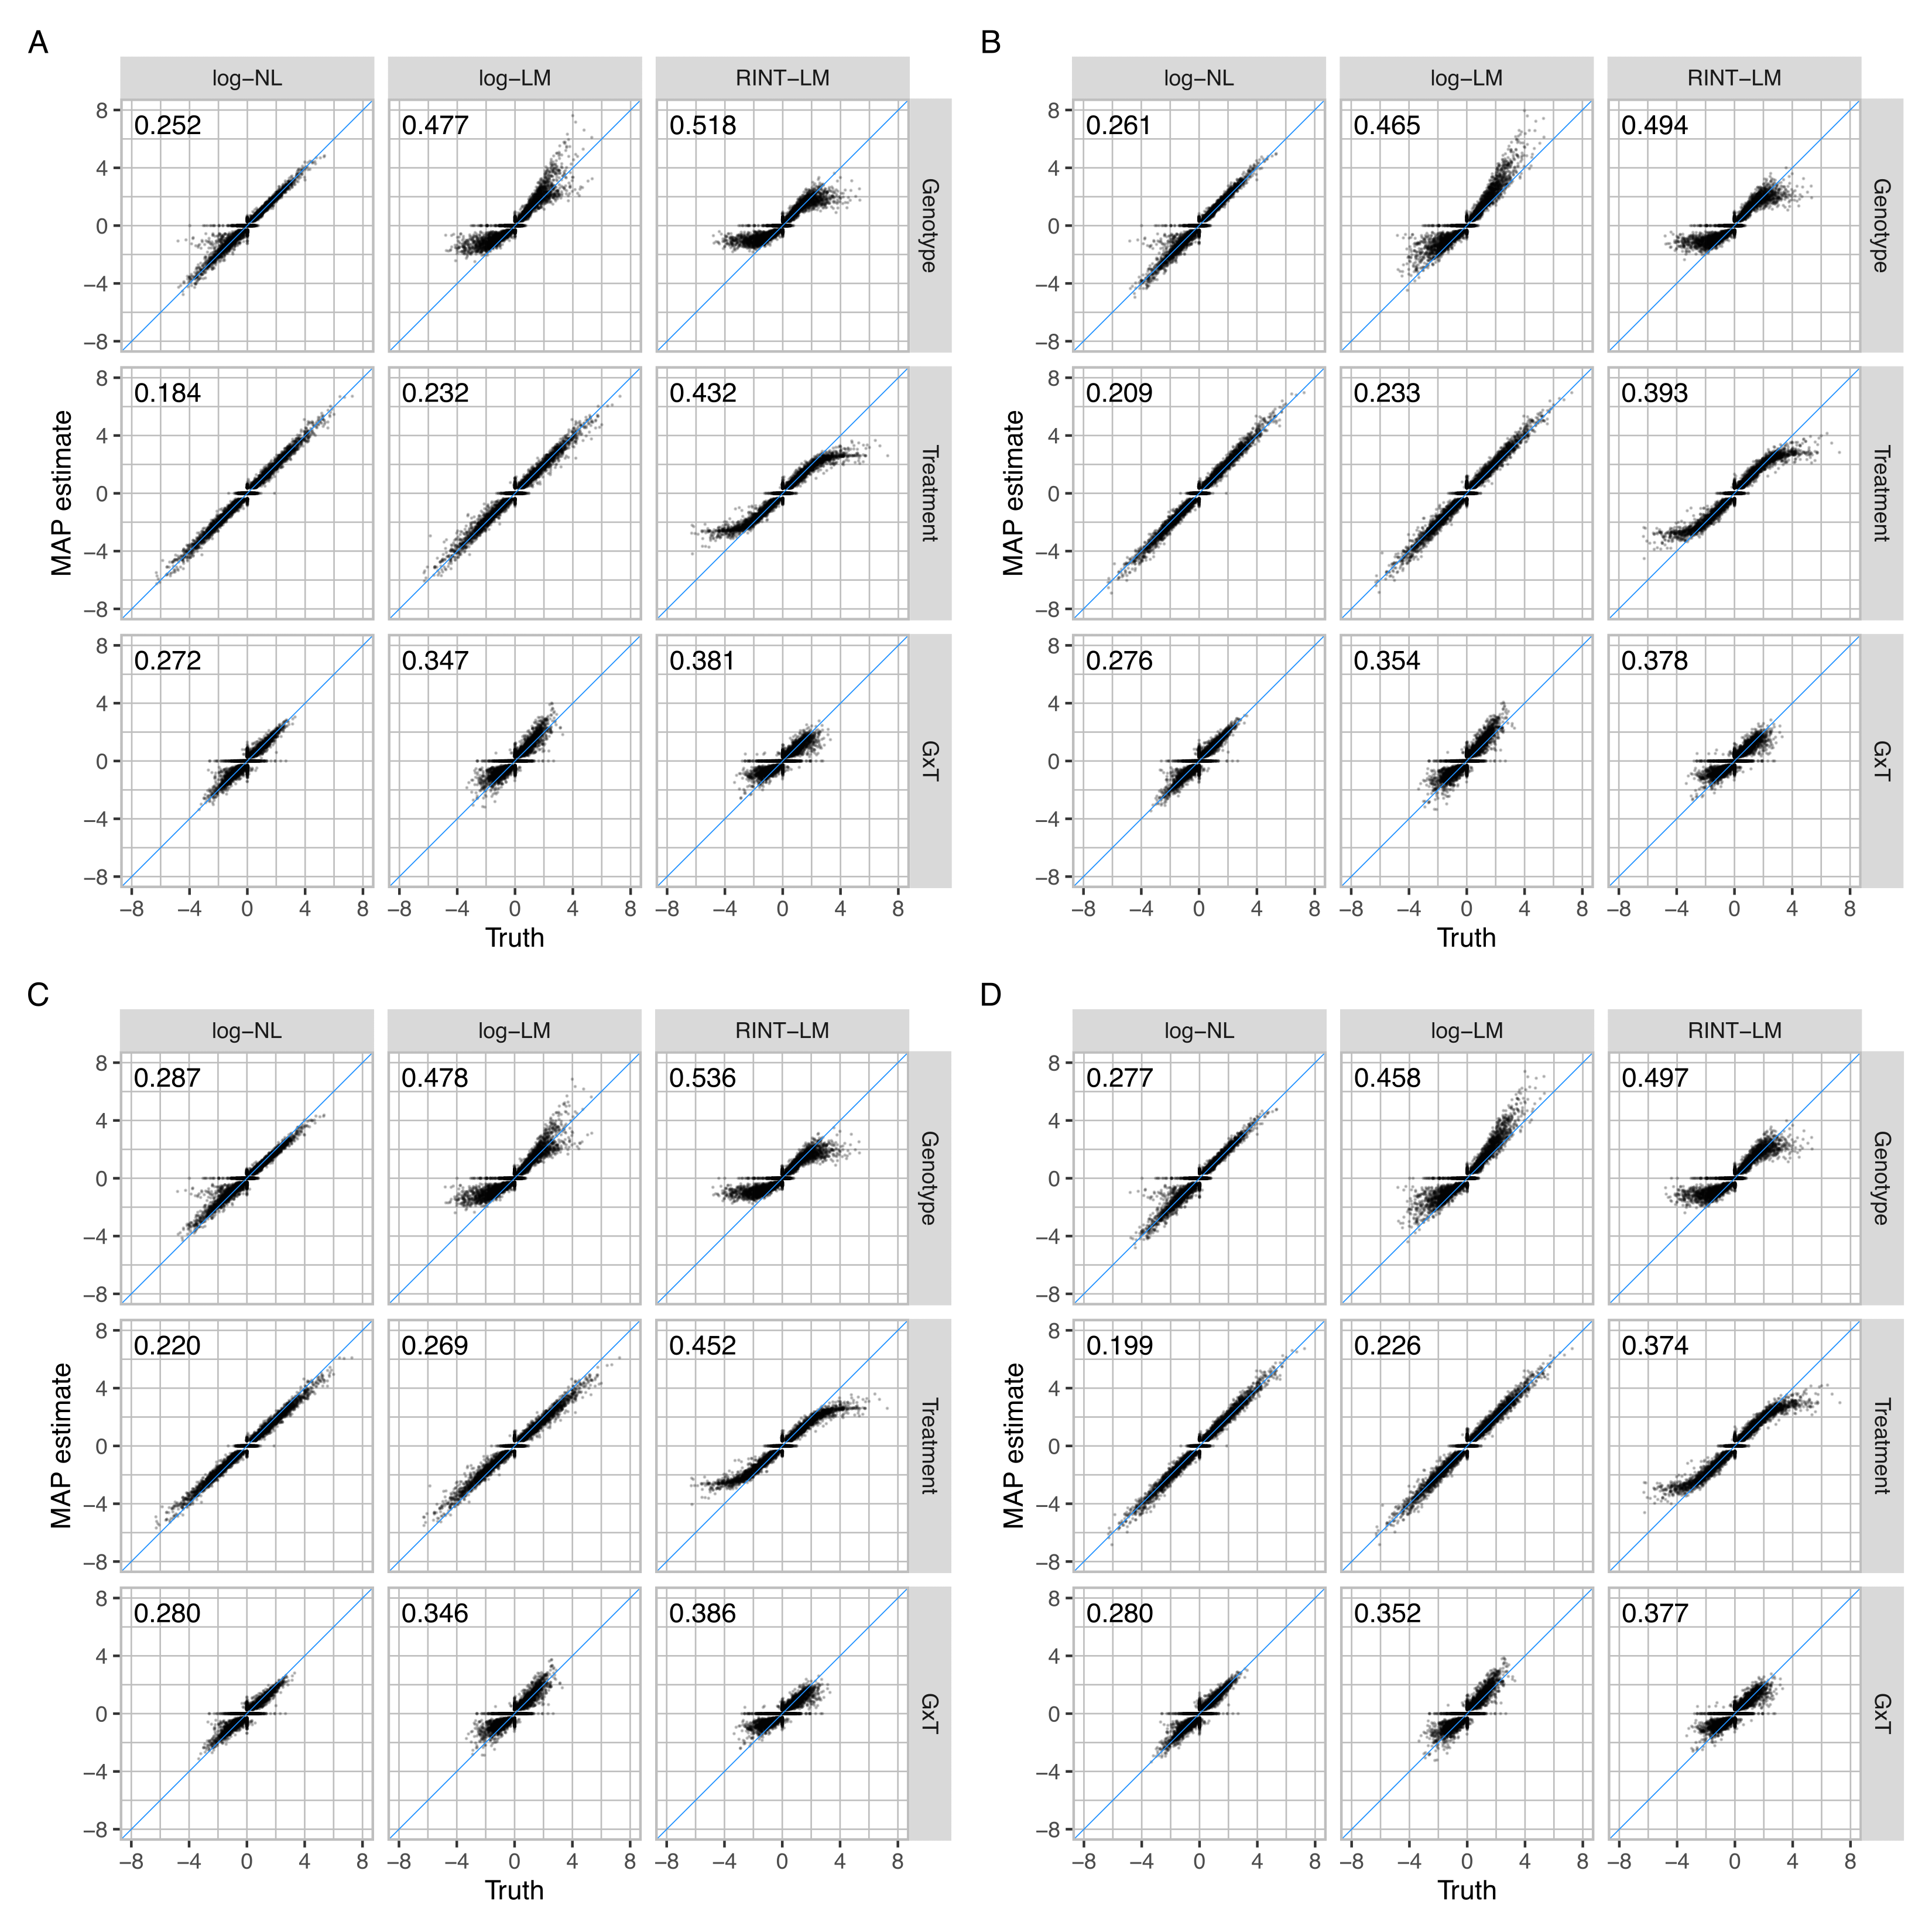
\includegraphics[width=1\textwidth]{png/sim_est_map_lap.png}
\end{center}  
\caption{
  {\bf
    S8.2 Fig.
    Comparison of MAP estimates with $\log$-NL, $\log$-LM, and RINT-LM.}
The same as in \sfigestmcmc but for MAP estimation.
}
\label{s-fig:sim-est-map-lap}
\end{figure}

\begin{figure}[!ht]
\begin{center}
  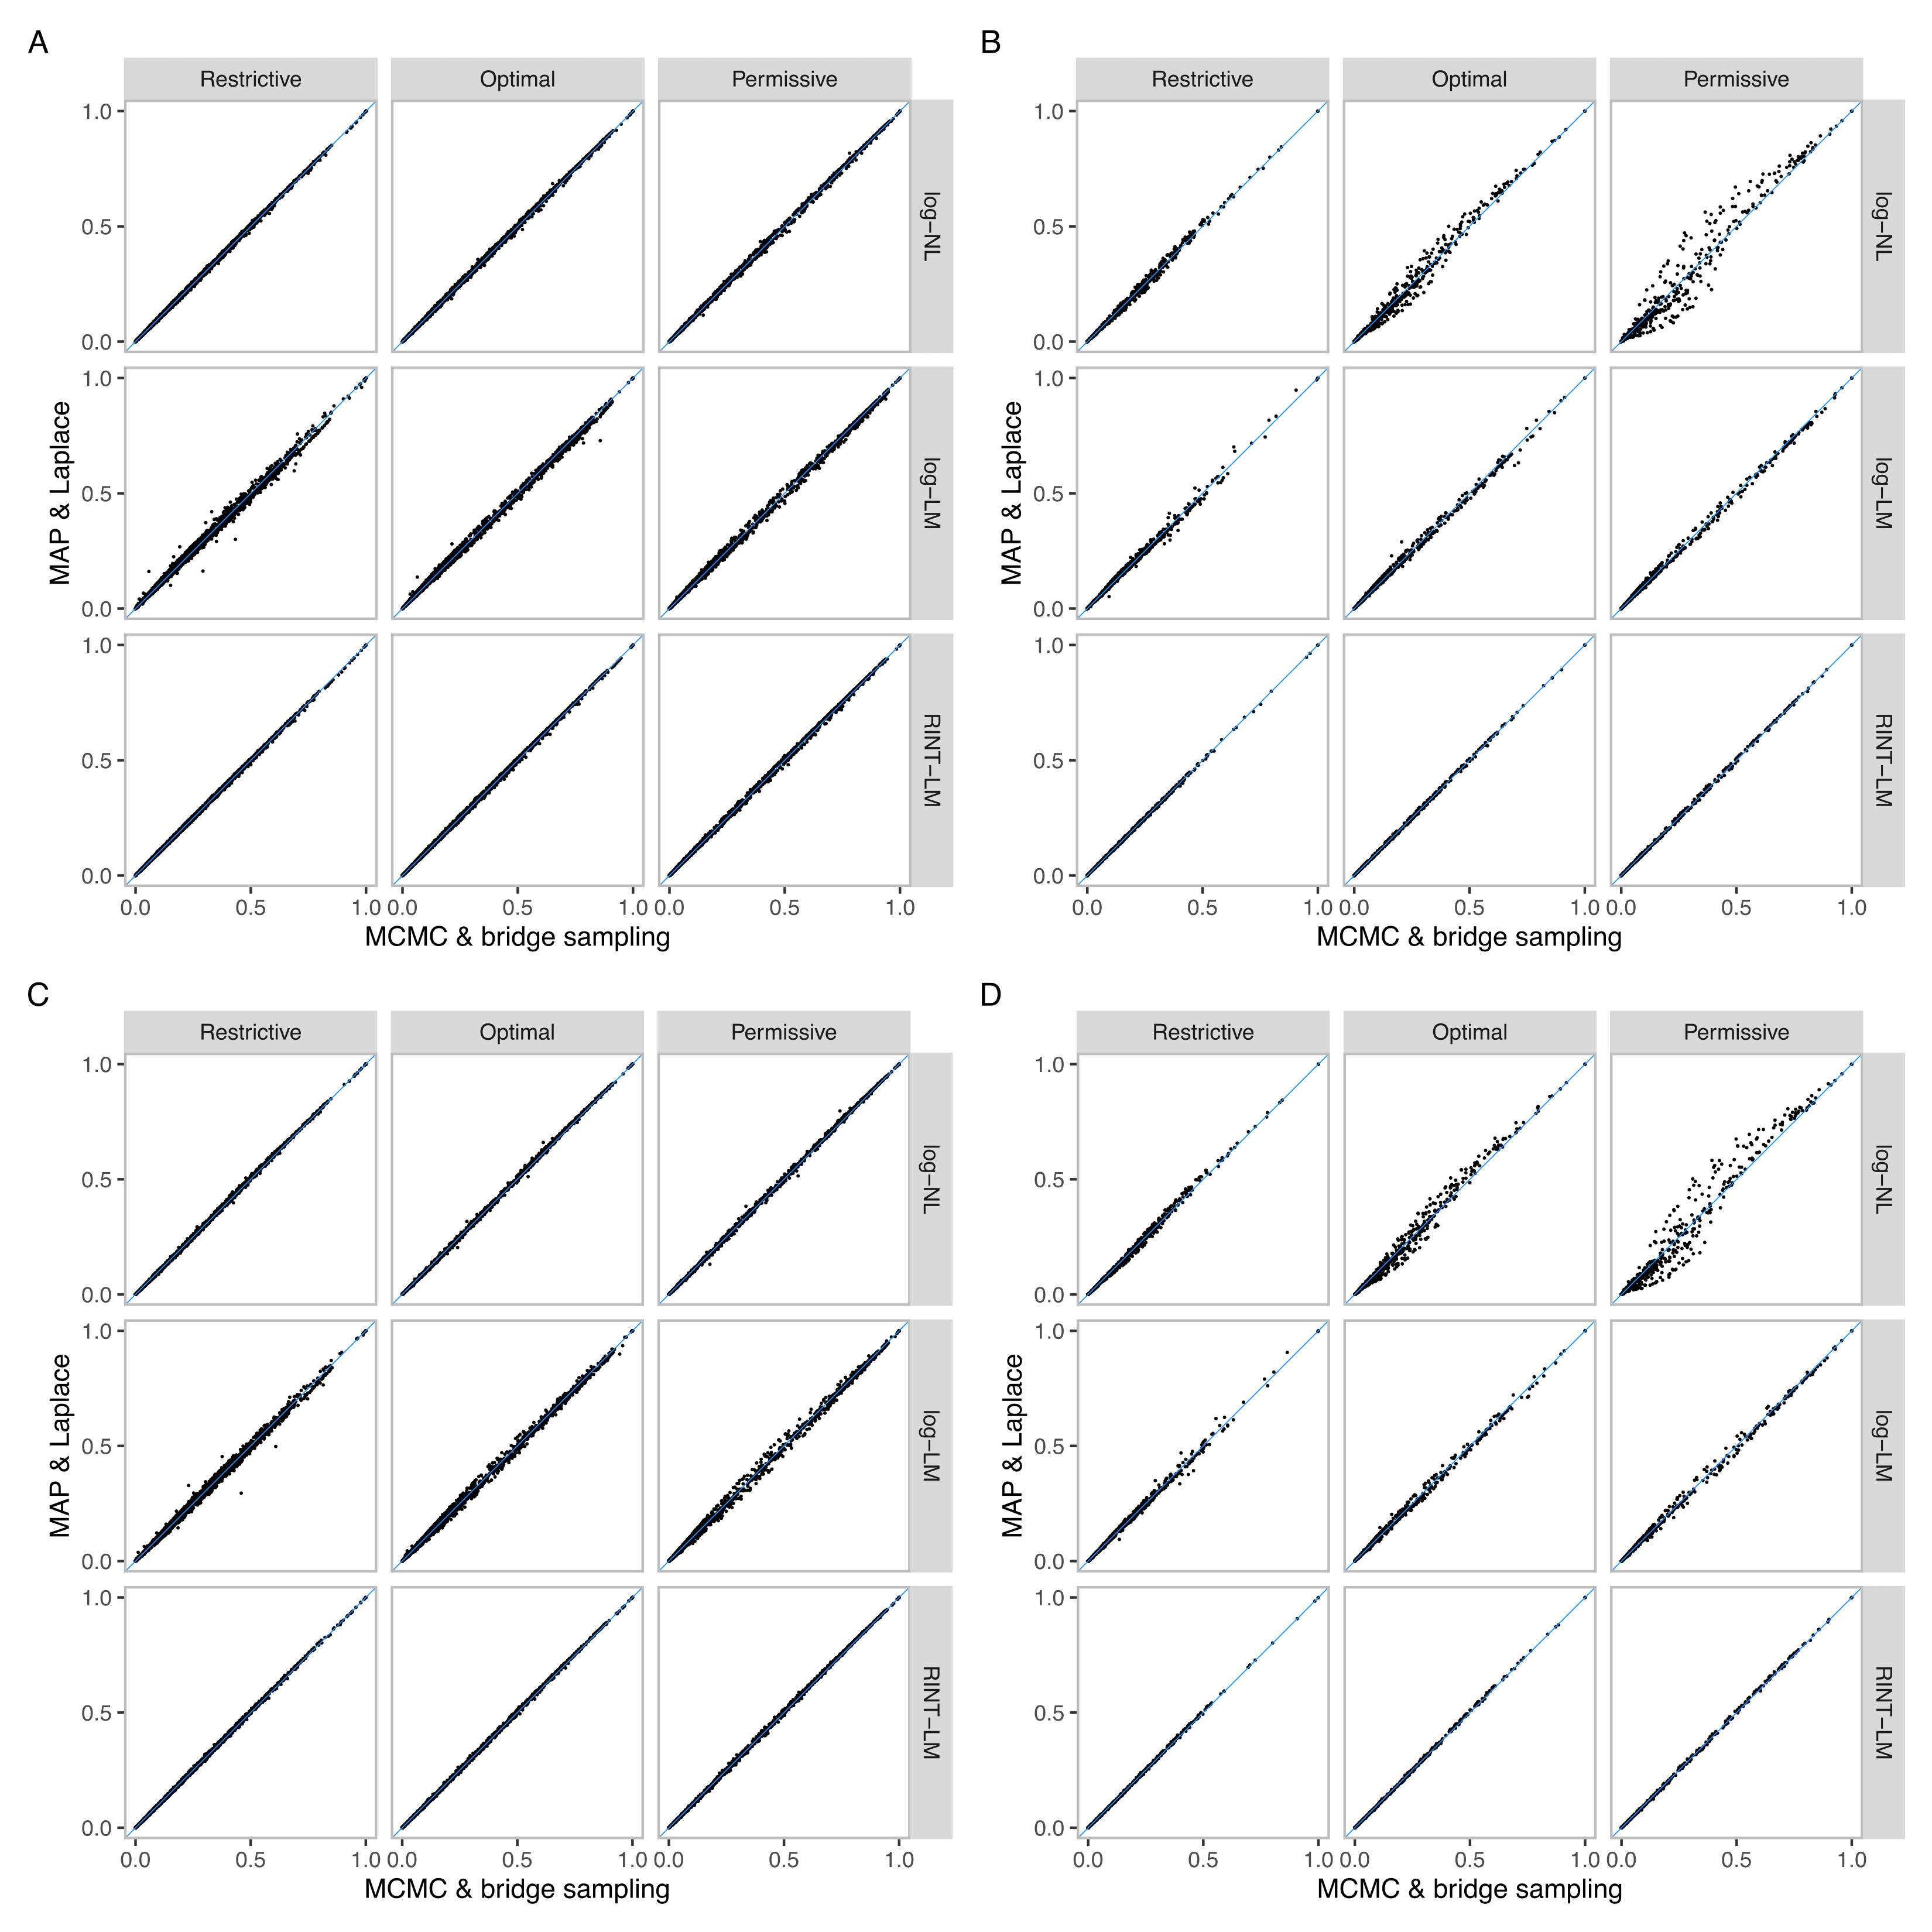
\includegraphics[width=1\textwidth]{png/sim_compare_pp_noranef.png}
\end{center}  
\caption{
  {\bf
    S9 Fig.
    Comparison of posterior probability at varying hyperparameter values between two computational approaches on synthetic data generated without donor random effect.}
\textbf{A.} Scatter plots comparing posterior probabilities obtained by MCMC followed by bridge sampling and those obtained by MAP estimation followed by Laplace approximation for scenario 1, which is described in the legend to \sfigroccmcmc. Each point represents each of the eight models for a feature-SNP pair. The values are compared across eight models and 686 feature-SNP pairs for which minor allele homozygotes were present (i.e., 5488 combinations).
\textbf{B.} The same as in \textbf{A} but for 114 feature-SNP pairs for which minor allele homozygotes were absent (i.e., 912 combinations).
\textbf{C.} The same as in \textbf{A} but for scenario 2.
\textbf{D.} The same as in \textbf{B} but for scenario 2.
}
\label{s-fig:sim-compare-pp-noranef}
\end{figure}

\begin{figure}[!ht]
\begin{center}
  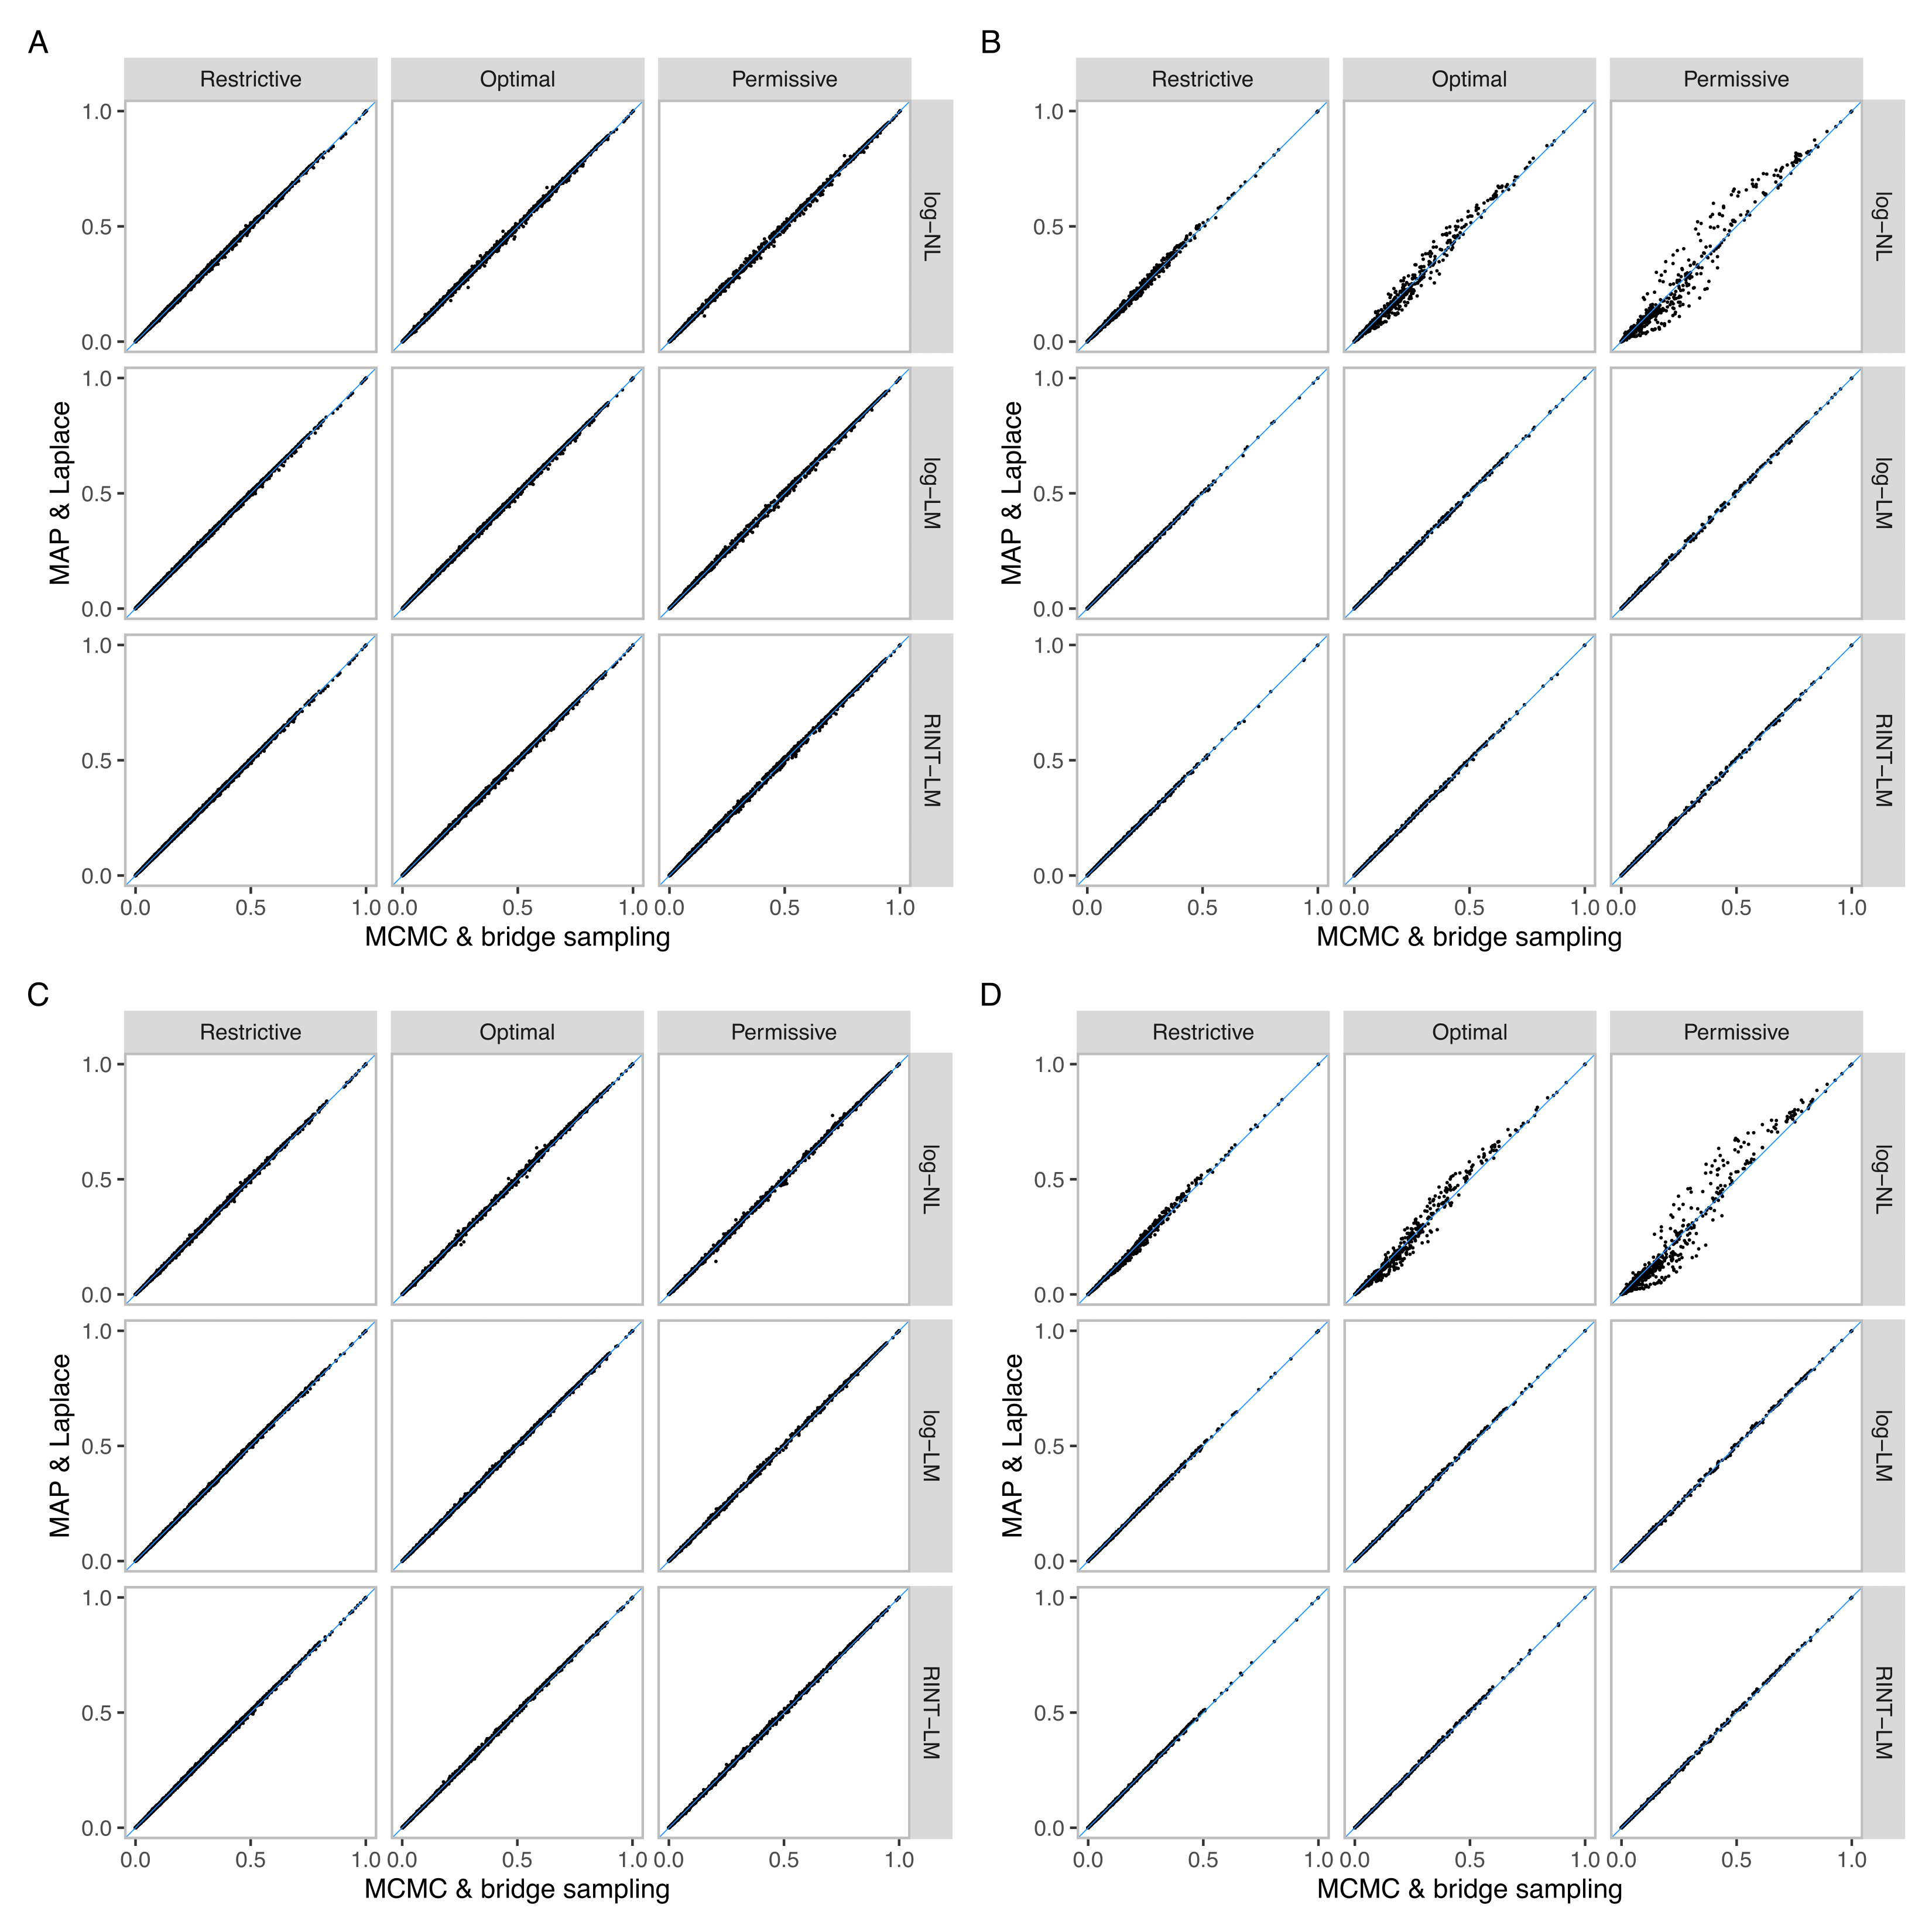
\includegraphics[width=1\textwidth]{png/sim_compare_pp_ranef.png}
\end{center}  
\caption{
  {\bf
    S9.2 Fig.
    Comparison of posterior probability at varying hyperparameter values between two computational approaches on synthetic data generated with donor random effect.}
\textbf{A.} The same as in \sfigcompnoranef \textbf{A} but for scenario 2.
\textbf{B.} The same as in \sfigcompnoranef \textbf{B} but for scenario 2.
\textbf{C.} The same as in \sfigcompnoranef \textbf{C} but for scenario 3.
\textbf{D.} The same as in \sfigcompnoranef \textbf{D} but for scenario 3.
}
\label{s-fig:sim-compare-pp-ranef}
\end{figure}

\begin{figure}[!ht]
\begin{center}
  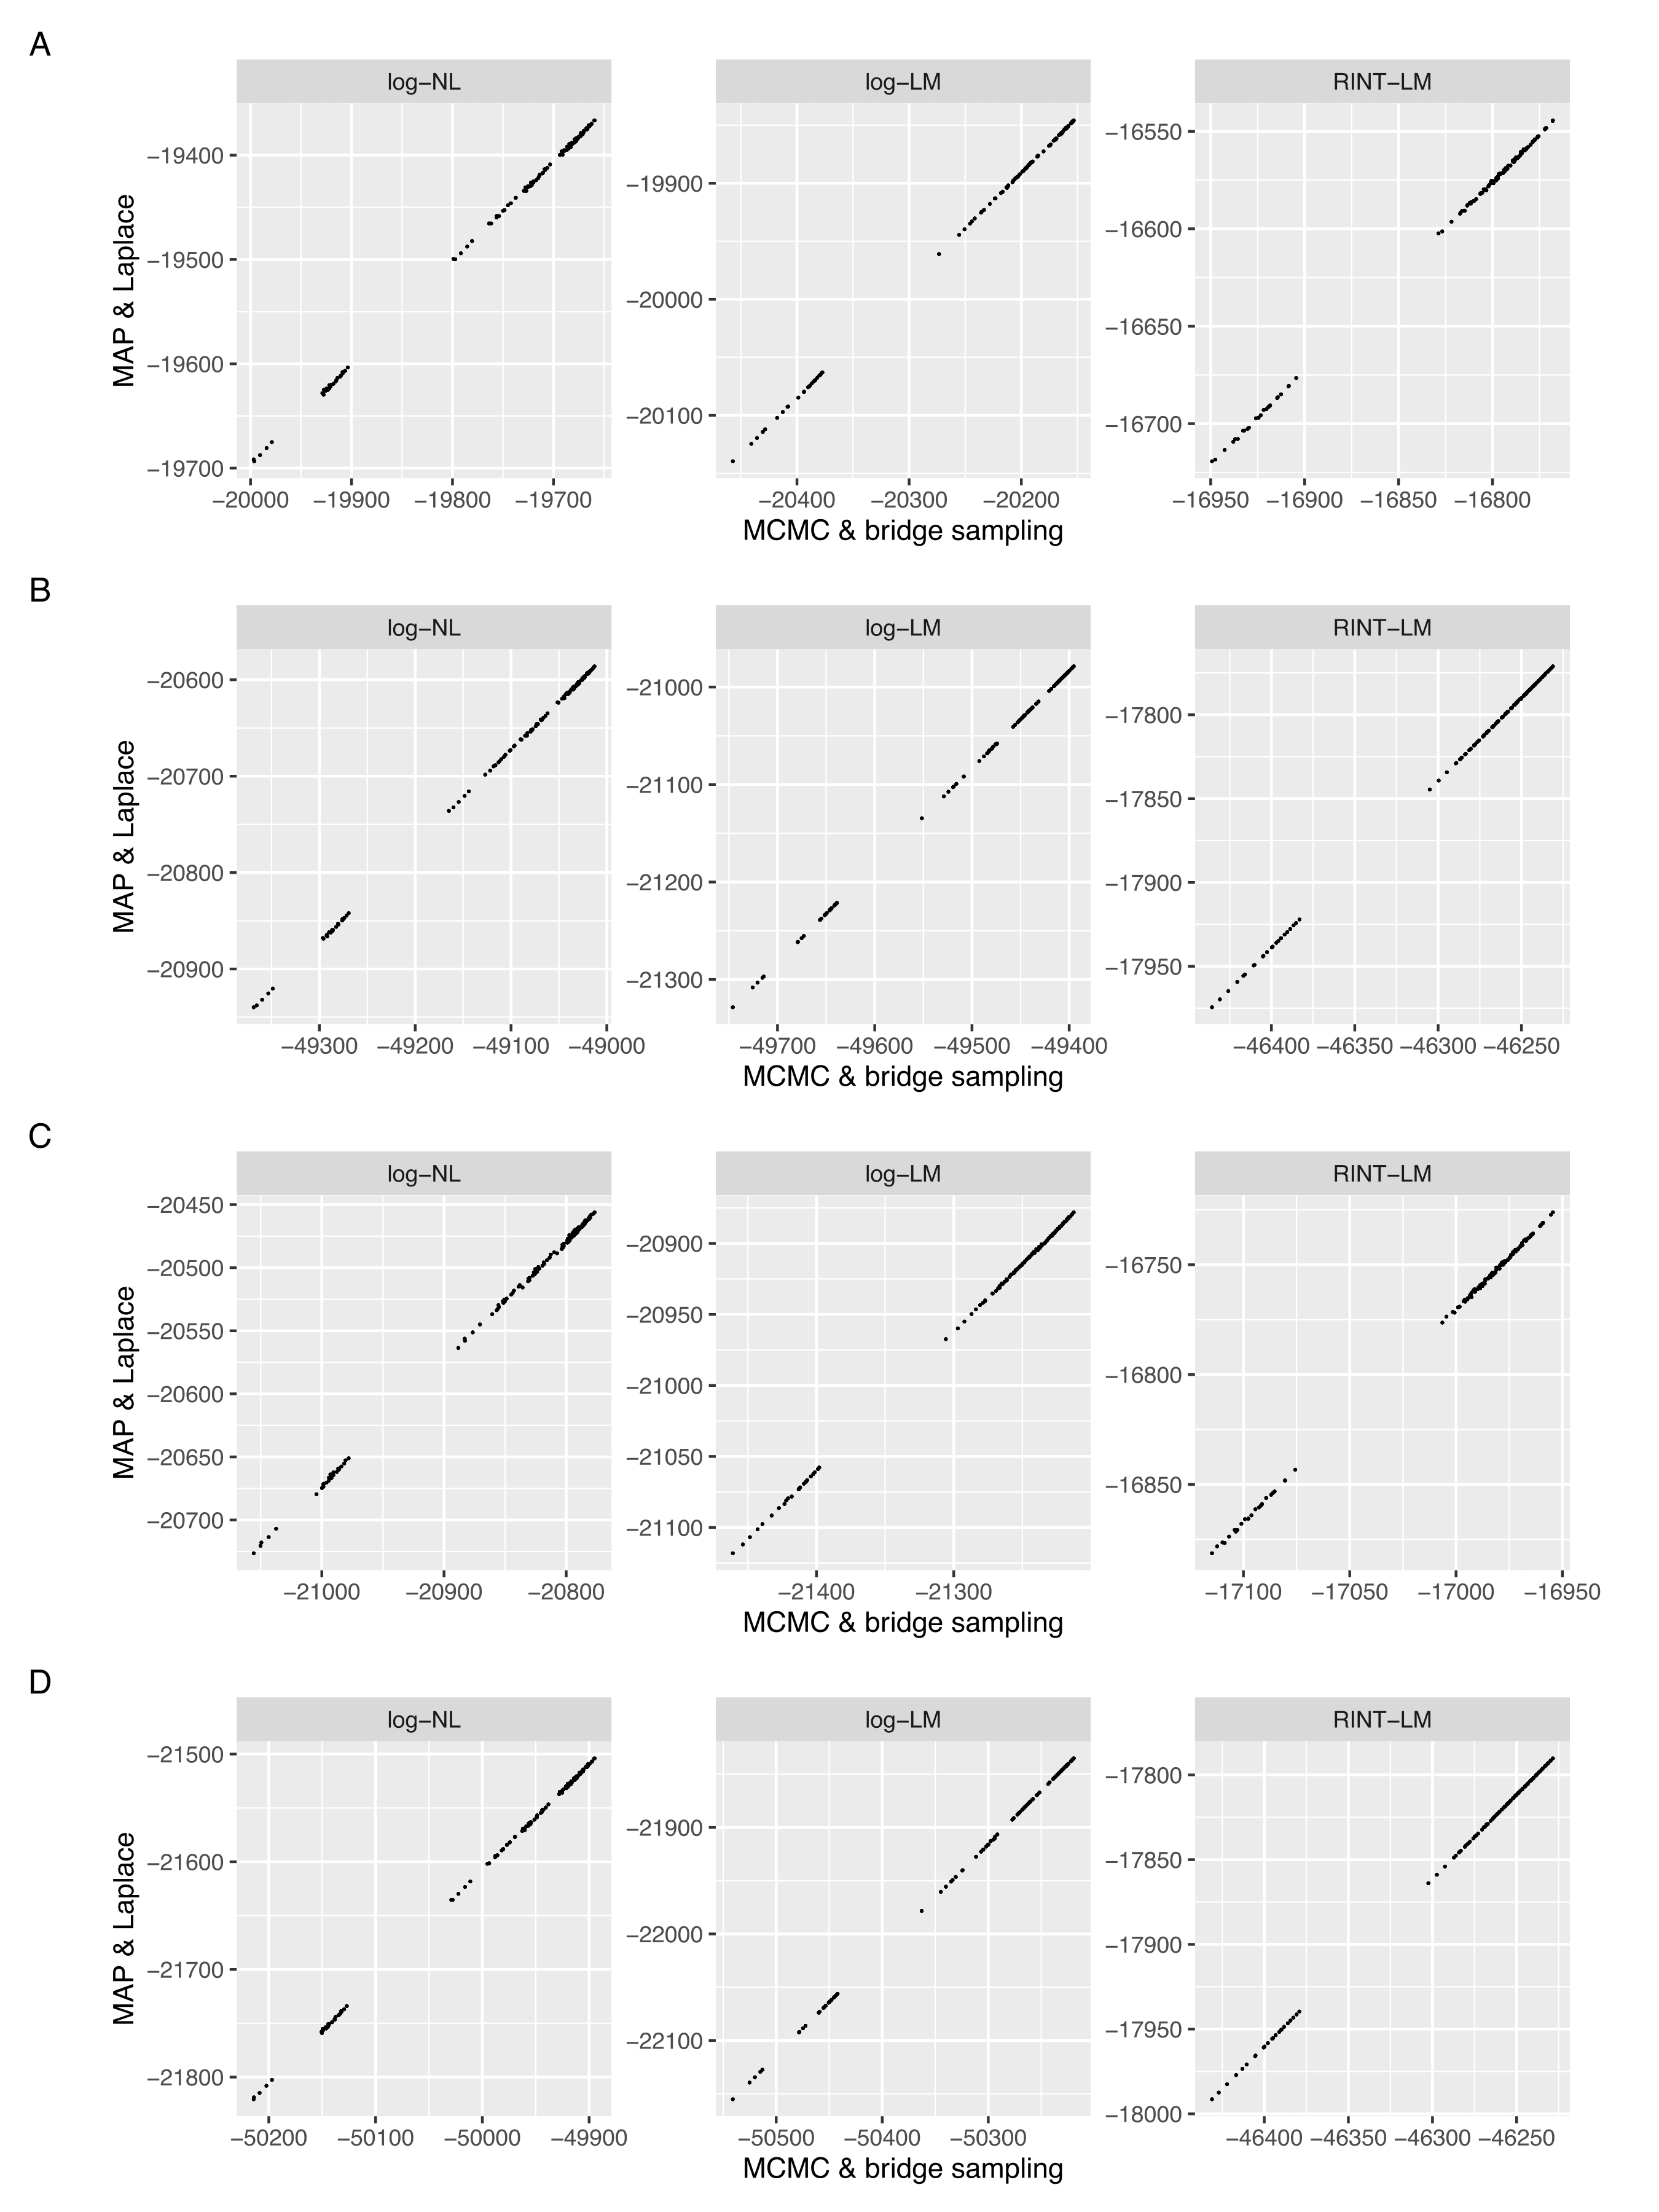
\includegraphics[width=0.8\textwidth]{png/sim_compare_sum_lnpy.png}
\end{center}  
\caption{
  {\bf
    S10 Fig.
    Comparison of the sum of the $\log$ of marginal likelihood across combinations of hyperparameter values between two computational approaches for $\log$-NL, $\log$-LM, and RINT-LM with and without donor random effects.}
Scatter plots comparing results obtained by MCMC followed by bridge sampling and those obtained by MAP estimation followed by Laplace approximation. Each point represents the $\log$ of the marginal likelihood summed over 80 feature-SNP pairs.
The values are compared across 125 combinations of the hyperparameter values (see \stext for details).
}
\label{s-fig:sim-compare-sum}
\end{figure}

\begin{figure}[!ht]
\begin{center}
  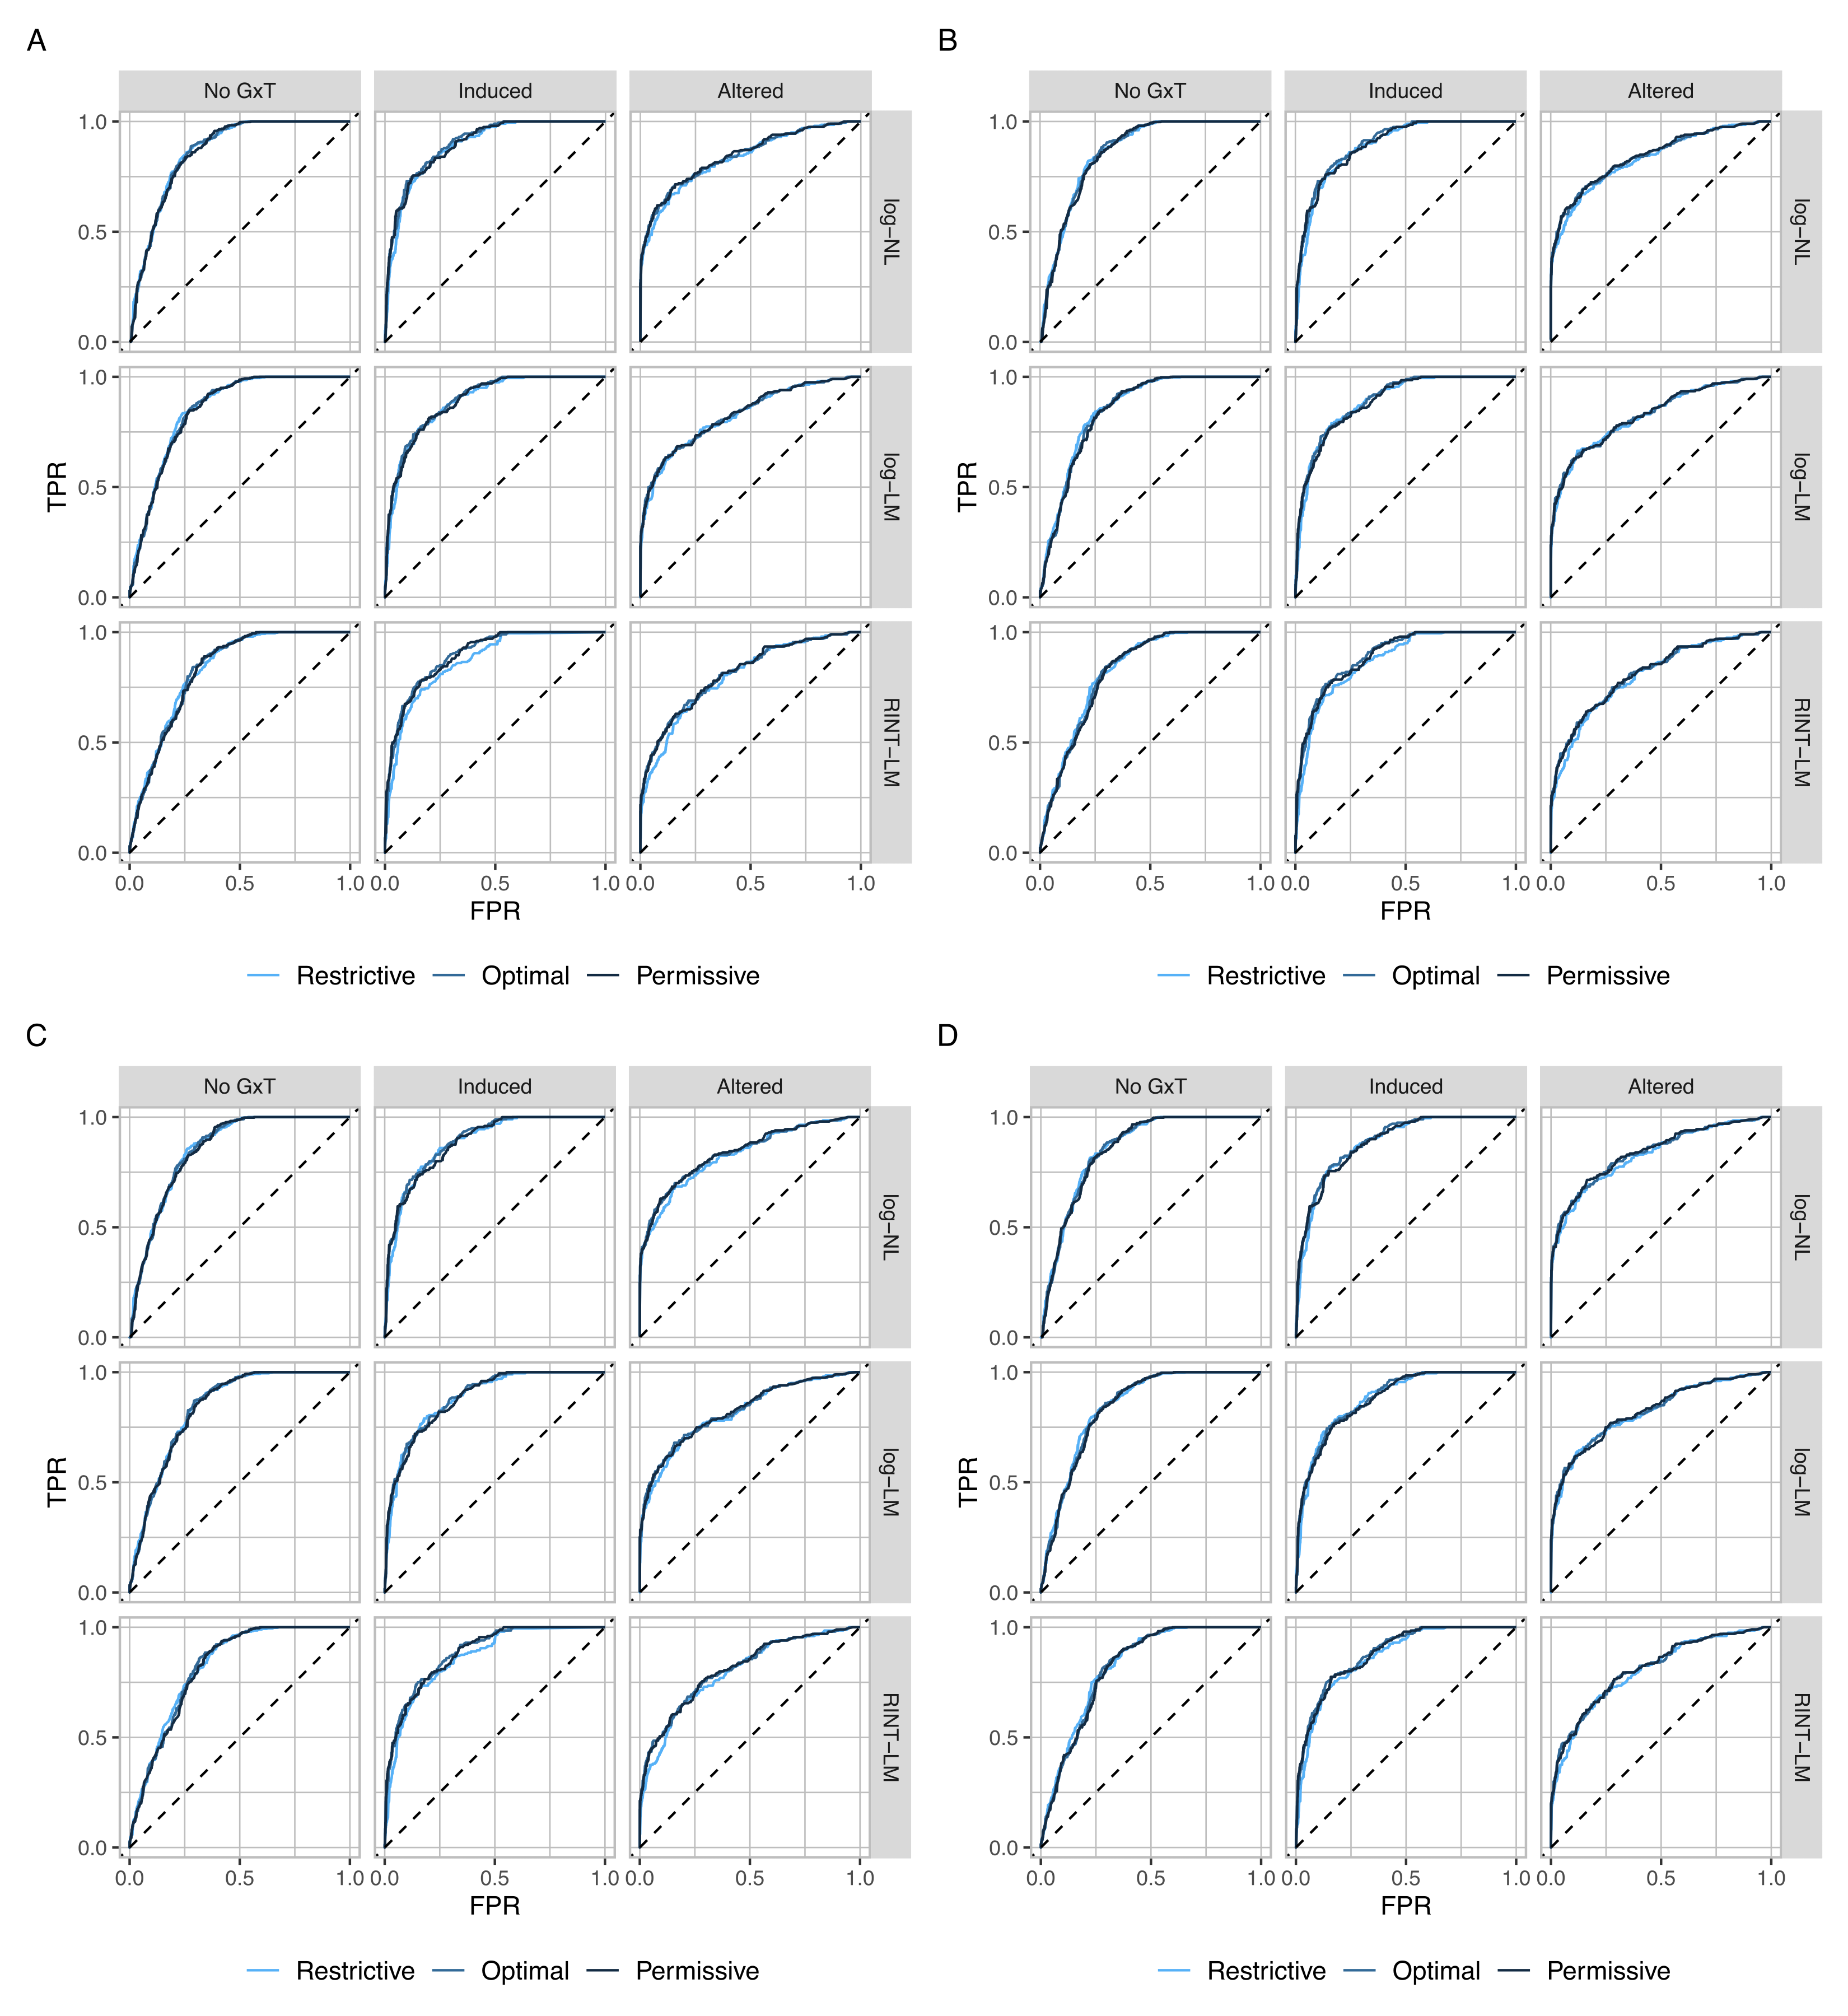
\includegraphics[width=1\textwidth]{png/sim_rocc_effect_mcmc_bs.png}
\end{center}  
\caption{
  {\bf
    S11 Fig.
    ROC curves assessing the impact of the effect prior on the performance of BMS using MCMC and bridge sampling.}
The colors represent varying hyper parameter values (see
\stext). The panels \textbf{A} to \textbf{D} show results in scenarios 1 to 4, which are described in the legend to
\sfigroccmcmc. In each panel, the rows and columns represent modeling approaches and aggregated categories, respectively.
}
\label{s-fig:sim-rocc-effect-mcmc}
\end{figure}

\begin{figure}[!ht]
\begin{center}
  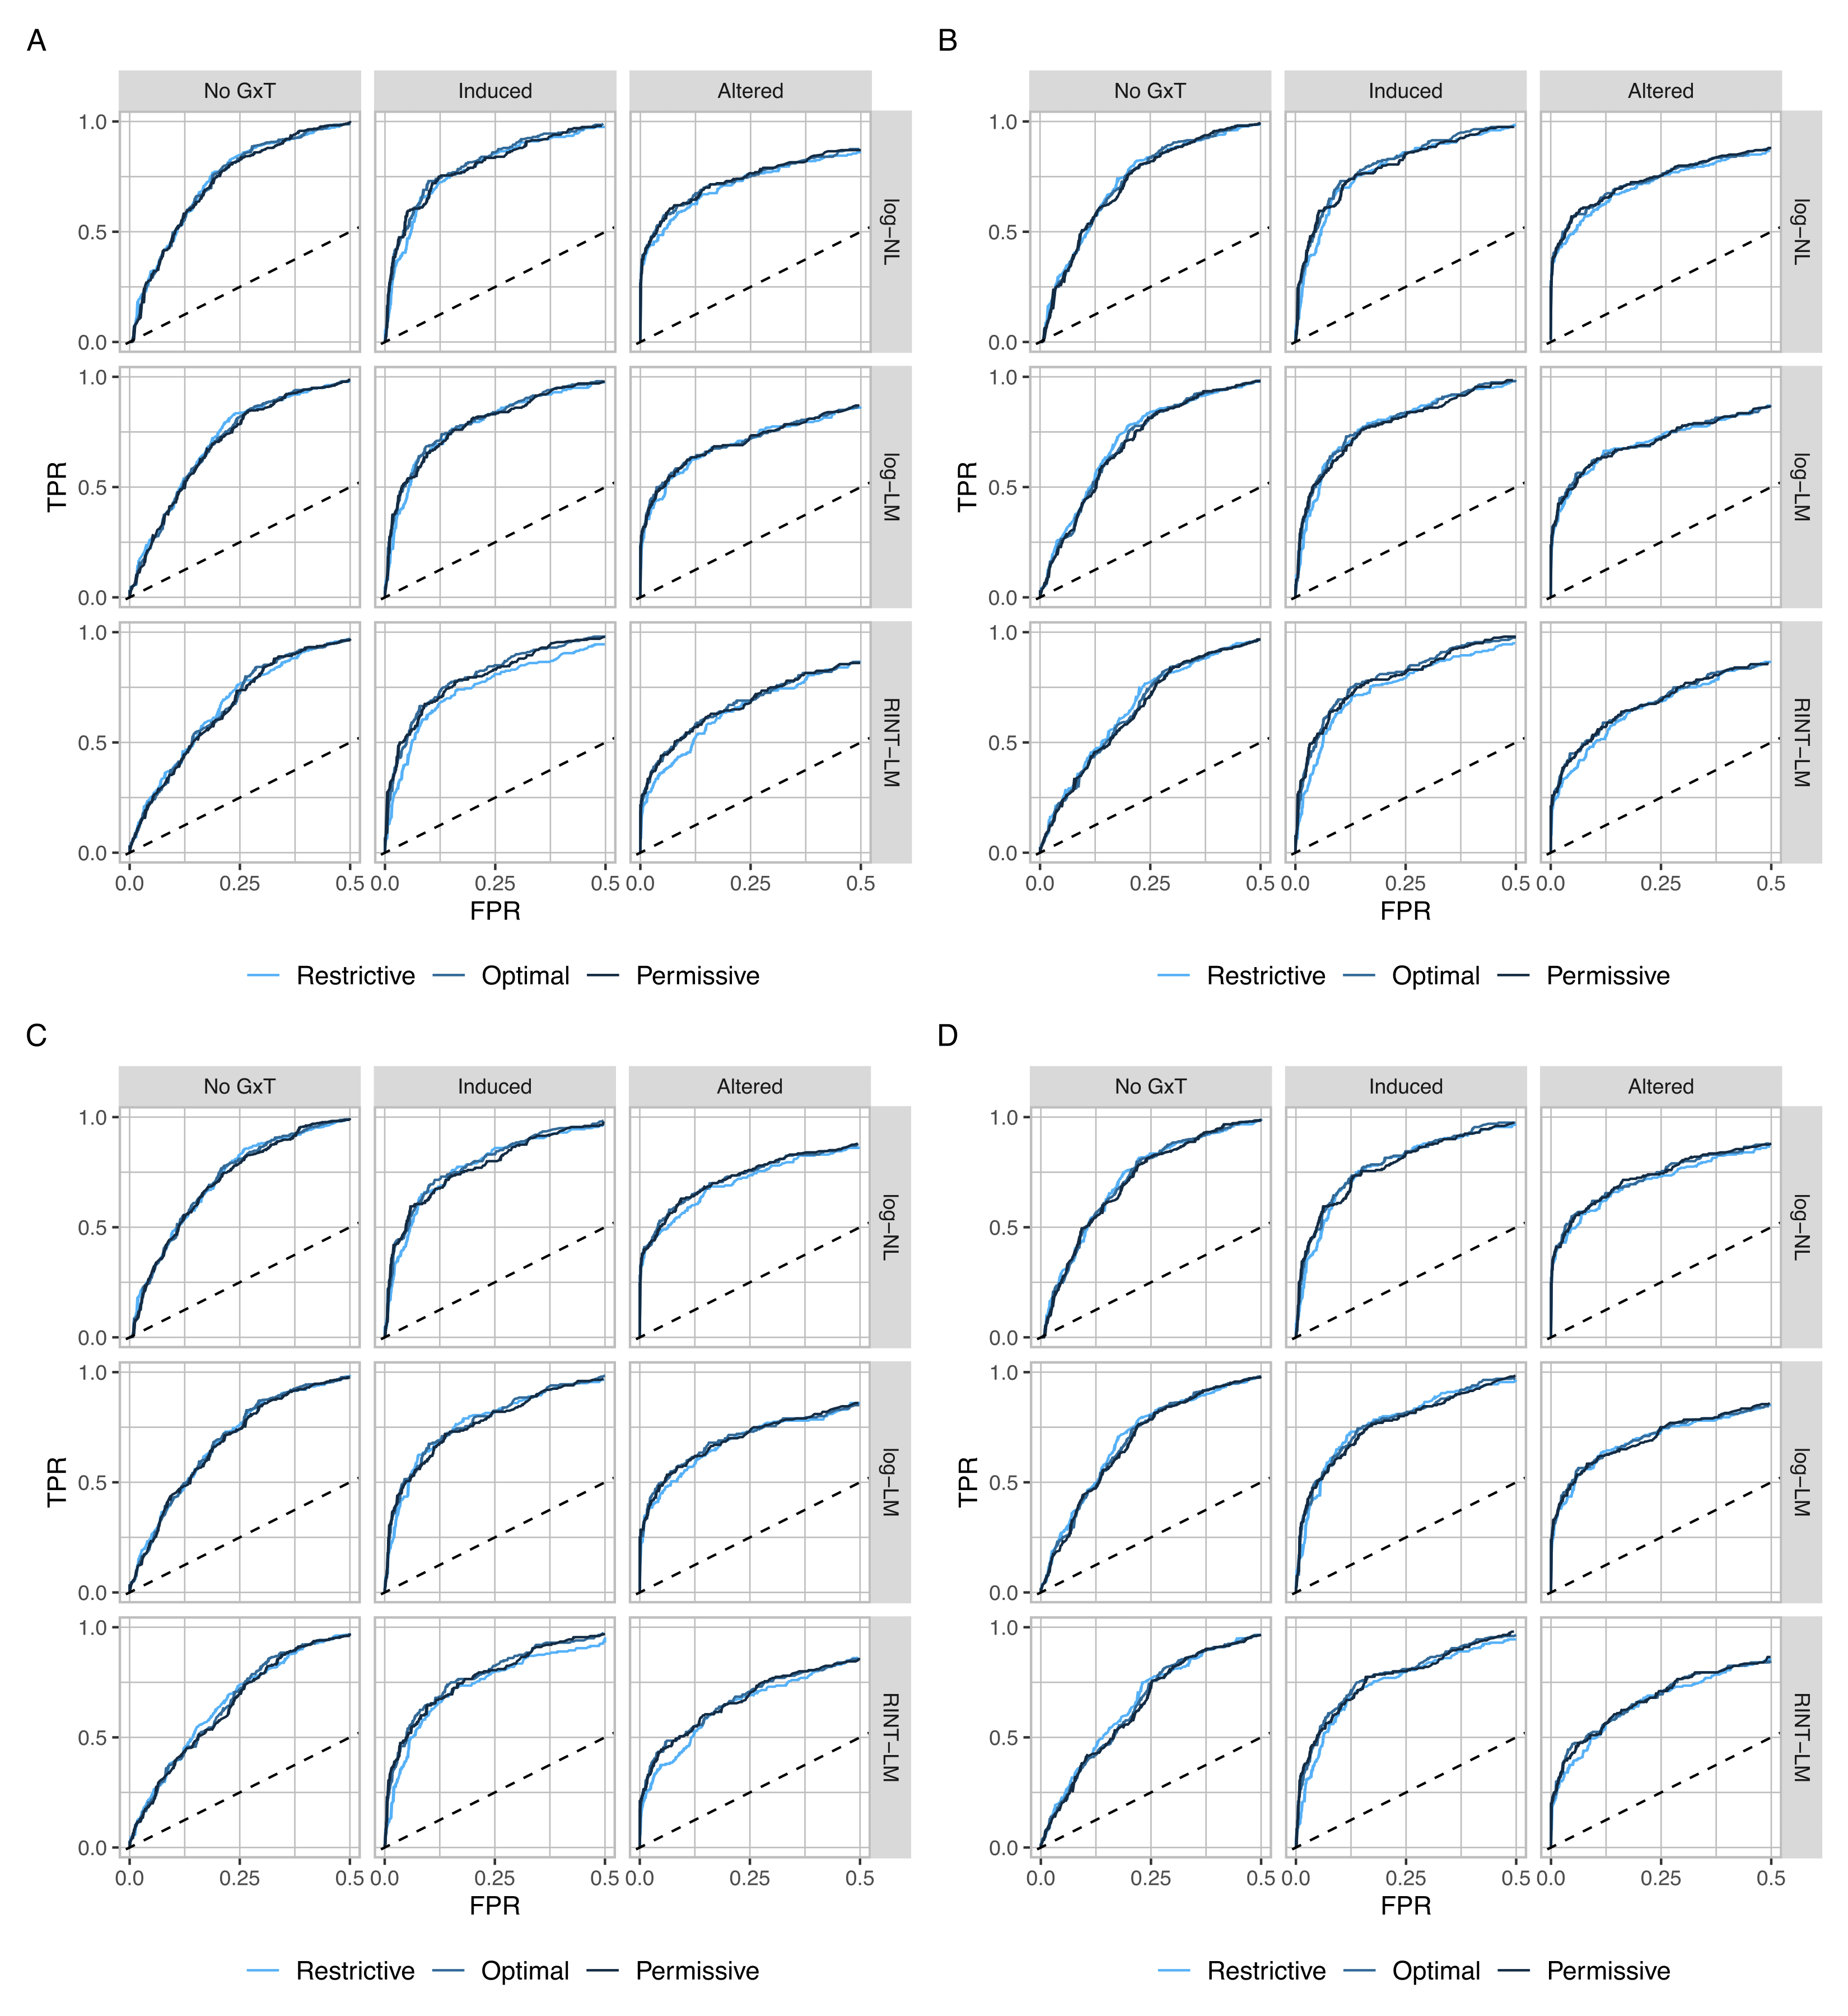
\includegraphics[width=1\textwidth]{png/sim_procc_effect_mcmc_bs.png}
\end{center}  
\caption{
  {\bf
    S12 Fig.
    Partial ROC curves assessing the impact of the effect prior on the performance of BMS using MCMC and bridge sampling.}
The colors represent varying hyper parameter values (see
\stext). The panels \textbf{A} to \textbf{D} show results in scenarios 1 to 4, which are described in the legend to \stext. In each panel, the rows and columns represent modeling approaches and aggregated categories, respectively.
}    
\label{s-fig:sim-procc-effect-mcmc}
\end{figure}

\begin{figure}[!ht]
\begin{center}
  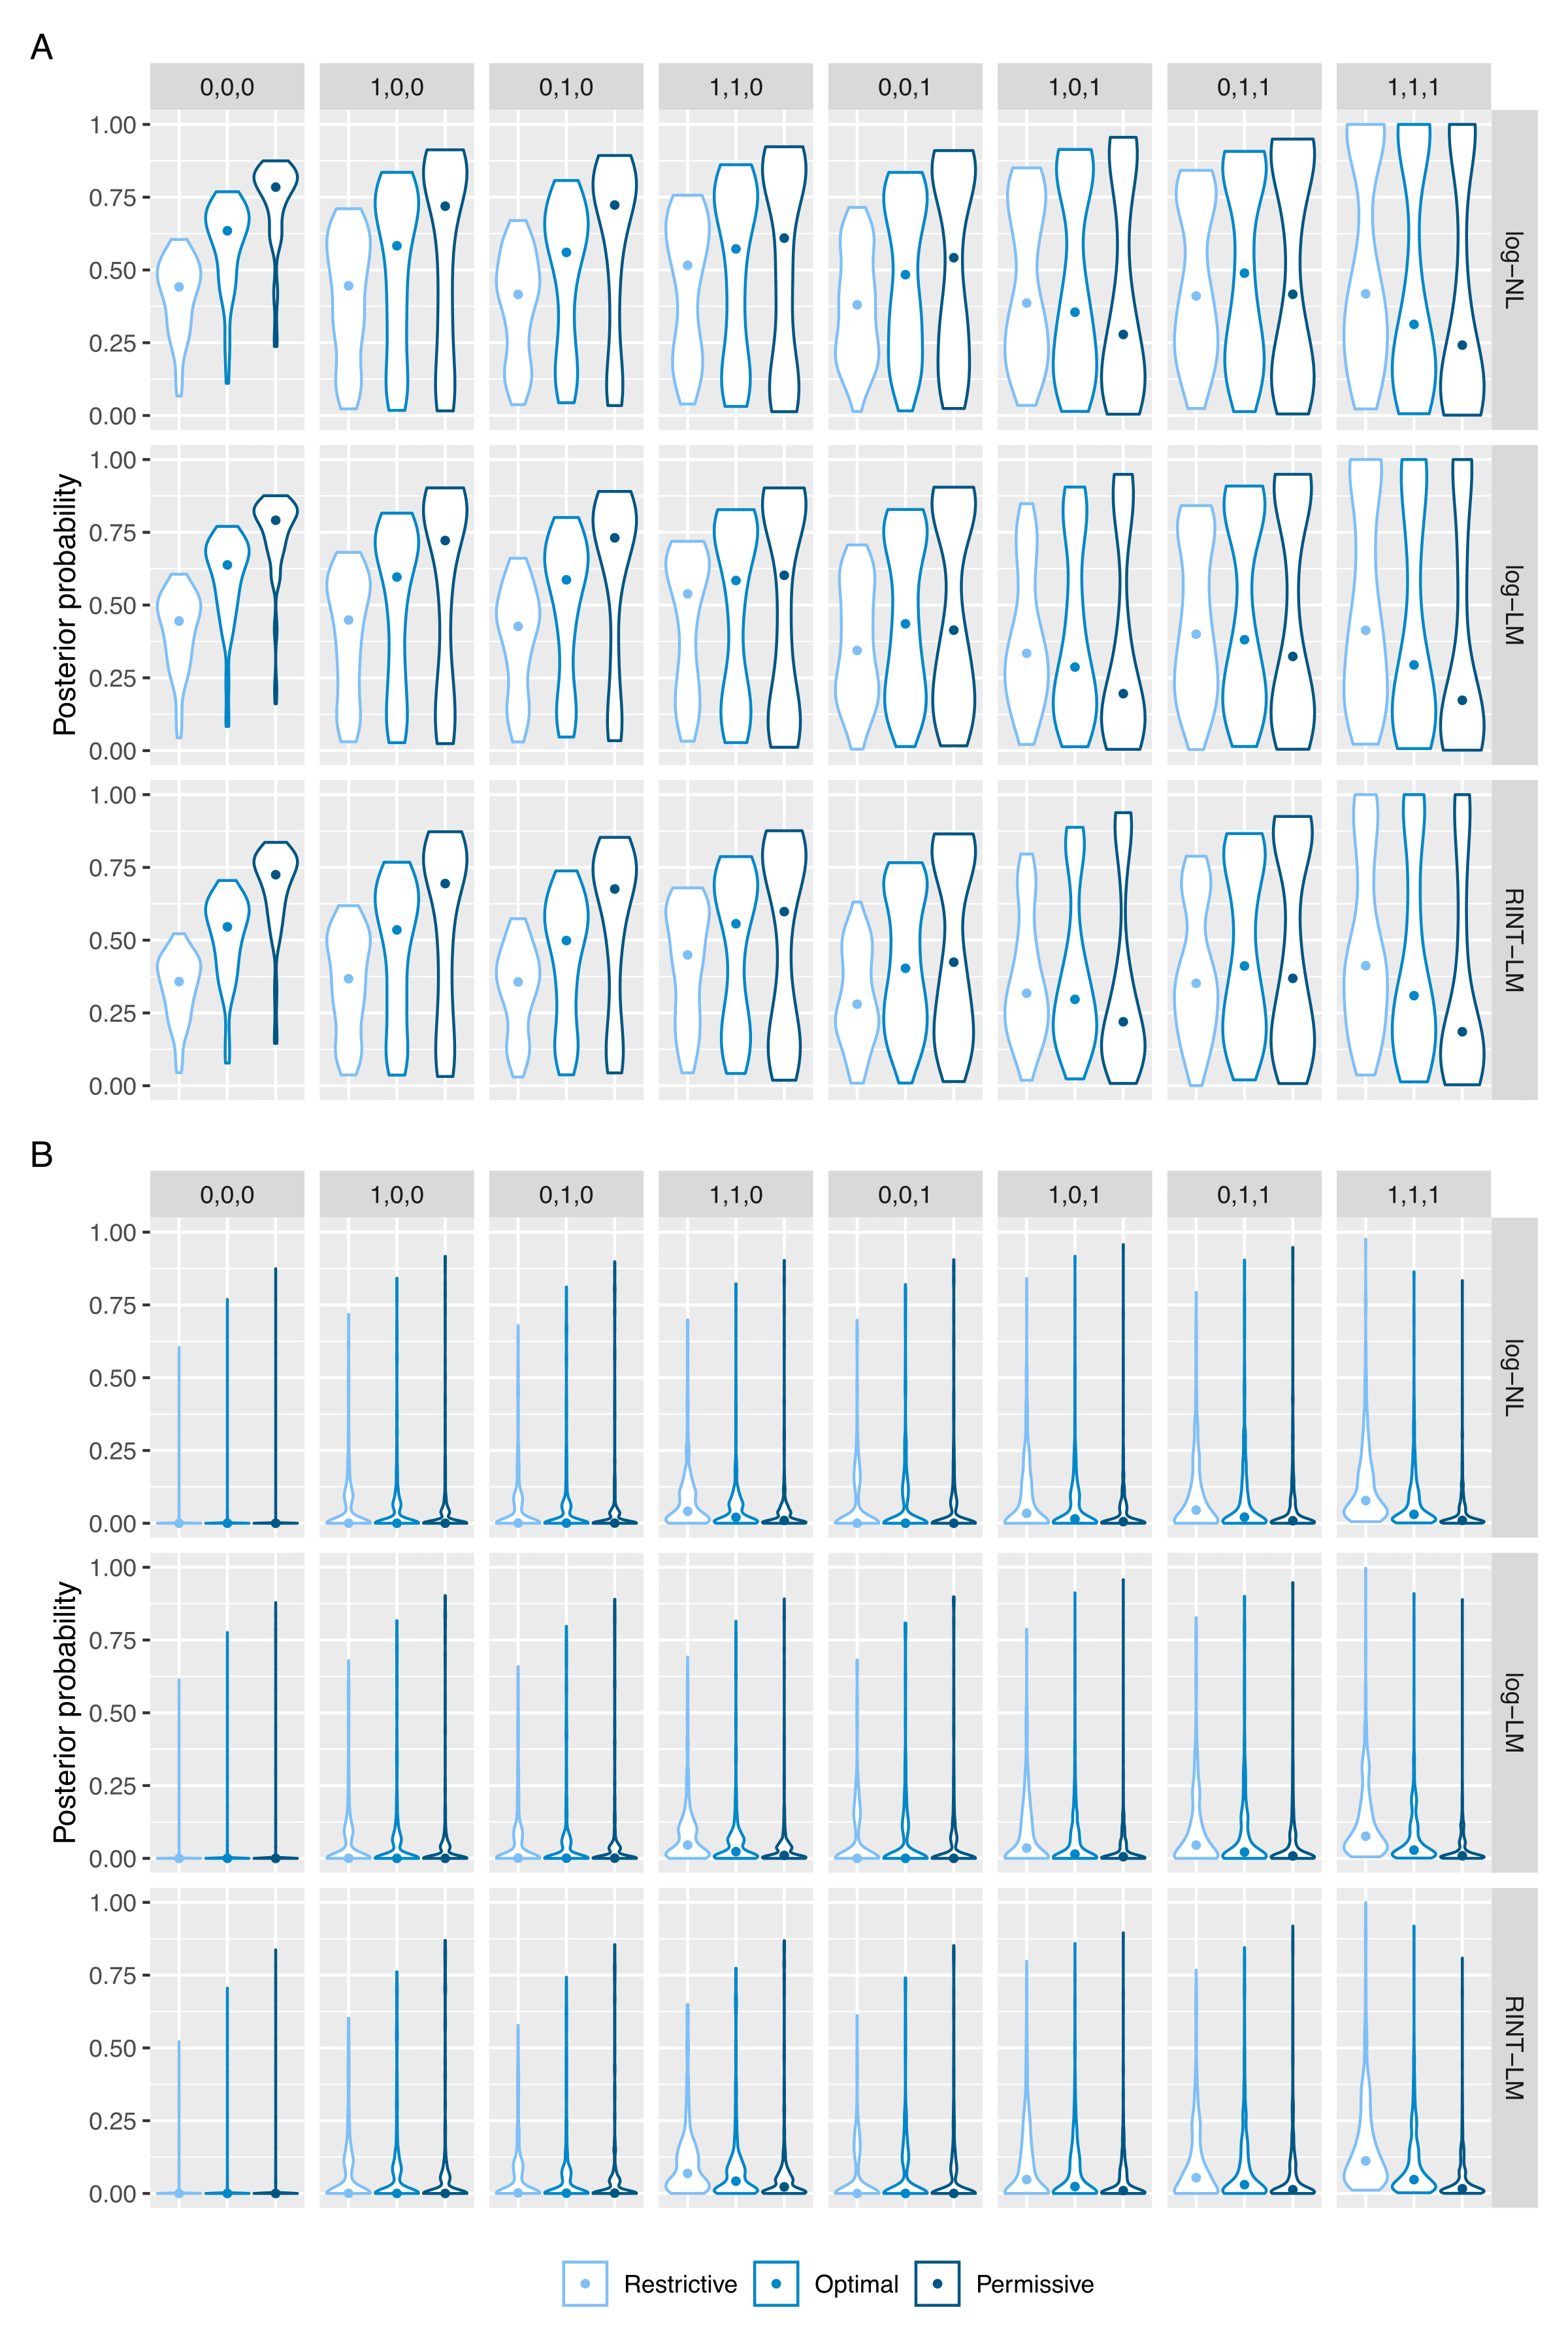
\includegraphics[width=0.75\textwidth]{png/sim_vln_effect_mcmc_bs_noranef_noranef.png}
\end{center}  
\caption{
  {\bf
    S13 Fig.
    Assessing the impact of the effect prior on the posterior probability of the correct and incorrect models from analyses without random effect using MCMC and bridge sampling.}
Violin plots showing the distribution of posterior probability of the correct (\textbf{A}) and incorrect (\textbf{B}) models for each of the eight model categories with varying hyper parameter values (see \stext). The closed circles represent median values. Shown is the results in scenario 1, which is described in the legend to \sfigroccmcmc.
}
\label{s-fig:sim-effect-mcmc-noranef-noranef}
\end{figure}

\begin{figure}[!ht]
\begin{center}
  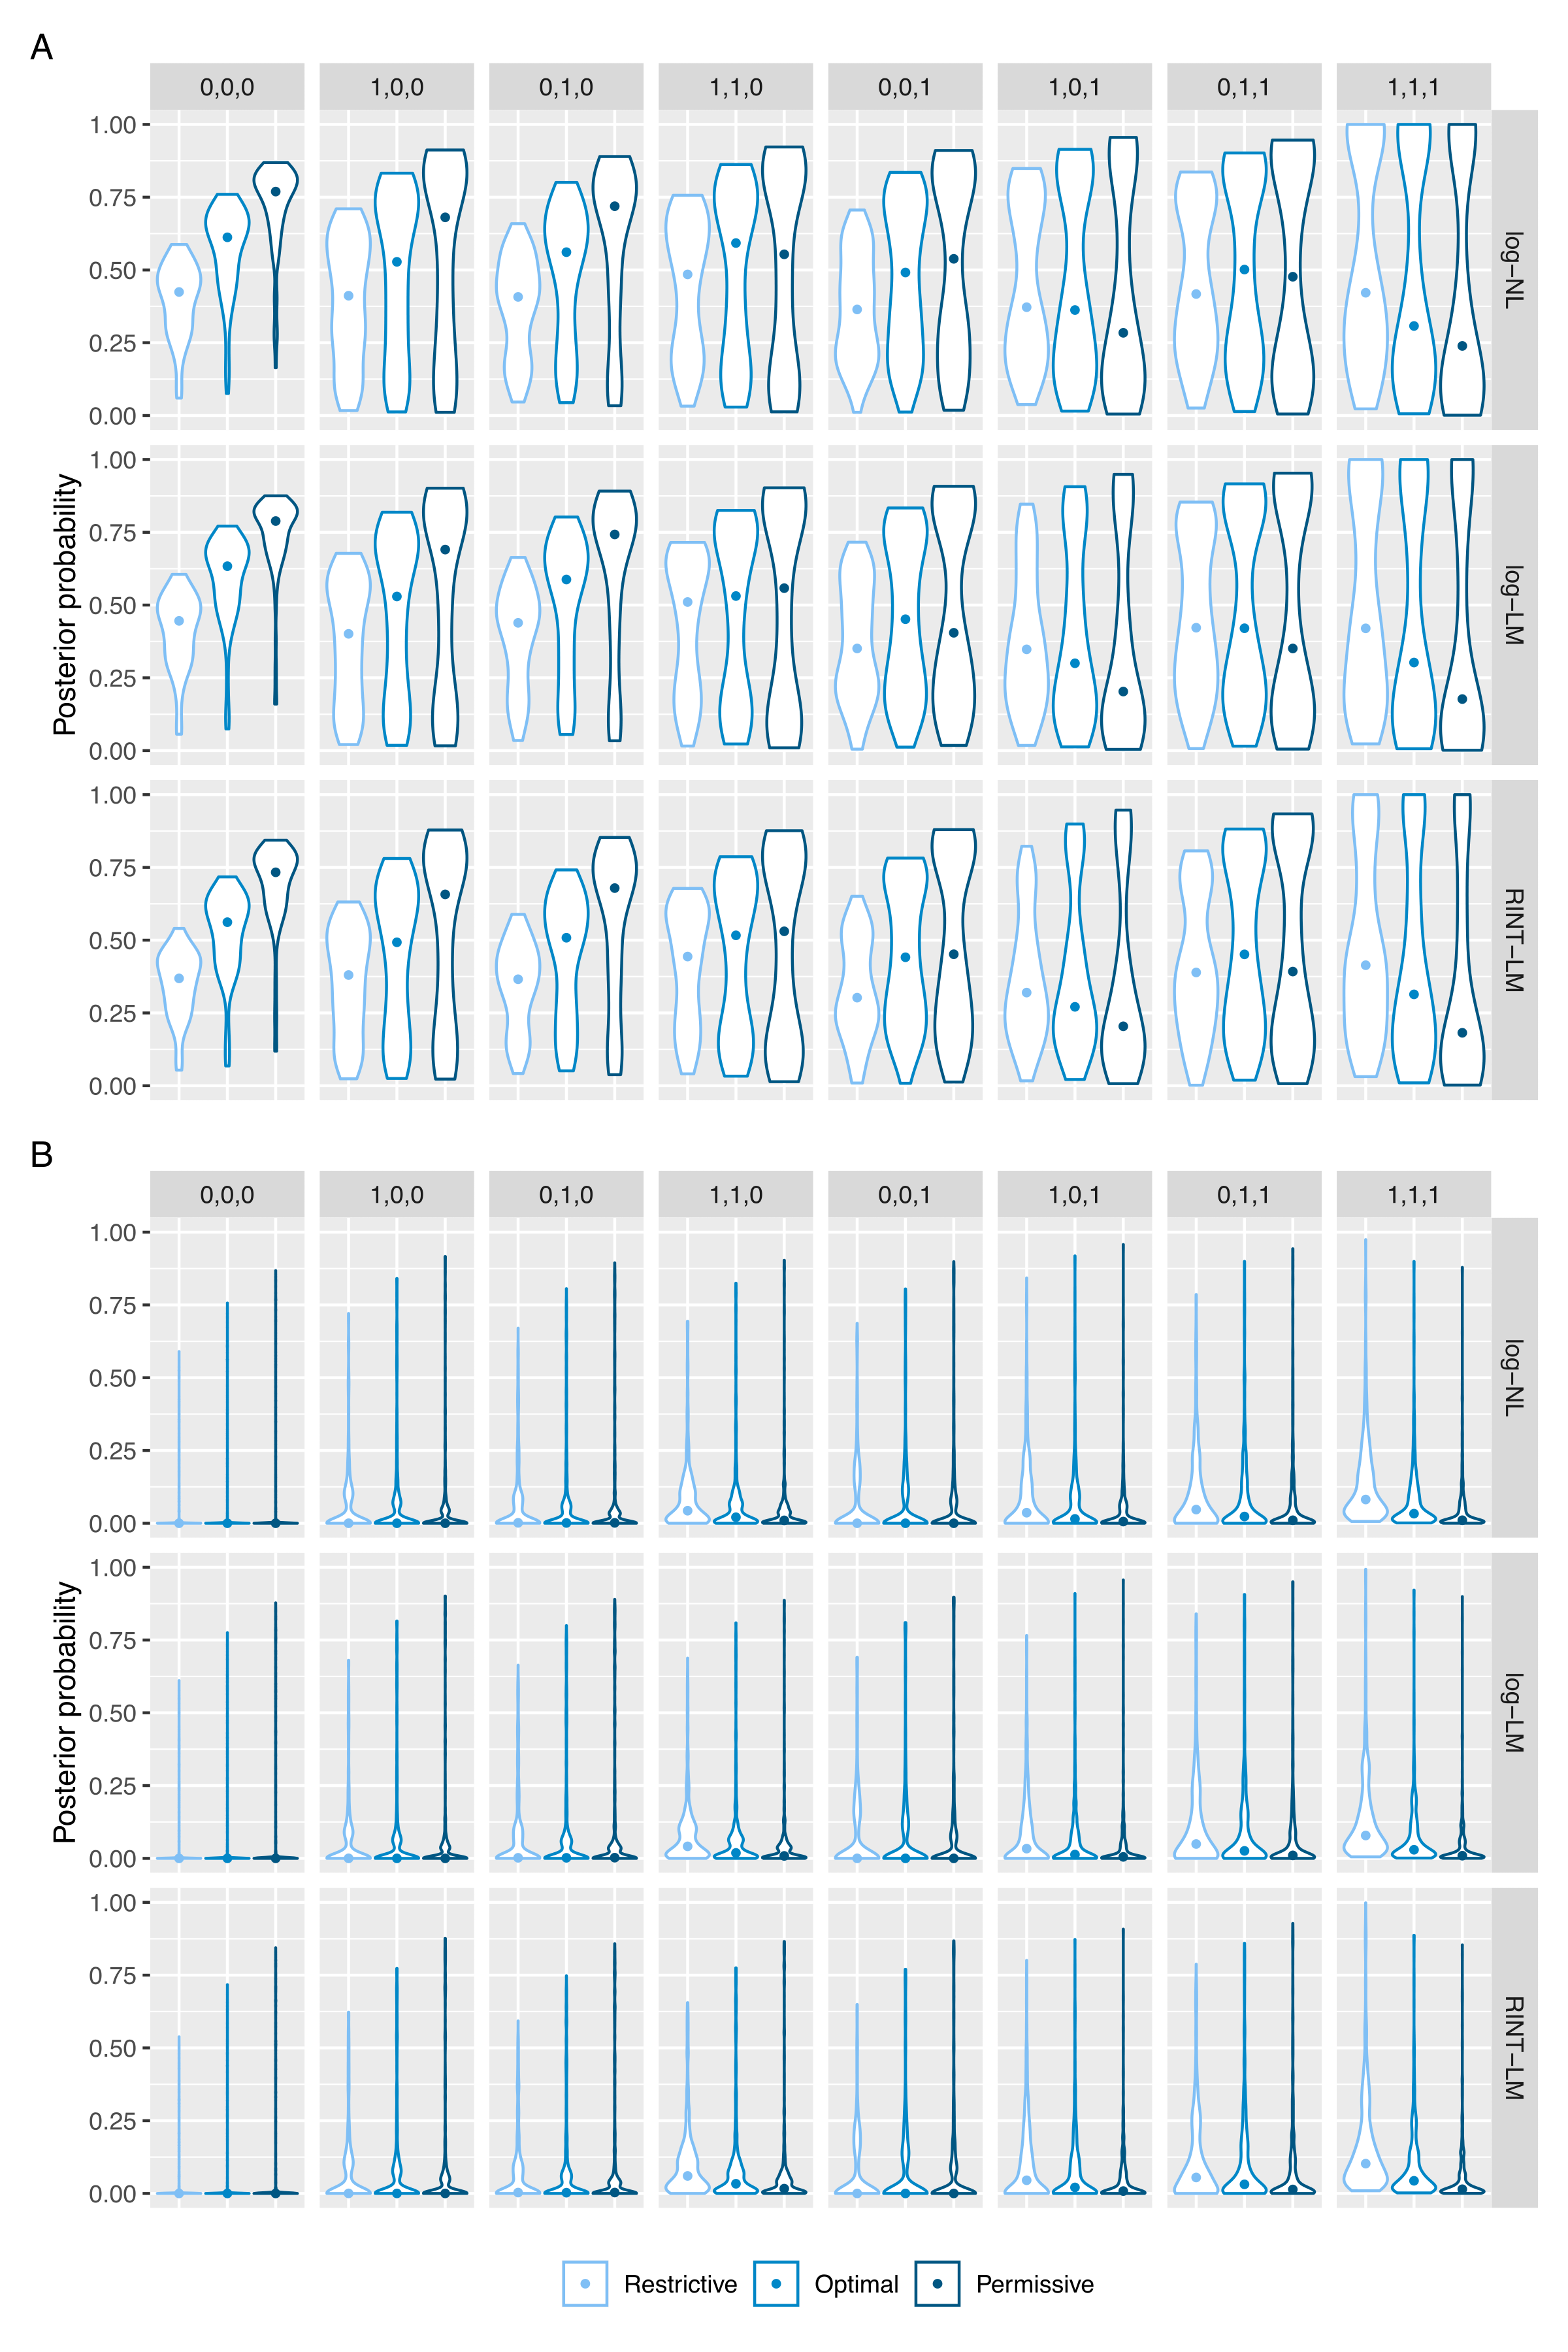
\includegraphics[width=0.75\textwidth]{png/sim_vln_effect_mcmc_bs_noranef_ranef.png}
\end{center}  
\caption{
  {\bf
    S13.2 Fig.
    Assessing the impact of the effect prior on the posterior probability of the correct and incorrect models from analyses with donor random effect in model fitting but not in data generation using MCMC and bridge sampling.}
The same as in \sfigppeffectone but in scenario 2, which is described in the legend to \sfigroccmcmc.
}
\label{s-fig:sim-effect-mcmc-noranef-ranef}
\end{figure}

\begin{figure}[!ht]
\begin{center}
  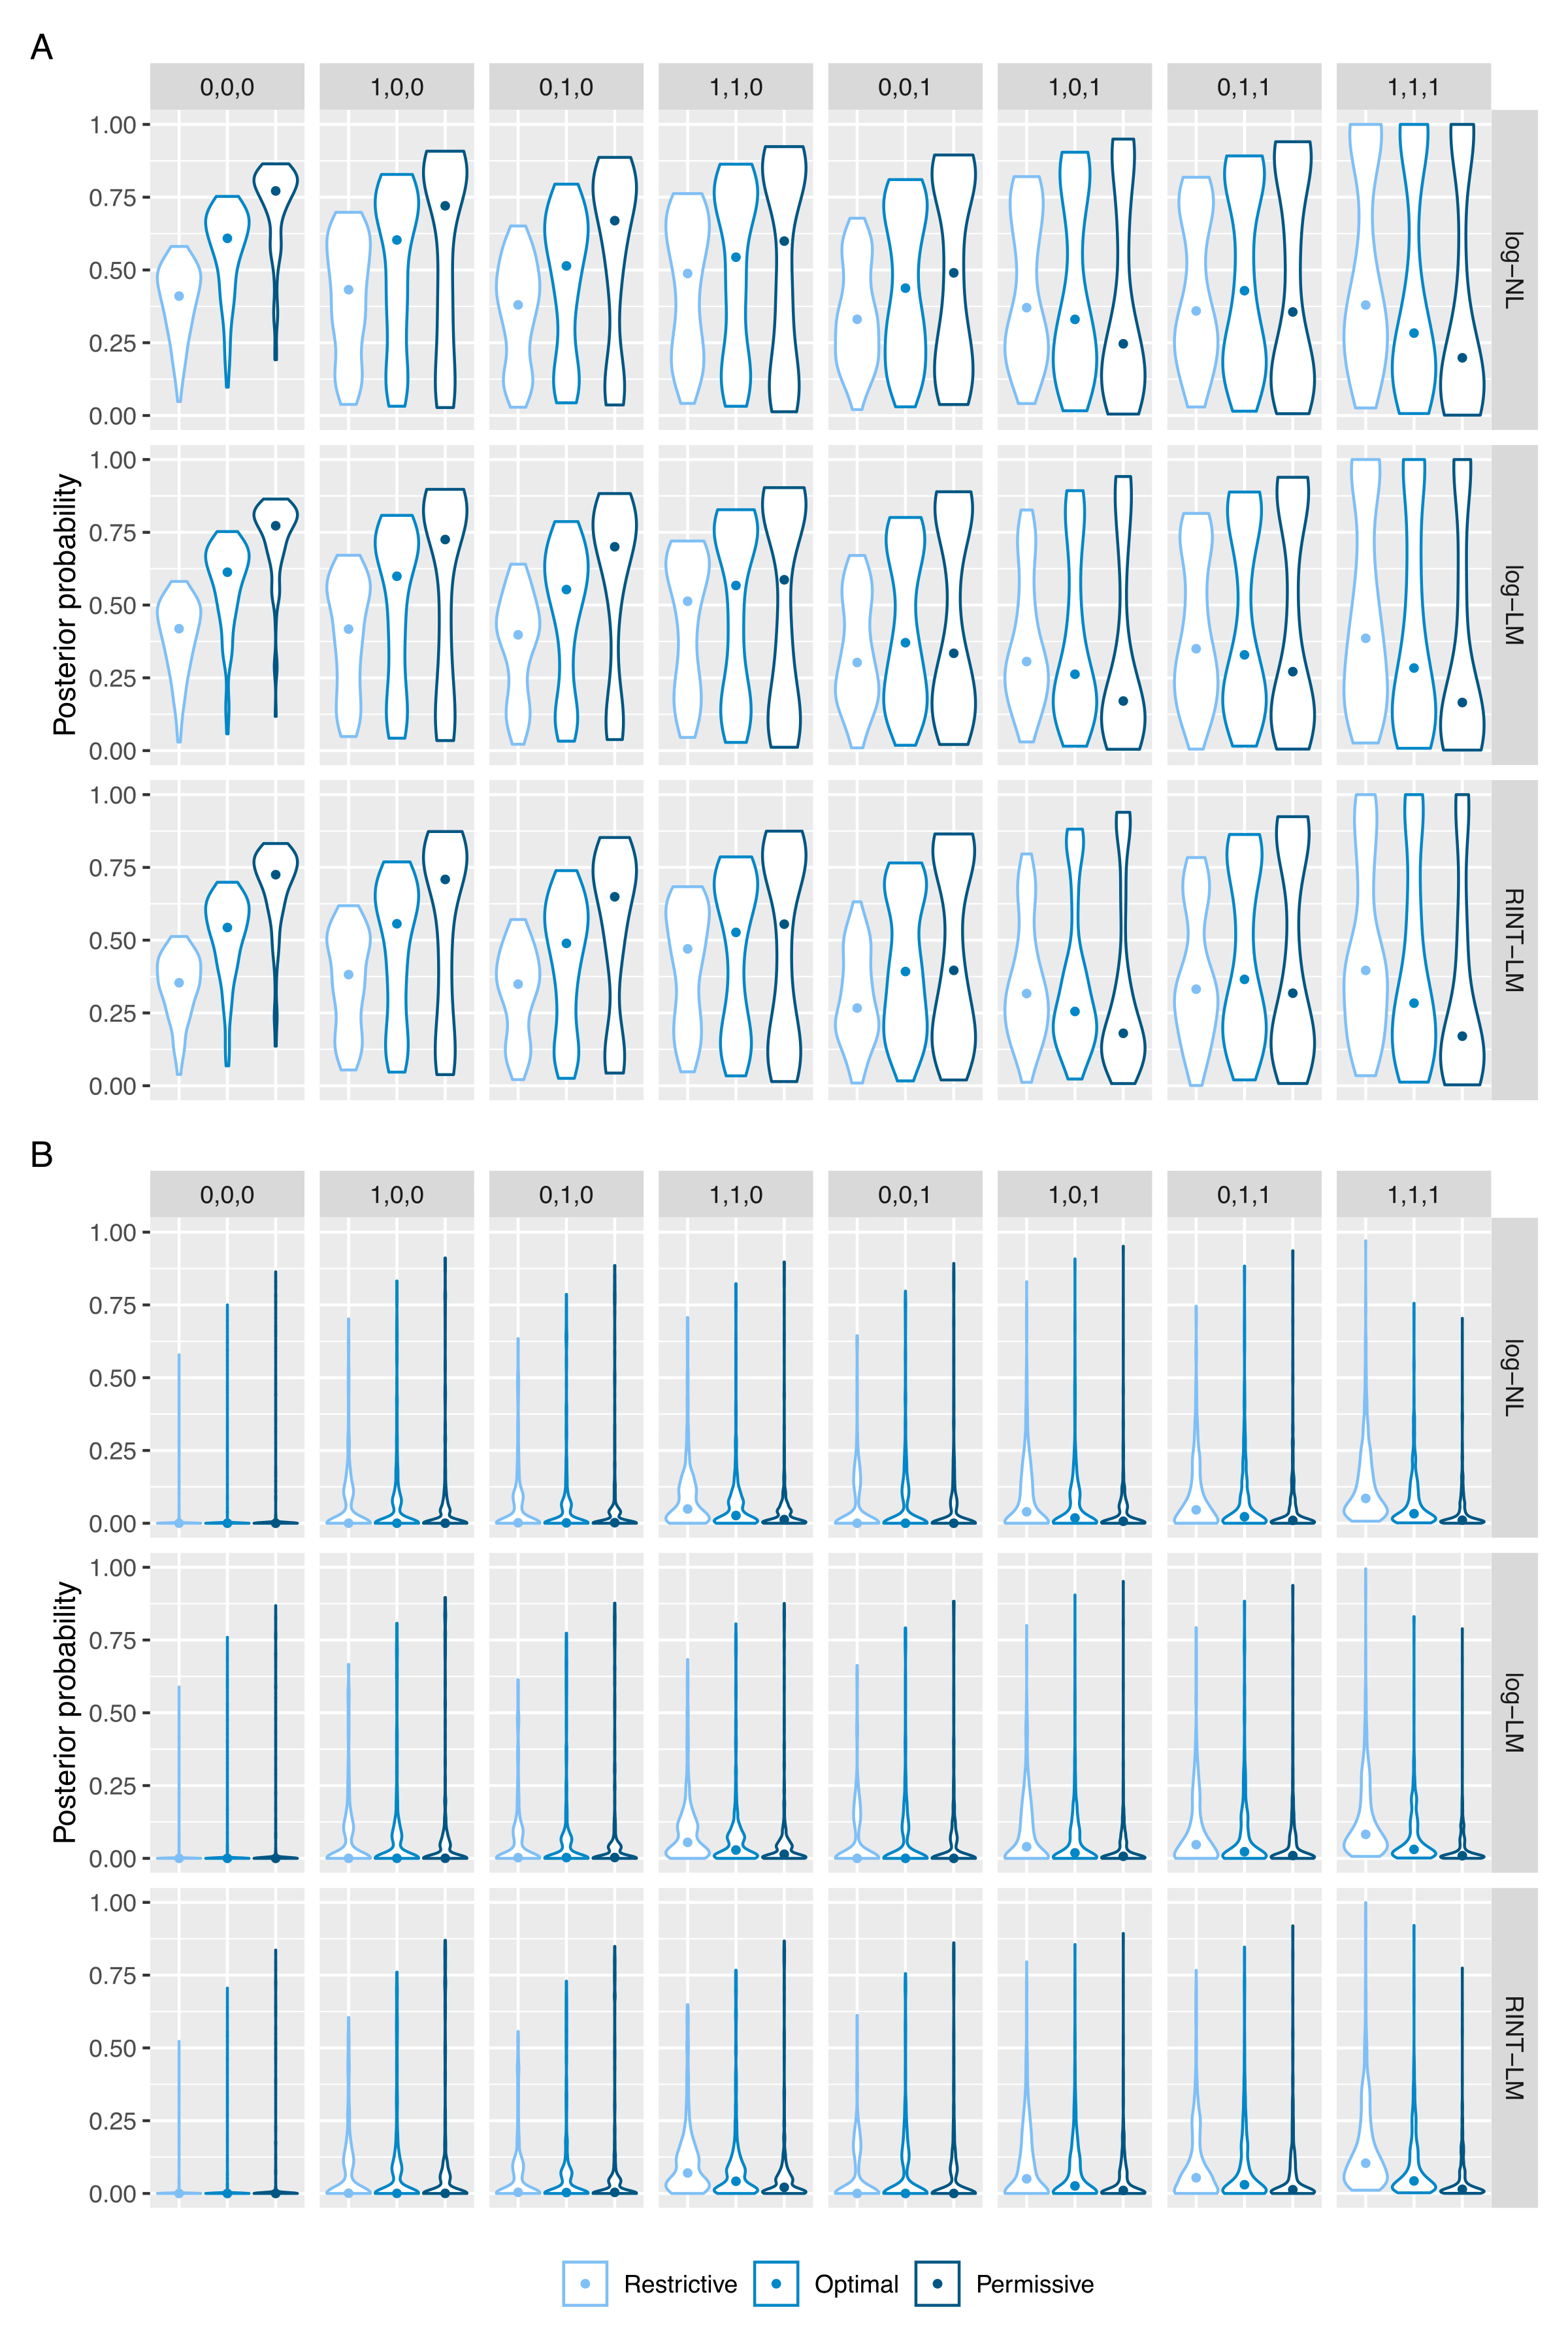
\includegraphics[width=0.75\textwidth]{png/sim_vln_effect_mcmc_bs_ranef_noranef.png}
\end{center}  
\caption{
  {\bf
    S13.3 Fig.
    Assessing the impact of the effect prior on the posterior probability of the correct and incorrect models from analyses with donor random effect in data generation but not in model fitting using MCMC and bridge sampling.}
The same as in \sfigppeffectone but in scenario 3, which is described in the legend to \sfigroccmcmc.
}
\label{s-fig:sim-effect-mcmc-ranef-noranef}
\end{figure}

\begin{figure}[!ht]
\begin{center}
  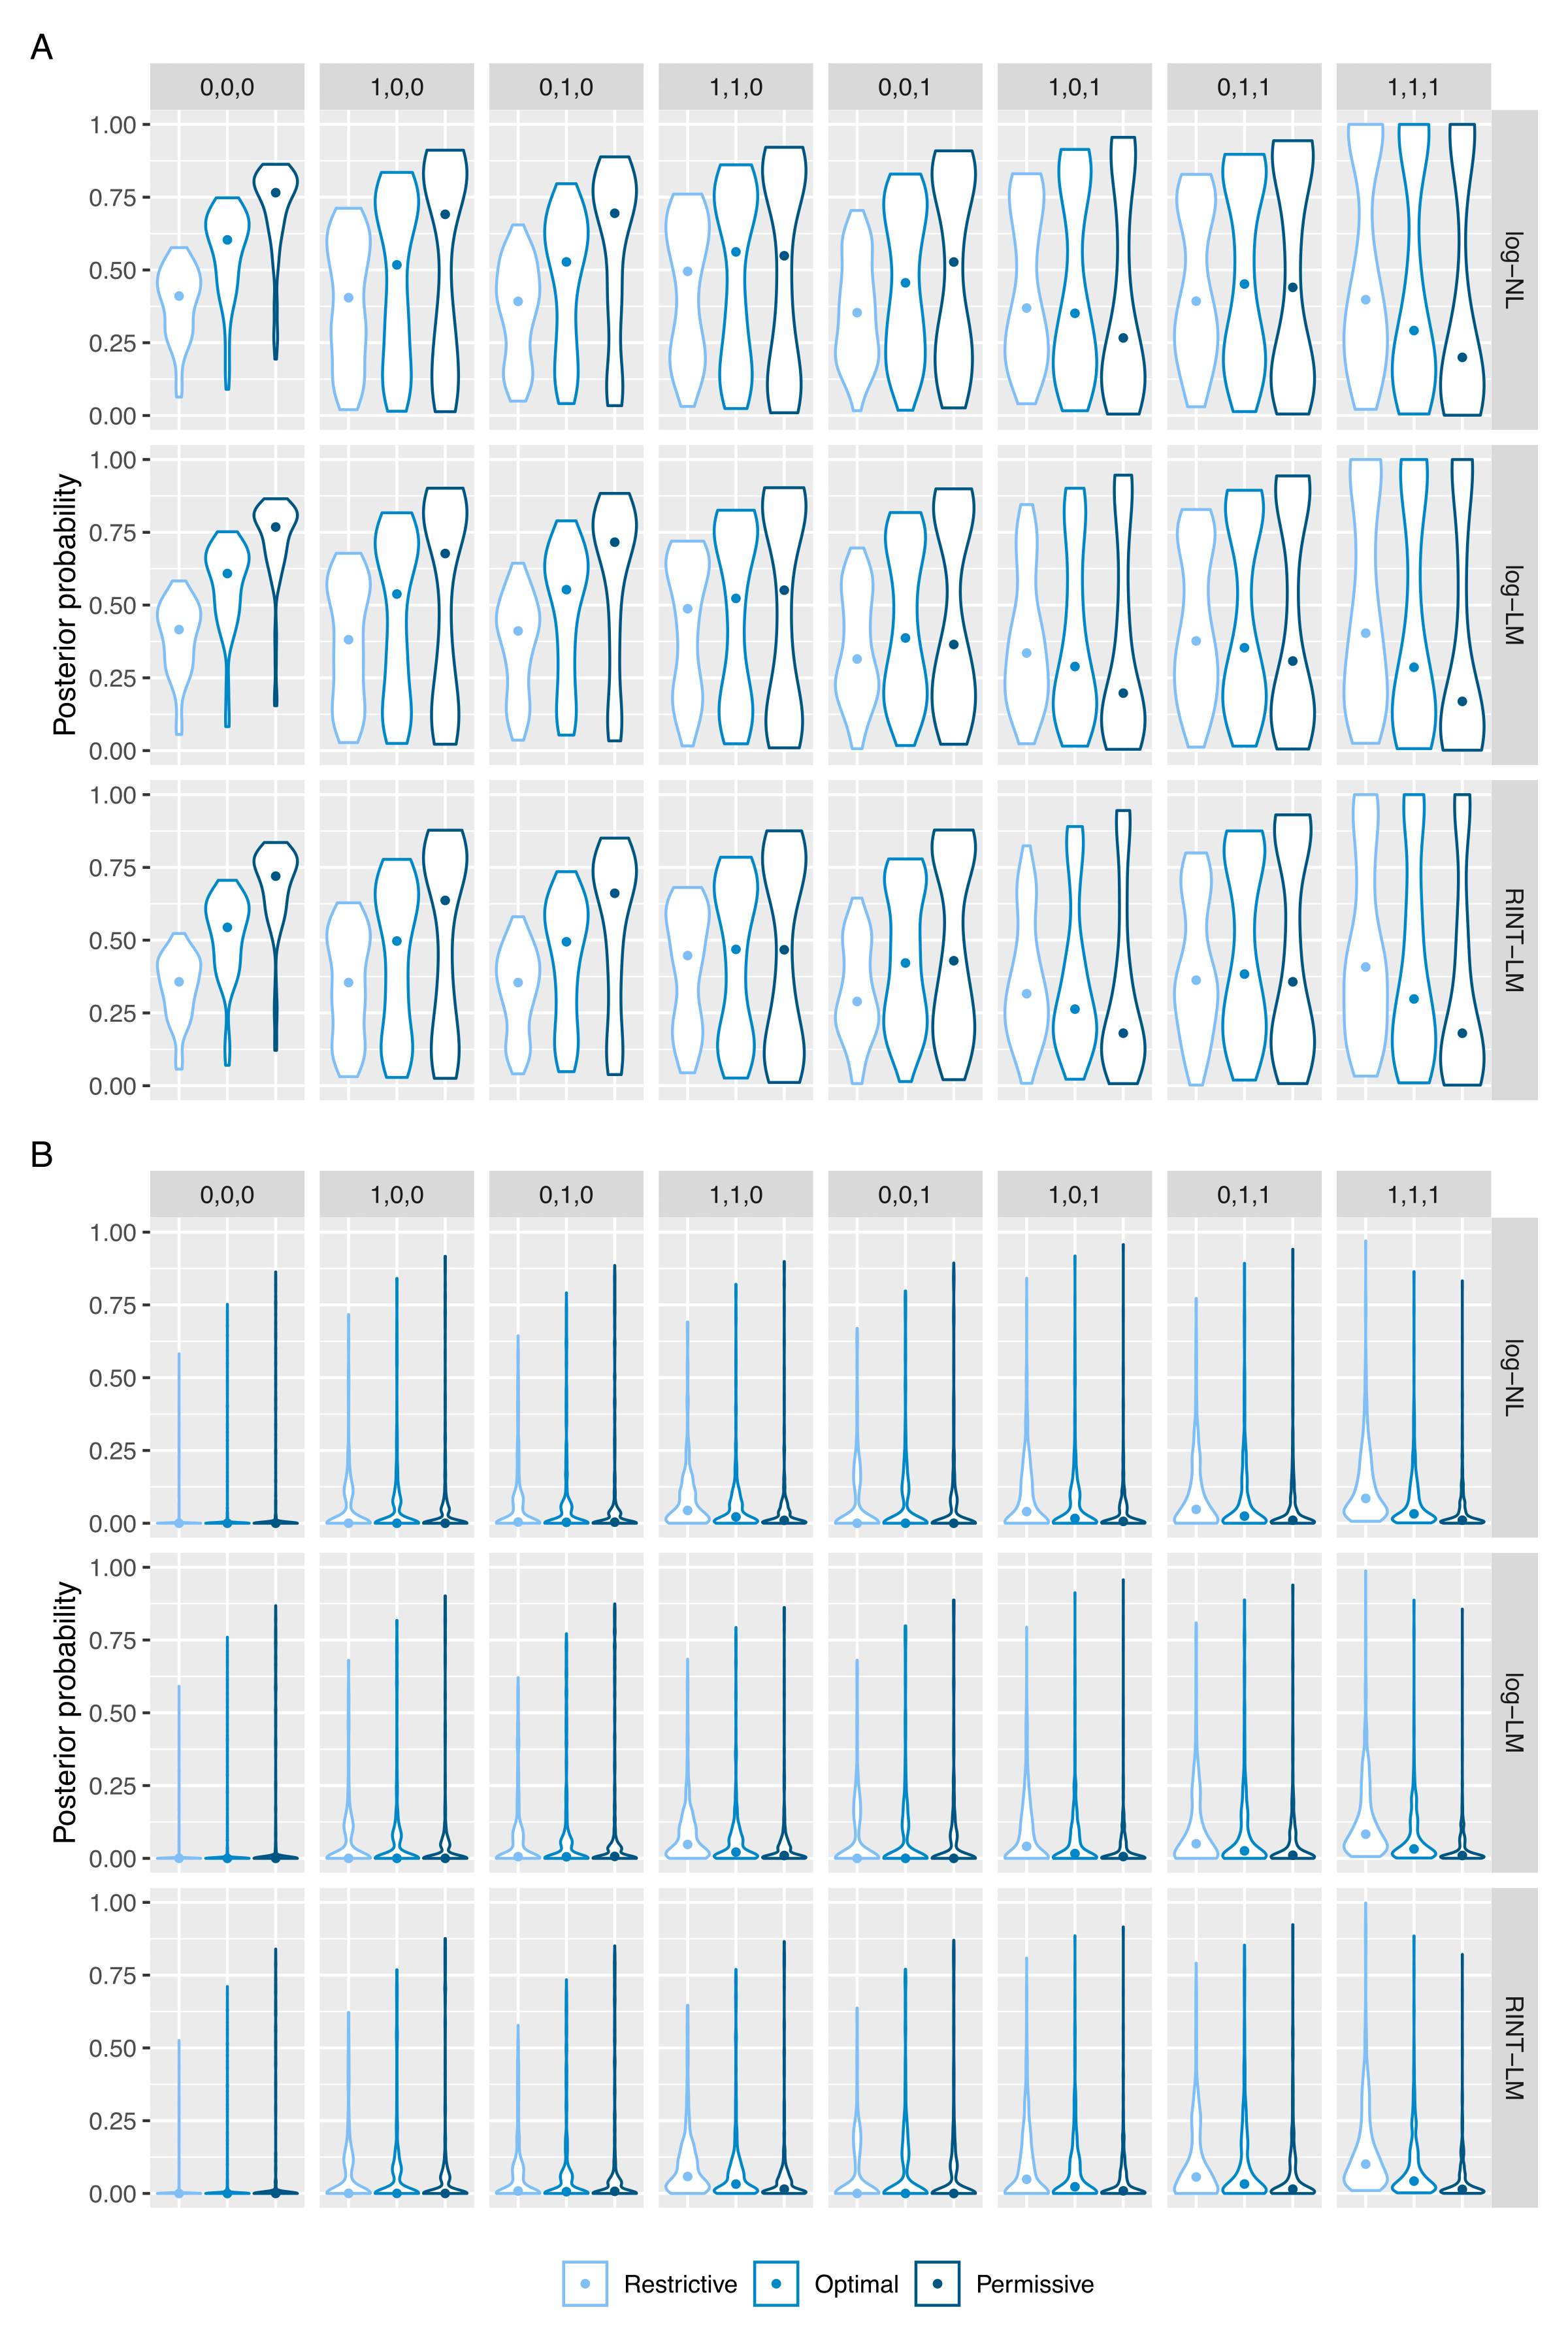
\includegraphics[width=0.75\textwidth]{png/sim_vln_effect_mcmc_bs_ranef_ranef.png}
\end{center}  
\caption{
  {\bf
    S13.4 Fig.
    Assessing the impact of the effect prior on the posterior probability of the correct and incorrect models from analyses with donor random effect in both data generation and model fitting using MCMC and bridge sampling.}
The same as in \sfigppeffectone but in scenario 4, which is described in the legend to \sfigroccmcmc.
}
\label{s-fig:sim-effect-mcmc-ranef-ranef}
\end{figure}

\begin{figure}[!ht]
\begin{center}
  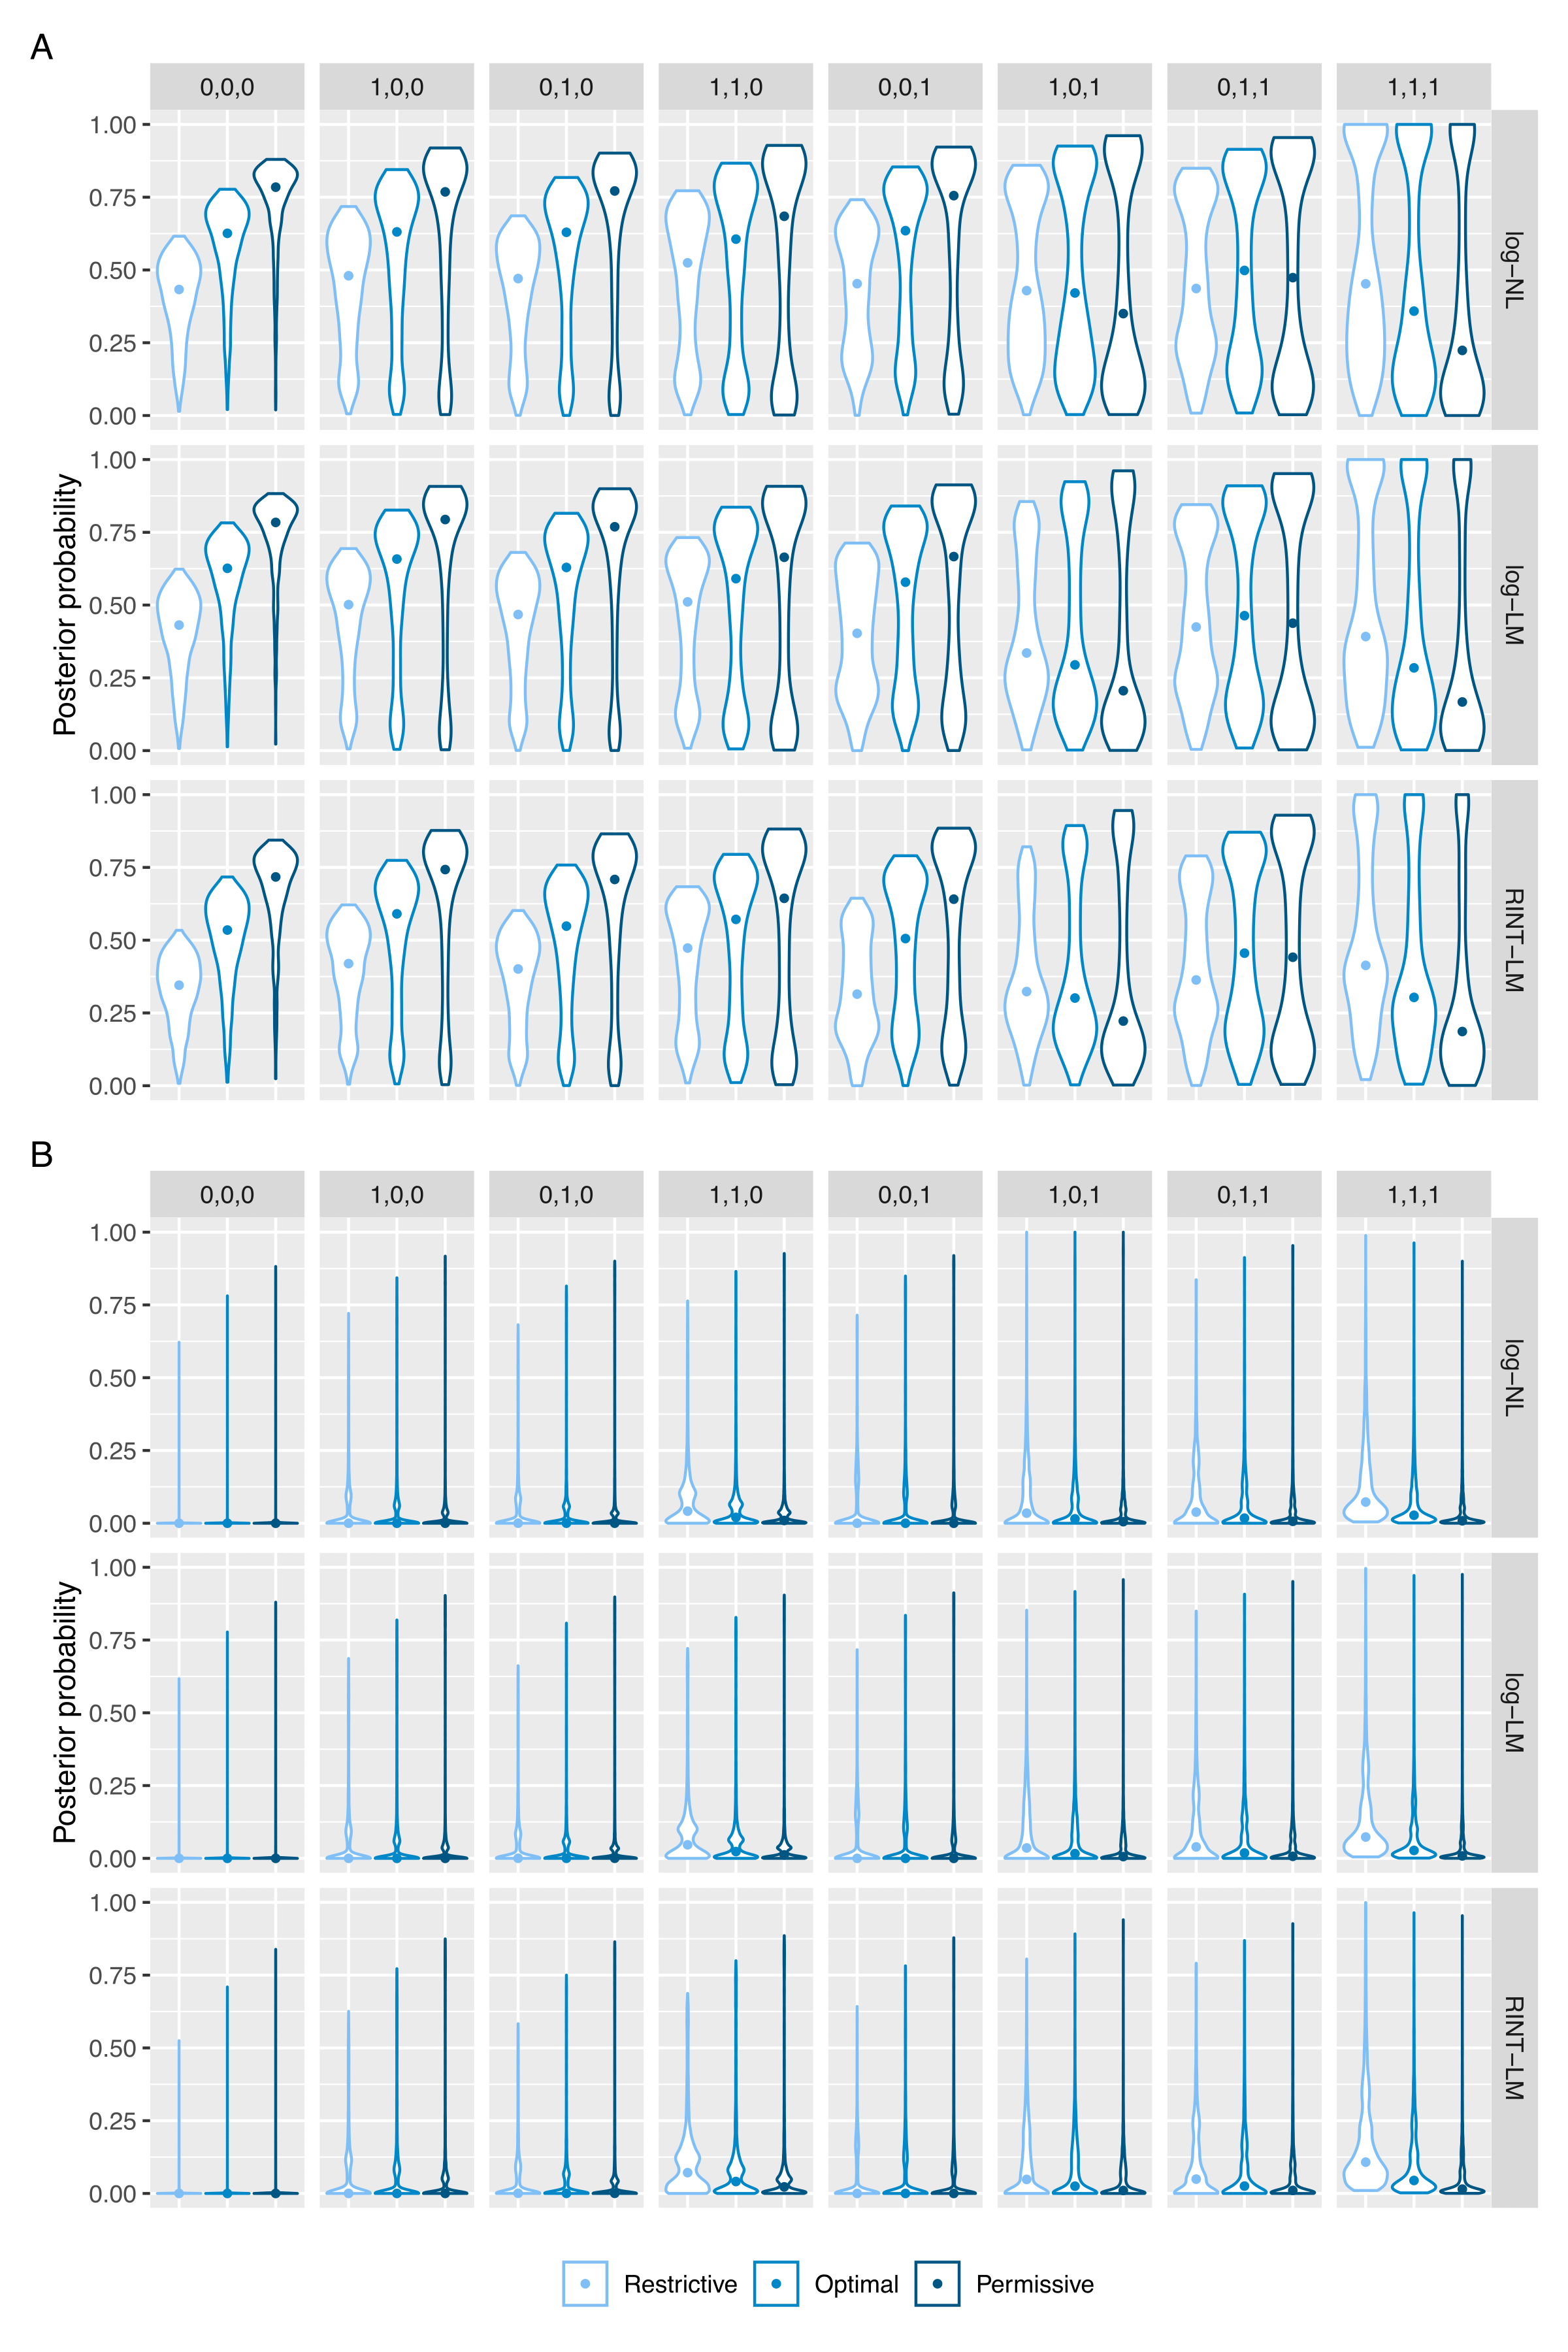
\includegraphics[width=0.75\textwidth]{png/sim_vln_effect_map_lap_noranef_noranef.png}
\end{center}  
\caption{
  {\bf
    S13.5 Fig.
    Assessing the impact of the effect prior on the posterior probability of the correct and incorrect models from analyses without random effect using MAP estimation and Laplace approximation.}
The same as in \sfigppeffectone but for MAP estimation and Laplace approximation.
}
\label{s-fig:sim-effect-map-noranef-noranef}
\end{figure}

\begin{figure}[!ht]
\begin{center}
  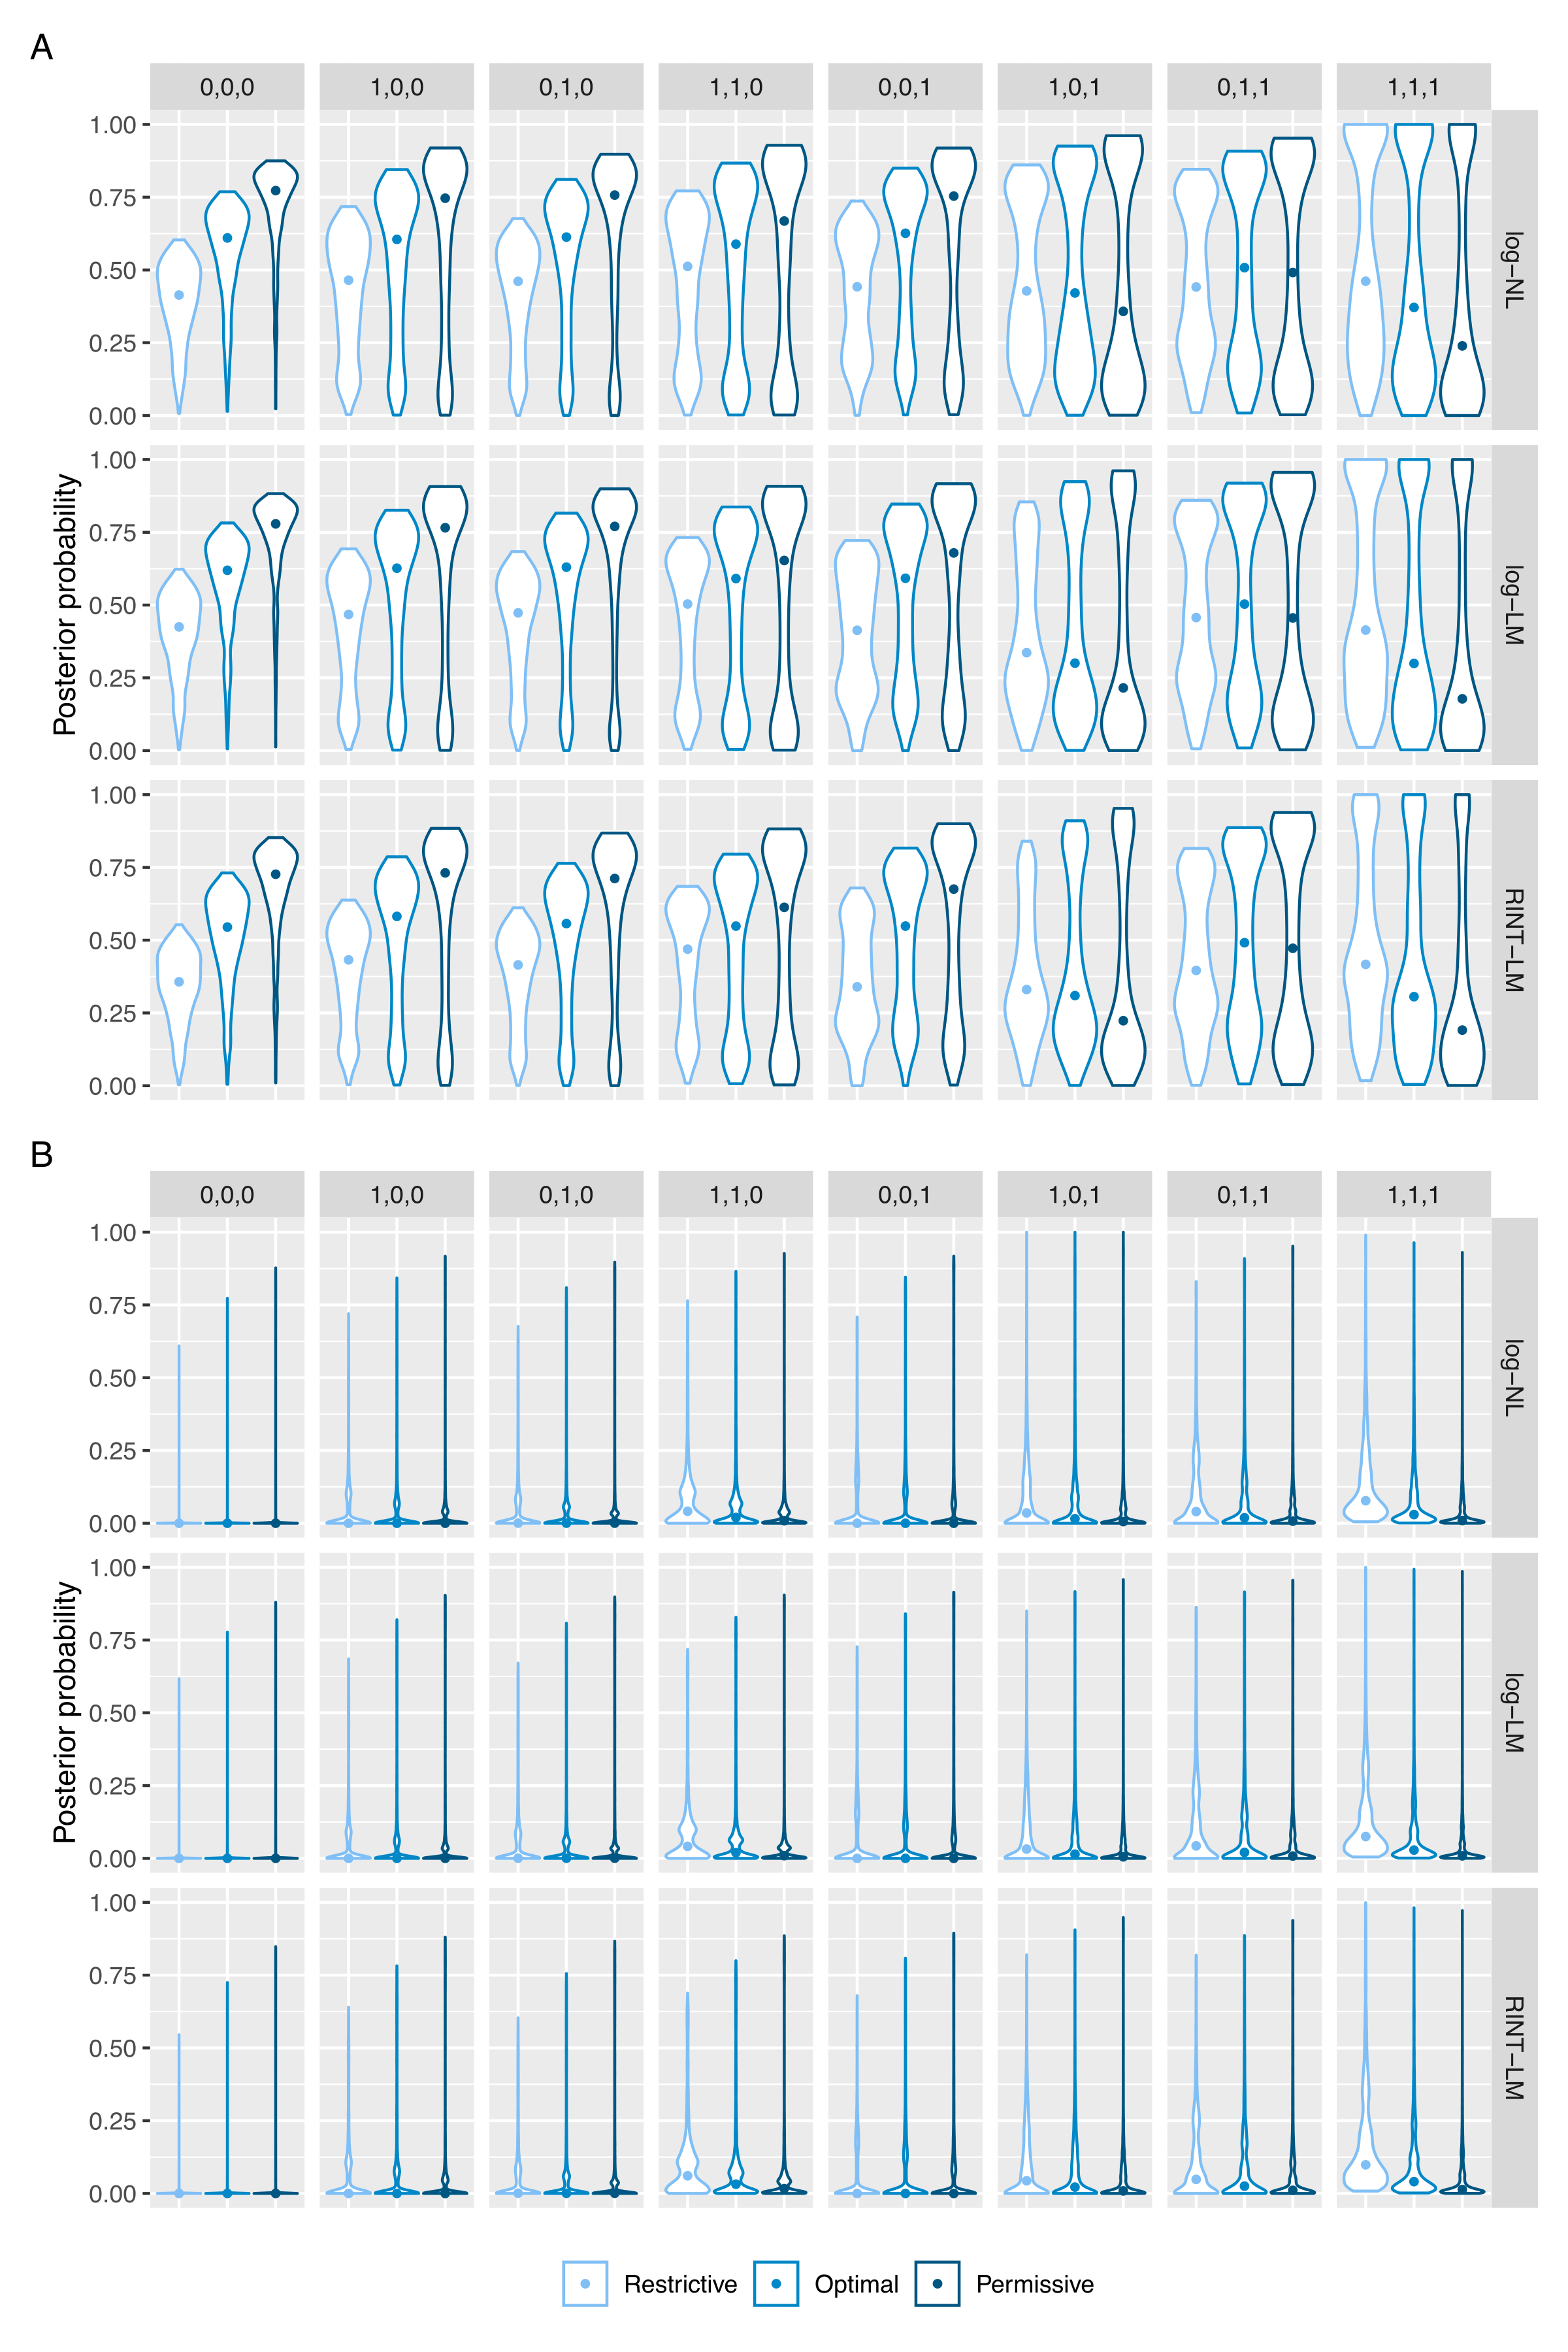
\includegraphics[width=0.75\textwidth]{png/sim_vln_effect_map_lap_noranef_ranef.png}
\end{center}  
\caption{
  {\bf
    S13.6 Fig.
    Assessing the impact of the effect prior on the posterior probability of the correct and incorrect models from analyses with donor random effect in model fitting but not in data generation using MAP estimation and Laplace approximation.}
The same as in \sfigppeffecttwo but for MAP estimation and Laplace approximation.
}
\label{s-fig:sim-effect-map-noranef-ranef}
\end{figure}

\begin{figure}[!ht]
\begin{center}
  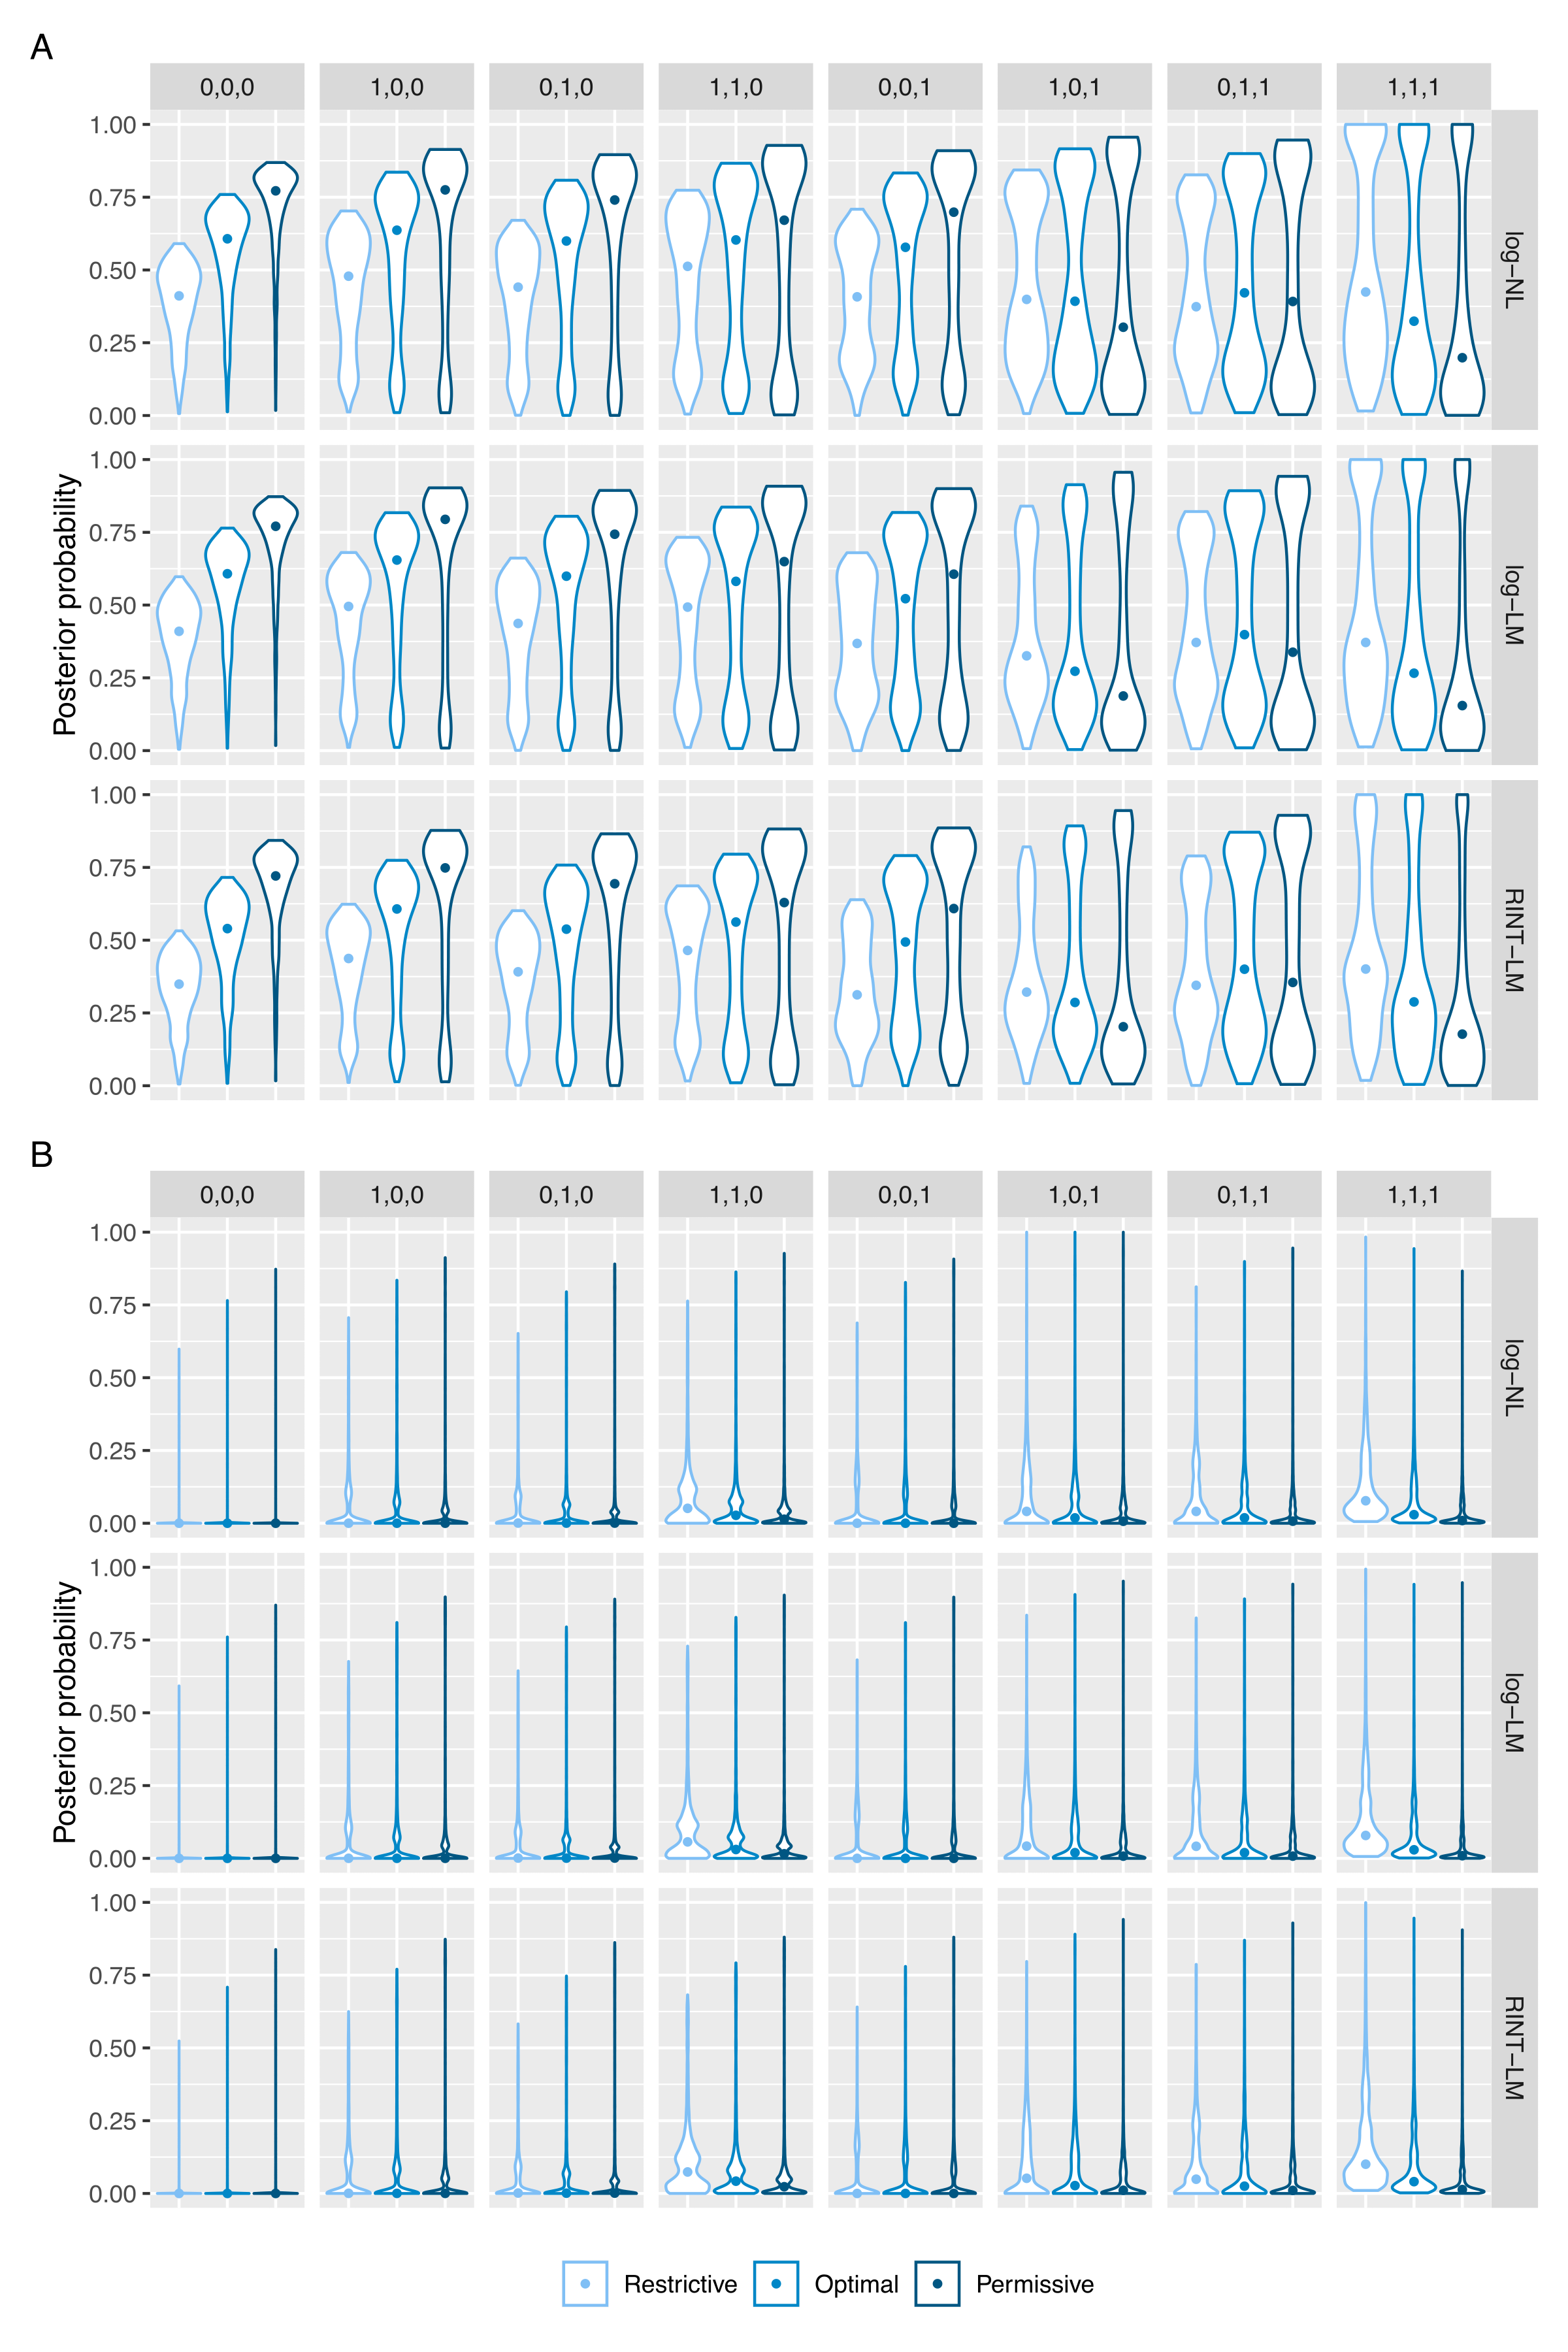
\includegraphics[width=0.75\textwidth]{png/sim_vln_effect_map_lap_ranef_noranef.png}
\end{center}  
\caption{
  {\bf
    S13.7 Fig.
    Assessing the impact of the effect prior on the posterior probability of the correct and incorrect models from analyses with donor random effect in data generation but not in model fitting using MAP estimation and Laplace approximation.}
The same as in \sfigppeffectthree but for MAP estimation and Laplace approximation.
}
\label{s-fig:sim-effect-map-ranef-noranef}
\end{figure}

\begin{figure}[!ht]
\begin{center}
  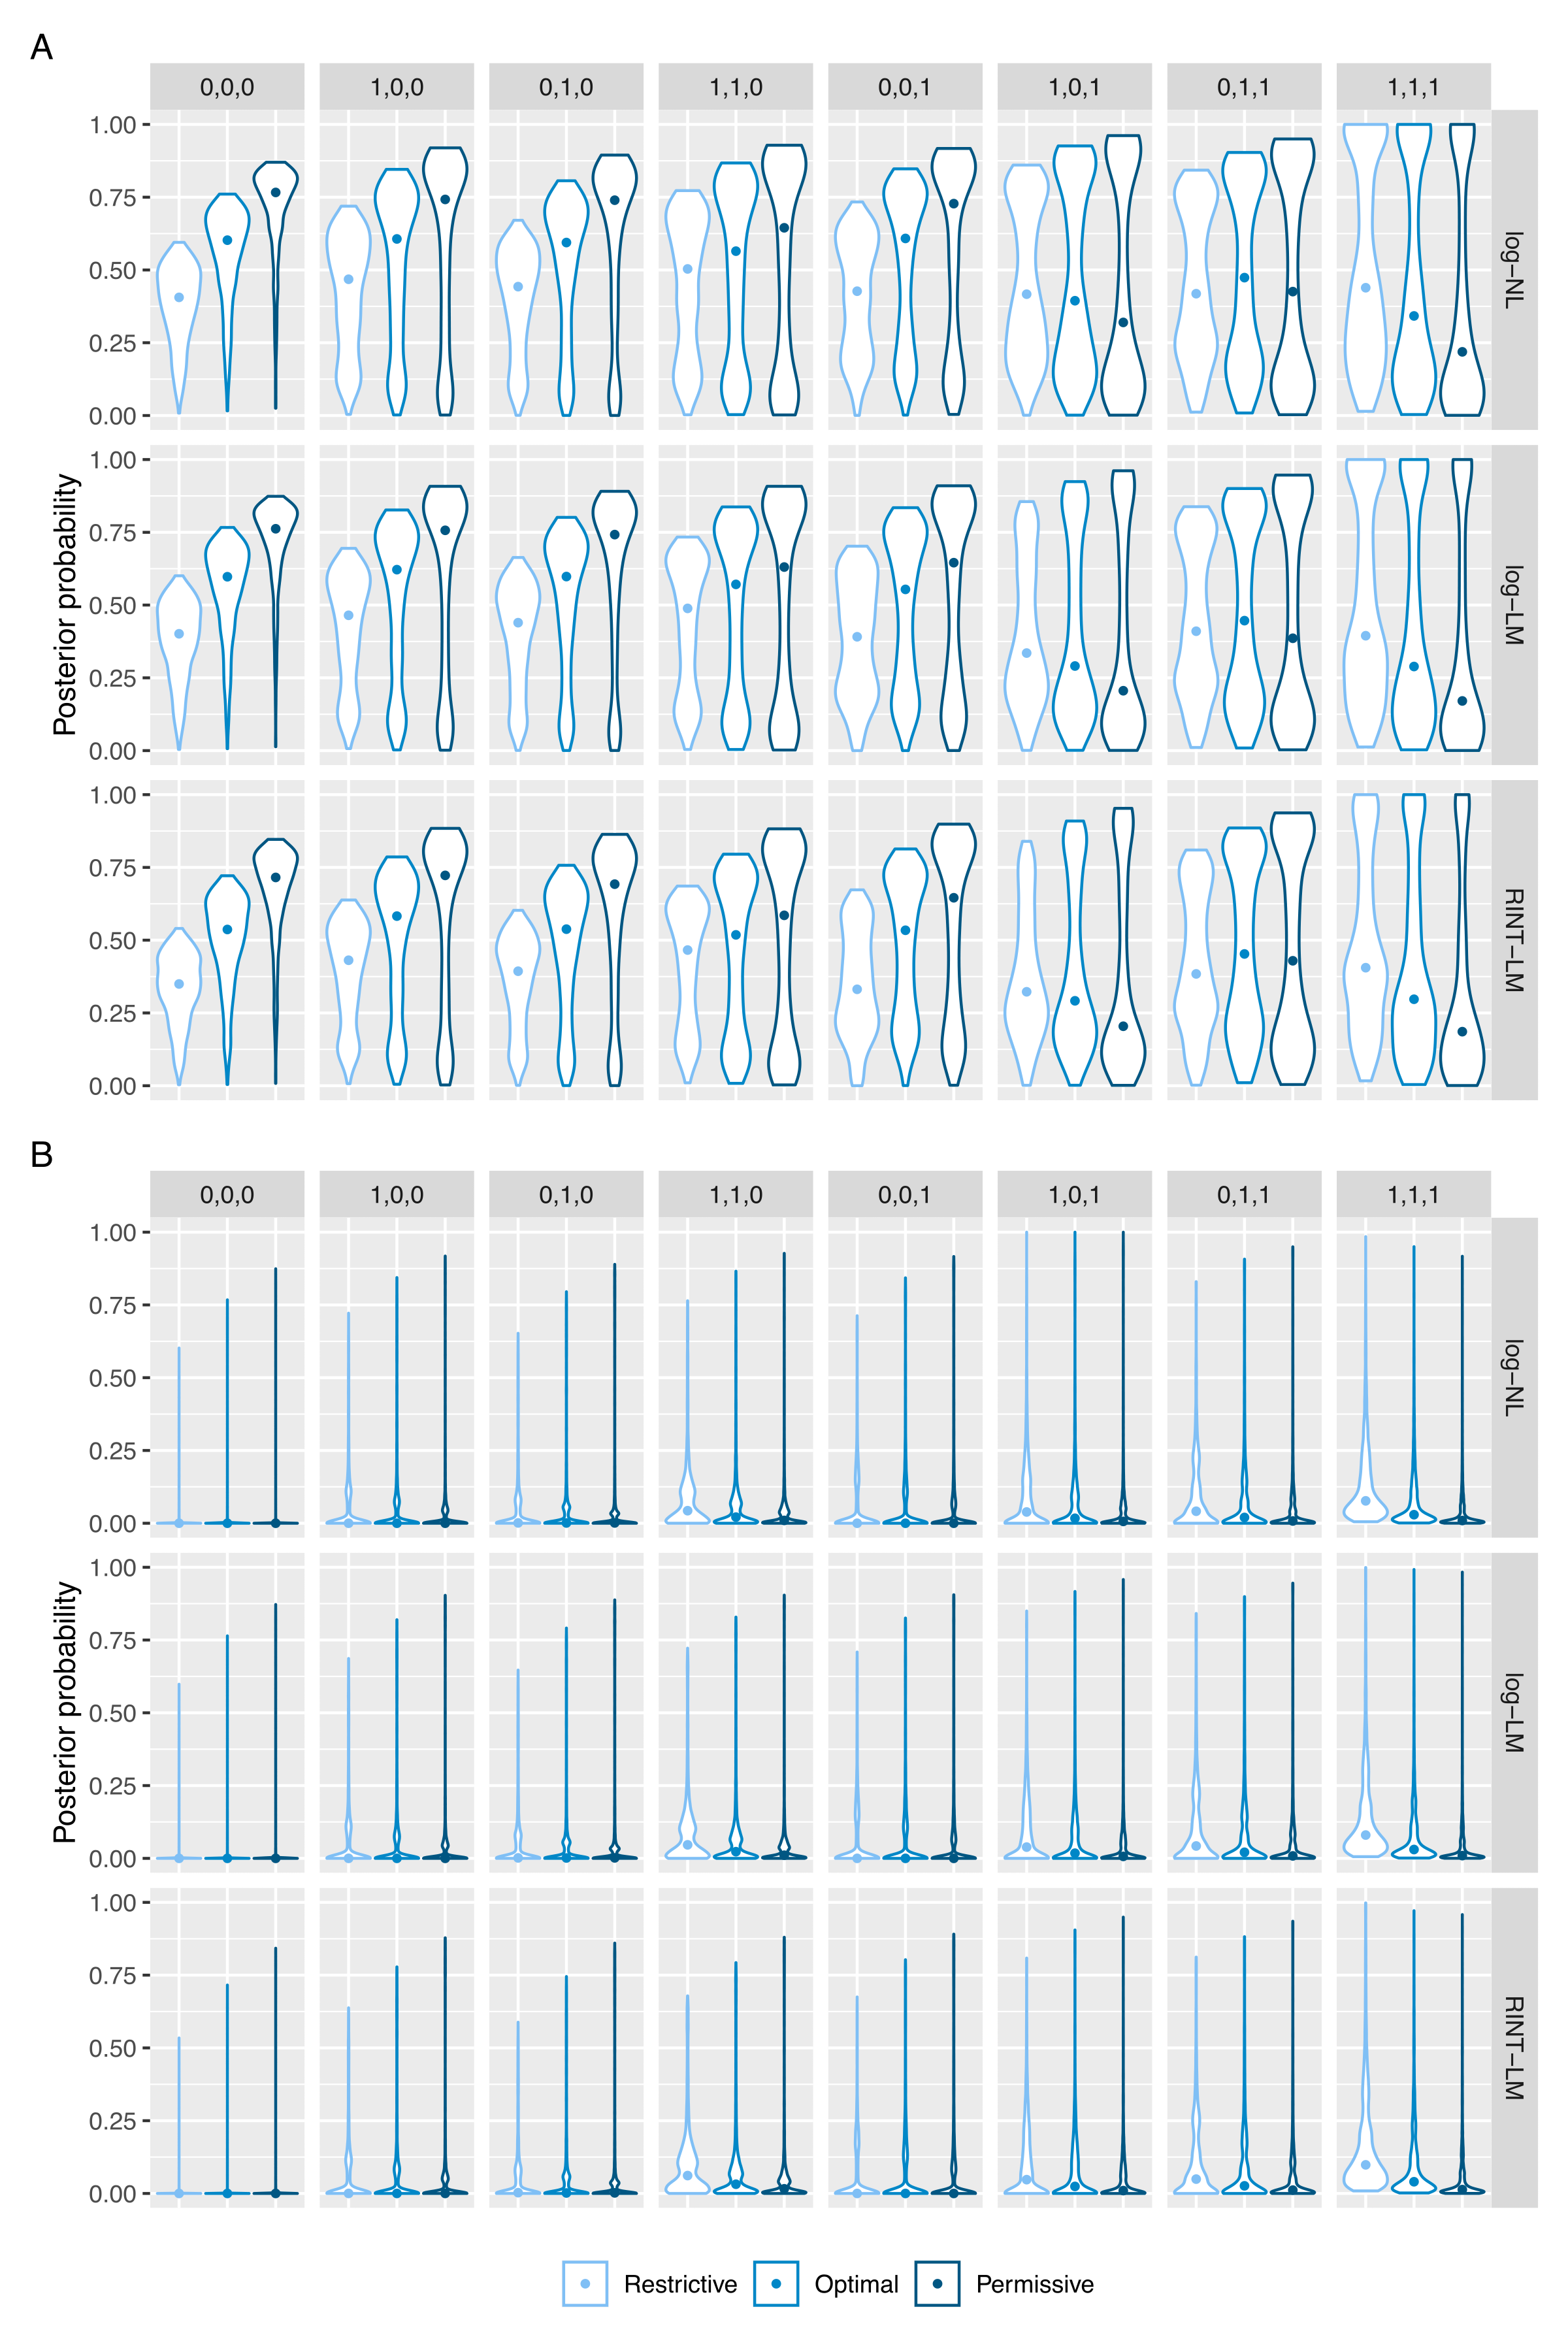
\includegraphics[width=0.75\textwidth]{png/sim_vln_effect_map_lap_ranef_ranef.png}
\end{center}  
\caption{
  {\bf
    S13.8 Fig.
    Assessing the impact of the effect prior on the posterior probability of the correct and incorrect models from analyses with donor random effect in both data generation and model fitting using MAP estimation and Laplace approximation.}
The same as in \sfigppeffectfour but for MAP estimation and Laplace approximation.
}
\label{s-fig:sim-effect-map-ranef-ranef}
\end{figure}

\begin{figure}[!ht]
\begin{center}
  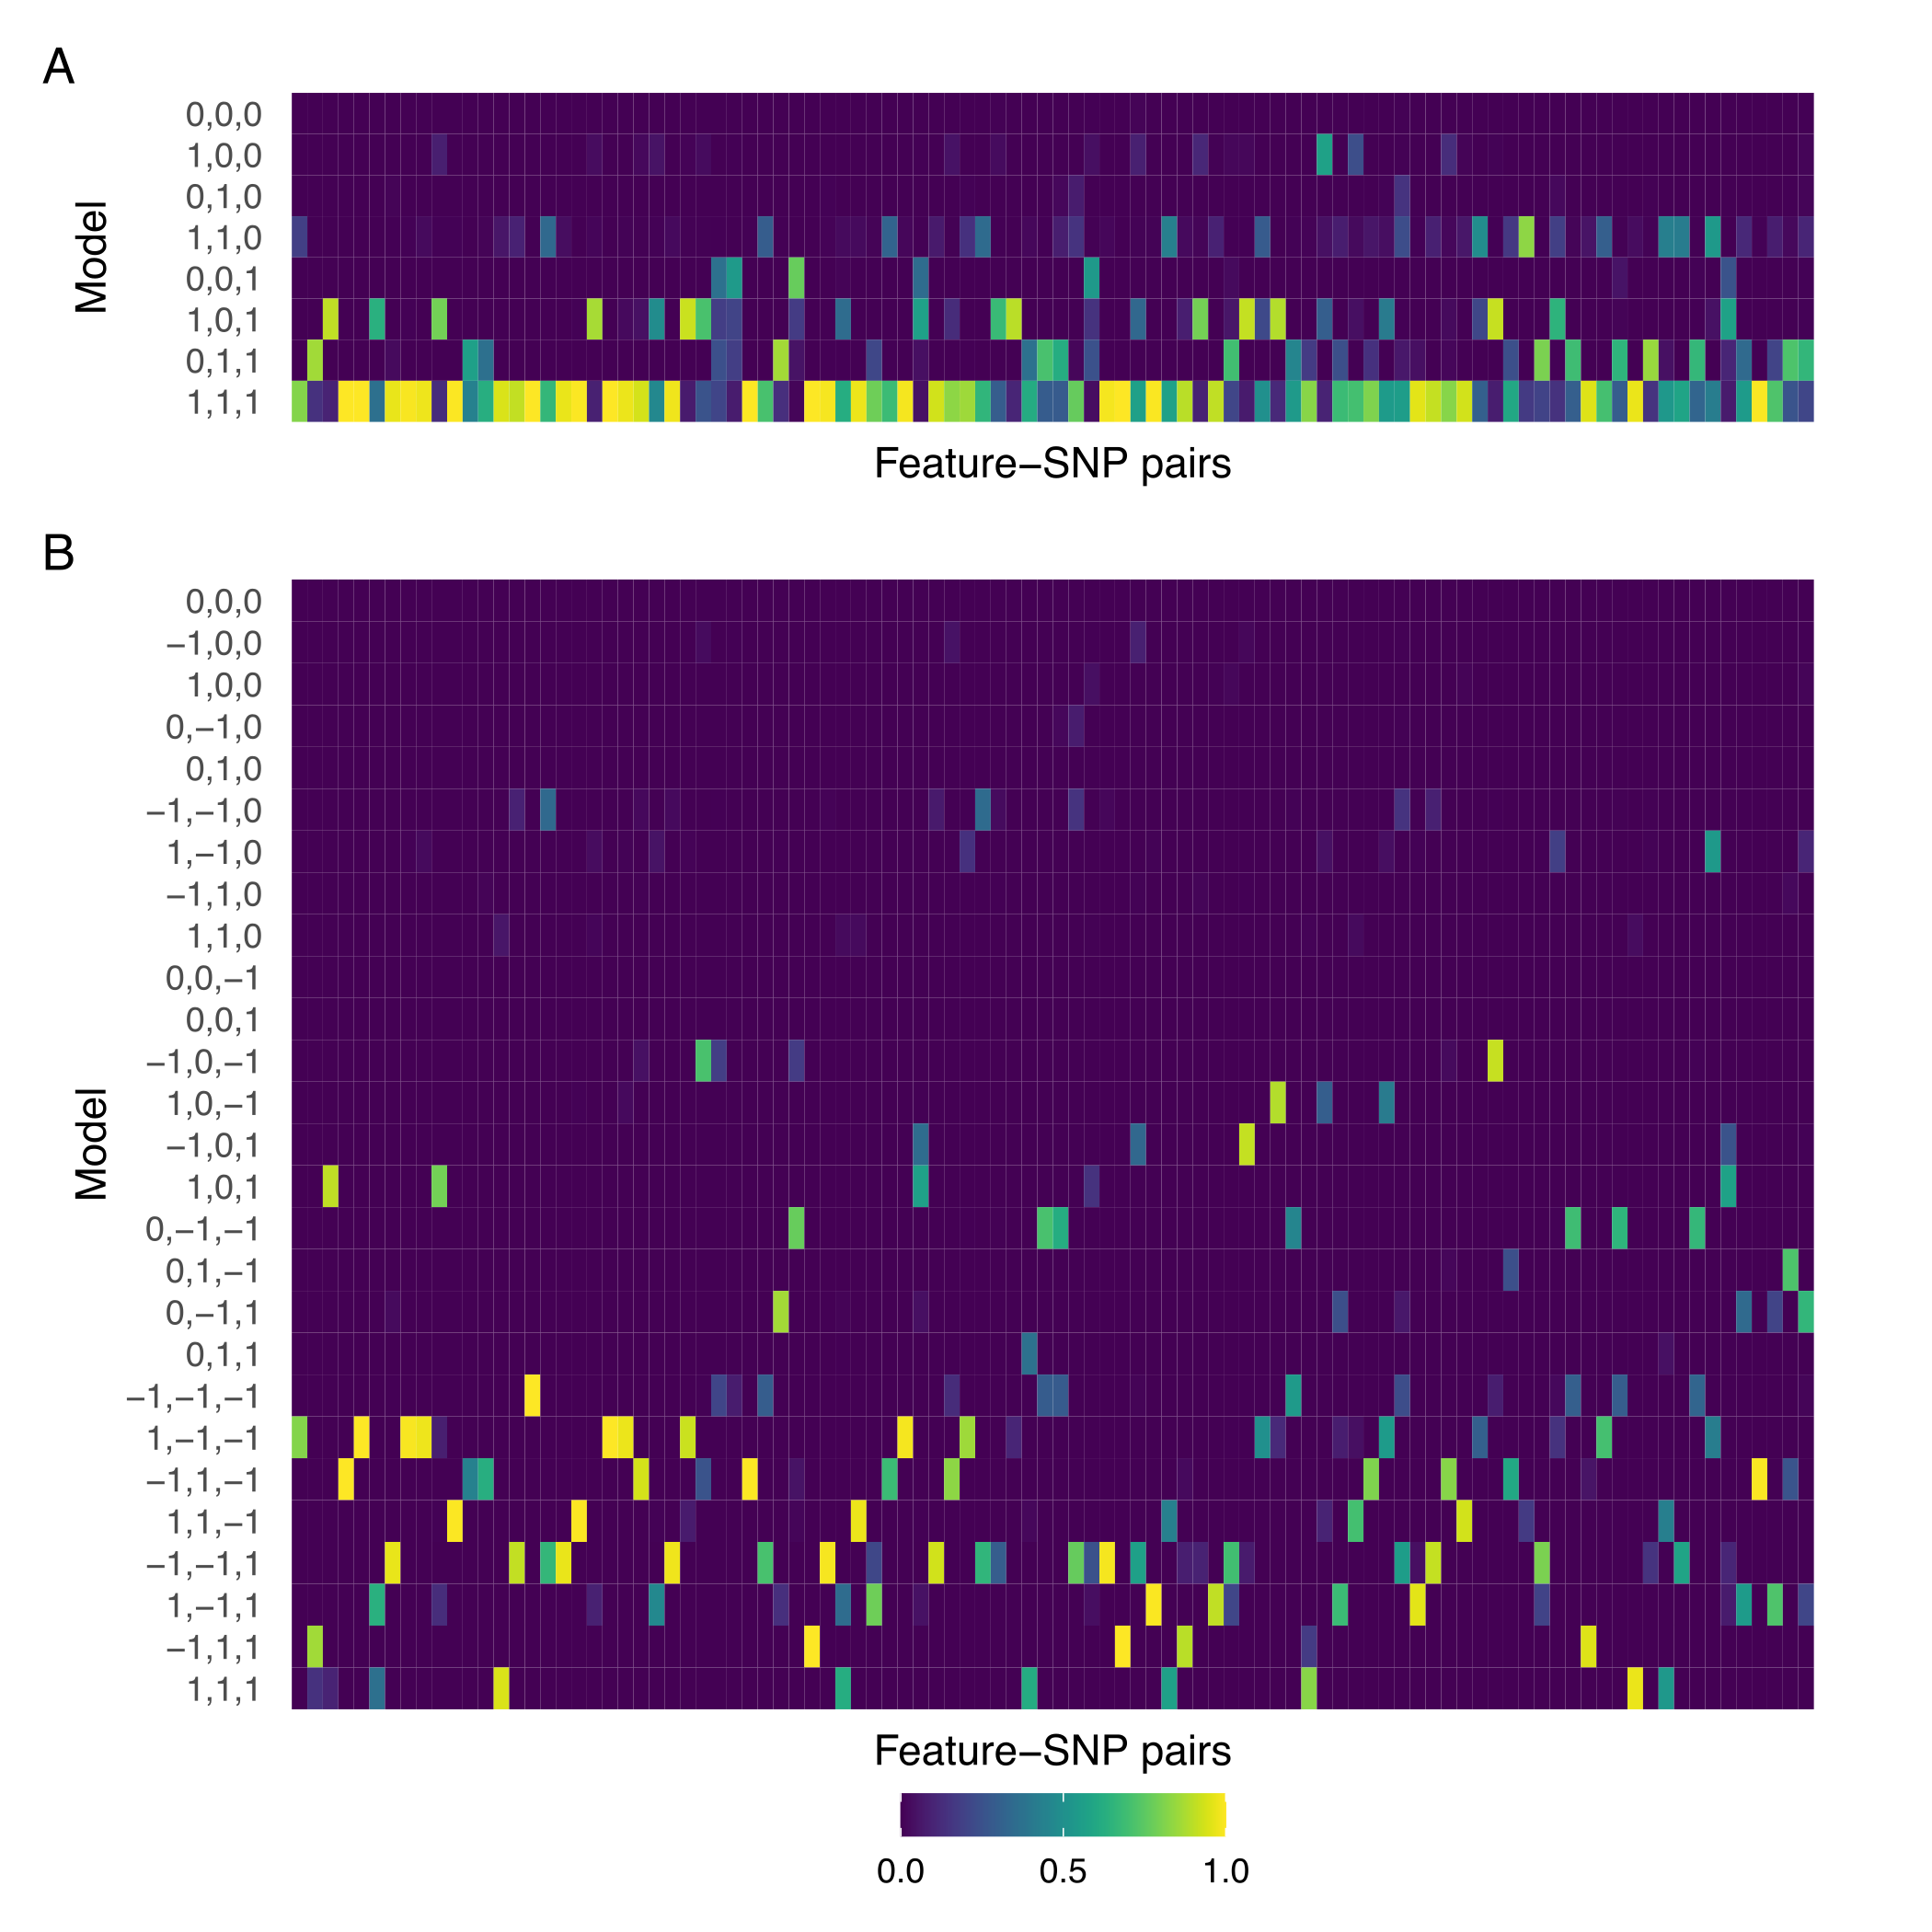
\includegraphics[width=0.8\textwidth]{png/wntrna_hm.png}
\end{center}  
\caption{
  {\bf
    S14 Fig.
    Posterior probability of the models with and without accounting for the sign of effect size for the response eQTL data in hNPCs.}
The heatmaps show the posterior probability of the eight models for the 98 response eQTLs, which represent gene-SNP pairs with significant \GxT interactions (\textbf{A}), as well as that of the 27 models accounting for the sign of effect size (\textbf{B}).
The rows and columns represent the models and gene-SNP pairs, respectively. The gene-SNP pairs are ordered by $P$ values for significant \GxT interactions. The leftmost column corresponds to the smallest $P$ value.
}
\label{s-fig:wntrna-sign}
\end{figure}

\begin{figure}[!ht]
\begin{center}
  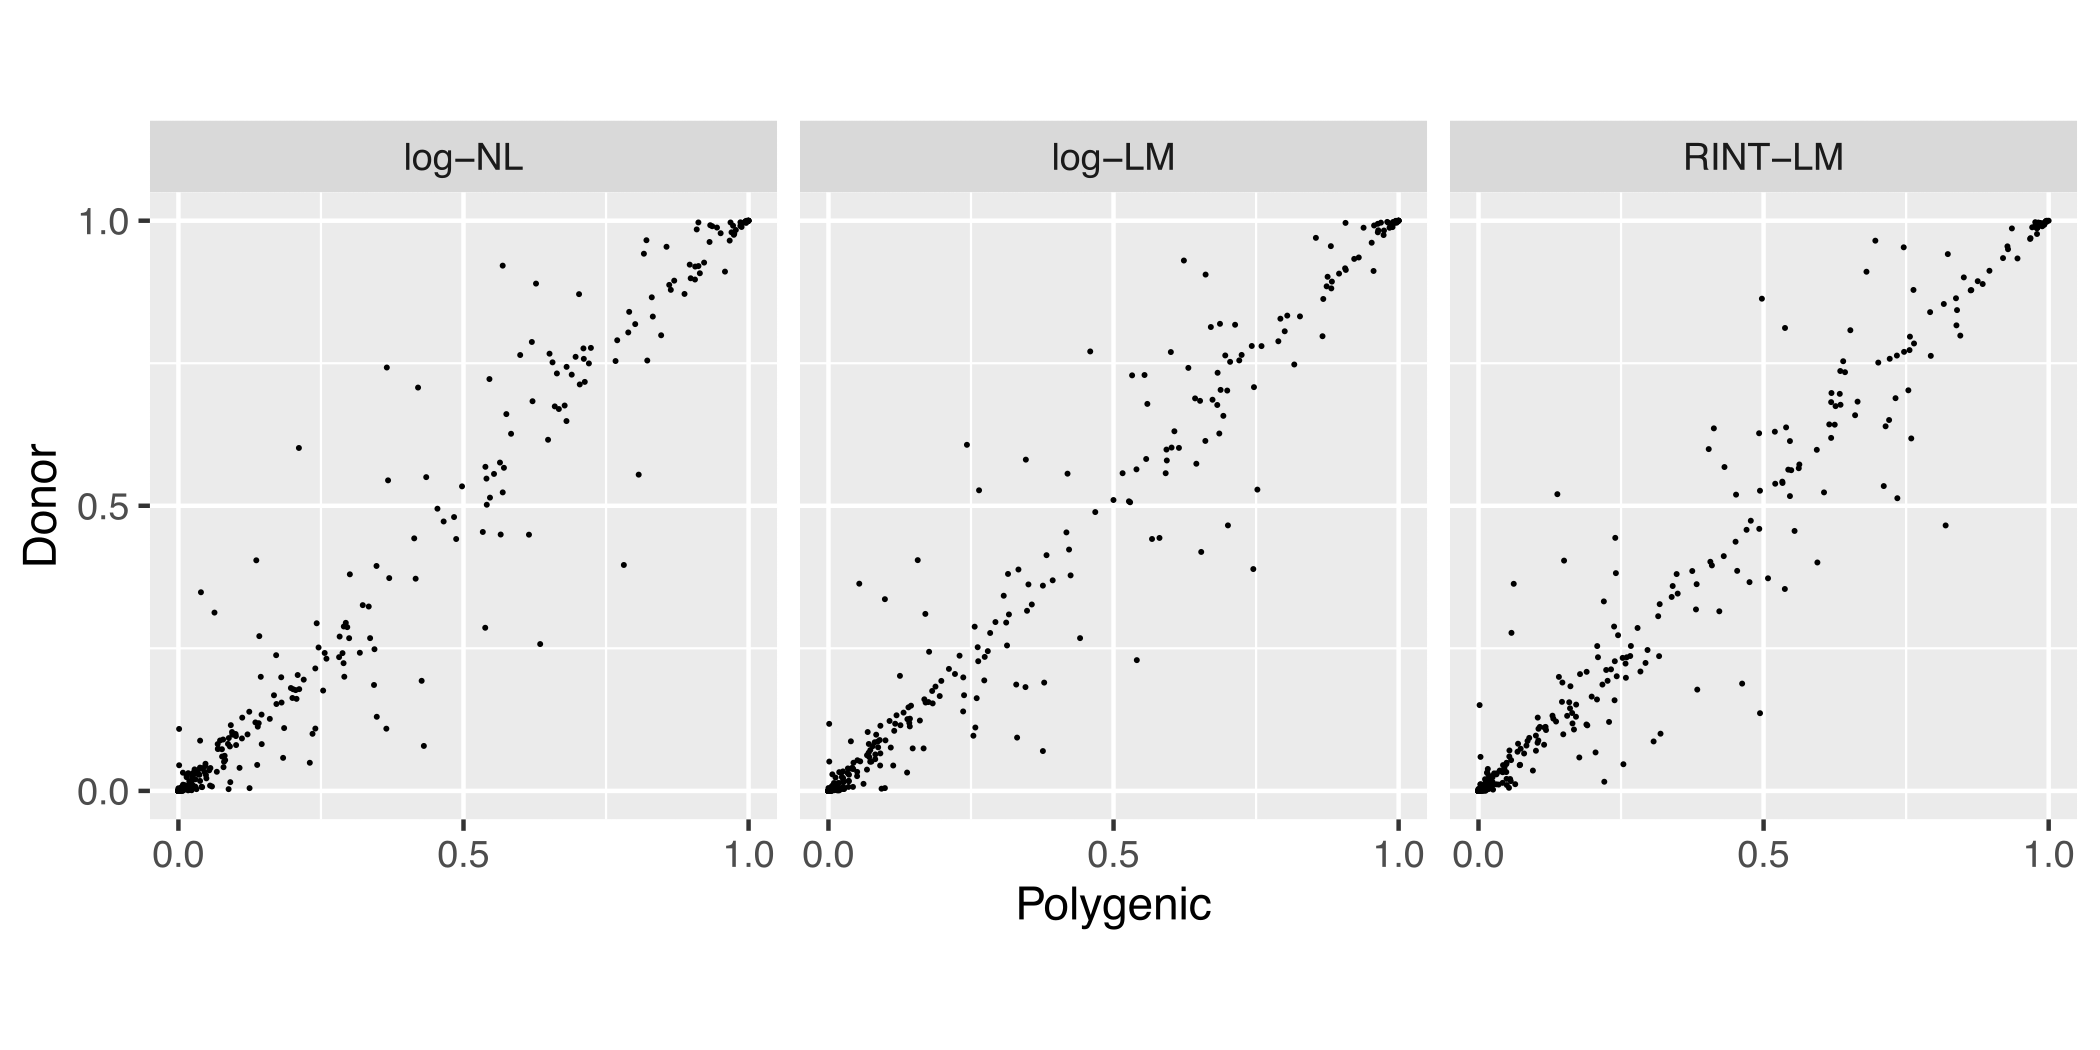
\includegraphics[width=0.8\textwidth]{png/wntrna_compare_pp.png}
\end{center}  
\caption{
  {\bf
    S15 Fig.
    Comparison of posterior probability between results with donor random effect and those with polygenic random effect for response eQTLs.}
Scatter plots comparing results obtained by BMS with polygenic (kinship) random effect and those with donor random effect for $\log$-NL, $\log$-LM, and RINT-LM. Each point represents the posterior probability of a mode for a feature-SNP pair. The values are compared across eight models and 98 feature-SNP pairs (i.e., 784 combinations).
}
\label{s-fig:wntrna-compare-pp}
\end{figure}

\begin{figure}[!ht]
\begin{center}
  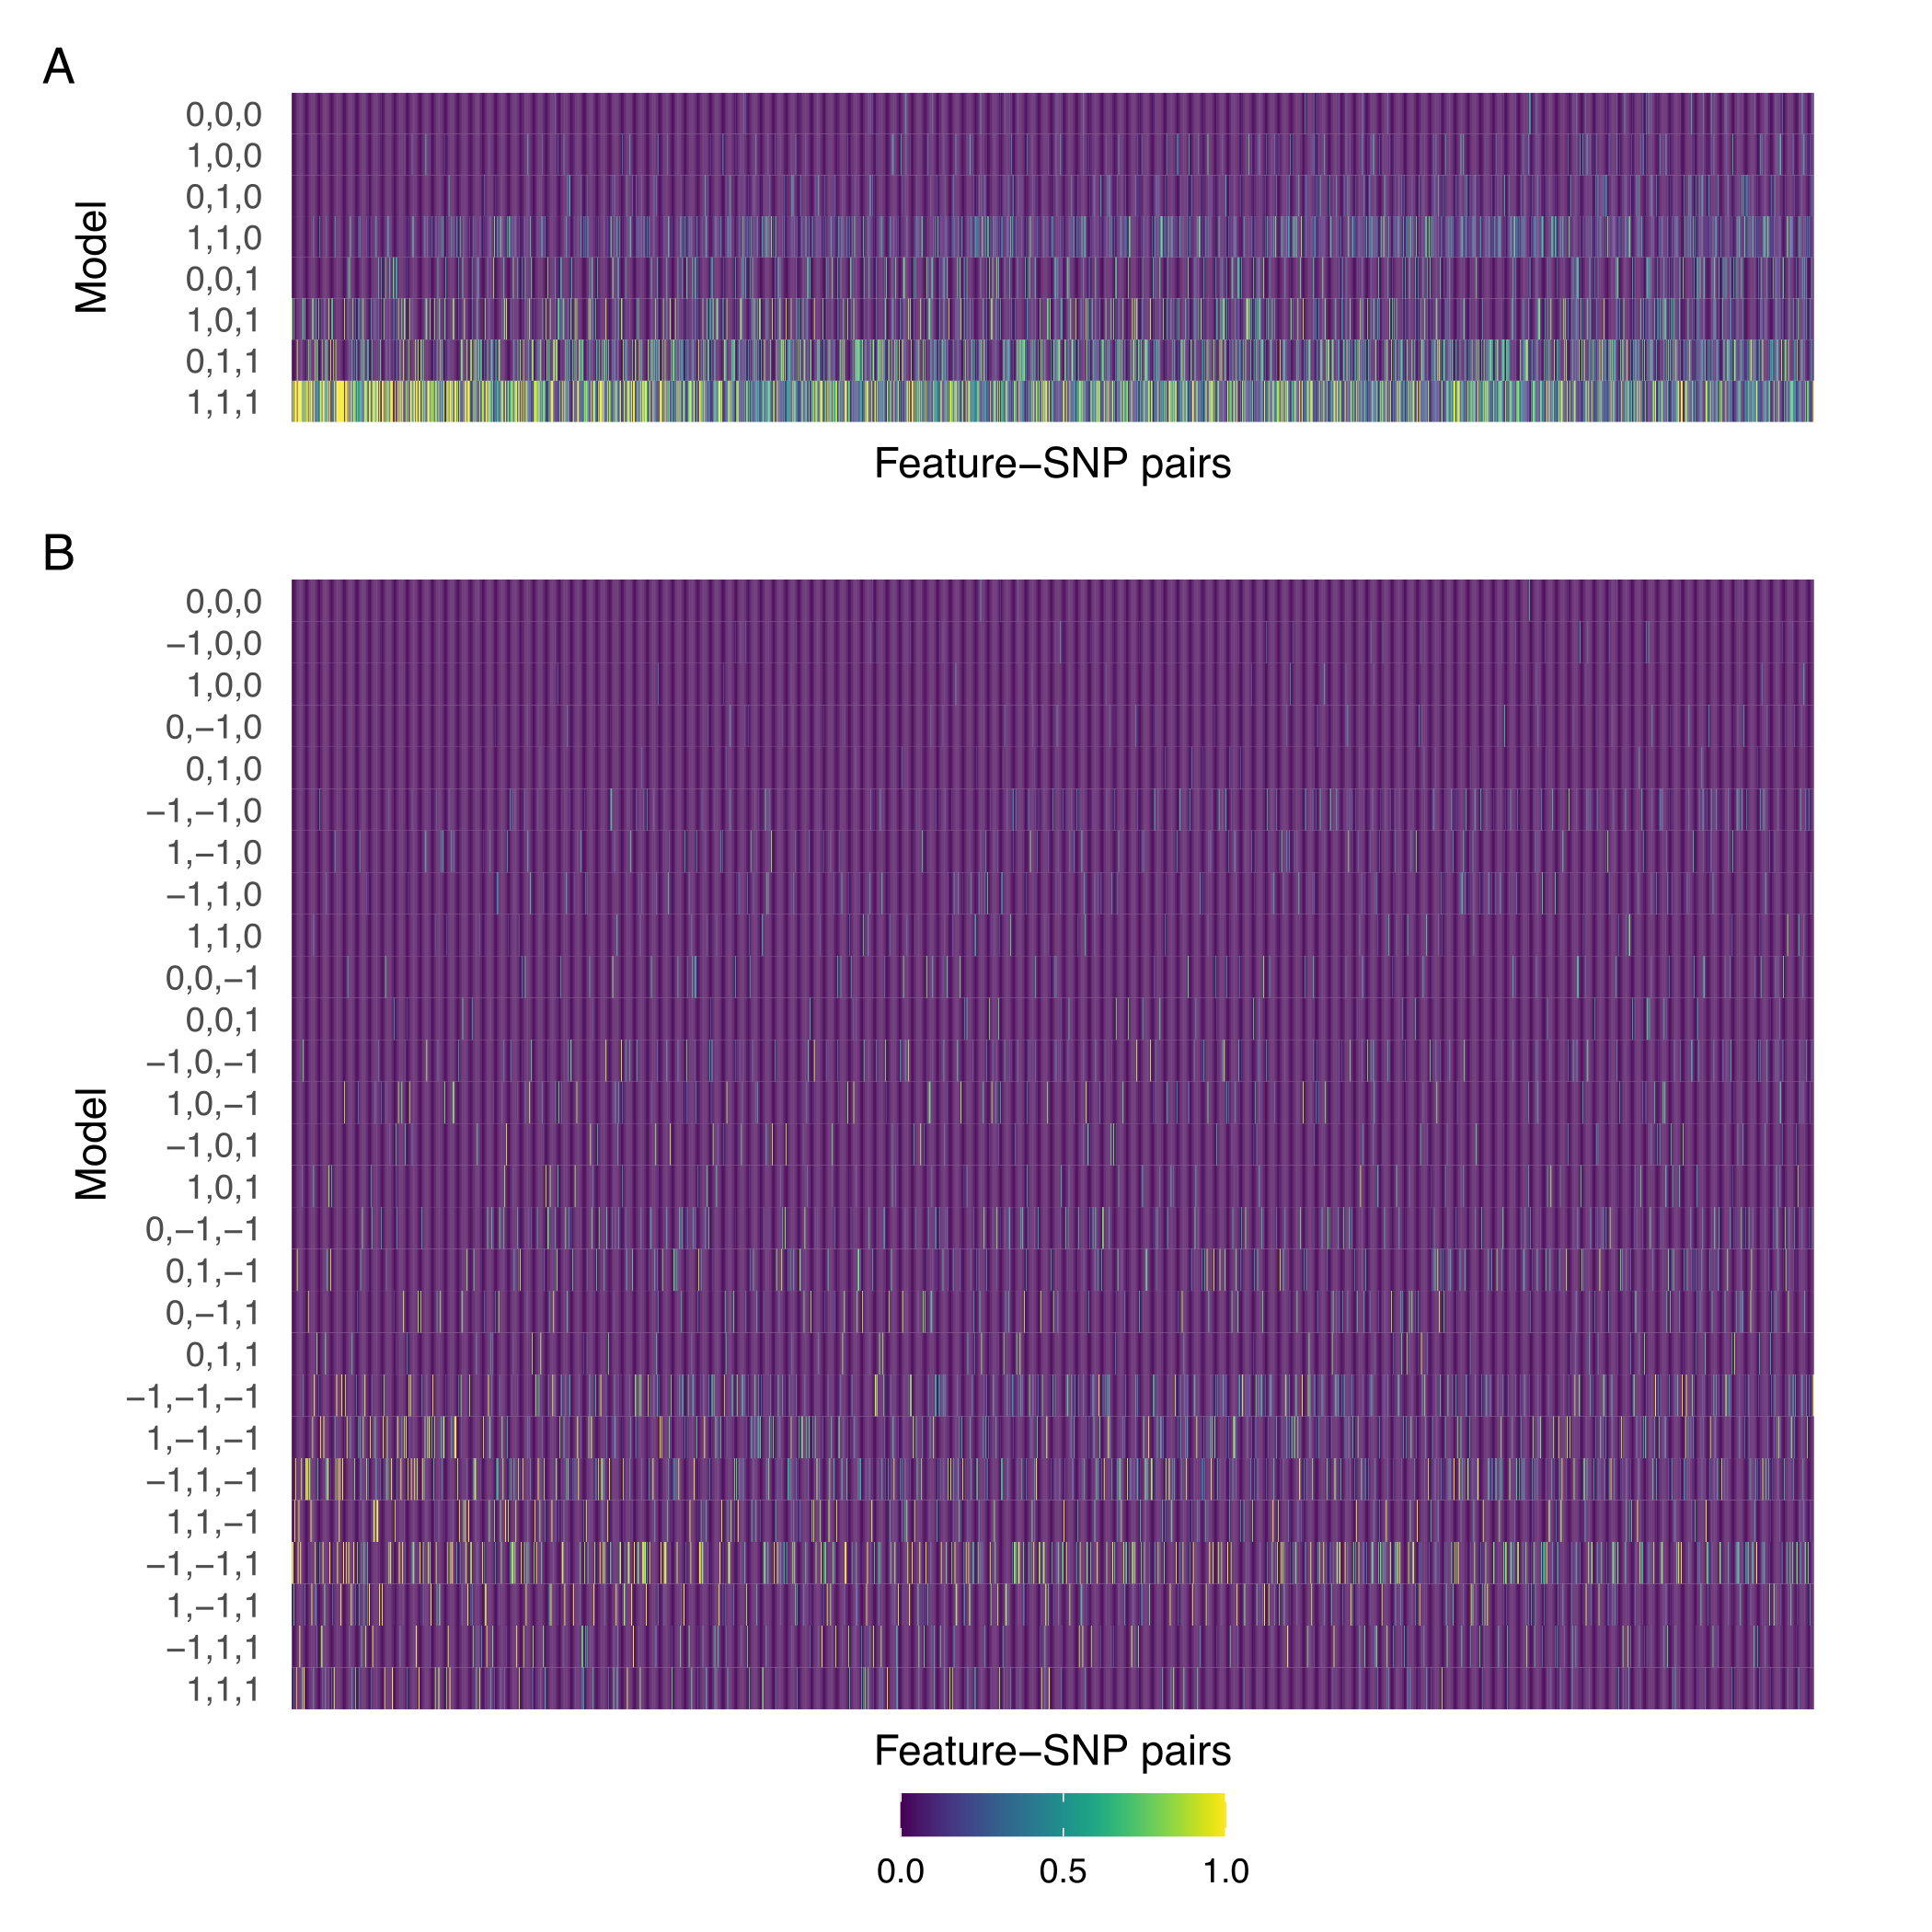
\includegraphics[width=1\textwidth]{png/wntatac_hm.png}
\end{center}  
\caption{
  {\bf
    S16 Fig.
    Posterior probability of the models with and without accounting for the sign of effect size for the response caQTL data in hNPCs.}
The same as in \sfigwntrnahm but for 1775 response caQTLs. 
}
\label{s-fig:wntatac-sign}
\end{figure}

\begin{figure}[!ht]
\begin{center}
  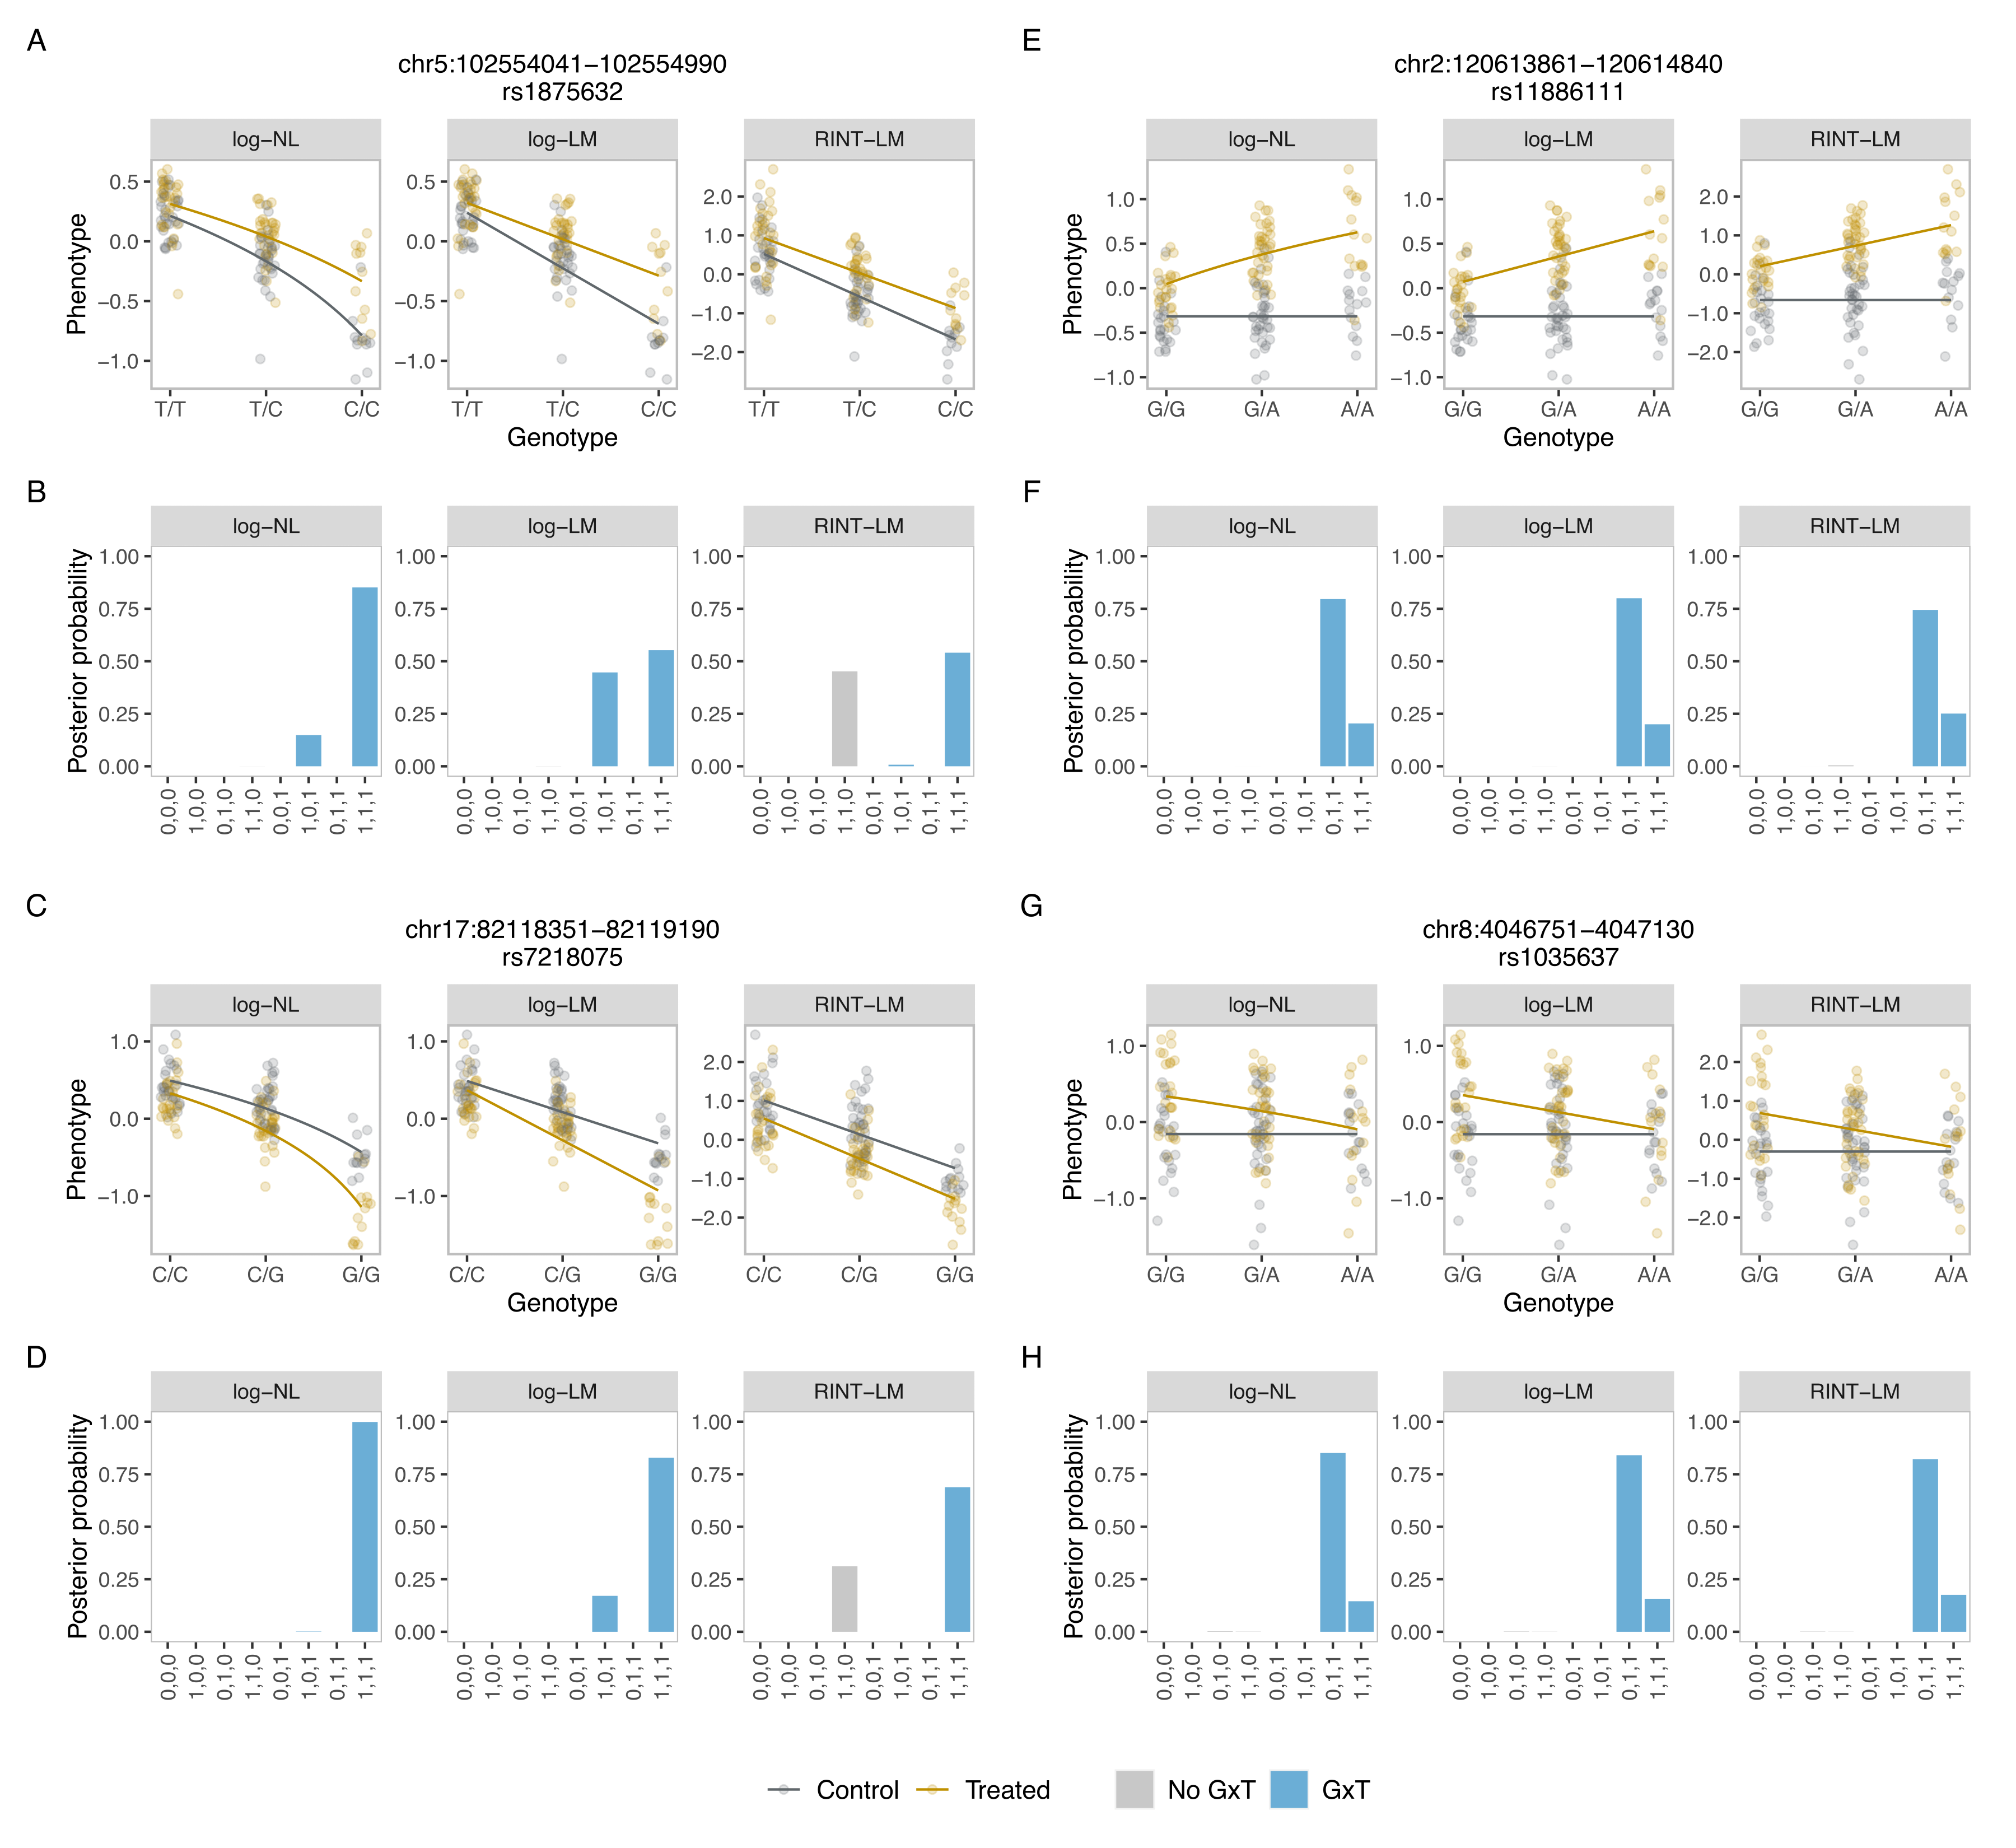
\includegraphics[width=1\textwidth]{png/wntatac_gp.png}
\end{center}  
\caption{
  {\bf
    S17 Fig.
    Representative BMS results for the response caQTL data in hNPCs.}
The same as in \figwntrnabms (see the main text) but for response caQTLs. 
}
\end{figure}
\label{s-fig:wntatac-gp}

\begin{figure}[!ht]
\begin{center}
  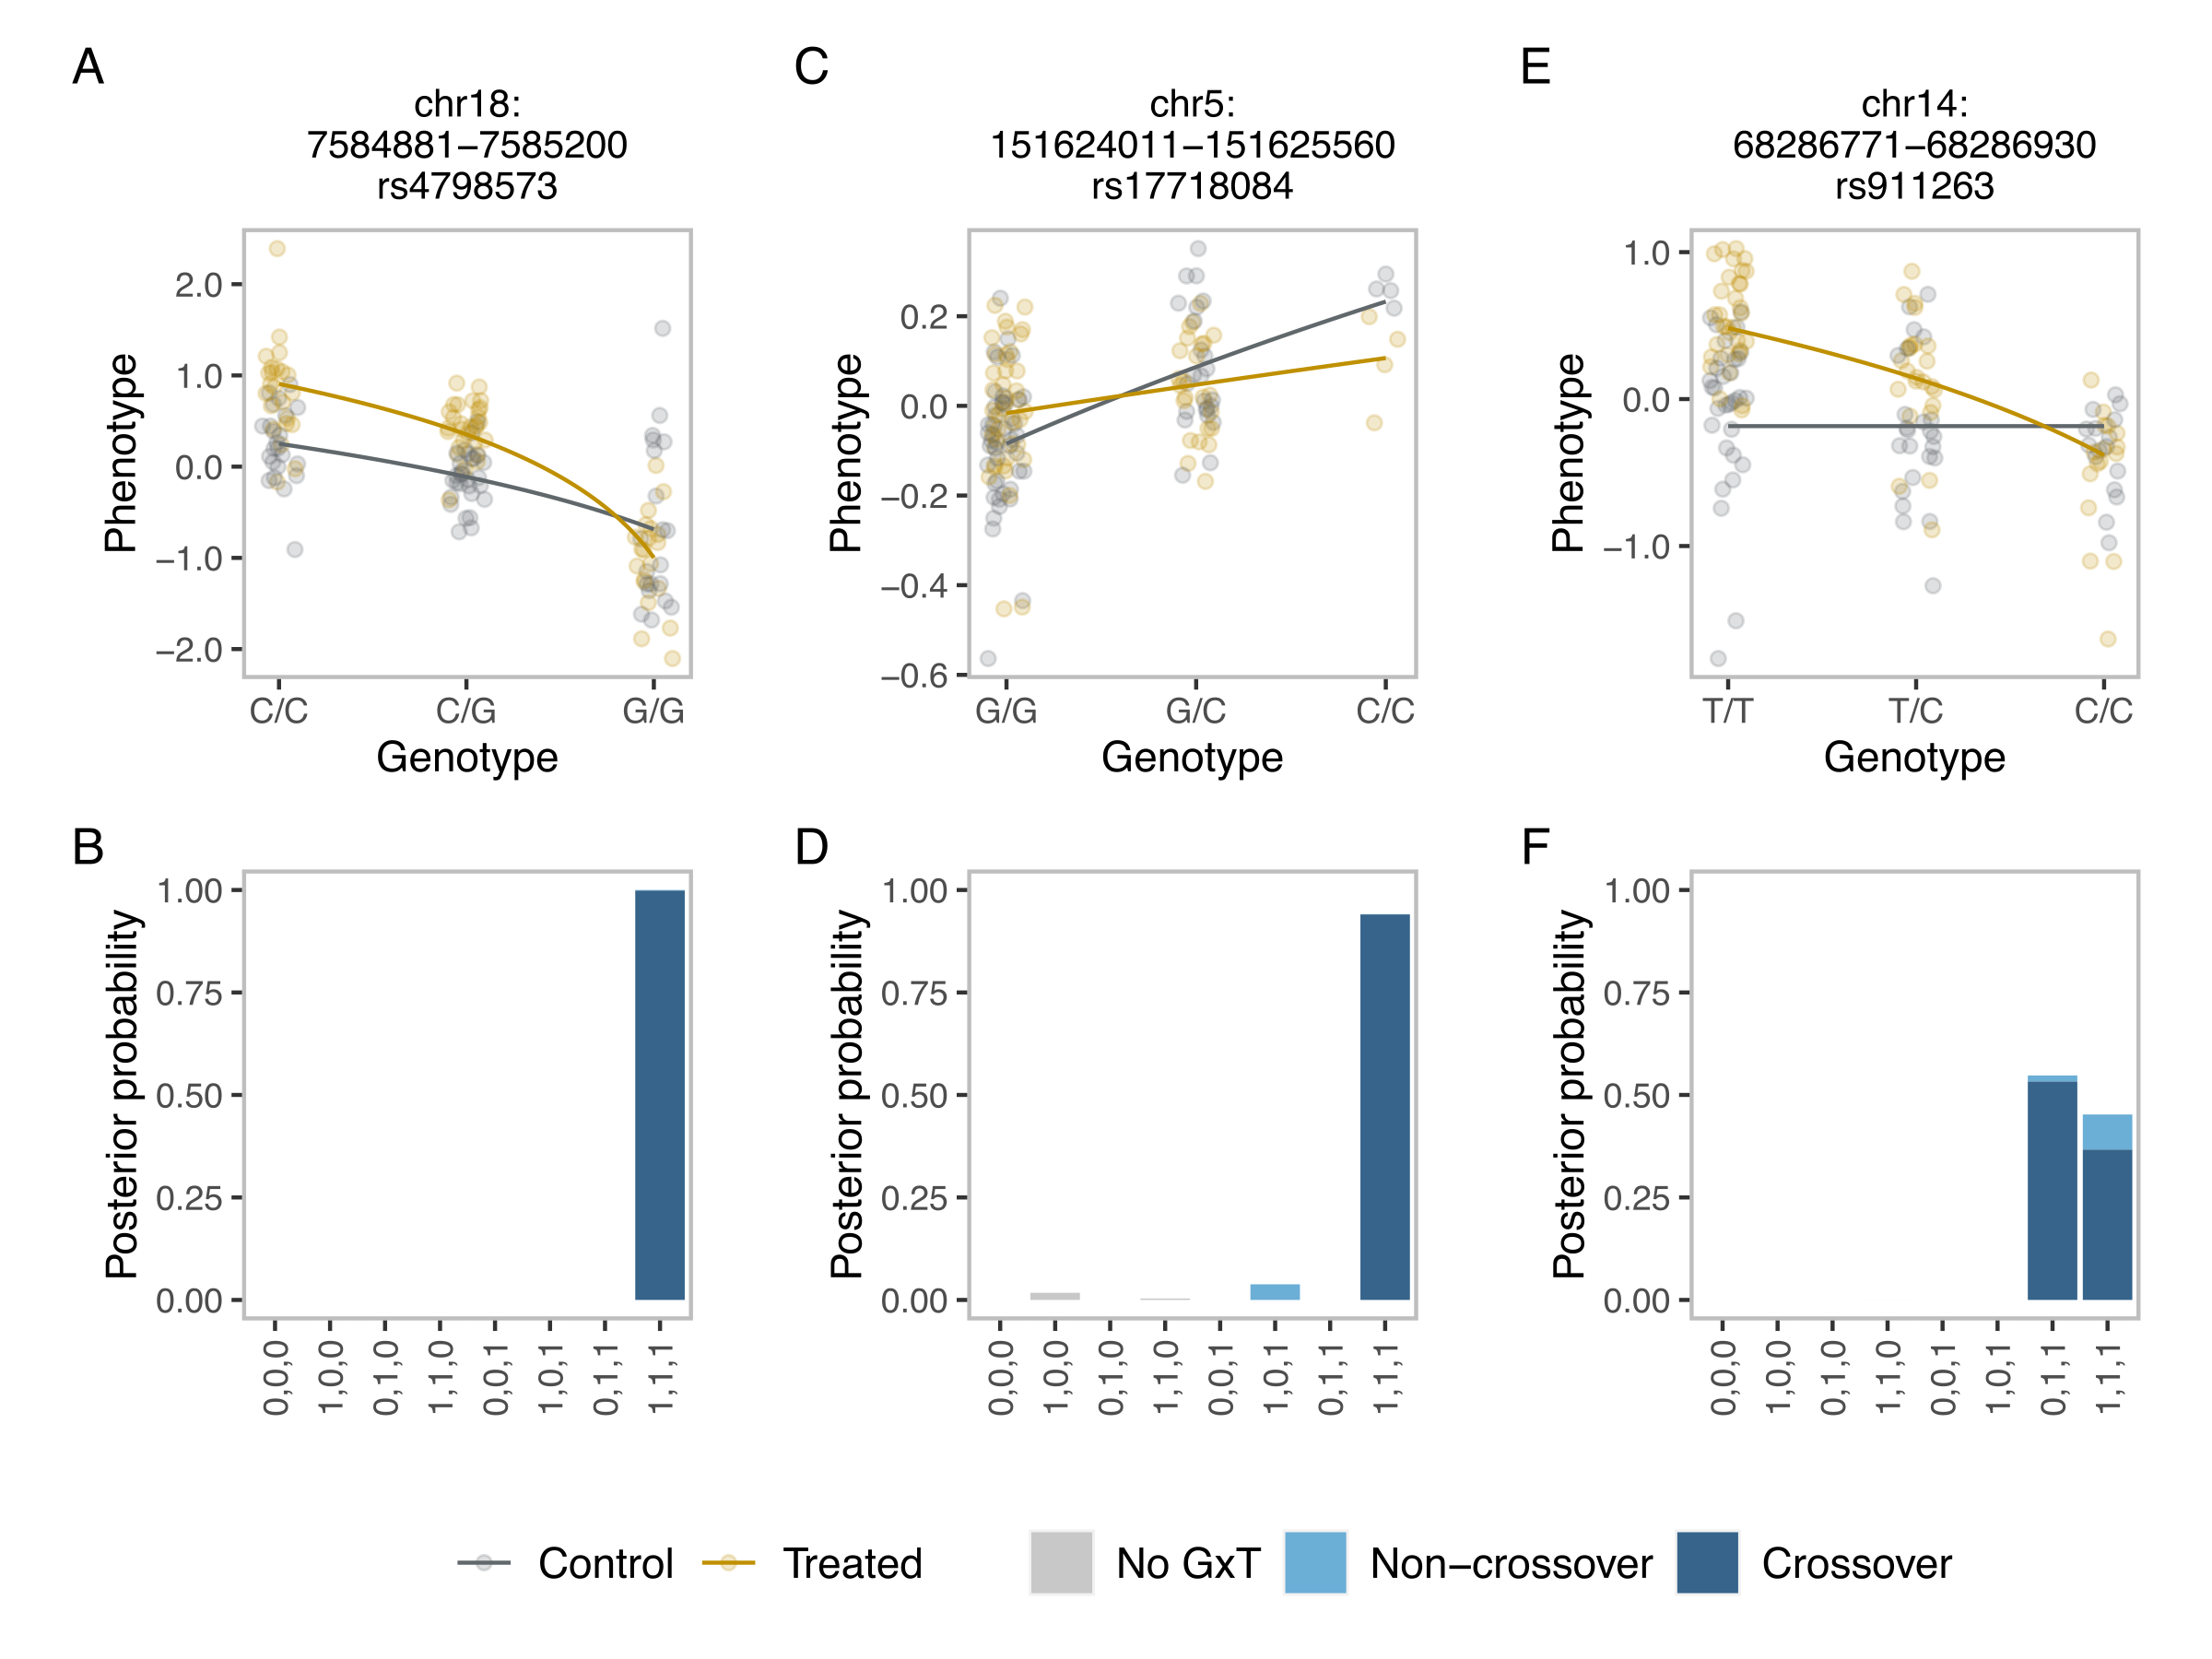
\includegraphics[width=0.9\textwidth]{png/wntatac_gp_co.png}
\end{center}  
\caption{
  {\bf
    S18 Fig.
    Examples of response caQTLs with the crossover interaction in hNPCs.}
The same as in \figwntrnadiv (see the main text) but for response caQTLs. 
}
\label{s-fig:wntatac-div}
\end{figure}

\end{document}
